% Select the PDF profile before \documentclass.
%
% The canonical build is PDF/UA-2 + PDF/A-4f with MathML structure
% elements and no formula /Alt entry.  The Ally profile targets the older
% PDF 1.7 / PDF/UA-1 model which Ally understands: hyperref can write the
% legacy DocInfo title and formulas carry /Alt entries instead of MathML.

\ifdefined\NTAllyCompatibilityBuild
\else
  \directlua{
    local profile = os.getenv("NT_PDF_PROFILE")
    if profile == "ally" then
      local slash = string.char(92)
      tex.sprint(slash .. "def" .. slash ..
        "NTAllyCompatibilityBuild{1}")
    elseif profile ~= nil and profile ~= "" and profile ~= "canonical" then
      tex.error("Unknown NT_PDF_PROFILE: " .. profile)
    end
  }
\fi

% Shared by both profiles and printed on the edition-information verso.
\def\NTPDFLanguage{en-US}

\ifdefined\NTAllyCompatibilityBuild
  % Machine-readable build facts reused by setup/versioning.tex.  Keep these
  % adjacent to the metadata they describe so the printed build information
  % cannot drift away from the PDF profile actually being selected.
  \def\NTPDFVersion{1.7}
  \def\NTPDFUAStandard{PDF/UA-1}
  \def\NTMathTaggingSetup{math/alt/use}
  \def\NTMathTaggingDescription{formula alternative text}

  \DocumentMetadata{
    lang          = \NTPDFLanguage,
    pdfversion    = 1.7,
    pdfstandard   = ua-1,
    tagging       = on,
    tagging-setup =
      { math/setup={},
        math/alt/use,
        extra-modules={verbatim-mo}}
  }
\else
  \def\NTPDFVersion{2.0}
  \def\NTPDFUAStandard{PDF/UA-2}
  \def\NTPDFAStandard{PDF/A-4f}
  \def\NTMathTaggingSetup{math/setup=mathml-SE}
  \def\NTMathTaggingDescription{MathML structure elements}

  \DocumentMetadata{
    lang          = \NTPDFLanguage,
    pdfversion    = 2.0,
    pdfstandard   = {ua-2,a-4f},
    tagging       = on,
    tagging-setup =
      { math/setup=mathml-SE,
        extra-modules={verbatim-mo}}
  }
\fi


\documentclass[
  10pt,
  letterpaper,
  twoside,
  openright
]{book}

\newcommand{\SeriesTitle}{The Great Story of Numbers}
  % Elementary Number Theory
  % Number Theory: A Narrative
  % Number Theory For All
  % The Great Story of Numbers

\newcommand{\VolumeTitle}{The Nature of Numbers}

\newcommand{\VolumeNumber}{1}

\newcommand{\DocumentTitle}{Book I of \SeriesTitle: \VolumeTitle}

\newcommand{\DocumentAuthor}{Egbert Rijke}

\title{\DocumentTitle}

\author{\DocumentAuthor}

\usepackage{fontspec}
\usepackage{mathtools}
\usepackage{lua-unicode-math}


\usepackage[dvipsnames]{xcolor}

\definecolor{CornflowerBlueHighContrast}{HTML}{007ACD}

\definecolor{grayblue}{HTML}{0047AB}

\definecolor{JHUBlue}{HTML}{002D72}

\definecolor{JHUSpiritBlue}{HTML}{68ACE5}


\directlua{
  fonts.handlers.otf.addfeature{
    name = "customkerns",
    type = "kern",
    data = {
      ["a"] = { ["b"] = -7, ["c"] = -10, ["d"] = -7, ["g"] = -3, ["p"] = -8, ["q"] = 5, ["s"] = -10, ["u"] = -30, ["v"] = -20, ["w"] = -17, ["y"] = -20},
      ["b"] = { ["a"] = -5, ["b"] = -12, ["e"] = -10, ["i"] = 15, ["l"] = -12, ["o"] = -23, ["r"] = -18, ["s"] = -14, ["u"] = -12, ["y"] = -18 },
      ["c"] = { ["a"] = 4, ["c"] = -5, ["e"] = -2, ["k"] = -11, ["o"] = -17, ["z"] = 15 },
      ["d"] = { ["e"] = -8, ["g"] = 10, ["o"] = -19, ["s"] = 15, ["y"] = 10 },
      ["e"] = { ["a"] = 10, ["c"] = -8, ["d"] = -12, ["e"] = 3, ["i"] = 10, ["o"] = 10, ["r"] = -6, ["s"] = -7 , ["v"] = 0, ["w"] = 0, ["x"] = 0, ["y"] = 20},
      ["f"] = { ["a"] = -10, ["e"] = 20, ["n"] = 40, ["o"] = 30, ["t"] = 50, ["u"] = 30, ["w"] = 80, ["y"] = 60 },
      ["g"] = { ["a"] = 0, ["e"] = 10, ["g"] = 30, ["i"] = 10, ["o"] = 15, ["r"] = 7, ["s"] = 15, ["u"] = 20, ["y"] = 50 },
      ["h"] = { ["a"] = -8, ["e"] = -10 },
      ["i"] = { ["c"] = 0, ["s"] = 10, ["x"] = 15 },
      ["k"] = { ["y"] = 0 },
      ["l"] = { ["o"] = -16, ["y"] = -12 },
      ["m"] = { ["e"] = -5, ["o"] = 10, ["s"] = 20 },
      ["n"] = { ["d"] = -13, ["e"] = -20, ["g"] = -26, ["k"] = -10, ["t"] = -20, ["y"] = -30 },
      ["o"] = { ["a"] = -23, ["b"] = -9, ["c"] = -14, ["d"] = 5, ["f"] = -17, ["g"] = 20, ["l"] = -14, ["n"] = -13, ["o"] = -12, ["r"] = -16, ["s"] = -8, ["t"] = 15, ["u"] = 0, ["w"] = -15, ["x"] = 20 },
      ["p"] = { ["a"] = -23, ["e"] = 0, ["h"] = -8, ["i"] = 10, ["o"] = 20, ["s"] = -17},
      ["q"] = { ["u"] = -5 },
      ["r"] = { ["a"] = -5, ["b"] = 10, ["c"] = -12, ["d"] = 20, ["e"] = 0, ["f"] = 20, ["i"] = 0, ["k"] = 15, ["n"] = 20, ["o"] = -26, ["r"] = 0, ["s"] = -11, ["u"] = 20, ["v"] = 20, ["y"] = 0 },
      ["s"] = { ["c"] = 0, ["e"] = 4, ["h"] = -12, ["i"] = -3, ["k"] = 10, ["n"] = 10, ["p"] = 20, ["s"] = -11, ["t"] = -2, ["u"] = -11, ["w"] = 20 },
      ["t"] = { ["b"] = 35, ["c"] = -5, ["e"] = -5, ["i"] = 20, ["o"] = -15, ["s"] = 20, ["u"] = 15, ["w"] = 30, ["y"] = 40, ["z"] = 15 },
      ["u"] = { ["b"] = -12, ["d"] = -13, ["e"] = -6, ["g"] = 10, ["l"] = -3, ["x"] = 10 },
      ["v"] = { ["a"] = 25, ["e"] = -2, ["i"] = 20, ["o"] = 20},
      ["w"] = { ["a"] = -23, ["e"] = -13, ["i"] = 20, ["o"] = -19},
      ["x"] = { ["a"] = 20, ["e"] = 15, ["i"] = 15,["t"] = 40, ["u"] = 10 },
      ["y"] = { ["a"] = -28, ["e"] = 20, ["i"] = 30, ["m"] = 10, ["n"] = 10, ["o"] = 10, ["p"] = 30, ["s"] = -23, ["t"] = 20 },
      ["z"] = { ["e"] = 15, ["i"] = 20, ["u"] = 10, ["y"] = 30, ["z"] = 10 },
      ["P"] = { ["a"] = -40, ["y"] = 30 },
      ["S"] = { ["e"] = 20 },
      ["T"] = { ["a"] = -30, ["w"] = 100, ["y"] = 100},
    }
  }
}


\directlua{
  fonts.handlers.otf.addfeature{
    name = "rijkeliga",
    type = "chainsubstitution",
    lookups = {
      {
        type = "ligature",
        data = {
          ["ij"] = { "i", "j" },
        }
      }
    },
    data = {
      rules = {
        {
          before  = { { "R" } },
          current = { { "i" }, { "j" } },
          after   = { { "k" }, { "e" } },
          lookups = { 1 }
        }
      }
    }
  }
}

\setmainfont{Libertinus Serif}[
  Numbers = OldStyle,
  Ligatures = {TeX, Common},
  ContextualAlternates = On,
  Kerning = On,
  StylisticSet = {6},
  RawFeature = {+customkerns,+rijkeliga},
  SmallCapsFeatures = {LetterSpace=2, Kerning=On},
]
\setmathfont{Libertinus Math}[Scale=MatchLowercase]
\setsansfont{Libertinus Sans}[Scale=MatchLowercase]
\setmonofont{Libertinus Mono}[Scale=MatchLowercase]

%\linespread{1.08}

\newcommand{\VersionFontName}{Libertinus}

\newfontfamily\mottofont{EB Garamond}[
  Numbers = OldStyle,
  Ligatures = {TeX, Common},
  ContextualAlternates = On,
  Kerning = On,
  Scale = 1.04,
  StylisticSet = {6},
  ItalicFeatures = {RawFeature={+customkerns}},
  SmallCapsFeatures = {LetterSpace=2, Kerning=On},
  ]
\newfontfamily\partdisplayfont{EB Garamond}[
  Numbers = OldStyle,
  Ligatures = {TeX, Common},
  ContextualAlternates = On,
  Kerning = On,
  Scale = 1.04,
  StylisticSet = {6},
  ItalicFeatures = {RawFeature={+customkerns}},
  SmallCapsFeatures = {LetterSpace=2, Kerning=On},
  ]
\newfontfamily\headerfont{EB Garamond}[
  Numbers = OldStyle,
  Ligatures = {TeX, Common},
  ContextualAlternates = On,
  Kerning = On,
  Scale = 1.04, StylisticSet = {6},
  SmallCapsFeatures = {LetterSpace=2, Kerning=On},
  ]

\newcommand{\otfrac}[2]{#1/#2}

\newcommand{\supst}{\textsuperscript{st}}

\newcommand{\supnd}{\textsuperscript{nd}}

\newcommand{\suprd}{\textsuperscript{rd}}

\newcommand{\supth}{\textsuperscript{th}}

\newfontfamily\greekfont{GFS Artemisia}[
  Scale=MatchLowercase,
  Script=Greek
]

\newcommand{\superhuge}{\fontsize{28}{34}\selectfont}

\newfontfamily{\coffeefont}{Libertinus Sans}

\ExplSyntaxOn

\clist_map_inline:nn
  {
    tiny,
    scriptsize,
    footnotesize,
    small,
    normalsize,
    large,
    Large,
    LARGE,
    huge,
    Huge
  }
  {
    \skip_new:c { #1baselineskip }
    \group_begin:
      \use:c { #1 }
      \skip_gset:cn { #1baselineskip } { \baselineskip }
    \group_end:
  }

\ExplSyntaxOff


\newfontfamily\cuneifont[
  Path = fonts/,
  Extension = .ttf,
  UprightFont = *-Regular
]{NotoSansCuneiform}

\ExplSyntaxOn

\tl_new:N \l__book_cuneiform_actualtext_tl

\NewDocumentCommand \cuneinumeral { m m }
  {
    \tl_set:Nx \l__book_cuneiform_actualtext_tl
      {
        cuneiform
        \c_space_tl
        numeral
        \c_space_tl
        #1
      }

    \tag_mc_end_push:

    \tag_mc_begin:n
      {
        tag        = Span,
        actualtext = \l__book_cuneiform_actualtext_tl
      }

    \group_begin:
      \cuneifont #2
    \group_end:

    \tag_mc_end:
    \tag_mc_begin_pop:n { }
  }

\ExplSyntaxOff


\usepackage[
  activate={true,nocompatibility},
  final,
  tracking=true,
  factor=1100,
  stretch=10,
  shrink=0
]{microtype}

\usepackage[ngerman,american]{babel}

\usepackage[autostyle=true,strict=true]{csquotes}
\MakeOuterQuote{"}

\usepackage[english]{selnolig}

\usepackage{realscripts}

\usepackage{impnattypo}

\usepackage[balanced]{lua-widow-control}
%\lwcsetup{draft}

\usepackage{fnpct}

%\usepackage[All]{lua-typo}

\UseMicrotypeSet[protrusion]{basicmath}

\frenchspacing
\emergencystretch=2em

\hyphenation{Py-tha-gorean}
\hyphenation{you-tube}

\addtolength{\abovedisplayskip}{2pt}
\addtolength{\belowdisplayskip}{2pt}
\addtolength{\abovedisplayshortskip}{2pt}
\addtolength{\belowdisplayshortskip}{2pt}




\usepackage{geometry}

\geometry{
  hcentering,
  letterpaper,
  textwidth=4.8in,
  includehead,
  headheight=14pt,
}

\AddToHook{cmd/chapter/after}{\thispagestyle{chapteropening}}

\usepackage{fancyhdr}

\fancyhf{}
\fancyhead[LE,RO]{\headerfont\thepage}
\fancyhead[RE]{\headerfont\scshape\lsstyle\nouppercase{\leftmark}}
\fancyhead[LO]{\headerfont\scshape\lsstyle\nouppercase{\rightmark}}
\renewcommand{\headrulewidth}{0pt}
\renewcommand{\footrulewidth}{0pt}
\pagestyle{fancy}

\fancypagestyle{plain}{%
  \fancyhf{}
  \fancyhead[LE,RO]{\headerfont\itshape\thepage}
  \fancyhead[RE]{\headerfont\itshape\nouppercase{\leftmark}}
  \fancyhead[LO]{\headerfont\itshape\nouppercase{\rightmark}}
  \renewcommand{\headrulewidth}{0pt}
  \renewcommand{\footrulewidth}{0pt}
}

\fancypagestyle{chapteropening}{
  \fancyhf{}
  \fancyfoot[C]{\thepage}
  \renewcommand{\headrulewidth}{0pt}
  \renewcommand{\footrulewidth}{0pt}
}

\makeatletter

\newcount\ConditionalBottomThreshold
\newbox\ConditionalBottomMeasure

\AddToHook{cmd/@make@normalcolbox/before}{%
  \ConditionalBottomThreshold=\vbadness
  \vbadness=10000
}

\AddToHook{cmd/@make@normalcolbox/after}{%
  \vbadness=\ConditionalBottomThreshold
  \ifnum\badness>\ConditionalBottomThreshold
    \ifnum\badness<10001
      \setbox\ConditionalBottomMeasure=\vbox{%
        \unvcopy\@outputbox
      }%
      \ifdim\ht\ConditionalBottomMeasure<\ht\@outputbox
        \setbox\@outputbox=\vbox to\ht\@outputbox{%
          \unvbox\@outputbox
          \vskip0pt plus .0001fil\relax
        }%
      \else
        \setbox\@outputbox=\vbox to\ht\@outputbox{%
          \unvbox\@outputbox
        }%
      \fi
    \fi
  \fi
}

\makeatother


\NewDocumentCommand{\HeadingRaggedRight}{}{%
  \raggedright
  \hyphenpenalty=10000
  \exhyphenpenalty=10000
  \relax
}

\EditInstance{heading}{chapter}{
  after-penalty-vspace = .1\textheight,
  after-vspace        = .2\textheight,
  heading-decls       = \normalfont\Large\HeadingRaggedRight,
  prefix-decls        = \scshape,
  number-decls        = \scshape,
  title-decls         = \normalfont\Huge\bfseries
}

\EditInstance{heading}{section}{
  heading-decls = \normalfont\Large\bfseries\HeadingRaggedRight
}

\EditInstance{heading}{subsection}{
  heading-decls = \normalfont\large\bfseries\HeadingRaggedRight
}

\NewDocumentCommand{\italicsection}{m}{%
  \section*[
    heading-decls={\normalfont\Large\mdseries\itshape\HeadingRaggedRight}
  ]{#1}%
}

\NewDocumentCommand{\italicsubsection}{m}{%
  \subsection*[
    heading-decls={\normalfont\large\mdseries\itshape\HeadingRaggedRight}
  ]{#1}%
}


\usepackage{enumext}

\renewcommand{\labelenumi}{\textup{(\roman{enumi})}}
\renewcommand{\labelenumii}{\textup{(\alph{enumii})}}
\renewcommand{\labelenumiii}{\textup{\arabic{enumiii}.}}

\renewcommand{\theenumi}{\roman{enumi}}
\renewcommand{\theenumii}{\alph{enumii}}
\renewcommand{\theenumiii}{\arabic{enumiii}}

\newenvironment{nobreakenumerate}
{
    \par
    \addvspace{\topsep}
    \noindent
    \begin{minipage}{\linewidth}
    \begin{enumerate}
}
{
    \end{enumerate}
    \end{minipage}
    \par
    \addvspace{\topsep}
}


\usepackage{array}
\usepackage{booktabs}


% Tagging-aware, book-local replacement for caption/subcaption.
% Target: LaTeX 2026-06-01 + latex-lab-float 0.81n + tagpdf 1.0e.
%
% Provides the subset used by The Great Story of Numbers:
%   subfigure environment
%   \subcaption[<short>]{<text>}
%   \phantomsubcaption
%   \subref and \subref*
%   \caption inside subfigure (locally = \subcaption)
%   \captionof{<type>} as a thin delegate to native \caption
%
% Ordinary \caption is NOT redefined globally.

\makeatletter
\ExplSyntaxOn

\AddToHook{cmd/@makecaption/before}[book/caption-font]
  {
    \str_if_eq:eeTF { \@captype } { subfigure }
      { \footnotesize }
      { \small }
  }

% --------------------------------------------------------------------------
% Counter/reference model formerly supplied by \DeclareCaptionSubType.
% --------------------------------------------------------------------------
\newcounter{subfigure}[figure]
\cs_set:Npn \thesubfigure { \alph{subfigure} }
\cs_set:Npn \p@subfigure { }
\cs_set:Npn \theHsubfigure { \theHfigure . \arabic{subfigure} }
\cs_set:Npn \subfigureautorefname { \figureautorefname }
\cs_set:Npn \fnum@subfigure { (\thesubfigure) }

% --------------------------------------------------------------------------
% Symbolic names used by latex-lab's native caption tagging sockets.
% A subfigure itself is deliberately a Part, as proposed by latex-lab-float;
% only its Caption and Lbl need symbolic names here.
% --------------------------------------------------------------------------
\NewStructureName{float/subfigure/caption}
\AssignStructureRole{float/subfigure/caption}{Caption}
\NewStructureName{float/subfigure/label}
\AssignStructureRole{float/subfigure/label}{Lbl}

% No separator after (a), matching
%   labelformat=parens, labelsep=none.
\NewSocketPlug{caption/label}{book-subfigure}
  { #1 }

% --------------------------------------------------------------------------
% State local to one subfigure environment.
% --------------------------------------------------------------------------
\tl_new:N   \l__book_subfigure_part_struct_tl
\tl_new:N   \l__book_subfigure_target_tl
\tl_new:N   \l__book_subfigure_outer_struct_tl
\tl_new:N   \l__book_subfigure_parent_ref_tl
\int_new:N  \l__book_subfigure_parent_counter_int
\bool_new:N \l__book_subfigure_caption_seen_bool
\bool_new:N \l__book_subfigure_active_bool
\bool_new:N \l__book_subfigure_bottom_fix_bool
\int_new:N  \g__book_subfigure_target_int

\msg_new:nnn { book-subfigure } { outside-float }
  {
    The~subfigure~environment~must~occur~inside~a~float~with~an~active~
    LaTeX~float~structure.
  }

\msg_new:nnn { book-subfigure } { subcaption-outside }
  { \string\subcaption~used~outside~a~subfigure~environment. }

% --------------------------------------------------------------------------
% zref-clever compatibility.
% This mirrors the compatibility information zref-clever normally installs
% when it detects the subcaption package.
% --------------------------------------------------------------------------
\cs_new_protected:Npn \__book_subfigure_setup_zref_clever:
  {
    \cs_if_exist:NT \zcsetup
      {
        \zcsetup
          {
            countertype   = { subfigure = figure },
            counterresetby = { subfigure = figure },
          }
      }
    \cs_if_exist:NT \zref@newprop
      {
        \zref@ifpropundefined{subref}
          { \zref@newprop{subref}{\thesubfigure} }
          { }
      }
  }
\AddToHook{begindocument/before}[book/subfigure-zref]
  { \__book_subfigure_setup_zref_clever: }

% --------------------------------------------------------------------------
% Label compatibility.
% The primary label keeps the full subfigure reference (e.g. 3.7a), while
% sub@<key> stores only a/b/... so existing \subref calls keep working.
% --------------------------------------------------------------------------
\cs_new_protected:Npn \__book_subfigure_saved_label: { }

\cs_new_protected:Npn \__book_subfigure_label:nn #1#2
  {
    % Write the ordinary label first, preserving its optional argument.
    \IfNoValueTF{#1}
      { \__book_subfigure_saved_label:{#2} }
      { \__book_subfigure_saved_label:[#1]{#2} }

    % Once a subcaption has stepped the counter, also create sub@<key>.
    \bool_if:NT \l__book_subfigure_caption_seen_bool
      {
        \group_begin:
          \protected@edef \@currentlabel { \thesubfigure }
          \__book_subfigure_saved_label:{sub@#2}
        \group_end:
      }
  }

\NewDocumentCommand \__book_subfigure_label { o m }
  { \__book_subfigure_label:nn {#1}{#2} }

% --------------------------------------------------------------------------
% Determine the reference prefix of the surrounding figure without stepping
% its counter.  In the usual source order (subfigures first, main caption
% afterwards), the parent number is the *next* figure number.  If the native
% main caption has already run, its latex-lab target tells us that the current
% figure number is already the right one.  This lets native \\caption remain
% completely untouched and step the outer figure exactly once.
% --------------------------------------------------------------------------
\cs_new_protected:Npn \__book_subfigure_set_parent_reference:
  {
    \tl_set:Ne \l__book_subfigure_outer_struct_tl
      { \@current@float@struct }
    \tl_if_eq:eeTF
      { \@currentHref }
      { figure.struct.\l__book_subfigure_outer_struct_tl }
      {
        \tl_set:Ne \l__book_subfigure_parent_ref_tl { \thefigure }
      }
      {
        \int_set:Nn \l__book_subfigure_parent_counter_int { \c@figure }
        \int_incr:N \c@figure
        \tl_set:Ne \l__book_subfigure_parent_ref_tl { \thefigure }
        \int_set:Nn \c@figure { \l__book_subfigure_parent_counter_int }
      }
    \cs_set:Npx \p@subfigure { \l__book_subfigure_parent_ref_tl }
  }

% --------------------------------------------------------------------------
% Counter step + hyperlink state shared by \subcaption and
% \phantomsubcaption.  We intentionally use the kernel refstepcounter, just
% as latex-lab's current native \caption does inside a float; the hyperlink
% target was already created at the beginning of this Part.
% --------------------------------------------------------------------------
\cs_new_protected:Npn \__book_subfigure_step:
  {
    \@kernel@refstepcounter{subfigure}

    \protected@edef\@currentlabel
      {
        \l__book_subfigure_parent_ref_tl
        \space
        (\thesubfigure)
      }

    \xdef\@currentHref{\l__book_subfigure_target_tl}
    \bool_set_true:N \l__book_subfigure_caption_seen_bool
  }

% --------------------------------------------------------------------------
% Label-only subcaption, optimized for the book's common \subcaption{} use.
% This avoids creating an empty P structure under Caption.
% --------------------------------------------------------------------------
\cs_new_protected:Npn \__book_subfigure_make_label_only_caption:
  {
    \footnotesize
    \vskip 6pt\relax
    \UseTaggingSocket{caption/begin}{\@current@float@struct}
    \global\@minipagefalse
    \hb@xt@\hsize
      {
        \hfil
        \UseTaggingSocket{caption/label/begin}
        \UseSocket{caption/label}{\fnum@subfigure}
        \UseTaggingSocket{caption/label/end}
        \hfil
      }
    \UseTaggingSocket{caption/end}
  }

% --------------------------------------------------------------------------
% \subcaption.  The optional short caption is accepted for source
% compatibility, but subcaptions are intentionally not written to the LoF,
% matching subcaption's default list=false.
% --------------------------------------------------------------------------
\cs_new_protected:Npn \__book_subfigure_caption:nn #1#2
  {
    \bool_if:NTF \l__book_subfigure_active_bool
      {
        \__book_subfigure_step:
        \cs_set:Npn \@currentlabelname {#2}
        \AssignSocketPlug{caption/label}{book-subfigure}
        \setlength\abovecaptionskip{6pt}
        \setlength\belowcaptionskip{0pt}
        \tl_if_blank:nTF {#2}
          { \__book_subfigure_make_label_only_caption: }
          { \@makecaption{\fnum@subfigure}{#2} }
      }
      { \msg_error:nn { book-subfigure } { subcaption-outside } }
  }

\NewDocumentCommand \subcaption { o m }
  { \__book_subfigure_caption:nn {#1}{#2} }

\NewDocumentCommand \phantomsubcaption { }
  {
    \bool_if:NTF \l__book_subfigure_active_bool
      { \__book_subfigure_step: }
      { \msg_error:nn { book-subfigure } { subcaption-outside } }
  }

% --------------------------------------------------------------------------
% \subref compatibility.  Default output is a/b/...; the unstarred form
% hyperlinks the whole reference to the beginning of the subfigure Part.
% An optional argument is accepted for compatibility with subcaption syntax.
% --------------------------------------------------------------------------
\NewDocumentCommand \subref { s o m }
  {
    \IfBooleanTF{#1}
      {
        \zcref*
          [
            noname,
            ref = subref,
            refbounds = {,(,),}
          ]
          {#3}
      }
      {
        \zcref
          [
            noname,
            ref = subref,
            refbounds = {,(,),}
          ]
          {#3}
      }
  }

% --------------------------------------------------------------------------
% Minipage setup.  Supports the usual subcaption/minipage forms
%   \begin{subfigure}[t]{.48\textwidth}
%   \begin{subfigure}[t][<height>]{<width>}
%   \begin{subfigure}[t][<height>][c]{<width>}
% including subcaption's T/B alignment conveniences.
% --------------------------------------------------------------------------
\cs_new_protected:Npn \__book_subfigure_begin_minipage:nnnn #1#2#3#4
  {
    \bool_set_false:N \l__book_subfigure_bottom_fix_bool
    \str_case:nnF {#1}
      {
        {T}
          {
            \IfNoValueTF{#2}
              { \begin{minipage}[t]{#4} }
              {
                \IfNoValueTF{#3}
                  { \begin{minipage}[t][#2]{#4} }
                  { \begin{minipage}[t][#2][#3]{#4} }
              }
            \vspace{0pt}
          }
        {B}
          {
            \IfNoValueTF{#2}
              { \begin{minipage}[b]{#4} }
              {
                \IfNoValueTF{#3}
                  { \begin{minipage}[b][#2]{#4} }
                  { \begin{minipage}[b][#2][#3]{#4} }
              }
            \bool_set_true:N \l__book_subfigure_bottom_fix_bool
          }
      }
      {
        \IfNoValueTF{#2}
          { \begin{minipage}[#1]{#4} }
          {
            \IfNoValueTF{#3}
              { \begin{minipage}[#1][#2]{#4} }
              { \begin{minipage}[#1][#2][#3]{#4} }
          }
      }
  }

\cs_new_protected:Npn \__book_subfigure_begin:nnnn #1#2#3#4
  {
    \tl_if_exist:NTF \@current@float@struct
      {
        \tl_if_empty:NTF \@current@float@struct
          { \msg_error:nn { book-subfigure } { outside-float } }
          {
            \bool_set_true:N  \l__book_subfigure_active_bool
            \bool_set_false:N \l__book_subfigure_caption_seen_bool
            \__book_subfigure_set_parent_reference:

            % One Part per subfigure, exactly as proposed by latex-lab-float.
            \tag_struct_begin:n { tag=Part }
            \tl_set:Ne \l__book_subfigure_part_struct_tl
              { \tag_get:n { struct_num } }

            % Use a dedicated target counter, mirroring latex-lab-float's own
            % link-target strategy.  Creating it while Part is current lets
            % tagpdf associate the destination with this structure.
            \int_gincr:N \g__book_subfigure_target_int
            \tl_set:Ne \l__book_subfigure_target_tl
              { subfigure.structure.\int_use:N\g__book_subfigure_target_int }
            \MakeLinkTarget*{\l__book_subfigure_target_tl}

            \__book_subfigure_begin_minipage:nnnn {#1}{#2}{#3}{#4}

            % The minipage is now the layout box; semantically its captions
            % belong to the surrounding Part, not to the outer Figure.
            \cs_set:Npn \@captype { subfigure }
            \tl_set:NV \@current@float@struct
              \l__book_subfigure_part_struct_tl

            % Preserve the source-level subcaption API locally.
            \cs_set_eq:NN \caption \subcaption
            \cs_set_eq:NN \__book_subfigure_saved_label: \label
            \cs_set_eq:NN \label \__book_subfigure_label

            % Mirror zref-clever's subcaption compatibility hook.
            \cs_if_exist:NT \zref@localaddprop
              { \zref@localaddprop \ZREF@mainlist { subref } }
          }
      }
      { \msg_error:nn { book-subfigure } { outside-float } }
  }

\cs_new_protected:Npn \__book_subfigure_end:
  {
    \bool_if:NT \l__book_subfigure_active_bool
      {
        \bool_if:NT \l__book_subfigure_bottom_fix_bool { \vspace{0pt} }
        \end{minipage}
        \tag_struct_end:
      }
  }

\NewDocumentEnvironment{subfigure}{ O{b} o o m }
  { \__book_subfigure_begin:nnnn {#1}{#2}{#3}{#4} }
  { \__book_subfigure_end: }

% --------------------------------------------------------------------------
% Minimal replacement for caption's \captionof, because the book uses it in
% minipages inside a figure.  It does not implement captions: it merely sets
% \@captype and delegates immediately to native \caption.  The surrounding
% minipage supplies the intended local scope, and a following \label sees the
% native caption's reference state.
% --------------------------------------------------------------------------
\ProvideDocumentCommand \captionof { m }
  {
    \cs_set:Npn \@captype {#1}
    \caption
  }

\ExplSyntaxOff
\makeatother


\usepackage{float}

\setcounter{topnumber}{1}
\setcounter{bottomnumber}{1}
\setcounter{totalnumber}{1}

\usepackage{graphicx}
\graphicspath{{figures/}}

\usepackage{tikz}
\usetikzlibrary{
  angles,
  arrows.meta,
  babel,
  backgrounds,
  calc,
  decorations.markings,
  decorations.pathreplacing,
  decorations.pathmorphing,
  hobby,
  intersections,
  quotes,
  shapes.geometric,
  trees}
\usepackage{pgfplots}
\pgfplotsset{compat=1.18}
\tikzset{every picture/.append style={line cap=round, line join=round}}

\makeatletter
\newcommand{\TikZFontSizes}{%
  \renewcommand\normalsize{\@setfontsize\normalsize{9pt}{10.8pt}}%
  \renewcommand\small{\@setfontsize\small{8.1pt}{9.9pt}}%
  \renewcommand\footnotesize{\@setfontsize\footnotesize{7.2pt}{8.55pt}}%
  \renewcommand\scriptsize{\@setfontsize\scriptsize{6.3pt}{7.2pt}}%
  \renewcommand\tiny{\@setfontsize\tiny{4.5pt}{5.4pt}}%
  \renewcommand\large{\@setfontsize\large{10.8pt}{12.6pt}}%
  \renewcommand\Large{\@setfontsize\Large{12.96pt}{16.2pt}}%
  \renewcommand\LARGE{\@setfontsize\LARGE{15.552pt}{19.8pt}}%
  \renewcommand\huge{\@setfontsize\huge{18.666pt}{22.5pt}}%
  \renewcommand\Huge{\@setfontsize\Huge{22.392pt}{27pt}}%
  \normalsize
}
\makeatother

\tikzset{
  every picture/.append style={
    execute at begin picture=\TikZFontSizes
  }
}

\pgfplotsset{
  lectureplot/.style={
    width=12cm, height=8cm,
    axis lines=middle,
    axis line style={-stealth},
    tick style={draw=none},
    xlabel={$x$}, ylabel={$y$},
    xmin=0, xmax=1e6,
    ymin=0, ymax=8.5e4,
    clip=false,
    legend style={
      draw=none,                               
      fill=none,
      font=\footnotesize,
      at={(0.05,0.95)},                        
      anchor=north west,
      /tikz/every even column/.append style={column sep=1em}
    },
    legend cell align=left
  }
}

\newcommand{\arrowpairsep}{4pt}
\newcommand{\arrowpairshortentip}{4mm}
\newcommand{\arrowpairshortenbutt}{5mm}
\newcommand{\arrowpairmaskwidth}{3pt}

\newcommand{\arrowpairover}[2]{%
  \path let
    \p1=(#1.center),
    \p2=(#2.center),
    \n1={atan2(\y2-\y1,\x2-\x1)}
  in
  \pgfextra{%
    \foreach \shift/\direction/\shortenstart/\shortenend in {
      90/{|->}/4mm/4mm,
      -90/{<-|}/4mm/4.5mm
    } {%
      \begin{scope}[
        transform canvas={
          shift={({\n1+\shift}:\arrowpairsep)}
        }
      ]
        \draw[
          white,
          line width=\arrowpairmaskwidth,
          bend left=10,
          shorten <=\shortenstart,
          shorten >=\shortenend
        ]
          (#1.center) to (#2.center);
        \draw[
          \direction,
          thick,
          bend left=10,
          shorten <=\shortenstart,
          shorten >=\shortenend
        ]
          (#1.center) to (#2.center);
      \end{scope}
    }%
  };
}


\setlength{\jot}{5pt}

\newlength{\casesleftsep}
\newlength{\casescolsep}

\setlength{\casesleftsep}{0.2em} % distance from brace to first column
\setlength{\casescolsep}{1.2em}   % distance between the two columns

\renewenvironment{cases}
  {\left\{\,
   \begin{array}{
     @{\hspace{\casesleftsep}} l
     @{\hspace{\casescolsep}} l
     @{}
   }}
  {\end{array}\right.}


\usepackage{amsmath}
\usepackage{amsthm}

\newtheorem{theorem}{Theorem}[section]
\newtheorem{lemma}[theorem]{Lemma}
\newtheorem{proposition}[theorem]{Proposition}
\newtheorem{corollary}[theorem]{Corollary}
\newtheorem{conjecture}{Conjecture}
\newtheorem{problem}[conjecture]{Problem}

\theoremstyle{definition}
\newtheorem{definition}[theorem]{Definition}
\newtheorem{example}[theorem]{Example}

\theoremstyle{remark}
\newtheorem{remark}[theorem]{Remark}


\usepackage{totcount}

\newtotcounter{exercisecounter}
\AtEndDocument{%
  \typeout{Total number of exercises: \number\value{exercisecounter}}%
}

\newcounter{currentchaptex}

\newcommand{\exercises}{%
  \par\clearpage%
  \phantomsection%
  \section*{Exercises}%
  \addcontentsline{toc}{section}{Exercises}%
  \markboth{\leftmark}{\MakeUppercase{Exercises}}%
  \setcounter{currentchaptex}{0}
}

\newcommand{\exercise}{\stepcounter{exercisecounter}\item}

\newenvironment{exenum}
{\begin{enumext}[
    label=\thechapter.\arabic*,
    ref=\thechapter.\arabic*,
    widest=99,
    labelsep=.6em,
    noitemsep]}
{\end{enumext}}

\newenvironment{subexenum}
{\begin{enumext}[
    label=(\alph*),
    ref=\thechapter.\arabic{enumXi}(\alph*),
    noitemsep]}
{\end{enumext}}

\newenvironment{starter}
{%
  \italicsubsection{Starter Exercises}%
  \begin{exenum}
  \setcounter{enumXi}{\value{currentchaptex}}
}
{%
  \setcounter{currentchaptex}{\value{enumXi}}
  \end{exenum}
}

\newenvironment{foundational}
{%
  \italicsubsection{Foundational Exercises}%
  \begin{exenum}
  \setcounter{enumXi}{\value{currentchaptex}}
}
{%
  \setcounter{currentchaptex}{\value{enumXi}}
  \end{exenum}
}

\newenvironment{routine}
{%
  \italicsubsection{Routine-Building Exercises}%
  \begin{exenum}
  \setcounter{enumXi}{\value{currentchaptex}}
}
{%
  \setcounter{currentchaptex}{\value{enumXi}}
  \end{exenum}
}

\newenvironment{challenge}
{%
  \italicsubsection{Challenge Exercises}%
  \begin{exenum}
  \setcounter{enumXi}{\value{currentchaptex}}
}
{%
  \setcounter{currentchaptex}{\value{enumXi}}
  \end{exenum}
}


\usepackage[backend=biber, style=alphabetic, sorting=nyt]{biblatex}

\addbibresource{src/references.bib}

\setcounter{biburlnumpenalty}{7000}
\setcounter{biburllcpenalty}{7000}
\setcounter{biburlucpenalty}{7000}

\appto{\bibsetup}{\emergencystretch=3em}

\DeclareLabelalphaTemplate{%
  \labelelement{%
    \field[final]{shorthand}%
    \field{label}%
    \field[strwidth=3,strside=left,ifnames=1]{labelname}%
    \field[strwidth=1,strside=left]{labelname}%
  }%
  \labelelement{%
    \field{year}%
  }%
}

\DeclareFieldFormat{labelalpha}{\textsc{\lsstyle #1}}

\renewcommand{\mkbibnamefamily}[1]{\textsc{#1}}

\renewcommand{\mkbibnameprefix}[1]{\textsc{#1}}

\DeclareFieldFormat{journaltitle}{#1}

\DeclareFieldFormat{issuetitle}{#1}

\DeclareFieldFormat{edition}{#1\isdot~\bibstring{edition}}

% \DeclareFieldFormat{isbn}{\textsf{\textsc{isbn}}\addcolon\space #1}

% \DeclareFieldFormat{issn}{\textsf{\textsc{issn}}\addcolon\space #1}

% \DeclareFieldFormat{doi}{%
%   \textsf{\textsc{doi}}\addcolon\space
%   \ifhyperref
%     {\href{https://doi.org/#1}{\nolinkurl{#1}}}
%     {\nolinkurl{#1}}}

% \DeclareFieldFormat{url}{%
%   \textsf{\textsc{url}}\addcolon\space
%   \ifhyperref
%     {\href{#1}{\nolinkurl{#1}}}
%     {\nolinkurl{#1}}}

\DeclareFieldFormat{eprint:arxiv}{%
  \textsc{arXiv}\addcolon\space
  \ifhyperref{\href{https://arxiv.org/abs/#1}{\nolinkurl{#1}}}{\nolinkurl{#1}}%
  \iffieldundef{eprintclass}{}{\addspace\mkbibbrackets{\thefield{eprintclass}}}}

\DeclareFieldFormat
  [article,inbook,incollection,inproceedings,misc,unpublished]
  {title}{\mkbibemph{#1}}

\setlength{\bibitemsep}{0.5\baselineskip}
\setlength{\bibhang}{1.5em}


\usepackage{xurl}

% \usepackage{hyperref}
% \hypersetup{
%   hidelinks,
%   pdftitle          = {The Great Story of Numbers},
%   pdfauthor         = {Egbert Rijke},
%   pdfsubject        = {Number Theory Course Notes},
%   pdfdisplaydoctitle = true,
% }

\usepackage[pdfusetitle]{hyperref}

\hypersetup{
  pdfdisplaydoctitle = true,
  colorlinks=true,
  linktoc=all,
  allcolors=CornflowerBlue,
  pdfsubject  = {Course Notes},
  pdfkeywords = {number theory, introduction to number theory, introduction to proof,history of number theory, Euclid, Fibonacci, Fermat, Euler, Gauss, mathematical induction, Euclidean algorithm, modular arithmetic, Pythagorean triples, infinite descent, prime numbers, multiplicative functions, strong divisibility sequences, Fermat's little theorem, Fermat's two-squares theorem, polynomials, cyclotomic polynomials, Zsigmondy's theorem, Vantieghem's theorem, quadratic residues, quadratic reciprocity, quadratic fields},
}

\usepackage{zref-titleref}
\usepackage{zref-clever}
\usepackage{zref-xr}

\zcsetup{
  cap,
  noabbrev,
  nameinlink,
}

\zxrsetup{
  toltxlabel = true
}

\makeatletter
\ExplSyntaxOn

\AddToHook{cmd/ParseLaTeXeTheoremlike/after}
  {
    \tl_if_novalue:oTF \l__block_note_tl
      { }
      {
        \exp_args:NV
          \zref@titleref@setcurrent
          \l__block_note_tl
      }
  }

\ExplSyntaxOff
\makeatother

\newcommand{\zcrefnamed}[1]{\zcref{#1}\space(\ztitleref{#1})}

\zcRefTypeSetup{enumXi}{Name-sg = Exercise, Name-pl = Exercises}
\zcRefTypeSetup{enumXii}{Name-sg = Exercise, Name-pl = Exercises}


\ExplSyntaxOn
\NewDocumentCommand{\DeclareSemanticSymbol}{mm}
{
  \tag_if_active:TF
  {
    \tag_mc_begin:n { tag=Span, actualtext = #2 }
    #1
    \tag_mc_end:
  }
  {
    #1
  }
}
\ExplSyntaxOff

\ExplSyntaxOn

\NewDocumentCommand \dotsofwidth { m }
  {
    \hbox_set:Nn \l_tmpa_box { $#1$ }
    \mathrel
      {
        \hbox_to_wd:nn { \box_wd:N \l_tmpa_box }
          { \hfil $\vdots$ \hfil }
      }
  }

\ExplSyntaxOff

\newcommand{\rpermutation}[2]{{}_{#1}P_{#2}}

\renewcommand{\pmod}[1]{\mkern5mu\left(\operatorname{mod} \mkern 6mu #1\right)}

\DeclareMathOperator{\ord}{ord}

\DeclareMathOperator{\ind}{ind}

\DeclareMathOperator*{\lcm}{lcm}

\DeclareMathOperator{\sgn}{sgn}

\DeclareMathOperator{\rad}{rad}

\DeclarePairedDelimiter{\legendredelim}{(}{)}

\newcommand{\legendre}[2]{%
  \DeclareSemanticSymbol{%
    \legendredelim*{\genfrac{}{}{}{}{#1}{#2}}%
  }{the Legendre symbol of #1 over #2}%
}

\newcommand{\abssep}{\mkern2mu}
\DeclarePairedDelimiterX{\abs}[1]{\lvert}{\rvert}{\abssep #1\abssep}

\newcommand{\lres}[2]{%
  \DeclareSemanticSymbol{%
    \lfloor #1 \rceil_{#2}%
  }{the least absolute residue of #1 modulo #2}%
}

\newcommand{\abslres}[2]{%
  \DeclareSemanticSymbol{%
    \ensuremath{|\mkern-3mu \lfloor #1 \rceil\mkern-3mu |_{#2}}
}{the absolute value of the least absolute residue of #1 modulo #2}}

\newcommand{\complementsubset}[1]{%
  \DeclareSemanticSymbol{#1^{\mathrm{c}}}{the complement of #1}}

\newcommand{\Oh}{\DeclareSemanticSymbol{\mathord{O}}{big Oh}}

\newcommand{\oh}{\DeclareSemanticSymbol{\mathord{o}}{little Oh}}

\newcommand{\blank}{\DeclareSemanticSymbol{\mathord{\hspace{1pt}\text{--}\hspace{1pt}}}{blank}}

\newcommand{\apart}{\DeclareSemanticSymbol{\mathbin{\#}}{is apart from}}

\DeclareMathOperator{\numerator}{num}

\DeclareMathOperator{\denominator}{denom}

\setmathfont[range=\triangledown]{STIX Two Math}

\newcommand{\mediant}{\DeclareSemanticSymbol{\mathbin{\triangledown}}{mediant}}

\newcommand{\bimapsto}{%
  \DeclareSemanticSymbol{%
    \mathrel{\vcenter{\offinterlineskip\ialign{##\cr$\mapsfrom$\cr\noalign{\kern0pt}$\mapsto$\cr}}}
  }{maps to and comes from}
}

\newcommand{\content}{\DeclareSemanticSymbol{\mathrm{cont}}{the content of}}

\newcommand{\floorfrac}[2]{\DeclareSemanticSymbol{\left\lfloor\frac{#1}{#2}\right\rfloor}{the largest integer less than or equal to}}

\newcommand{\totient}{\DeclareSemanticSymbol{\phi}{totient}}

\newcommand{\im}{\mathrm{im}}


\newif\ifshownotes

% \shownotestrue
\shownotesfalse

\usepackage{environ}
\NewEnviron{noteblock}{%
  \ifshownotes
    \begingroup\color{black!60}\BODY\endgroup
  \fi
}

\newcommand{\note}[1]{%
  \ifshownotes
    \begingroup\color{black!60}#1\endgroup
  \fi
}


\newcommand{\TwoDigits}[1]{\ifnum#1<10 0\fi\number#1}

\newcommand{\TodayYYMMDD}{%
  \TwoDigits{\numexpr\year-2000\relax}%
  \TwoDigits{\month}%
  \TwoDigits{\day}%
}

\newcommand{\Version}[1]{Version #1.\TodayYYMMDD~~~~\VersionFontName}


\newcommand{\Sierpinski}{Sierpiński}


\ExplSyntaxOn

\NewDocumentCommand \ShowTagParaBalance { m }
  {
    \iow_term:x
      {
        TAGPARA~#1:~
        outer~
        \int_use:N \g__tag_para_begin_int /
        \int_use:N \g__tag_para_end_int;~
        inner~
        \int_use:N \g__tag_para_main_begin_int /
        \int_use:N \g__tag_para_main_end_int
      }
  }

\ExplSyntaxOff


% Install after the rest of the preamble: % Install after the rest of the preamble: \input{setup/typographic-metrics}
% Keep typographic-metrics.lua in the same setup/ directory.
% The module observes nodes; it changes neither typesetting nor PDF tagging.
\ifdefined\directlua\else
  \PackageError{typographic-metrics}{LuaLaTeX is required}{}
\fi

\directlua{NTTypometrics = require("setup.typographic-metrics")}

\AddToHook{cmd/mainmatter/before}[nt-metrics-start]
  {\par\begingroup\normalfont\normalsize\directlua{NTTypometrics.start()}\endgroup}
\AddToHook{cmd/backmatter/before}[nt-metrics-stop]
  {\par\directlua{NTTypometrics.stop()}}

% Sectioning marks the next paragraph(s) as potential heading material.
% Lua detects the return to body text; no private book-class command is used.
\AddToHook{cmd/part/before}[nt-metrics-part-head-in]
  {\par\directlua{NTTypometrics.heading_begin()}}
\AddToHook{cmd/chapter/before}[nt-metrics-chapter-head-in]
  {\par\directlua{NTTypometrics.heading_begin()}}
\AddToHook{cmd/section/before}[nt-metrics-section-head-in]
  {\par\directlua{NTTypometrics.heading_begin()}}
\AddToHook{cmd/subsection/before}[nt-metrics-subsection-head-in]
  {\par\directlua{NTTypometrics.heading_begin()}}
\AddToHook{cmd/subsubsection/before}[nt-metrics-subsubsection-head-in]
  {\par\directlua{NTTypometrics.heading_begin()}}

% Captions inside floats and other floating material are not book prose.
\AddToHook{env/figure/begin}[nt-metrics-figure-in]
  {\directlua{NTTypometrics.exclude_begin()}}
\AddToHook{env/figure/end}[nt-metrics-figure-out]
  {\directlua{NTTypometrics.exclude_end()}}
\AddToHook{env/figure*/begin}[nt-metrics-figure-star-in]
  {\directlua{NTTypometrics.exclude_begin()}}
\AddToHook{env/figure*/end}[nt-metrics-figure-star-out]
  {\directlua{NTTypometrics.exclude_end()}}
\AddToHook{env/table/begin}[nt-metrics-table-in]
  {\directlua{NTTypometrics.exclude_begin()}}
\AddToHook{env/table/end}[nt-metrics-table-out]
  {\directlua{NTTypometrics.exclude_end()}}
\AddToHook{env/table*/begin}[nt-metrics-table-star-in]
  {\directlua{NTTypometrics.exclude_begin()}}
\AddToHook{env/table*/end}[nt-metrics-table-star-out]
  {\directlua{NTTypometrics.exclude_end()}}
\AddToHook{env/longtable/begin}[nt-metrics-longtable-in]
  {\directlua{NTTypometrics.exclude_begin()}}
\AddToHook{env/longtable/end}[nt-metrics-longtable-out]
  {\directlua{NTTypometrics.exclude_end()}}

% For a caption outside a float (or another passage to omit), wrap it in this.
\NewDocumentEnvironment{NTMetricsExclude}{}
  {\directlua{NTTypometrics.exclude_begin()}}
  {\directlua{NTTypometrics.exclude_end()}}

% Run after the final shipout, so page-density figures include the last page.
\AddToHook{enddocument/afterlastpage}[nt-metrics-report]
  {\directlua{NTTypometrics.report()}}

% Keep typographic-metrics.lua in the same setup/ directory.
% The module observes nodes; it changes neither typesetting nor PDF tagging.
\ifdefined\directlua\else
  \PackageError{typographic-metrics}{LuaLaTeX is required}{}
\fi

\directlua{NTTypometrics = require("setup.typographic-metrics")}

\AddToHook{cmd/mainmatter/before}[nt-metrics-start]
  {\par\begingroup\normalfont\normalsize\directlua{NTTypometrics.start()}\endgroup}
\AddToHook{cmd/backmatter/before}[nt-metrics-stop]
  {\par\directlua{NTTypometrics.stop()}}

% Sectioning marks the next paragraph(s) as potential heading material.
% Lua detects the return to body text; no private book-class command is used.
\AddToHook{cmd/part/before}[nt-metrics-part-head-in]
  {\par\directlua{NTTypometrics.heading_begin()}}
\AddToHook{cmd/chapter/before}[nt-metrics-chapter-head-in]
  {\par\directlua{NTTypometrics.heading_begin()}}
\AddToHook{cmd/section/before}[nt-metrics-section-head-in]
  {\par\directlua{NTTypometrics.heading_begin()}}
\AddToHook{cmd/subsection/before}[nt-metrics-subsection-head-in]
  {\par\directlua{NTTypometrics.heading_begin()}}
\AddToHook{cmd/subsubsection/before}[nt-metrics-subsubsection-head-in]
  {\par\directlua{NTTypometrics.heading_begin()}}

% Captions inside floats and other floating material are not book prose.
\AddToHook{env/figure/begin}[nt-metrics-figure-in]
  {\directlua{NTTypometrics.exclude_begin()}}
\AddToHook{env/figure/end}[nt-metrics-figure-out]
  {\directlua{NTTypometrics.exclude_end()}}
\AddToHook{env/figure*/begin}[nt-metrics-figure-star-in]
  {\directlua{NTTypometrics.exclude_begin()}}
\AddToHook{env/figure*/end}[nt-metrics-figure-star-out]
  {\directlua{NTTypometrics.exclude_end()}}
\AddToHook{env/table/begin}[nt-metrics-table-in]
  {\directlua{NTTypometrics.exclude_begin()}}
\AddToHook{env/table/end}[nt-metrics-table-out]
  {\directlua{NTTypometrics.exclude_end()}}
\AddToHook{env/table*/begin}[nt-metrics-table-star-in]
  {\directlua{NTTypometrics.exclude_begin()}}
\AddToHook{env/table*/end}[nt-metrics-table-star-out]
  {\directlua{NTTypometrics.exclude_end()}}
\AddToHook{env/longtable/begin}[nt-metrics-longtable-in]
  {\directlua{NTTypometrics.exclude_begin()}}
\AddToHook{env/longtable/end}[nt-metrics-longtable-out]
  {\directlua{NTTypometrics.exclude_end()}}

% For a caption outside a float (or another passage to omit), wrap it in this.
\NewDocumentEnvironment{NTMetricsExclude}{}
  {\directlua{NTTypometrics.exclude_begin()}}
  {\directlua{NTTypometrics.exclude_end()}}

% Run after the final shipout, so page-density figures include the last page.
\AddToHook{enddocument/afterlastpage}[nt-metrics-report]
  {\directlua{NTTypometrics.report()}}


% fractions.tex
% Fraction geometry for LuaLaTeX + unicode-math.
%
% Load this file after the final \setmathfont declaration.  In the
% number-theory source tree, setup/mathematics.tex is already loaded after
% setup/fonts.tex, so it is a suitable place to \input this file.
%
% The code changes only LuaTeX's native OpenType-math geometry parameters.
% It does not redefine \frac, \dfrac, \tfrac, \genfrac, \binom, etc., and
% therefore leaves LaTeX/LuaMML's semantic math structure untouched.

\ExplSyntaxOn

\msg_new:nnn { number-theory } { fractions-luatex-only }
  {
    The~number-theory~fraction~geometry~layer~requires~LuaLaTeX.
  }

\msg_new:nnn { number-theory } { fractions-unicode-math-required }
  {
    The~number-theory~fraction~geometry~layer~requires~unicode-math~and~must~be~
    loaded~after~the~math~font~has~been~selected.
  }

\msg_new:nnn { number-theory } { fractions-local-inside-math }
  {
    A~local~fraction-geometry~scope~must~enclose~the~complete~math~formula,~
    not~start~inside~an~already-open~formula.~LuaTeX~consults~these~math~
    parameters~when~the~whole~math~list~is~converted.~Use~the~local~scope~
    around~$...$,~\(...\),~\[...\],~or~the~display~environment.
  }

\sys_if_engine_luatex:F
  { \msg_fatal:nn { number-theory } { fractions-luatex-only } }

\cs_if_exist:NF \Umathfractiondenomdown
  { \msg_fatal:nn { number-theory } { fractions-unicode-math-required } }
\cs_if_exist:NF \crampedtextstyle
  { \msg_fatal:nn { number-theory } { fractions-unicode-math-required } }

\bool_new:N \l__nt_fraction_global_bool

% LuaTeX's \Umath... parameter scanner expects a real math-style command.
% Therefore these scratch control sequences are aliases, not macros expanding
% to style commands.
\cs_new_eq:NN \l__nt_fraction_style:         \displaystyle
\cs_new_eq:NN \l__nt_fraction_cramped_style: \crampeddisplaystyle

\cs_new_protected:Npn \__nt_fraction_select_style:NN #1#2
  {
    \cs_set_eq:NN \l__nt_fraction_style:         #1
    \cs_set_eq:NN \l__nt_fraction_cramped_style: #2
  }

\cs_new_protected:Npn \__nt_fraction_assign_one:NNn #1#2#3
  {
    \bool_if:NT \l__nt_fraction_global_bool { \tex_global:D }
    #1 #2 = \dim_eval:n {#3} \scan_stop:
  }

\cs_new_protected:Npn \__nt_fraction_set:Nn #1#2
  {
    \__nt_fraction_assign_one:NNn
      #1 \l__nt_fraction_style: {#2}
    \__nt_fraction_assign_one:NNn
      #1 \l__nt_fraction_cramped_style: {#2}
  }

\cs_new_protected:Npn \__nt_fraction_adjust_one:NNn #1#2#3
  {
    \dim_set:Nn \l_tmpa_dim
      { \tex_the:D #1 #2 + ( #3 ) }
    \__nt_fraction_assign_one:NNn #1 #2 { \l_tmpa_dim }
  }

\cs_new_protected:Npn \__nt_fraction_adjust:Nn #1#2
  {
    \__nt_fraction_adjust_one:NNn
      #1 \l__nt_fraction_style: {#2}
    \__nt_fraction_adjust_one:NNn
      #1 \l__nt_fraction_cramped_style: {#2}
  }

% Keys for one math style.
%
% Ordinary ruled fractions use the fraction parameters.  A generalized
% fraction with zero rule thickness (notably \binom) uses the stack parameters.
% delimiter-size controls the minimum delimiter size used by generalized
% fractions with delimiters.
\keys_define:nn { number-theory / fractions / style }
  {
    numerator-shift .code:n =
      { \__nt_fraction_set:Nn \Umathfractionnumup {#1} },
    numerator-shift-adjust .code:n =
      { \__nt_fraction_adjust:Nn \Umathfractionnumup {#1} },

    denominator-shift .code:n =
      { \__nt_fraction_set:Nn \Umathfractiondenomdown {#1} },
    denominator-shift-adjust .code:n =
      { \__nt_fraction_adjust:Nn \Umathfractiondenomdown {#1} },

    numerator-gap .code:n =
      { \__nt_fraction_set:Nn \Umathfractionnumvgap {#1} },
    numerator-gap-adjust .code:n =
      { \__nt_fraction_adjust:Nn \Umathfractionnumvgap {#1} },

    denominator-gap .code:n =
      { \__nt_fraction_set:Nn \Umathfractiondenomvgap {#1} },
    denominator-gap-adjust .code:n =
      { \__nt_fraction_adjust:Nn \Umathfractiondenomvgap {#1} },

    rule-thickness .code:n =
      { \__nt_fraction_set:Nn \Umathfractionrule {#1} },
    rule-thickness-adjust .code:n =
      { \__nt_fraction_adjust:Nn \Umathfractionrule {#1} },

    stack-numerator-shift .code:n =
      { \__nt_fraction_set:Nn \Umathstacknumup {#1} },
    stack-numerator-shift-adjust .code:n =
      { \__nt_fraction_adjust:Nn \Umathstacknumup {#1} },

    stack-denominator-shift .code:n =
      { \__nt_fraction_set:Nn \Umathstackdenomdown {#1} },
    stack-denominator-shift-adjust .code:n =
      { \__nt_fraction_adjust:Nn \Umathstackdenomdown {#1} },

    stack-gap .code:n =
      { \__nt_fraction_set:Nn \Umathstackvgap {#1} },
    stack-gap-adjust .code:n =
      { \__nt_fraction_adjust:Nn \Umathstackvgap {#1} },

    delimiter-size .code:n =
      { \__nt_fraction_set:Nn \Umathfractiondelsize {#1} },
    delimiter-size-adjust .code:n =
      { \__nt_fraction_adjust:Nn \Umathfractiondelsize {#1} },
  }

\cs_new_protected:Npn \__nt_fraction_style_keys:NNn #1#2#3
  {
    \__nt_fraction_select_style:NN #1#2
    \keys_set:nn { number-theory / fractions / style } {#3}
  }

\keys_define:nn { number-theory / fractions }
  {
    display .code:n =
      {
        \__nt_fraction_style_keys:NNn
          \displaystyle \crampeddisplaystyle {#1}
      },
    text .code:n =
      {
        \__nt_fraction_style_keys:NNn
          \textstyle \crampedtextstyle {#1}
      },
    inline .code:n =
      {
        \__nt_fraction_style_keys:NNn
          \textstyle \crampedtextstyle {#1}
      },
    script .code:n =
      {
        \__nt_fraction_style_keys:NNn
          \scriptstyle \crampedscriptstyle {#1}
      },
    scriptscript .code:n =
      {
        \__nt_fraction_style_keys:NNn
          \scriptscriptstyle \crampedscriptscriptstyle {#1}
      },
  }

% Permanent document-wide setup.
\NewDocumentCommand \NTFractionSetup { m }
  {
    \group_begin:
      \bool_set_true:N \l__nt_fraction_global_bool
      \keys_set:nn { number-theory / fractions } {#1}
    \group_end:
  }

% Local setup.  The scope must begin outside math mode so that the parameter
% values are still in force when LuaTeX converts the completed math list.
\NewDocumentCommand \NTWithFractionSetup { m m }
  {
    \mode_if_math:T
      { \msg_warning:nn { number-theory } { fractions-local-inside-math } }
    \group_begin:
      \bool_set_false:N \l__nt_fraction_global_bool
      \keys_set:nn { number-theory / fractions } {#1}
      #2
    \group_end:
  }

\NewDocumentEnvironment { ntfractionsetup } { m }
  {
    \mode_if_math:T
      { \msg_warning:nn { number-theory } { fractions-local-inside-math } }
    \group_begin:
      \bool_set_false:N \l__nt_fraction_global_bool
      \keys_set:nn { number-theory / fractions } {#1}
  }
  { \group_end: }

% Diagnostic output: report the current native parameters in the .log file.
\cs_new_protected:Npn \__nt_fraction_show_one:NNn #1#2#3
  {
    \iow_term:x
      { NT~FRACTIONS~|~#3~=~\tex_the:D #1 #2 }
  }

\cs_new_protected:Npn \__nt_fraction_show_style:NNn #1#2#3
  {
    \__nt_fraction_show_one:NNn \Umathfractionnumup       #1 { #3/numerator-shift }
    \__nt_fraction_show_one:NNn \Umathfractiondenomdown   #1 { #3/denominator-shift }
    \__nt_fraction_show_one:NNn \Umathfractionnumvgap     #1 { #3/numerator-gap }
    \__nt_fraction_show_one:NNn \Umathfractiondenomvgap   #1 { #3/denominator-gap }
    \__nt_fraction_show_one:NNn \Umathfractionrule        #1 { #3/rule-thickness }
    \__nt_fraction_show_one:NNn \Umathstacknumup          #1 { #3/stack-numerator-shift }
    \__nt_fraction_show_one:NNn \Umathstackdenomdown      #1 { #3/stack-denominator-shift }
    \__nt_fraction_show_one:NNn \Umathstackvgap           #1 { #3/stack-gap }
    \__nt_fraction_show_one:NNn \Umathfractiondelsize     #1 { #3/delimiter-size }
    \__nt_fraction_show_one:NNn \Umathfractionnumup       #2 { #3-cramped/numerator-shift }
    \__nt_fraction_show_one:NNn \Umathfractiondenomdown   #2 { #3-cramped/denominator-shift }
  }

\NewDocumentCommand \NTFractionShow { }
  {
    \__nt_fraction_show_style:NNn
      \displaystyle \crampeddisplaystyle { display }
    \__nt_fraction_show_style:NNn
      \textstyle \crampedtextstyle { text }
    \__nt_fraction_show_style:NNn
      \scriptstyle \crampedscriptstyle { script }
    \__nt_fraction_show_style:NNn
      \scriptscriptstyle \crampedscriptscriptstyle { scriptscript }
  }

\ExplSyntaxOff

\NTFractionSetup{
  text = {
    denominator-shift-adjust = -2pt,
  },
}




\makeatletter

\zref@newprop{volchapter}[0]{\number\value{chapter}}
\zref@newprop{volnextpage}[1]{\number\value{page}}

\NewDocumentCommand{\SaveVolumeChapterState}{m}{%
  \cleardoublepage
  \zref@wrapper@immediate{%
    \zref@labelbyprops
      {volume-chapter:#1}
      {volchapter}%
  }%
}

\NewDocumentCommand{\SaveVolumePageState}{m}{%
  \cleardoublepage
  \zref@wrapper@immediate{%
    \zref@labelbyprops
      {volume-page:#1}
      {volnextpage}%
  }%
}

\NewDocumentCommand{\ContinueFromVolume}{m}{%
  \zref@ifrefundefined{volume-chapter:#1}{%
    \PackageError{number-theory}
      {Missing chapter state for #1}
      {Build the preceding volume first.}%
  }{}%
  \zref@ifrefundefined{volume-page:#1}{%
    \PackageError{number-theory}
      {Missing page state for #1}
      {Build the preceding volume first.}%
  }{}%
  \setcounter{chapter}{%
    \zref@extractdefault
      {volume-chapter:#1}
      {volchapter}
      {0}%
  }%
  \setcounter{page}{%
    \zref@extractdefault
      {volume-page:#1}
      {volnextpage}
      {1}%
  }%
}

\makeatother


\ExternalVolume{2}

\ExternalVolume{3}

\begin{document}

\pagestyle{empty}
\hypersetup{pageanchor=false}

\begin{titlepage}
  \begin{center}
    {\Huge\textsc{Johns Hopkins University}\par}
    \vspace*{\stretch{1}}
    {\Huge\textbf{\DocumentAuthor}\par}
    \vspace*{\stretch{1}}
    \begin{center}
      \begin{tikzpicture}[
        alt={
          A circle of radius square root of 10 is displayed on a Cartesian grid.
          On the circle, a sequence of open dots are displayed with arrows
          from each dot to the next, until the last dot is reached, which is a
          solid dot.
          The arrows from one dot to the next are obtained by tracing out the
          unique line between it and the nearest lattice point, and it is
          targeting the second intersection on the circle.
          The solid dot is itself a lattice point, so this process terminates
          there.
        }
        ]
        
        \draw[gray,very thin] (-4.1,-4.1) grid[step=1] (4.1,4.1);
        
        \draw[thick] (0,0) circle ({sqrt(10)});
        
        \draw[->] (-4.2,0) -- (4.2,0);
        \draw[->] (0,-4.2) -- (0,4.2);
        
        \coordinate (P5) at (-3,-1);
        \draw[fill=black,thick] (P5) circle (2pt);
        
        \coordinate (R5) at ({-1401/3305},{-10357/3305});
        \coordinate (R4) at ({1401/653},{-1517/653});
        \coordinate (R3) at ({-13/41},{129/41});
        \coordinate (R2) at ({13/5},{9/5});
        \coordinate (R1) at ({-3},{-1});
        \coordinate (Q5) at ({0},{-3});
        \coordinate (Q4) at ({2},{-2});
        \coordinate (Q3) at (0,3);
        \coordinate (Q2) at (3,2);
        \draw[DarkOrchid,very thick,->,shorten >=1.5ex] (R5) -- (R4);
        \draw[Green,very thick,->,shorten >=1ex] (R4) -- (R3);    
        \draw[YellowOrange,very thick,->,shorten >=1.5ex] (R3) -- (R2);
        \draw[CornflowerBlue,very thick,->,shorten >=1ex] (Q2) -- (R1);
        \draw[fill=white,thick] (R5) circle (2pt);
        \draw[fill=white,thick] (R4) circle (2pt);
        \draw[fill=white,thick] (R3) circle (2pt);
        \draw[fill=white,thick] (R2) circle (2pt);
        \draw[fill=DarkOrchid,draw=DarkOrchid,thick] (Q5) circle (2pt);
        \draw[fill=Green,draw=Green,thick] (Q4) circle (2pt);
        \draw[fill=YellowOrange,draw=YellowOrange,thick] (Q3) circle (2pt);
        \draw[fill=CornflowerBlue,draw=CornflowerBlue,thick] (Q2) circle (2pt);
        \draw[fill=white,thick] (R2) circle (2pt);
      \end{tikzpicture}
    \end{center}
    \vspace*{\stretch{.5}}
    {\superhuge \textbf{\VolumeTitle}\par}
    \vspace*{\stretch{1}}
    {\Large \textsc{Book I}\par}
    \vspace*{\stretch{.5}}
    {\Large \textsc{of}\par}
    \vspace*{\stretch{1}}
    {\huge \textsc{\SeriesTitle}}
  \end{center}
\end{titlepage}


\thispagestyle{empty}
\null
\vfill

\begingroup
\setlength{\parindent}{0pt}
Version: \VersionIdentifier\par
Primary font: \VersionFontName\par
Supporting fonts:
\NTRecordedSupportingFontFamilies\par
TeX engine: \NTTeXEngineInformation\par
LaTeX format: \NTLaTeXFormatInformation\par
Document language: \NTPDFLanguage\par
PDF version: \NTPDFVersion\par
Accessibility standard: \NTPDFUAStandard\par
\ifdefined\NTPDFAStandard
  Archival standard: \NTPDFAStandard\par
  \fi
Tagging setup: \NTMathTaggingDescription\space
  (\NTMathTaggingSetup)\par
\endgroup

\vspace{\baselineskip}

\begingroup
\setlength{\parindent}{0pt}
Citing this work:\par
\medskip
\begingroup
\small
\ttfamily
\raggedright
\parskip=0pt
\parindent=0pt
@book\{rijke-\VersionIdentifier,\par
  \hangindent=2em\hangafter=1\hspace*{1em}%
    author       = \{\DocumentAuthor\},\par
  \hangindent=2em\hangafter=1\hspace*{1em}%
    title        = \{\DocumentTitle\},\par
  \hangindent=2em\hangafter=1\hspace*{1em}%
    year         = \{\number\year\},\par
  \hangindent=2em\hangafter=1\hspace*{1em}%
    month        = \ifcase\month\or jan\or feb\or mar\or apr\or may\or jun\or
      jul\or aug\or sep\or oct\or nov\or dec\fi,\par
  \hangindent=2em\hangafter=1\hspace*{1em}%
    note         = \{Version \VersionIdentifier\},\par
  \hangindent=2em\hangafter=1\hspace*{1em}%
    url          = \{https://egbertrijke.github.io/notes/number-theory/\}\par    
  \}\par
\endgroup
\endgroup


\cleardoublepage

\frontmatter

\hypersetup{pageanchor=true}

\pagestyle{fancy}

\tableofcontents
\listoffigures

\chapter{Introduction}\label{chapter:introduction}
\markboth{%
  \MakeUppercase{\itshape Introduction}%
}{}

Number theory is the study of numbers, particularly the natural numbers
\begin{equation*}
  0,1,2,\ldots
\end{equation*}
increasing indefinitely in increments of $1$, the integers 
\begin{equation*}
  \ldots, -2, -1, 0, 1, 2, \ldots,
\end{equation*}
and occasionally the rational numbers (fractions of integers). Its central themes include questions about divisibility, modular arithmetic, prime numbers, arithmetic functions, and finding integer solutions to equations. Additionally, number theory explores the question whether numbers can be represented in a certain form, such as a sum of two, three, or four squares, as a product or sum of primes, or as the area of a Pythagorean triangle. Paired with such representability questions is the combinatorial question of determining the number of ways a number can be so represented. More advanced branches of number theory are occasionally also concerned with obtaining quantitative bounds or other forms of approximation of certain aspects of numbers, which naturally leads to the use of other number systems, such as the real numbers, complex numbers, or $p$-adic numbers. However, in \emph{elementary number theory} these explorations are primarily motivated by how these number systems relate back to the integers.

The diversity of the kinds of questions described above has led to a wealth of mathematical techniques, methods of proof, and advanced concepts, and number theory remains a very active field of study to this day. The aim of this course is to introduce some of the most fundamental ideas upon which number theory is built. Some of these ideas you might already know or have heard about: prime numbers are the building blocks of numbers; mathematical induction is a proof technique to formally prove properties of all natural numbers; and the idea that some of the most frequently occurring numbers can be arranged geometrically such as in triangles, squares, pentagons, and so on. An important aspect of the course is to learn how to make these intuitive ideas mathematically precise. Once we have developed a solid foundation, we will start building the edifice of number theory.

Concretely, we set out the following learning objectives for this course:
\begin{itemize}
\item Explain the structure of different number systems such as the natural numbers, the integers, the rational numbers, modular arithmetic, and the Gaussian integers, along with the methods of proof for properties involving each of them.
\item Write mathematically rigorous proofs which demonstrate a clear progression of ideas and clearly state the principles of proof involved such as unique existence, mathematical induction, the well-ordering theorem, and the method of infinite descent.
\item Solve some challenging number-theoretic problems, including selected contest-style problems.
\item Apply some of the central theorems of elementary number theory, including Fermat's little theorem, Fermat's two-squares theorem, quadratic reciprocity, and Pell's equation.
%\item Situate core results of number theory in their historical context, and clarify the progression of ideas that led to the modern perspective.
\end{itemize}


% \section*{Overview of the Course}

% An integer $a$ is said to \emph{divide} an integer $b$ if there exists an integer $x$ such that $ax=b$. In other words, the number $a$ divides $b$ if the equation
% \begin{equation*}
%   ax=b  
% \end{equation*}
% has a solution in the integers. In this case we say that $a$ is a \emph{divisor} of $b$, and we write $a \mid b$. This equation is the simplest example of a Diophantine equation. Diophantine equations are equations expressed using variables, integers, and arithmetic operations. The primary goal of solving a Diophantine equation is to find integers for each of the variables for which the equation is true. The study of Diophantine equations is a cornerstone of number theory.

% For example, the equation
% \begin{equation*}
%   x^2 - 1 = 0
% \end{equation*}
% is a \emph{quadratic Diophantine equation} with two solutions: $x=\pm 1$. One of the most well-known quadratic Diophantine equations is the equation
% \begin{equation*}
%   x^2 + y^2 = z^2,
% \end{equation*}
% which is a Diophantine equation in \emph{three variables}. Its solutions are known as \emph{Pythagorean triples}. These triples, such as $(3,4,5)$ and $(5,12,13)$, corresponds to the side lengths of right-angled triangles and have been studied since antiquity. Perhaps the most famous Diophantine equation is Fermat's equation
% \begin{equation*}
%   x^n + y^n = z^n,
% \end{equation*}
% which has no solutions for nonzero integers $x$, $y$, and $z$ when $n\geq 3$.

% In this course, however, we will not go as far as proving Fermat's last theorem. The first target of this course is the Fundamental Theorem of Arithmetic, which establishes the prime numbers as the building blocks of all natural numbers. A number $n$ is said to be prime if it has exactly one divisor $d \mid n$ such that $d\neq n$. If this is the case, then its unique divisor that is not equal to itself is the number $1$. The Fundamental Theorem of Arithmetic asserts that any nonzero natural number $n$ can be written as a product of primes
% \begin{equation*}
%   n=p_1p_2\cdots p_k,
% \end{equation*}
% and that this decomposition of $n$ as a product of primes is unique up to the ordering of the primes.

% In order to study divisibility properties more deeply, Gauss introduced in his \textsc{Disquisitiones Arithmeticae} the congruence relations of modular arithmetic. Following Gauss, we say that a number $a$ is congruent to $b$ modulo $n$, that is,
% \begin{equation*}
%   a \equiv b \pmod{n}
% \end{equation*}
% if $n \mid b - a$. Gauss used this new formalism to study quadratic residues, the Chinese Remainder theorem, and a variety of other problems in number theory, a thread we will also pick up on in this course.

% Some of the most important theorems in this context are Fermat's Little Theorem, Euler's Theorem, and Wilson's Theorem. Fermat's theorem asserts that given any prime number $p$ and any number $a$ that is not divisible by $p$ we have
% \begin{equation*}
%   a^{p-1}\equiv 1 \pmod{p}.
% \end{equation*}
% Fermat's theorem is an important ingredient in primality tests: If the congruence $a^{n-1}\equiv 1 \pmod{n}$ is false then the number $n$ cannot be prime. Testing this congruence for several values of $a$ is a simple way of discovering that $n$ is composite. This test is by itself, however, not conclusive because there are some numbers, the Carmichael numbers, that satisfy Fermat's congruence for all $a$ relatively prime to $n$.

% Euler's theorem is a sharper version of Fermat's Little Theorem, but it involves a new function: \emph{Euler's totient function}. Euler's totient function $\phi$ counts the numbers less than $n$ that are relatively prime to $n$, which means that they share no common divisors with $n$ other than $1$. For example, if $p$ is a prime number then $\phi(p)=p-1$ since every number $0<n<p$ is relatively prime to $p$. Using the totient function, Euler's theorem asserts that the congruence relation
% \begin{equation*}
%   a^{\phi(n)}\equiv 1 \pmod{n}
% \end{equation*}
% holds for any natural number $n$ and any number $a$ relatively prime to $n$. Euler's theorem has applications in cryptography.

% Wilson's Theorem states that a number $p$ is a prime number if and only if the congruence
% \begin{equation*}
%   (p-1)!\equiv -1 \pmod{p}
% \end{equation*}
% holds. Here, the exclamation mark is used for the \emph{factorial function}: The number $n!$ is the product $1\cdots n$ of all the numbers from $1$ through $n$. Wilson's Theorem therefore gives another criterion for primality testing.

% Euler's totient function is an example of an arithmetic function. Other such functions include the function $\tau(n)$, which returns the number of divisors of a number $n$, the function $\sigma(n)$, which returns the sum of the divisors of a number $n$, and the \emph{M\"obius function} $\mu$. These and other functions have important relations between them, that we will investigate next. The M\"obius inversion formula, for instance, states that if $f$ and $g$ are two arithmetic functions, then we have
% \begin{equation*}
%   f(n)=\sum_{d\mid n} g(d)\qquad\text{if and only if}\qquad g(n)=\sum_{d\mid n}\mu(d)f\left(\frac{n}{d}\right).
% \end{equation*}
% This result allows us to "invert" summation relations involving divisors.

% The M\"obius inversion is only one aspect of an algebraic structure that is present on the set of all arithmetic functions. Arithmetic functions can be multiplied by an operation known as \emph{Dirichlet convolution}, which gives the set of arithmetic functions the structure of a \emph{commutative ring}. Commutative rings are sets with operations of addition and multiplication satisfying the usual laws of arithmetic, and having such a structure on a set gives us a great opportunity to study them further. In our case, we get to study the primes more closely.

% Experimentation is essential in number theory. By making lists of primes, lists of numbers that can be written as the sum of two squares or sums of three squares, lists of square-free numbers, and so on, you will start to gather data on numbers and perhaps start seeing patterns that might otherwise feel elusive. At the end of this section, we have produced two number grids with the numbers from $1$ to $1584$. The great masters all have endlessly created such lists to organize and discover patterns in various kinds of numbers. Feel free to print it as many times as you like, and color them according to your own rules, or whenever something in the course piques your interest. Some exercises throughout the course will ask you to color this number grid in a certain way.

\section*{Literature}

This course was originally designed to follow \cite{andrews1994} fairly closely. One distinctive feature of this book is that it presents many of the most important theorems from two perspectives: a combinatorial one and an abstract one. This dual approach helps to clarify not only why these results are true but also appreciate why they are natural and inevitable within the broader framework of mathematics.

From the Fall semester of 2025 onwards, the course was redesigned to follow \cite{silverman2012}. Silverman's book encourages the reader to explore numbers, hypothesize their properties and relations, and effectively teaches students how to generate ideas towards proving number-theoretic theorems. It is written a very accessible, conversational style, with practical examples and exercises.

There are many further excellent sources to learn number theory from. One of my personal favorites for its clarity and accessibility is LeVeque's \textsc{Topics in Number Theory} \cite{leveque1956vol1,leveque1956vol2}. Both Andrews', Silverman's, and LeVeque's textbooks contain plenty of exercises, most of which are very fun.

The undisputed classic textbook on number theory, which is warmly recommended for any aspiring number theorist, is Hardy and Wright's \textsc{Introduction to the Theory of Numbers} \cite{hardy2008}. This book covers all the essential topics in number theory, including elementary number theory and analytical number theory. It is more comprehensive and also provides more historical notes. The textbook of Hardy and Wright does not provide exercises, but it contains the proofs of many important facts in number theory that are stated as exercises elsewhere.

% \section*{Online resources}

% There are plenty of ways to learn number theory and engage with communities of mathematicians and students online. First and foremost, \emph{Wikipedia} has many excellent pages on topics from and related to number theory. The website \emph{math.stackexchange.com} is dedicated to answering any kind of mathematical question, although more research-oriented questions are usually posed on \emph{mathoverflow.net}. The website \emph{artofproblemsolving.com} is dedicated to contest mathematics and the problem-solving techniques necessary to do well in competitions such as the International Mathematical Olympiad.

% Furthermore, there are some popular channels on video-sharing sites such as YouTube, Twitch, and TikTok. We mention some of the most notable:

% \begin{enumerate}
% \item Lectures:
% \begin{enumerate}
% \item \emph{Richard Borcherds} is a Fields Medalist who has recorded many of his Berkeley lectures and made them available on YouTube. The topics of his lectures are always well-motivated and presented with great clarity.
% \end{enumerate}

% \item Problem solving:
% \begin{enumerate}
% \item \emph{Michael Penn} has an excellent YouTube channel in which he solves mathematical problems on a blackboard, at roughly the level of this course.
% \item \emph{vEnhance} (Evan Chen) is an IMO gold medalist and the author of the wonderful book \textsc{Euclidean Geometry in Mathematical Olympiads} \cite{chen2016}. He streams live solves of Olympiad math problems on Twitch, and his videos are also available on YouTube.
% \item \emph{OmegaLearn} is Jonathan Huang's YouTube channel focused on solving IMO problems. Some of his playlists dive deeper into specific techniques, such as Fermat's method of infinite descent.
% \item \emph{Blackpenredpen} is Steve Chow's problem-solving channel, covering topics in calculus, algebra, and number theory.
% \end{enumerate}

% \item Mathematics for a broad audience:
% \begin{enumerate}
% \item \emph{3Blue1Brown} explores a variety of topics related to computer science and mathematics using compelling visualizations.
% \item \emph{Mathologer} is Burkard Polster's YouTube channel for recreational mathematics. Many of his videos contain elegant visual proofs; his videos on Fermat's Two-Square Theorem, the Quadratic Reciprocity Theorem, and Euler's pentagonal theorem are especially worth watching.
% \item \emph{Numberphile} is a long-running YouTube channel by Brady Haran, featuring mathematicians who explain a variety of mathematical phenomena, including topics in number theory. A closely related YouTube channel is \emph{Tom Rocks Maths}, by Tom Crawford.
% \item \emph{PeakMath} has an excellent series on the Riemann Hypothesis, called the \emph{Riemann Hypothesis Saga}, in which they topics such as the Langlands program and the Birch--Swinnerton Dyer conjecture are made accessible.
% \end{enumerate}
% \end{enumerate}

% You might also enjoy joining some Discord servers, such as the Art of Problem Solving (AoPS) Community Server, the Math Stack Exchange Discord, or the OmegaLearn Server. If you are interested in formalization of mathematics, using proof assistants such as Agda, Lean, or Rocq, you'll also find thriving online communities that are focused on building large libraries of formalized mathematics. Lean's \emph{Natural Numbers Game} is especially worth trying, especially if you are new to induction and recursion. This set of lecture notes is currently being formalized in the \emph{agda-unimath} library.

% Finally, you might find generative AI tools such as ChatGPT useful in exploring mathematical topics. These tools are helpful because you can ask them to explain any topic that interests you, and the quality of their answers is quickly improving with each new version. Be careful, however, to ensure you understand the answers for yourself. AI-generated reasoning is not always reliable.

\cleardoublepage

\pagestyle{empty}
% \pagestyle{empty}

\begin{figure*}[p]
  \centering
  \resizebox{!}{.99\textheight}{%
    \begin{tikzpicture}[
      x=0.5cm,
      y=0.5cm,
      alt={The numbers 1 to 792, each in a circle, in 24 columns.}]

      \def\Cols{24}
      \def\N{792}
      \pgfmathsetmacro{\Rows}{ceil(\N/\Cols)}
      \def\CirDiam{0.4cm}
      
      \foreach \i in {1,...,\N} {
        \pgfmathtruncatemacro{\c}{mod(\i-1,\Cols)}
        \pgfmathtruncatemacro{\r}{int((\i-1)/\Cols)}
        \node[
        circle,
        draw,
        fill=white,
        minimum size=\CirDiam,
        inner sep=0pt,
        font=\fontsize{5pt}{5pt}\selectfont
        ] at (\c+0.5,-\r-0.5) {$\i$};
      }
      
    \end{tikzpicture}%
  }
\end{figure*}

\begin{figure*}[p]
  \centering
  \resizebox{!}{.99\textheight}{%
    \begin{tikzpicture}[
      x=0.5cm,
      y=0.5cm,
      alt={The numbers 793 to 1584, each in a circle, in 24 columns.}
      ]
        
        \def\Cols{24}
        \def\N{792}
        \pgfmathsetmacro{\Rows}{ceil(\N/\Cols)}
        \def\CirDiam{0.4cm}
        
        \foreach \i in {1,...,\N} {
          \pgfmathtruncatemacro{\c}{mod(\i-1,\Cols)}
          \pgfmathtruncatemacro{\r}{int((\i-1)/\Cols)}
          \pgfmathtruncatemacro{\v}{\N+\i}
          \node[
          circle,
          draw,
          fill=white,
          minimum size=\CirDiam,
          inner sep=0pt,
          font=\fontsize{5pt}{5pt}\selectfont
          ] at (\c+0.5,-\r-0.5) {$\v$};
        }
        
      \end{tikzpicture}%
  }
\end{figure*}

% \begin{tikzpicture}[x=0.5cm, y=0.5cm]
%   % 1. Local FPU activation with fixed-point output
%   \pgfkeys{/pgf/fpu=true, /pgf/fpu/output format=fixed}
  
%   % PARAMETERS
%   \def\Cols{24}
%   \def\N{792}
  
%   % This calculation now happens in the high-speed FPU engine
%   \pgfmathsetmacro{\Rows}{ceil(\N/\Cols)}
%   \def\CirDiam{0.4cm}
  
%   \foreach \i in {1,...,\N} {
%     % Calculations for row and column
%     \pgfmathtruncatemacro{\c}{mod(\i-1,\Cols)}
%     \pgfmathtruncatemacro{\r}{int((\i-1)/\Cols)}
    
%     % We temporarily turn FPU off for the node drawing to avoid 
%     % potential unit conflicts within the 'at' coordinate.
%     \pgfkeys{/pgf/fpu=false}
    
%     \node[
%       circle,
%       draw,
%       fill=white,
%       minimum size=\CirDiam,
%       inner sep=0pt,
%       font=\fontsize{5pt}{6pt}\selectfont
%     ] at (\c+0.5, -\r-0.5) {\i};
    
%     % Re-enable for the next iteration logic
%     \pgfkeys{/pgf/fpu=true}
%   }
  
%   \pgfkeys{/pgf/fpu=false} % Final cleanup
% \end{tikzpicture}

\clearpage
\pagestyle{fancy}
% \pagestyle{fancy}

%%% Local Variables:
%%% mode: latex
%%% TeX-master: "number-theory"
%%% TeX-engine: luatex
%%% End:


\mainmatter

\chapter{The Nature of Mathematical Inquiry}\label{chapter:induction}

\section{Brief Remarks on the History of Number Theory}

\subsection{The Ancient Greek Scholars}

\begin{figure}[p]
  \centering
  \begin{tikzpicture}
    \node[inner sep=0pt, rounded corners=0.5em, clip] {%
      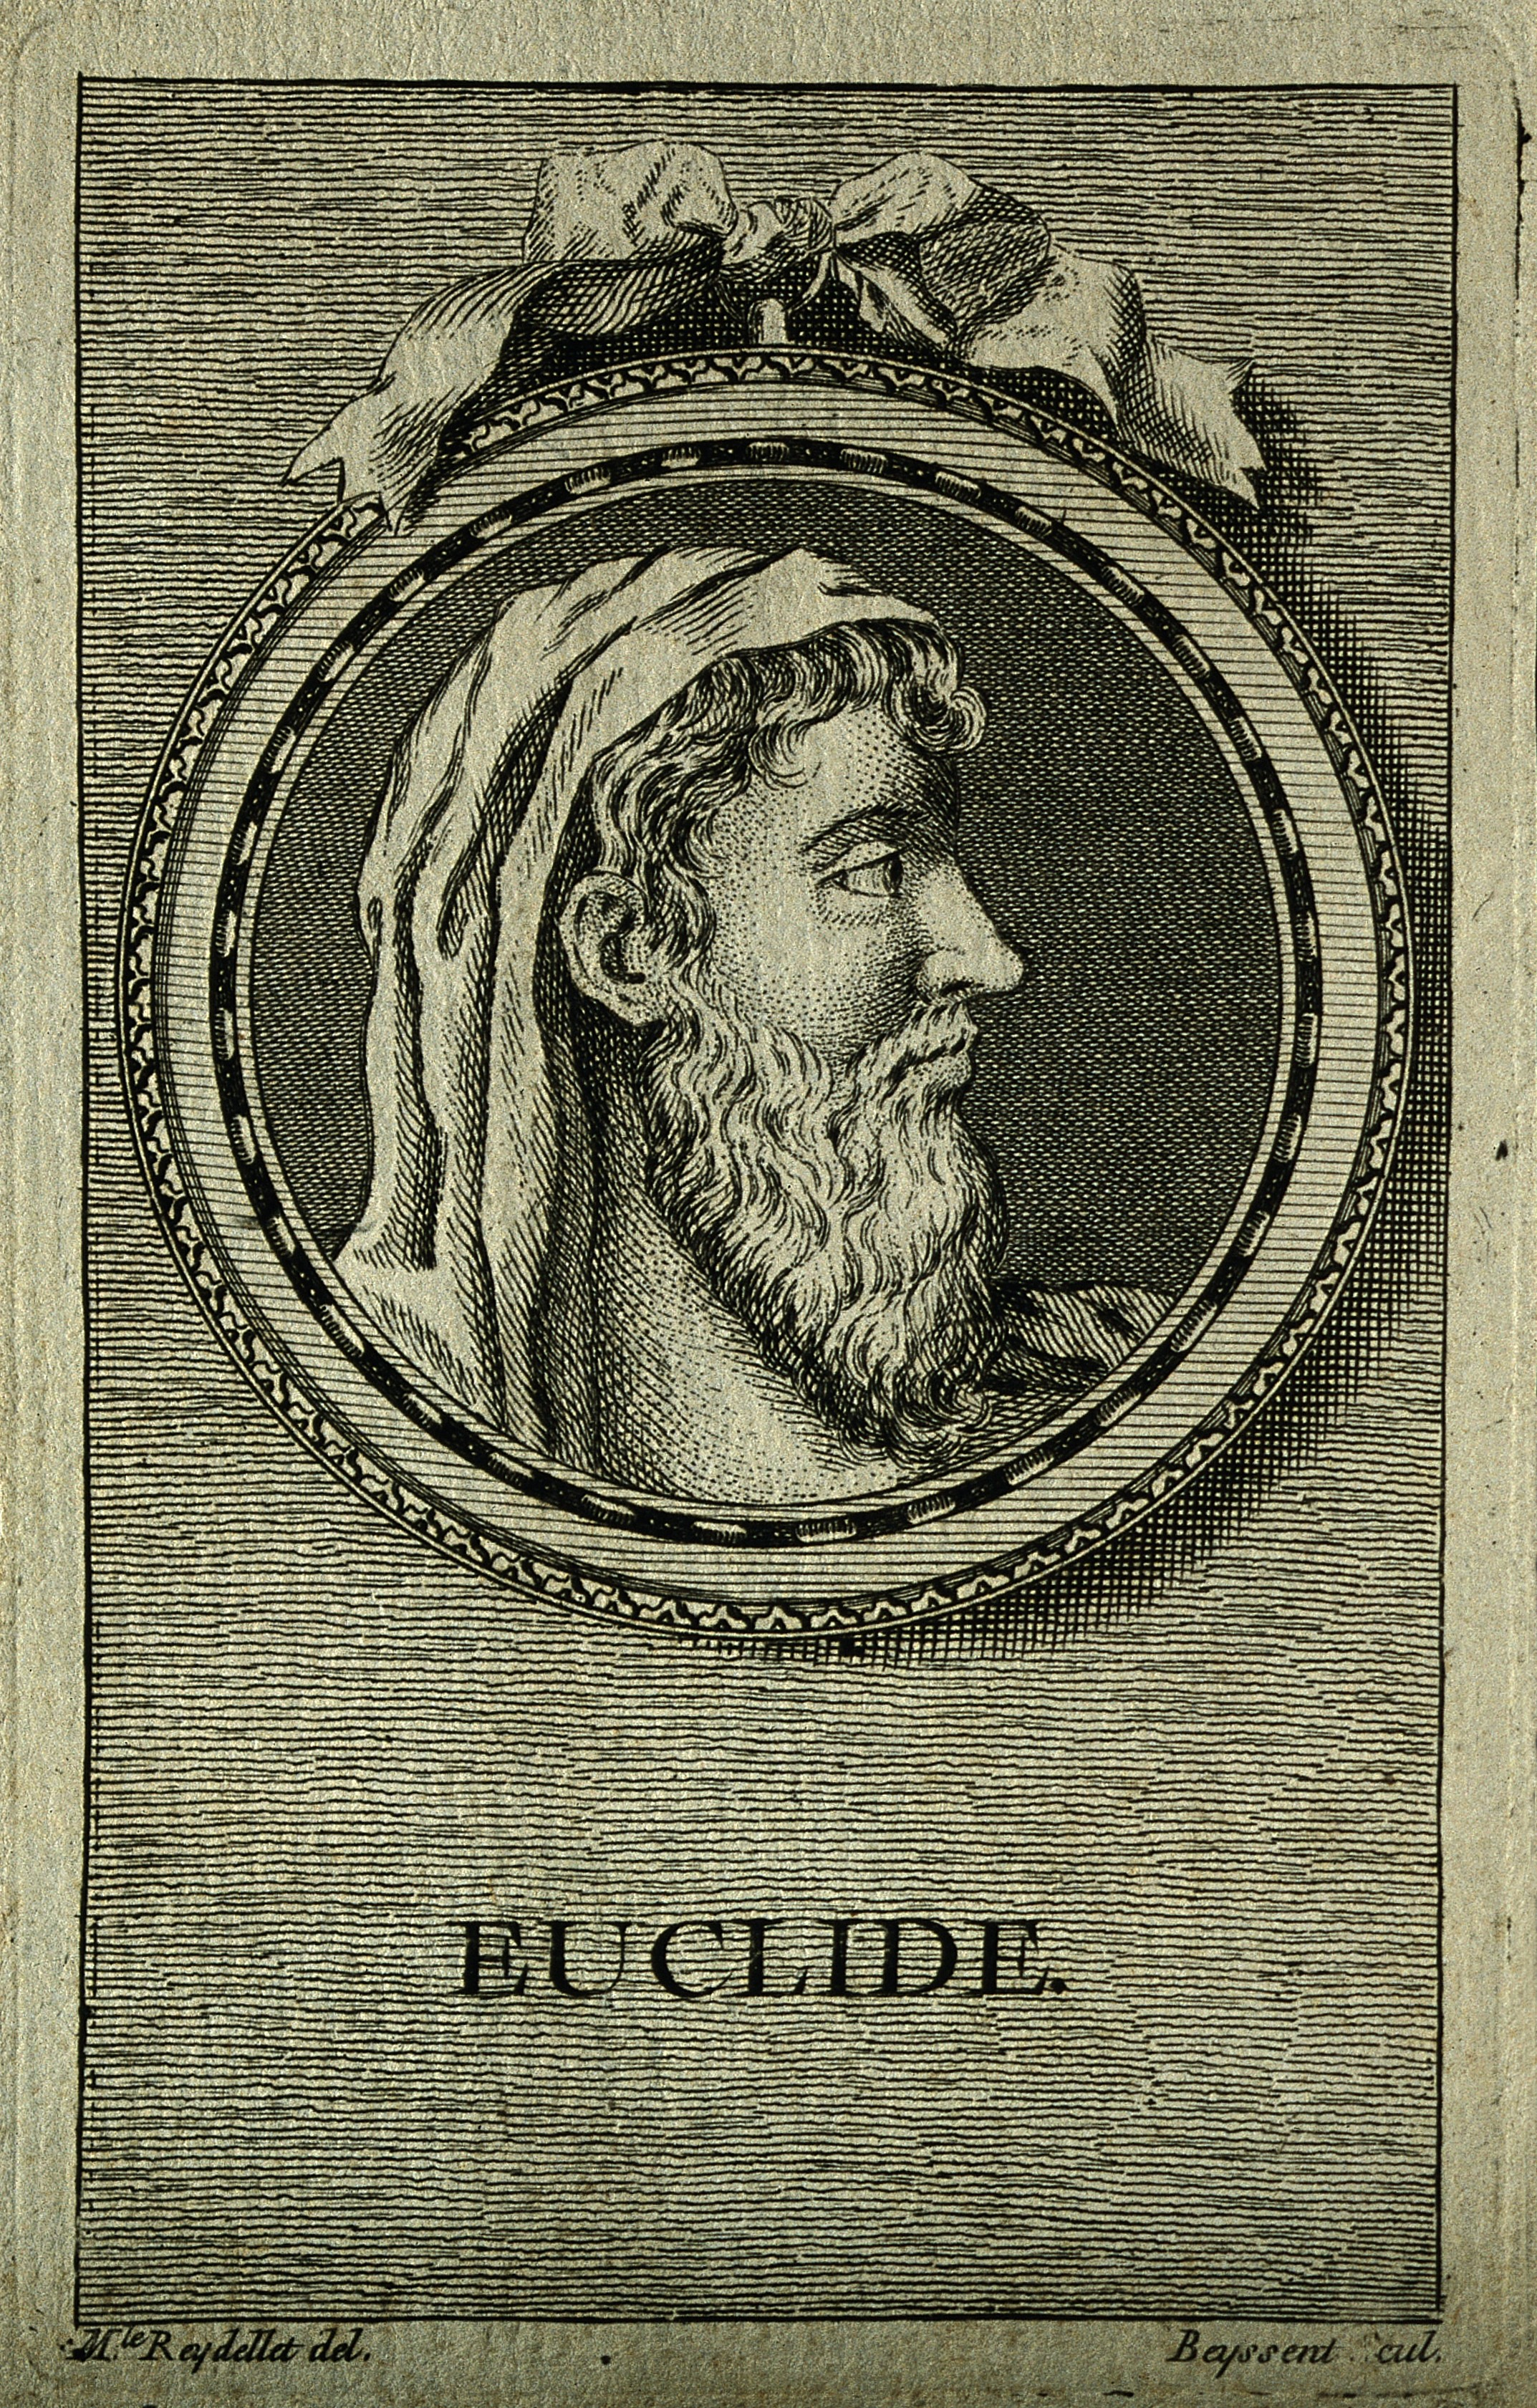
\includegraphics[
        alt={Portrait of Euclid of Alexandria.},
        height=\dimexpr.95\textheight-2pt\relax
      ]
      {figures/Euclid-Beyssent-line-engraving.jpg}%
    };
  \end{tikzpicture}
  \caption[Euclid of Alexandria]{\sloppy{Euclid of Alexandria. Line engraving by S. Beyssent after Mlle. C. Reydell.}}
  \label{figure:euclid}
\end{figure}

Number theory has a long history that dates back to antiquity. While a more complete history of mathematics would include findings about earlier civilizations \cite{boyer2011}, we begin our story in the Hellenistic city of Alexandria, which was founded by Alexander the Great in 331 BCE on the Mediterranean coast of Egypt. After the death of Alexander the Great in 323 BCE, Egypt came under the control of his general Ptolemy, who first ruled as satrap and became king of Egypt in 305/304 BCE \cite{fraser1972,holbl2001}. During the early Ptolemaic period, the city of Alexandria saw great development, such as the founding of the Mouseion, a state-supported research and teaching institution in which also the Library of Alexandria was housed \cite{casson2001}. This is the intellectual milieu in which Euclid of Alexandria likely lived, taught, and wrote one of the most influential manuscripts in the history of mathematics, the \textsc{Elements} \cite{euclid2015,heath1981}. In this monumental work, which is conventionally dated to around 300 BCE, Euclid systematically derived several key results in geometry and number theory from a small number of postulates. These include the infinitude of primes and the algorithm for finding the greatest common divisor, which bears his name. The 5\supth-century mathematical commentator Proclus reports in his commentary on Euclid's Elements that king Ptolemy came to Euclid with the question whether there is a quicker way of learning geometry \cite{proclus1992}. We can easily imagine the king recognizing the importance of Euclid's axiomatic approach but struggling with Euclid's careful derivations, and surely his royalty should not have to work through all thirteen books of the \textsc{Elements}. To which Euclid replied with the famous apothegm: \emph{"There are no royal roads to geometry."}

Around 250 CE, the Greek mathematician Diophantus of Alexandria wrote his \textsc{Arithmetica} \cite{diophantus1910}, which focused on solving equations with integer coefficients in one or multiple unknowns. This 13-volume work is often considered the first comprehensive treatment of algebra, though Diophantus relied on rhetorical descriptions rather than modern algebraic notation. Only six of the original volumes have survived, but they profoundly influenced later mathematicians.

The works of Euclid and Diophantus were preserved and studied by scholars in the Byzantine Empire, such as Theon of Alexandria and his daughter Hypatia. They added commentaries that clarified and expanded upon the original text.

During the Islamic Golden Age, scholars like Al-Khwarizmi, Ibn al-Haytham, and Omar Khayyam preserved and expanded upon the works of Euclid and Diophantus. Al-Khwarizmi's work, especially his \textsc{Kitab al-Mukhtasar fi Hisab al-Jabr wal-Muqabala} (from which the term "algebra" originates), introduced systematic methods for solving linear and quadratic equations. He used rhetorical algebra, like Diophantus, but began a transition toward symbolic representation by relying on consistent terminology for operations and equations.

After the invention of the printing press, Erhard Ratdolt, a German printer based in Venice, produced the first printed edition of the \textsc{Elements} in 1482. This edition included mathematical diagrams and marked an important step in the dissemination of Euclid's work. The first printed edition of Diophantus' \textsc{Arithmetica} was published in 1575 by Wilhelm Xylander, a German mathematician. The printing was done in Basel, Switzerland, which was a major hub for academic publishing at the time. By the time of Pierre de Fermat in the 17\supth{} century, both the \textsc{Elements} and \textsc{Arithmetica} had become essential texts for mathematicians across Europe, influencing the development of number theory and inspiring Fermat’s pioneering discoveries.

\subsection{Mathematics, Astronomy, and Poetry in Ancient India}

We could not move forward with the story of the greatest mathematical achievements without first turning our attention to the scholarly traditions of ancient India.

\subsection{Pierre de Fermat}

\begin{figure}[p]
  \centering
  \begin{tikzpicture}
    \node[inner sep=0pt, rounded corners=0.5em, clip] {%
      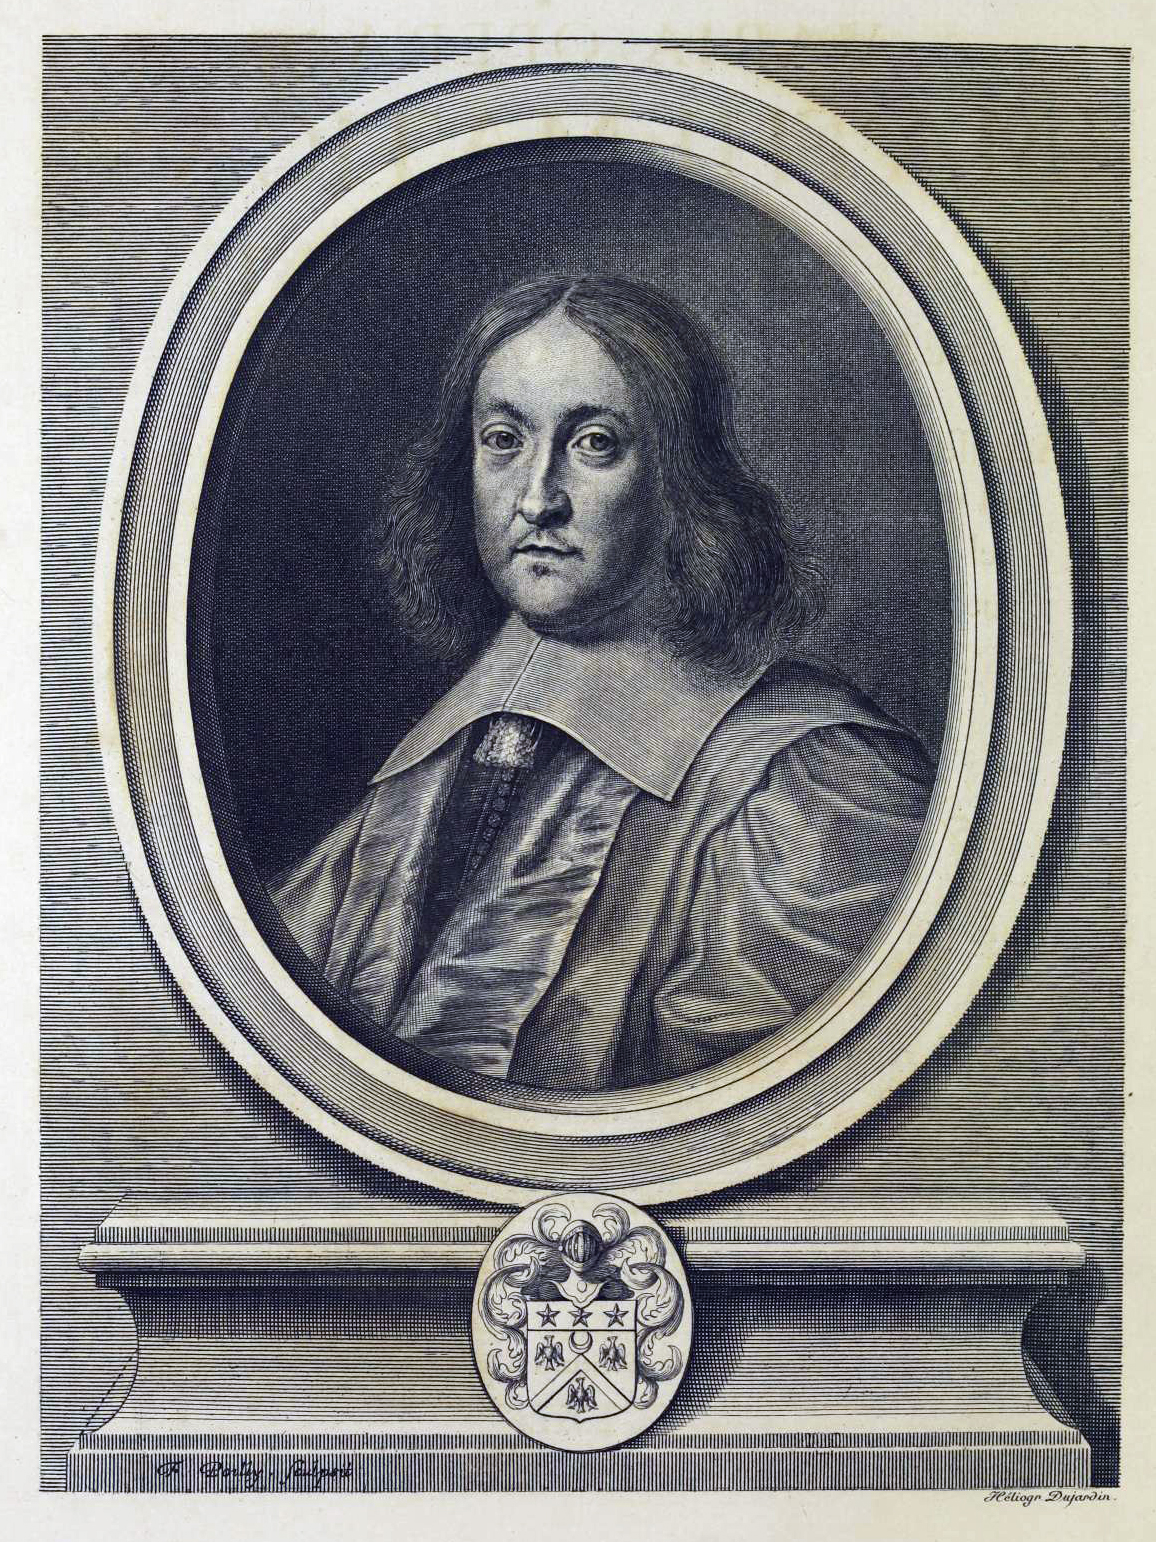
\includegraphics[
        alt={Portret of Pierre de Fermat.},
        height=\dimexpr.95\textheight-2pt\relax
      ]{figures/Fermat.jpg}%
    };
    \end{tikzpicture}
    \caption[Pierre de Fermat]{Pierre de Fermat. Engraving in Oeuvres Mathématiques Diverses.}
  \label{figure:fermat}
\end{figure}

Pierre de Fermat (1607--1665) is often considered the founder of modern number theory \cite{mahoney1994,weil1984}. He was a contemporary of Blaise Pascal and Marin Mersenne, both of whom he corresponded with, and also of Galileo Galilei. He wrote a manuscript titled \textsc{Éléments de Géométrie}, which served as an extension and commentary on Euclid’s \textsc{Elements}. In this work, he sought to modernize Euclid’s geometry by applying the emerging methods of algebra and analytic geometry to classical geometric problems.

Fermat made many groundbreaking discoveries in the theory of numbers. Among his most influential discoveries is \emph{Fermat's Little Theorem}, which states that if $p$ is a prime number, then
\begin{equation*}
  a^p\equiv a\pmod{p}.  
\end{equation*}
This theorem is key to many further results in modular arithmetic, and has modern applications in RSA encryption. Fermat also came up with the method of \emph{infinite descent}, which allows one to show that a certain equation or proposition cannot hold by showing that it would lead to an infinite descending sequence of positive integers. Fermat was very fond of this method, and used it brilliantly to prove some of his most profound claims. For instance, the case $n=4$ of \emph{Fermat's Last Theorem}, which states that there are no positive integers $x$, $y$, and $z$ such that $x^4+y^4=z^4$ is proven using infinite descent. In order to prove this fact, Fermat also showed that the area of a Pythagorean triangle is never a perfect square. Fermat is furthermore famous for the \emph{Two-Squares Theorem}, which states that any prime $p\equiv 1\pmod{4}$ can be written uniquely as a sum of two squares, and that primes $p\equiv 3\pmod{4}$ cannot be written as a sum of two squares. Fermat also claimed that any number can be written as the sum of at most three triangular numbers, as the sum of four squares, as the sum of five pentagonal numbers, and so on, but he did not indicate how these claims might be proven. The case of the triangular numbers is now known as Gauss's \emph{Eureka Theorem}, the \emph{Four-Squares} theorem was proven by Lagrange, and Cauchy proved the general theorem asserting that any number can be expressed as the sum of at most $n$ $n$-gonal numbers.

Fermat also made several famous conjectures. He conjectured that the equation $x^2+Ny^2=1$ has infinitely many solutions for any non-square integer $N$. Euler made a significant advance to this problem by proving it for specific values of $N$. The general form of the solution to equations of the form $x^2+Ny^2=1$ was found later by Legendre and Lagrange.

Finally, Fermat famously asserted that there could be no three positive integers $x$, $y$, and $z$ such that the equation
\begin{equation*}
  x^n+y^n=z^n
\end{equation*}
holds, when $n\geq 3$. This statement is now known as \emph{Fermat's Last Theorem}. He claimed to have a "truly marvelous proof", but that the margin of his copy of \textsc{Arithmetica} was too small to contain it. His assertion, known as \emph{Fermat's Last Theorem}, captivated mathematicians for centuries. It was finally proven in 1995 by Andrew Wiles, about 350 years after Fermat made his famous note in the margin, using advanced techniques from algebraic geometry and modular forms. Wiles’s achievement is considered one of the most remarkable milestones in the history of mathematics.

\subsection{Leonhard Euler}

\begin{figure}[p]
  \centering
  \begin{tikzpicture}
    \node[inner sep=0pt, rounded corners=0.5em, clip] {%
      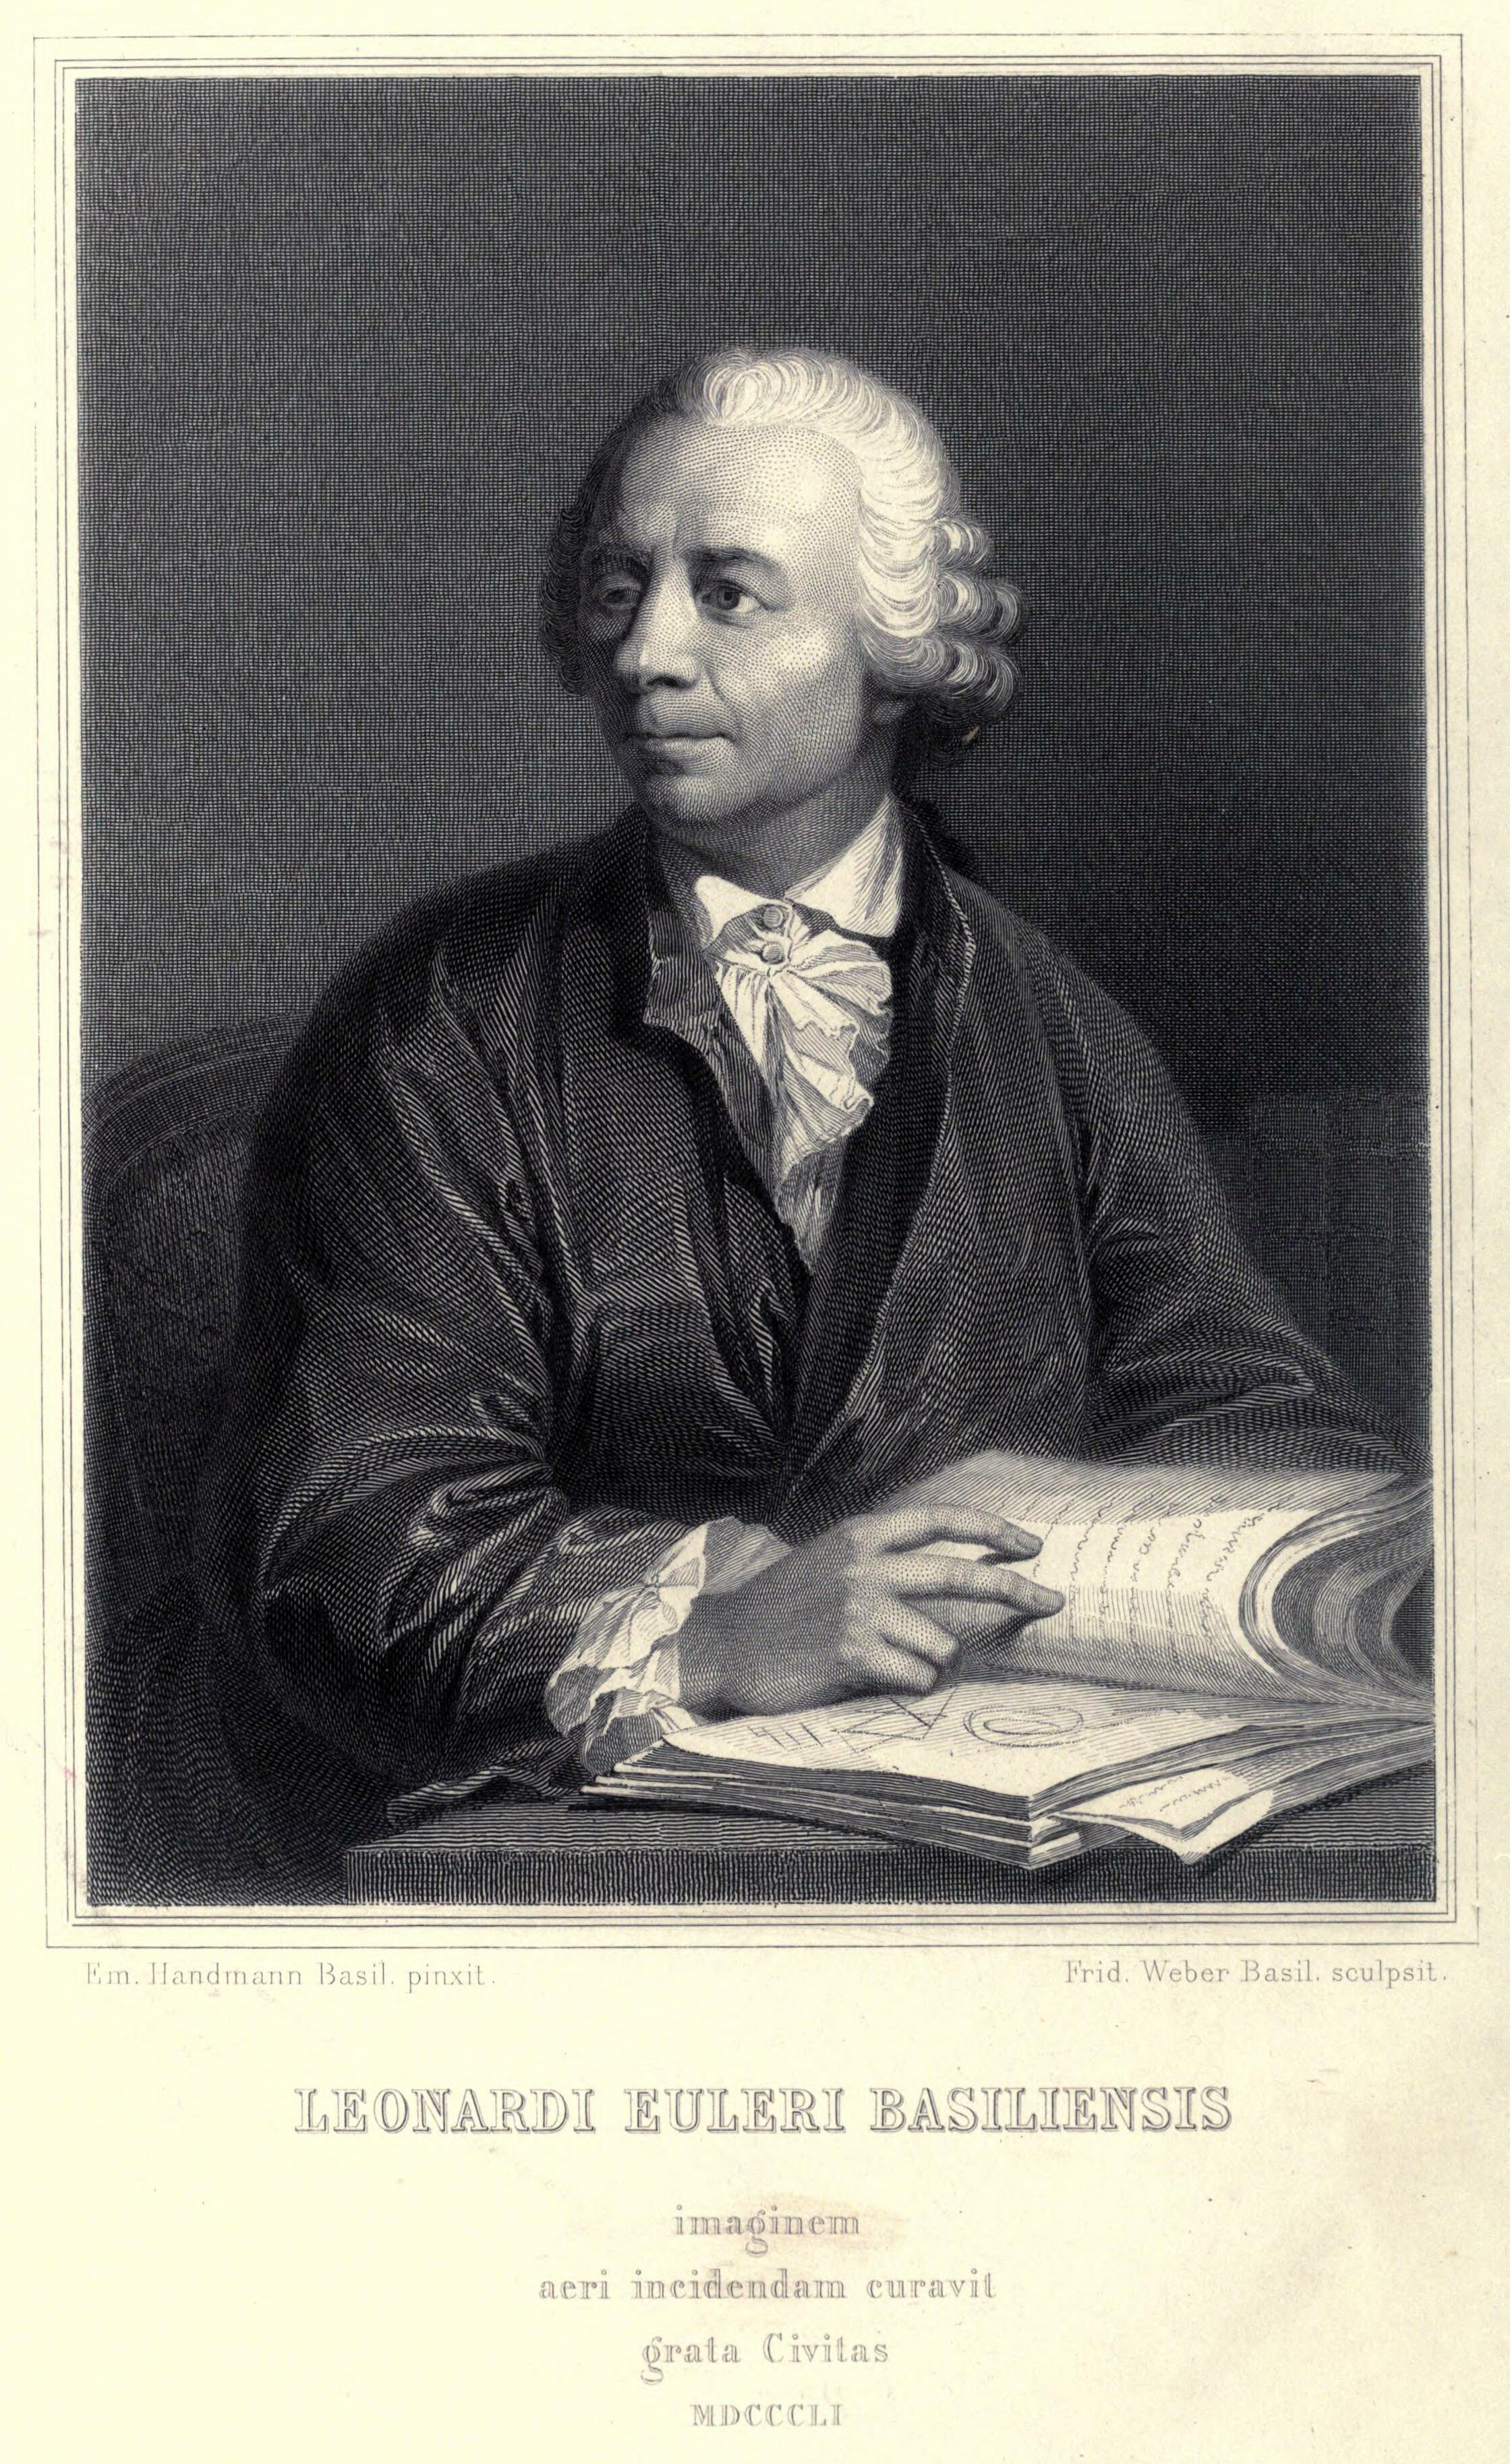
\includegraphics[
        alt={Portrait of Leonhard Euler.},
        height=\dimexpr.95\textheight-2pt\relax
      ]
      {figures/Euler.jpg}%
    };
  \end{tikzpicture}
  \caption[Leonhard Euler]{Leonhard Euler. Engraving by Friedrich Weber.}
  \label{figure:euler}
\end{figure}
While Fermat laid the groundwork for modern number theory, we should mention that the concept of \emph{function} hasn't been crystallized until Leibniz coined the term in 1673, using it to describe quantities related to curves, such as slopes, tangents, and areas. Bernoulli played a significant role in expanding the idea of functions.
He used the term explicitly in 1718, describing it as a quantity dependent on another variable. Euler provided the first modern definition of a function in his \textsc{Introductio in Analysin Infinitorum} (1748) \cite{euler1988}.
He emphasized that functions could include both algebraic (e.g., polynomials) and transcendental forms (e.g., trigonometric and exponential functions). Peter Gustav Lejeune Dirichlet was the first to define functions abstractly as a correspondence between two sets, removing the requirement for expressions or formulas.
This abstraction was a key insight for the theorem that we now know as \emph{Dirichlet's theorem}: Every arithmetic progression
\begin{equation*}
  a,\ a+b,\ a+2b,\ a+3b,\ \ldots
\end{equation*}
in which $a$ and $b$ are coprime, contains an infinitude of primes. Dirichlet proved his theorem in 1837, more than 150 years after Leibniz first coined the term of function.

Euler's Introductio in Analysin Infinitorum marked the beginning of \emph{analytical number theory}. As we mentioned before, Euler defined functions here and established the notation $f(x)$ of a function applied to its variable, which we still use today. He derived the famous formula for complex exponentials
\begin{equation*}
  e^{ix}=\cos(x) + i \sin(x).
\end{equation*}
This identity connects the exponential function, trigonometric functions, and the imaginary unit. The Riemann zeta function $\zeta(s)$ makes its first appearance here in a complex variable $s$, and he derived the celebrated \emph{product formula}
\begin{equation*}
  \zeta(s)=\sum_{n=1}^{\infty}\frac{1}{n^s}=\prod_{p\,\mathrm{prime}}\frac{1}{1-p^{-s}}.
\end{equation*}
More generally, Euler explored infinite series and products. The \emph{Basel summation formula}
\begin{equation*}
  \sum_{n=1}^\infty \frac{1}{n^2}=\frac{\pi^2}{6}
\end{equation*}
was first proven here, which was one of Euler's most celebrated achievements. Euler was keen to explore the connection between geometry and analysis, and in Introductio in Analysin Infinitorum, he advanced the idea that the study of functions and infinite series could provide new insights into geometric problems. He showed how techniques from analysis could be used to solve problems in geometry and vice versa, fostering the development of applied mathematics.

\subsection{Johannes Carl Friedrich Gauss}

\begin{figure}[p]
  \centering
  \begin{tikzpicture}
    \node[inner sep=0pt, rounded corners=0.5em, clip] {%
      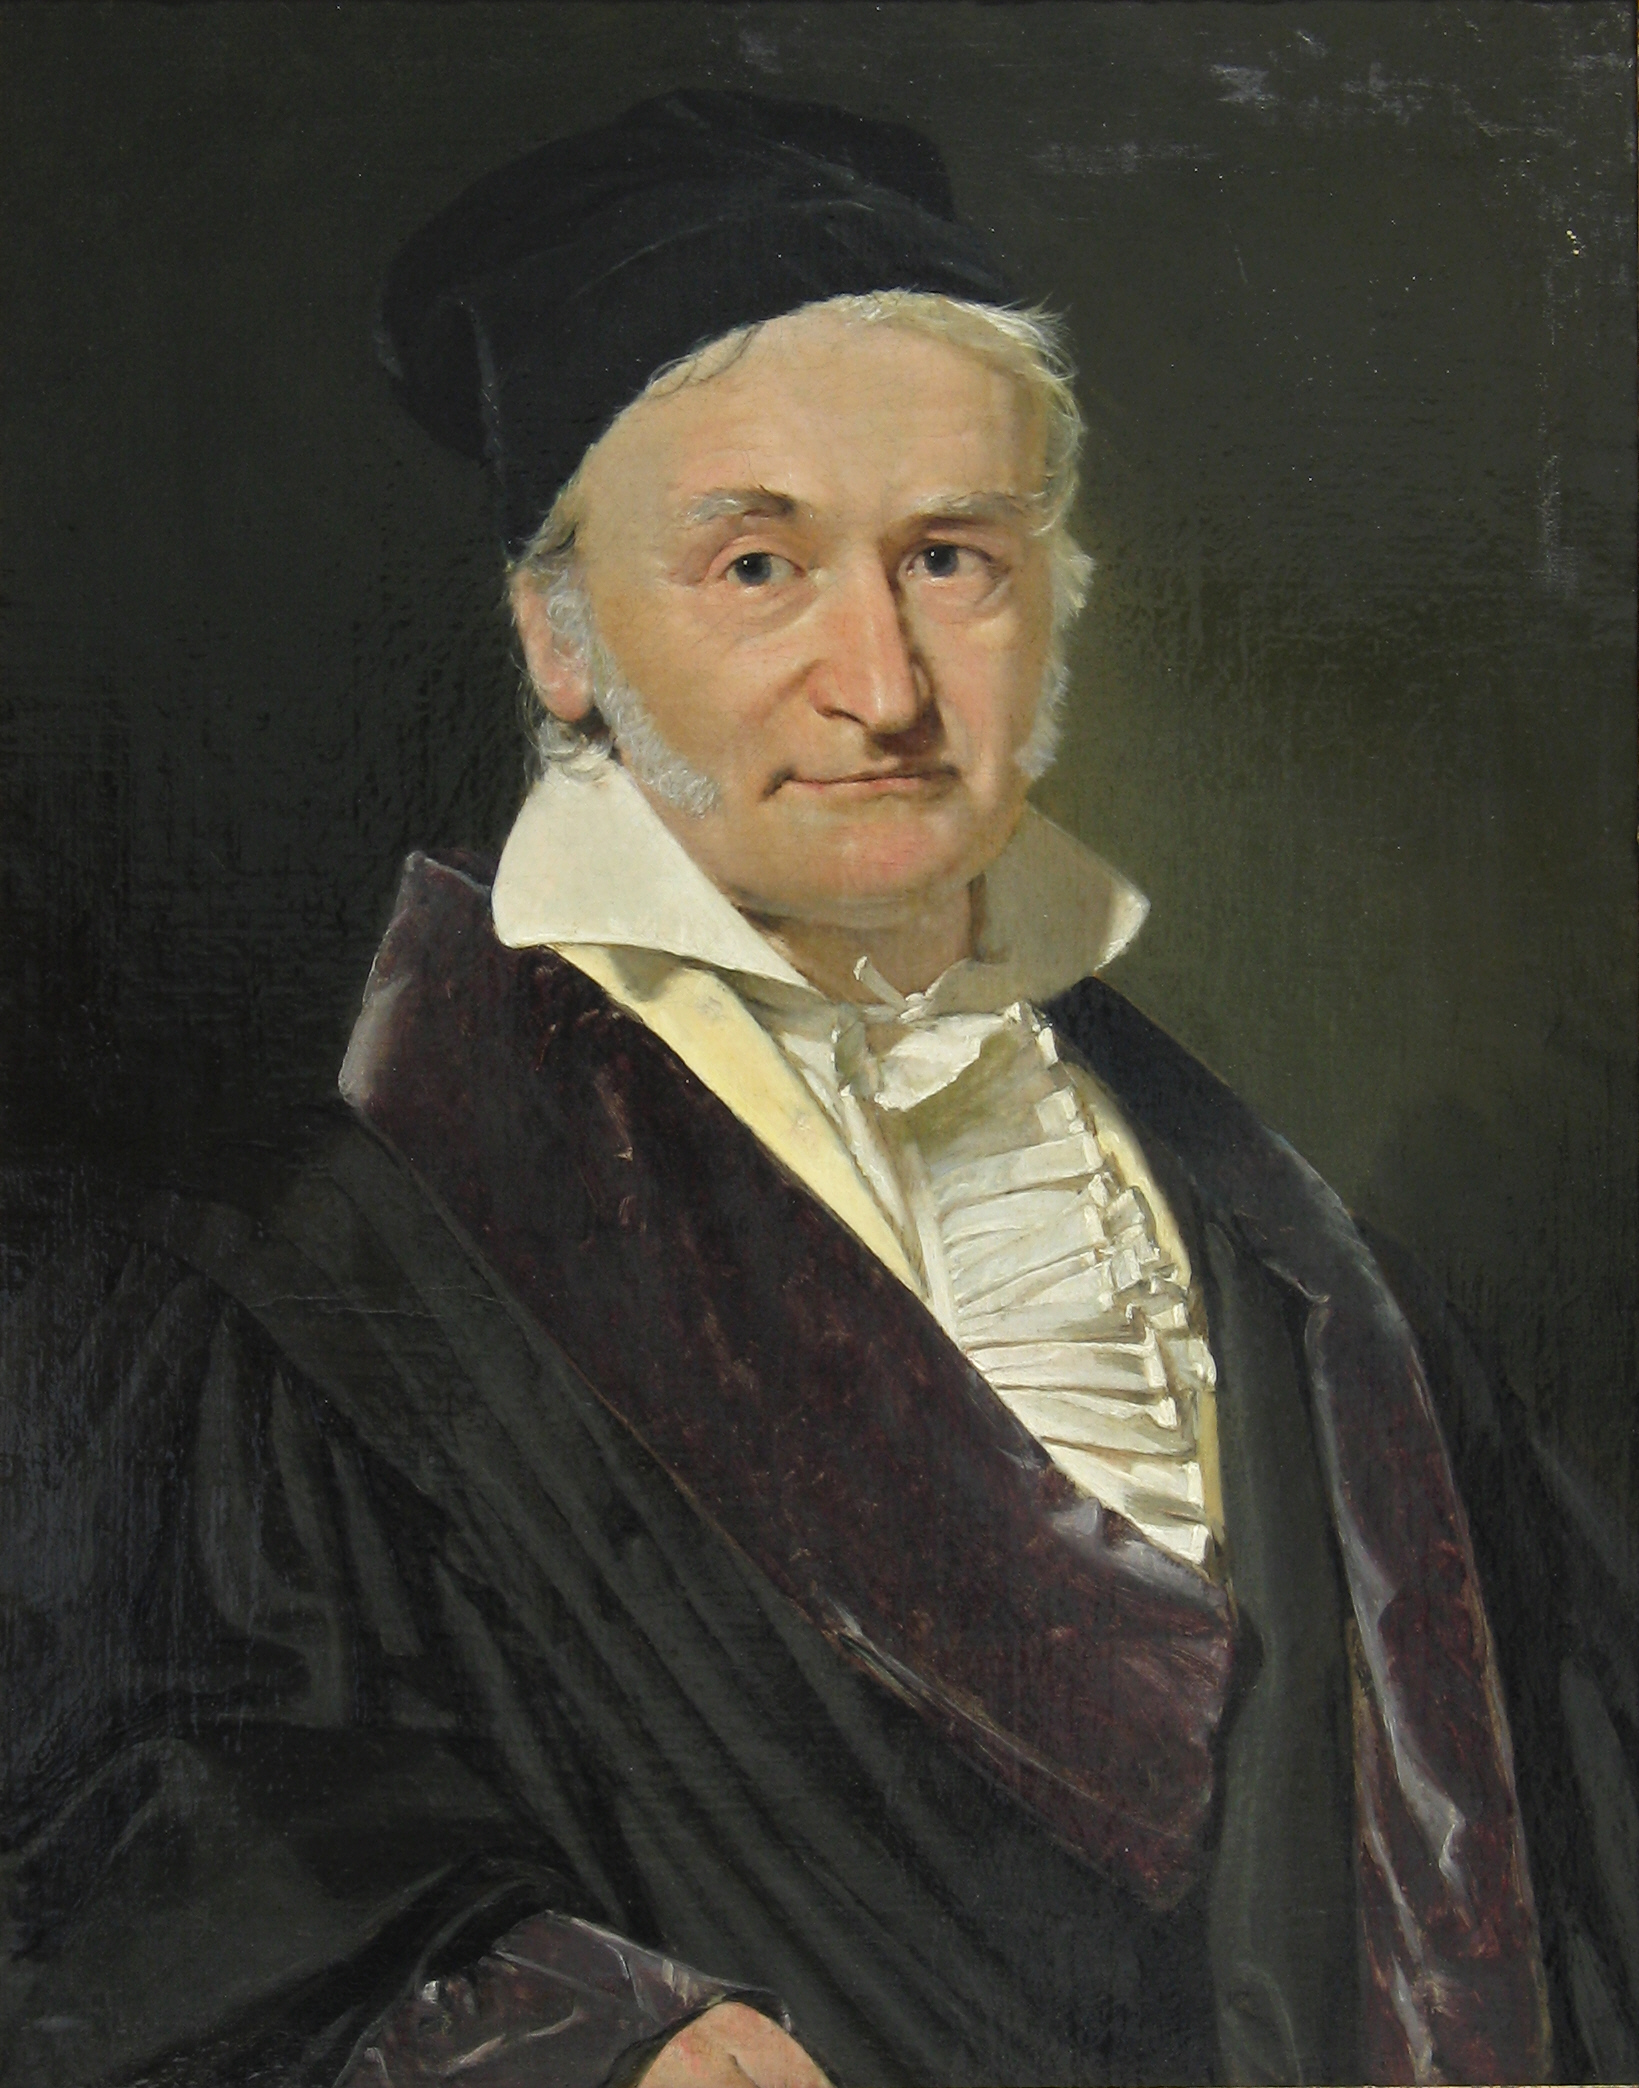
\includegraphics[
        alt={Portret of Carl Friedrich Gauss.},
        height=\dimexpr.95\textheight-2pt\relax
      ]
      {figures/Gauss.jpg}%
    };
  \end{tikzpicture}
  \caption[Carl Friedrich Gauss]{\sloppy{Carl Friedrich Gauss. Painting by Christian Albrecht Jensen.}}
  \label{figure:gauss}
\end{figure}
Building on the work of Euler, Gauss began using the properties of the zeta function and other analytic methods to investigate the distribution of the primes. His seminal work \textsc{Disquisitiones Arithmeticae} \cite{gauss1986} is often considered the starting point of the study of the distribution of primes, ultimately leading up to the \emph{Prime Number Theorem}. Gauss conjectured that the number $\pi(n)$ of primes below a number $n$ satisfies the asymptotic law
\begin{equation*}
  \pi(n)\sim\frac{n}{\log(n)}.
\end{equation*}
This conjecture was proved independently by Jacques Hadamard and Charles Jean de la Vallée Poussin. Furthermore, Gauss laid the foundation for modular arithmetic, and proved the celebrated law of quadratic reciprocity, which tells us when a quadratic equation modulo a prime number is solvable. More precisely, it states that if $q\equiv 1\pmod{4}$ then the congruence $x^2\equiv p \pmod{q}$ is solvable if and only if the congruence $x^2\equiv q\pmod{p}$ is solvable.

A brief remark on the interesting etymology of the word theorem is in order. The English word \emph{theorem} ultimately derives from the Ancient Greek {\greekfont θεώρημα} (the\={o}r\={e}ma), literally “that which is seen”, and by usage in classical philosophy as an “object of contemplation”. The verb {\greekfont θεωρεῖν} (\emph{theōreîn}, “to observe, examine”) and the agent noun {\greekfont θεωρός} (\emph{theōrós}, “spectator”) are close relatives, and ultimately give us both `theorem' and `theory'.

In Euclid's \textsc{Elements}, specifically through the careful editorial work and commentaries of the Byzantine scribes, we start seeing the label \emph{theōrēma} for statements that require deductive proof, in contrast to the “givens” ({\greekfont ὑπόθεσις}, hypóthesis) and “proof” ({\greekfont ἀπόδειξις}, apódeixis). However, the fixed label \emph{Theōrēma} for such statements emerges more clearly in Medieval translations into Late Latin and Middle French of the \textsc{Elements}, through the editorial adjustments made by his copyists. The Late Latin word \emph{theorema} and the Middle French word \emph{théorème} both retained the meaning “proposition that is to be proved”.

Euclid's \textsc{Elements} was first translated into English by Sir Henry Billingsley in 1570, who was mayor of London at the time, with a preface written by John Dee. This Billingsley--Dee edition of Euclid’s \textsc{Elements} established \emph{theorem} in the English language as a word meaning “proposition that is to be proved”. Over the ensuing centuries, the word theorem came to mean exclusively a mathematical assertion proven from axioms, definitions, and previously established theorems.

\subsection{Contemporary Mathematics}

So far, we have covered some of the most celebrated advances in humanity's understanding of numbers up to the early 19\supth{} century. Mathematics has made rapid progress since then. Bertrand's postulate, which asserts that there is always at least one prime $p$ between $n$ and $2n$, for any $n>1$, was proven by Pafnuty Chebyshev in 1852, and Ben Green and Terence Tau proved in 2004 that the sequence of prime numbers contains arbitrarily long arithmetic progressions.

The 20\supth{} century saw the emergence of the Langlands program, a far-reaching research program that aims to connect number theory, representation theory, and algebraic geometry. With the contributions of mathematicians like André Weil, Robert Langlands, and many others, the program has shaped much of the direction of modern research in number theory and its applications to other branches of mathematics.

Even today fundamental concepts such as sets and functions continue to evolve. We live in an era of digital computation, with tools far beyond the reach of Fermat, Euler, and Gauss, where essentially all recorded knowledge is readily available to almost anyone. This computational revolution has also given rise to powerful tools like proof assistants; that is, computer programs designed to construct and formally verify mathematical proofs. Since proof assistants are programming languages, they are often based on type theory rather than set theory, slightly changing the way mathematics is done. Functions in type theory are even more general than Leibniz, Euler, and Dirichlet envisioned: unlike in set theory where functions are a specific kind of relations between sets, functions in type theory are primitive entities satisfying certain rules for evaluation, and they have an extra dependency built in, allowing types of their outputs to depend on the input. Proof assistants are being used with great success to formally verify advanced mathematical theorems. Georges Gonthier formally verified the Four Color Theorem and the Odd Order Theorem, and Tom Hales verified Kepler's conjecture about sphere packings. A current effort led by Kevin Buzzard aims to formally verify Fermat's Last Theorem.

Today, number theory continues to be one of the most active and fruitful areas of mathematical research, all of which started simply with counting on ten fingers.

\section{The Concept of Number Through History}

Many people are familiar with numbers through everyday experiences like counting, measuring, or comparing quantities. From a young age, we develop an intuition about how numbers behave. Our experience with numbers reveals patterns and properties that seem to always be true. For example, we quickly learn that it does not matter in which order we add two numbers: Given two numbers $a$ and $b$ it is always true that $a+b=b+a$. Truths such as this one seem so self-evident that we might be tempted to just accept them. However, for a rigorous mathematical theory we need to be more careful. Mathematicians require proofs. Checking a property for every number up to a hundred, a million, or even $10^{27}$ might confirm a pattern, but infinitely many numbers remain beyond such finite checks. Mathematical proofs, on the other hand, are logical arguments that establish beyond any possibility of doubt why certain properties hold universally for all numbers, or at least for precisely defined sets of numbers. To reason about all natural numbers at once, we need formal principles that extend beyond empirical observation and anecdotal evidence. In order to discover such reasoning principles, we need to find out first what the natural numbers really are, a question with a rich and very interesting history.

% Clarify that Nicomachus lived around 100 CE, while Euclid lived around 300 BCE, implying that the transition used from the Pythagorean school of thought to Euclid's school of thought might not be historically accurate.

Although natural numbers arise from counting, the notion of number is not inherently linked to any particular collection of entities being counted. Scholars in the Pythagorean tradition were among the first to articulate this insight. Nicomachus emphasized in his \textsc{Introduction to Arithmetic} the concepts of \emph{monad} and \emph{dyad} for the totality of all things that come in one or two units \cite{nicomachus1926}. Nicomachus ascribed divine properties to the monad, or unity: ``{\itshape It generates itself without beginning, without end, and appears to be the cause of enduring, as God in the realm of physical actualities is in such manner perceived of as a preserving and guarding agent of nature}''. Nicomachus drew strong parallels between the monad and the concept of sameness, and dually between the dyad and the concept of otherness. He also emphasized that numbers were composed of monads. In other words, the monad is the source of all numbers. Although mathematicians do not ascribe divine properties to numbers anymore, we see here the emergence of some important ideas. The first is that all numbers are generated from the monad, that is, unity. The second idea is to connect unity with sameness. The idea that all things equal to a given object form a unit, or a singleton, anticipates a fundamental principle of equality. However, we shall forego the interesting digressions that we could make about equality and focus our attention on the concept of number.

Euclid takes a more abstract point of view, in which the concept of number is defined without relating it to the divine conception of the monad. For Euclid, a \emph{unit} is the conceptual principle by which an individual object is identified as one, and a \emph{number} is a multitude composed of such units in a discrete fashion \cite{euclid2015}. In other words, the concept of unit captures the notion of oneness, but this is distinct of the number $1$ itself. Both Nicomachus's and Euclid's views on the concept of number were highly influential throughout late antiquity and the Middle Ages, particularly through Boethius's Latin rendition of Nicomachus's \textsc{Introduction to Arithmetic} \cite{kaylorphillips2012} and Adelard of Bath's translation of Euclid's \textsc{Elements} \cite{clagett1953}.

While Pierre de Fermat is regarded the founder of modern number theory, he did not write extensively on the philosophy of mathematics. Nevertheless, certain themes in his correspondence and work show a clear orientation. For him, mathematics is about truths intrinsic to numbers. Numbers were the object of exact reasoning. He emphasized that \emph{induction}, by which mathematicians up to the early 19\supth{} century understood experimental verification, was insufficient to establish universal truths of numbers. Nowadays, this historical use of the word induction is sometimes called \emph{empirical induction}. Among Fermat's lasting contributions was his method of infinite descent, a method of proof by contradiction in which one shows that any supposed solution would lead to an ever-decreasing sequence of natural numbers, which is impossible.

With Euler, we witness a significant conceptual expansion. In his \textsc{Elements of Algebra}, Euler extended the notion of number beyond the natural and rational to encompass negative numbers, irrationals, complex numbers, and even infinite series. He was among the first to conjecture that constants like $e$ and $\pi$ are transcendental; that is, not the roots of any algebraic equation with rational coefficients. For Euler, numbers were entities governed by formal laws, irrespective of whether they corresponded to geometric magnitudes. Euler's broadening of the concept of numbers, and his use of analytic methods would eventually spark debates about the foundations of mathematics and the logical principles underlying mathematical truth.

In the 19\supth{} century, the nature of mathematics itself began to change. The emergence of non-Euclidean geometry was a challenge to the status of Euclid's Elements as the de facto foundation of mathematics, and Weierstrass's discovery of continuous, nowhere differentiable functions meant that one could not simply rely on intuition in the study of calculus and analytics. Furthermore, with Galois's use of symmetries in order to show that quintic equations had no solutions expressible in terms of radicals, abstract algebra became a prominent subject of mathematics with algebraic objects that have little in common with numbers except for a few formal laws. These discoveries underscored the need for a more solid foundation of mathematics, ultimately resulting in the emergence of Frege's logicism and set theory.

Nevertheless, the question of formally defining the set of natural numbers was left mostly unexplored until the second half of the 19\supth{} century. Even as late as 1886, Kronecker is quoted as proclaiming that ``God created the integers, all else is human work'' \cite{weber1893}, not helping the cause of finding a definition of the natural numbers. In \emph{Was sind und sollen die Zahlen?} (translated to English as \emph{What are numbers and what should they be?}), Dedekind was the first to formally define the set of natural numbers. His idea was that the number zero and the successor function together should be sufficient to describe all the natural numbers. He formalized this idea in 1888 by specifying that the set of natural numbers is a \emph{simply infinite set}, meaning that there is a one-to-one function $S:\mathbb{N}\to\mathbb{N}$ such that every element of $\mathbb{N}$ can be reached by iteratively applying $S$ to an element $0$, which is not itself a value of $S$ \cite{dedekind1888}. Dedekind showed furthermore that all simply infinite sets are similar to each other; in modern termimology, he showed that all simply infinite sets are \emph{isomorphic}. Thus, Dedekind's definition was structural in nature, in the sense that it captured the structure a set must possess in order for it to be considered a set of natural numbers.

Not much later, Giuseppe Peano arrives at a very similar definition of the set of natural numbers. In \textsc{Arithmetices principia nova methodo exposita} he established the set of natural numbers as a set satisfying a small number of axioms, the celebrated \emph{Peano axioms} \cite{peano1889}:
\begin{enumerate}
\item For any two natural numbers $x$ and $y$ we have
  \begin{equation*}
    (x=y)\Leftrightarrow (S(x)=S(y)).
  \end{equation*}
\item There is no natural number $x$ such that $S(x)=0$.
\item For any set $A$, if $0\in A$ and if for any natural number $x$ we have $(x\in A) \Rightarrow (S(x)\in A)$, then every natural number is in $A$.
\end{enumerate}
The first axiom establishes that the successor function $S$ is one-to-one. This means that every natural number is the successor of at most one natural number. The number $0$ itself is, in the setup of Dedekind and Peano, not a successor by the second axiom. The third axiom encodes \emph{mathematical induction}. The notation $x\in A$ means that $x$ is an element of $A$, or in other words that $A$ contains the element $x$. Thus, Peano's third axiom asserts that if $A$ is a set containing $0$ and containing the successor of every element it contains, then it contains all the natural numbers. While the similarity between Dedekind's and Peano's approach is clear, we note Dedekind's approach was structural, set-theoretic, and intended for a philosophical audience, Peano's approach was formal, logical, and symbolic.

A common alternative way of formulating mathematical induction is as follows. Given any property $P(n)$ expressing a condition of an arbitrary natural number $n$, in order to prove that $P(n)$ is true for all $n$ it suffices to prove that:
\begin{enumerate}
\item The property $P(0)$ is true.
\item For all $n$, if the property $P(n)$ holds then the property $P(n+1)$ holds.
\end{enumerate}
Mathematical induction formalizes the idea that every natural number is either $0$ or it is the successor of a previous natural number. Proving a property for all natural numbers therefore breaks down in two cases: The \define{base case} in which we prove that $P(0)$ is true, and the \define{inductive step} where we prove that $P(n+1)$ is true provided that $P(n)$ is true.

While proofs by mathematical induction go back to antiquity, the first to formulate the mathematical induction abstractly as a method of proof was Blaise Pascal in his \textsc{Traité du triangle arithmétique} \cite{pascal1665}. In this work, he studied the triangle of numbers now named after him. In a passage on the ratios of two horizontally adjacent binomial coefficients he wrote:
\begin{quote}
  {\itshape
    Quoy que cette proposition ait une infinité de cas, j'en donneray une démonstration bien courte, en supposant deux lemmes.
    
    Le 1.~qui est évident de soy-mesme, que cette proportion se rencontre dans la seconde base; car il est bien visible que φ est à σ comme 1 à 1.
    
    Le 2.~que si cette proportion se trouve dans une base quelconque, elle se trouvera nécessairement dans la base suivante.  
  }
\end{quote}
Notice, however, that Pascal did not yet use the term \emph{induction} for this method of proof. As we mentioned earlier, mathematicians of his time understood the word induction to refer to the empirical method of extrapolating patterns from finite data. Augustus De Morgan was the first to coin the term \emph{mathematical induction} in 1838, albeit somewhat incidentally \cite{cajori1918}. In his article on this topic in the \textsc{Penny Cyclopedia} he coined the term \emph{successive induction}, but he used the phrase \emph{mathematical induction} in a concluding remark \cite{demorgan1838}. Through the efforts of Dedekind and Peano, the induction principle has evolved from a method of proof to a defining principle for the set of natural numbers. 

By the turn of the 20\supth{} century, set theory, as pioneered by Georg Cantor and developed further by Richard Dedekind and others, was increasingly seen as a promising foundation for mathematics. However, the emergence of paradoxes around 1900 prompted efforts to axiomatize set theory. Beginning with Zermelo's axioms in 1908 and refined into the Zermelo--Fraenkel system in the 1920s, set theory gradually became the de facto foundational framework for modern mathematics. This raises the question whether the natural numbers can be defined within Zermelo--Fraenkel's set theory. Von Neumann gave an elegant set-theoretic definition of the natural numbers: The number $0$ was defined as the empty set $\varnothing$, the number $1$ was defined as the set $\{0\}$ containing the empty set, the number $2$ was defined as the set $\{0,1\}$, and so on:
\begin{equation*}
  0:=\varnothing,\qquad 1:=\{\varnothing\},\qquad 2:=\{\varnothing,\{\varnothing\}\}\qquad 3:=\{\varnothing,\{\varnothing\},\{\varnothing,\{\varnothing\}\}\},\qquad\ldots
\end{equation*}
However, Von Neumann's definition is not the only possible definition. One can also define
\begin{equation*}
  0:=\varnothing,\qquad 1=\{\varnothing\}, \qquad 2:=\{\{\varnothing\}\},\qquad 3 := \{\{\{\varnothing\}\}\},\qquad\ldots
\end{equation*}
These two definitions are clearly distinct, since $0\in 2$ is true in Von Neumann's definition but false in the latter definition. This raises the question, if Zermelo--Fraenkel set theory is to be the foundation of mathematics, then what is \emph{the} set of natural numbers? Paul Benacerraf argued in his famous essay \emph{What numbers could not be?} that the essence of the set of natural numbers is its structure, much like Dedekind had already argued almost a century before him \cite{benacerraf1965}.

While mathematicians often prefer to work with sets, computer scientists might prefer to work with types.  The distinction is merely that of the logical framework being used: Most mathematicians rely on the Zermelo--Fraenkel set theory, while computer scientist rely on programming languages that often have a type theory in its foundation. Theorem proving in computer programs called \emph{proof assistants} is rapidly becoming a more essential mathematical activity for students and researchers alike. However, many of the most popular proof assistants are based on type theory, in which collections of mathematical objects are called types.

Modern mathematics is increasingly formalized in computer programs called \emph{proof assistants}. There are many libraries of formalized mathematics in active current development, containing vast amounts of mathematics from a wide variety of mathematical subjects. However, the foundation of most such systems is not set-theoretic. Instead, many proof assistants use \emph{dependent type theory} as their foundational language, which was developed in the 1970s and 80s by Per Martin-L\"of. Both sets and types are collections of abstract objects often referred to as \define{elements}, but the formalisms by which they are studied are different in character, thus justifying the different names \emph{sets} and \emph{types}. The way the natural numbers are introduced in type theory is also slightly different. Whereas the induction principles of Dedekind and Peano establish the inclusion of the set of natural numbers into other sets, the natural numbers in type theory come equipped with a \emph{structural induction principle} that allows one to define functions out of the natural numbers. Similar to the previous definitions, the type of natural numbers comes equipped with $0$ and a successor function. The structural induction principle states that in order to define a function $f(n)$ taking as input a natural number $n$ and as output an element of a set $A_n$, possibly depending on $n$, one has to specify:
\begin{enumerate}
\item an element $a_0\in A_0$, and
\item a function $h_n: A_n\to A_{n+1}$ for every natural number $n$.
\end{enumerate}
The function $f$ obtained in this manner satisfies the equations
\begin{align*}
  f(0) & = a_0, \\
  f(n+1) & = h_n(f(n)).
\end{align*}
From a type-theoretic perspective, there is no need to assume that the successor function is a one-to-one function or that $0$ is not a successor. Indeed, these two axioms can be derived from structural induction.

We have thus seen that the concept of number has evolved over thousands of years of mathematical effort and underwent refinements up to the second half of the 20\supth{} century. We will follow the type-theoretic approach, and take a structural approach to the subject. Thus, the set of natural numbers contains an element $0$ and a successor function, and together they generate all the natural numbers in the sense that functions out of the natural numbers can be uniquely specified with recursive definitions. Similarly, we will give in this course structural accounts of the set $\mathbb{Z}$ of all integers, and the set $\mathbb{Q}$ of rational numbers. In the remainder of this chapter, we will explore from a practical perspective what induction and recursion mean, and how to use them.

\section{Mathematical Language}


%%% Local Variables:
%%% mode: latex
%%% TeX-master: "number-theory"
%%% TeX-engine: luatex
%%% End:


\chapter{Mathematical Induction}

\section{Recursion and Induction}

When we say that the natural numbers are the numbers $0$, $1$, $2$, $\ldots$, we really mean that they are generated from $0$ and the successor function $S$ given by $n\mapsto n+1$.

As we saw in \zcref{sec:concept-of-number} on the history of the concept of number, the definition of the set of natural numbers centers on precisely expressing the idea that all numbers are generated from $0$ and a successor function. Several ways of expressing this idea have been proposed through history: Dedekind's simply infinite sets, Peano's axioms, and the structural induction principle of type theory. We will follow the type-theoretic approach.

\begin{definition}
  The set $\mathbb{N}$ of \define{natural numbers} is a set equipped with an element $0$ called \define{zero} and a \define{successor function} $S:\mathbb{N}\to\mathbb{N}$, which we also denote by the map $n\mapsto n+1$, satisfying the following principle of \define{structural induction}: For any family of sets $A_n$ indexed by the natural numbers, equipped with
  \begin{enumerate}
  \item an element $a_0\in A_0$, and
  \item for each $n$, a function $h_n:A_n\to A_{n+1}$,
  \end{enumerate}
  there is a function $f$ taking a natural number $n$ as input and returning a value $f(n)$ in the set $A_n$, satisfying the following two equations:
  \begin{align*}
    f(0) & = a_0, \\
    f(n+1) & = h_n(f(n)).
  \end{align*}
\end{definition}

\begin{remark}[The method of structural induction]
When defining a function by structural induction, there are two subtasks: First, we have to specify the value of $f(0)$ by specifying an element of the set $A_0$, and second, we have to specify how each potential value of $f$ at $n$ can be used to obtain the value of $f$ at $n+1$. This second task is performed by defining a function $h_n$ from $A_n$ to $A_{n+1}$, so that if $f(n)$ is determined, then we can determine $f(n+1)$ by applying $h_n$ to $f(n)$.

The two equations that the function $f$ in the structural induction principle satisfies are called the \define{computation rules}. By these computation rules we can present definitions by structural induction in the following shorthand form:
\begin{align*}
  f(0) & := a_0, \\
  f(n+1) & := h_n(f(n)).
\end{align*}
\end{remark}

An important special case of structural induction, which will serve as our first example and by which we will obtain many further examples of recursively defined functions, is to iterate a function $f:X\to X$ acting on a set $X$. The family of sets $(A_n)$ used in this application of structural induction is defined by $A_n:= X$ for each $n$ (so it is not dependent on $n$), and we define the function $h_n:X\to X$ by $h_n:=f$ (again, not dependent on $n$).

\begin{definition}
  Consider a function $f:X\to X$. For each natural number $n$, we define the \define{$n$\supth{} iteration} $f^n$ of $f$ by
  \begin{align*}
    f^0(x) & := x, \\
    f^{n+1}(x) & := f(f^n(x)). 
  \end{align*}  
\end{definition}

In other words, the $0$\supth{} iteration of $f$ is the \define{identity function}, which leaves all elements untouched, and the $(n+1)$\supst{} iteration of $f$ is obtained by applying $f$ once more to the values of the $n$\supth{} iteration of $f$.

\begin{remark}[A choice made in the definition of iterates]\label{remark:alternative-iteration}
  Notice that we made a choice in the definition of the $(n+1)$\supst{} iteration of $f$. We could have defined it alternatively by $f^{n+1}(x):=f^n(f(x))$. In order to prove that the identity
  \begin{equation*}
    f^{n+1}(x)=f^n(f(x))
  \end{equation*}
  indeed holds we will need mathematical induction, which can be derived from structural induction.  
\end{remark}

\begin{definition}
  The principle of \define{mathematical induction} asserts that for any predicate $P(n)$---that is, for any property of numbers depending on $n$---if
  \begin{enumerate}
  \item the proposition $P(0)$ holds, and
  \item for any $n$, if the proposition $P(n)$ holds then the proposition $P(n+1)$ holds,
  \end{enumerate}
  then $P(n)$ is true for all $n$.
\end{definition}

\begin{remark}[The method of mathematical induction]
  Proofs by induction proceed in the following steps, each of which is a necessary aspect of an inductive proof:
  \begin{enumerate}
  \item First, announce that your proof proceeds by induction and identify the property $P(n)$ that you are about to prove. The goal of an induction proof is always to prove that $P(n)$ is true for all $n$.
  \item Next, prove the \define{base case}. In other words, show that $P(0)$ is a true proposition. While this step is often trivial, it is a necessary and essential part of an induction proof.
  \item Finally, for the \define{inductive step}, write down the exact \define{induction hypothesis}, namely the property $P(n)$, and the exact goal of the inductive step, namely the property $P(n+1)$. Then use the induction hypothesis to prove that $P(n+1)$ then also holds.
  \end{enumerate}
  After these steps the proof that $P(n)$ holds is complete. Using induction we can prove, for example, that the identity $f^{n+1}(x)=f^n(f(x))$ holds for every $n$.  
\end{remark}

\begin{proposition}\label{proposition:iterate-successor}
  Consider a function $f:X\to X$ on a set $X$, and let $n$ be a natural number. Then we have
  \begin{equation*}
    f^{n+1}(x) = f^n(f(x))
  \end{equation*}
  for all $x\in X$.
\end{proposition}

\begin{proof}
  The proof is by induction on $n$. In the base case, we must show that
  \begin{equation*}
    f^1(x) = f^0(f(x)).
  \end{equation*}
  By our definition of $f^n(x)$, we have that $f^1(x)=f(f^0(x))$, and we have $f^0(x)=x$, so that
  \begin{equation*}
    f^1(x)=f(f^0(x))=f(x).
  \end{equation*}
  Likewise, we have $f^0(f(x))=f(x)$. Therefore, it follows that both $f^1(x)=f(x)$ and $f^0(f(x))=f(x)$, which proves the base case.

  In the inductive step, we assume as our inductive hypothesis that the equality
  \begin{equation*}
    f^{n+1}(x)=f^n(f(x))
  \end{equation*}
  holds for every $x\in X$. Our goal is then to show that
  \begin{equation*}
    f^{n+2}(x)=f^{n+1}(f(x)).
  \end{equation*}
  Recall from the definition of iteration that $f^{n+2}(x)=f(f^{n+1}(x))$. Since we have assumed as our inductive hypothesis that the equality $f^{n+1}(x)=f^n(f(x))$ holds, we can continue our calculation as follows:
  \begin{equation*}
    f^{n+2}(x) = f(f^{n+1}(x)) = f(f^n(f(x))).
  \end{equation*}
  To finish the proof, we note that $f^{n+1}(y)=f(f^n(y))$. Choosing $y:=f(x)$, we obtain that $f^{n+1}(f(x))=f(f^n(f(x)))$. Thus we have shown the two equalities
  \begin{equation*}
    f^{n+2}(x) = f(f^n(f(x))) \qquad\text{and}\qquad f^{n+1}(f(x)) = f(f^n(f(x))),
  \end{equation*}
  so the inductive step is complete.
\end{proof}

\section{Addition of Natural Numbers}

Iteration of functions is a basic operation that can be used to define many further operations. Here we will define addition by iteratively adding $1$ to a number $m$. For example, the number $2+3$ can be defined as the third successor of $2$, so that the equality $2+3=S(S(S(2)))$ holds, which is equal to $S(S(3))$, which is equal to $S(4)$, which is equal to $5$.

\begin{definition}
  The \define{addition operation} ${+}:\mathbb{N}\to\mathbb{N}\to\mathbb{N}$ is a binary operation defined by iterating the successor function $S$:
  \begin{equation*}
    m+n := S^n(m).
  \end{equation*}
  In other words, $m+n$ is the $n$\supth{} successor of $m$.
\end{definition}

\begin{remark}
  Since we defined addition in terms of iterated successor, and the iterated successor function itself is defined by structural induction, the addition function satisfies two computation rules:
  \begin{align*}
    m+0 & = m, \\
    m+(n+1) & = (m+n)+1.
  \end{align*}
  These are the only equalities given to us. Other equalities, such as the equalities
  \begin{align*}
    0+n & = n, \\
    (m+1)+n & = (m+n)+1,
  \end{align*}
  and other familiar laws of addition are also true, but require proof.
\end{remark}

\begin{proposition}\label{proposition:unit-law-addition-nat}
  For any two natural numbers $m$ and $n$ we have
  \begin{align*}
    0+n & = n, \\
    (m+1)+n & = (m+n)+1.
  \end{align*}
\end{proposition}

\begin{proof}
  Both equalities are proven by induction on $n$. For the base case of the first equality, note that the equality $0+0=0$ holds by definition. For the inductive step, assume that $0+n=n$. Then we have
  \begin{equation*}
    0+(n+1)=(0+n)+1= n+1.
  \end{equation*}
  For the base case of the second equality, note that the equalities $(m+1)+0=m+1=(m+0)+1$ hold by definition. For the inductive step, assume that $(m+1)+n=(m+n)+1$. Then we have
  \begin{equation*}
    (m+1)+(n+1)=((m+1)+n)+1=((m+n)+1)+1=(m+(n+1))+1.\qedhere
  \end{equation*}
\end{proof}

\begin{proposition}\label{proposition:iterate-add}
  For any function $f:X\to X$, we have
  \begin{equation*}
    f^{m+n}(x)=f^n(f^m(x)).
  \end{equation*}
\end{proposition}

\begin{proof}
  The proof is by induction on $n$. In the base case, we have $m+0=m$ and
  \begin{equation*}
    f^{m+0}(x)=f^m(x)=f^0(f(x)).
  \end{equation*}
  For the inductive step, assume that for every element $x\in X$, we have $f^{m+n}(x)=f^n(f^m(x))$. Our goal is to show that
  \begin{equation*}
    f^{n+1}(f^m(x))=f^{m+(n+1)}(x).
  \end{equation*}
  Here, we use that the equalities $m+(n+1)=(m+n)+1$ and $f^{n+1}(y)=f(f^n(y))$ hold by definition. These identities give:
  \begin{equation*}
    f^{m+(n+1)}(x)=f(f^{m+n}(x))=f(f^n(f^m(x)))=f^{n+1}(f^m(x)). \qedhere
  \end{equation*}
\end{proof}

\begin{corollary}
  Addition of natural numbers is \define{associative}: For any three natural numbers $l$, $m$, and $n$ we have
  \begin{equation*}
    (l+m)+n = l+(m+n).
  \end{equation*}
\end{corollary}

\begin{proof}
  By definition, we have $(l+m)+n=S^n(S^m(l))$ and $l+(m+n)=S^{m+n}(l)$. Combining these identities with \zcref{proposition:iterate-add}, we obtain
  \begin{equation*}
    (l+m)+n=S^n(S^m(l))=S^{m+n}(l)=l+(m+n).\qedhere
  \end{equation*}
\end{proof}

\begin{proposition}
  Addition of natural numbers is \define{commutative}: For any two natural numbers $m$ and $n$, we have
  \begin{equation*}
    m+n=n+m.
  \end{equation*}
\end{proposition}

\begin{proof}
  The proof is by induction on $n$. In the base case, we use \zcref{proposition:unit-law-addition-nat}
  \begin{equation*}
    m+0=m=0+m.
  \end{equation*}
  For the inductive step, assume that $m+n=n+m$. Then we use \zcref{proposition:unit-law-addition-nat} again to obtain:
  \begin{align*}
    m+(n+1) & = (m+n)+1 \\
            & = (n+m)+1 \\
            & = (n+1)+m.
  \end{align*}
  This completes the induction step.
\end{proof}

Some further useful identifications of addition, which follow from the associativity and commutativity laws, are:
\begin{align*}
  (l+m)+n & = (l+n)+m, \\
  l+(m+n) & = m+(l+n), \\
  (k+l)+(m+n) & = (k+m)+(l+n).
\end{align*}
The last identification is called the \define{interchange law} for addition. The first one follows from the second, and the second and third are proven by a short calculation:
\begin{align*}
  l+(m+n) & = (l+m)+n & (k+l)+(m+n) & = k+(l+(m+n)) \\
          & = (m+l)+n & & = k + (m + (l+n)) \\
          & = m+(l+n), & & = (k+m)+(l+n).
\end{align*}

\section{Arithmetic of Natural Numbers}

\begin{definition}
  The \define{multiplication function} $m,n\mapsto mn$ on the natural numbers is defined recursively by
  \begin{align*}
    m0 & := 0, \\
    m(n+1) & := mn + m.
  \end{align*}
\end{definition}

\begin{proposition}
  Multiplication of natural numbers satisfies the following laws:
  \begin{align*}
    0n & = 0, & m0 & = 0, \\
    (m+1)n & = mn+n, & m(n+1) & = mn+m, \\
    1m & = m, & m1 & = m, \\
    l(m+n) & = lm+ln, & (l+m)n & = ln+mn, \\
    (lm)n & = l(mn), & mn & = nm.
  \end{align*}
\end{proposition}

\begin{proof}
  We prove that $0n=0$ by induction on $n$. In the base case, we have the equality $00=0$. For the inductive step, assume that $0n=0$. Then $0(n+1)=0n+0=0n=0$, completing the proof of the first identity. The identity $m0=0$ holds by definition.

  The proof that $(m+1)n=mn+n$ is again by induction on $n$. In the base case, we have the equalities $(m+1)0=0=m0=m0+0$. For the inductive step, assume that $(m+1)n=mn+n$. Then we have
  \begin{align*}
    (m+1)(n+1)
    & = (m+1)n+(m+1) \\
    & = (mn+n)+(m+1) \\
    & = (mn+m)+(n+1) \\
    & = m(n+1)+(n+1).
  \end{align*}
  The identity $m(n+1)=mn+m$ holds by definition.

  Next, we prove first that $mn=nm$, by induction on $n$. In the base case, we have the equalities $m0=0=0m$. For the inductive step, assume that $mn=nm$. Then we have that
  \begin{equation*}
    m(n+1)=mn+m=nm+m=(n+1)m.
  \end{equation*}

  Now we prove that $l(m+n)=lm+ln$. We prove it by induction on $n$. In the base case, we have that $l(m+0)=lm=lm+0= lm+l0$. For the inductive step, assume that $l(m+n)=lm+ln$. Then we have that
  \begin{align*}
    l(m+(n+1))
    & = l((m+n)+1) \\
    & = l(m+n)+l \\
    & = (lm+ln)+l \\
    & = lm+(ln+l) \\
    & = lm+l(n+1).
  \end{align*}
  The identification $(l+m)n=ln+mn$ follows from the previous identification, using the fact that $mn=nm$.

  Finally, the proof that $(lm)n=l(mn)$ is by induction on $n$. In the base case, we have the equalities $(lm)0=0=l0=l(m0)$. For the inductive step, assume that $(lm)n=l(mn)$. Then we have that
  \begin{equation*}
    (lm)(n+1)= (lm)n+lm=l(mn)+lm=l(mn+m)=l(m(n+1)).
  \end{equation*}
  This completes the inductive step.
\end{proof}

\section{Relations on the Natural Numbers}

Among Peano's axioms are the axioms stating that $0$ is not a successor and that the successor function is injective. Recall that a function $f:X\to Y$ is called \define{injective} if the following implication holds:
\begin{equation*}
  f(x)=f(y)\quad\Rightarrow\quad x=y.
\end{equation*}
As the reader may have duly noted, we have neither postulated that $0$ is not a successor and that the successor function is injective. Our goal is to prove them.

\begin{example}
  We define the binary relation $E$ on $\mathbb{N}$ by
  \begin{align*}
    E(0,0) & := \top, & E(0,n+1) & := \bot, \\
    E(m+1,0) & := \bot, & E(m+1,n+1) & := E(m,n).
  \end{align*}
  We can prove by induction that the proposition $E(m,n)$ is true if and only if $m=n$. For the forward direction, we have to show that if $E(m,n)$ is true, then $m=n$. This is proven by double induction: the proposition $E(0,0)$ is true by definition, and indeed we have $0=0$; the propositions $E(0,n+1)$ and $E(m+1,0)$ are both false by definition; and if $E(m+1,n+1)$ is true, then $m=n$ by the inductive hypothesis, which implies that $m+1=n+1$.

  For the converse, we have to show that if $m=n$, then $E(m,n)$ is true. In other words, we need to show that $E(n,n)$ is true for all natural numbers $n$. Indeed, the proposition $E(0,0)$ is true by definition, and the proposition $E(n+1,n+1)$ is by definition equal to the proposition $E(n,n)$, which is true by the inductive hypothesis.
\end{example}

This simple example allows us to prove the two properties Peano postulated as axioms.

\begin{theorem}\label{theorem:is-not-successor-zero-nat}
  The natural number $0$ is not a successor.
\end{theorem}

\begin{proof}
  Suppose that $0=n+1$ for some natural number $n$. This equality implies that
  \begin{equation*}
    E(0,0)=E(0,n+1).
  \end{equation*}
  Since $E(0,0)=\top$ and $E(0,n+1)=\bot$, we conclude that $\top=\bot$, which is a contradiction.
\end{proof}

\begin{theorem}
  The successor function is injective.
\end{theorem}

\begin{proof}
  Suppose that $m+1=n+1$. Then the proposition $E(m+1,n+1)$ is true, and consequently we find that the proposition $E(m,n)$ is true. This shows that $m=n$.
\end{proof}

\begin{example}
  Likewise, we can define the binary relations $\leq$ and $<$ recursively on the natural numbers. Their recursive definitions are given by
  \begin{align*}
    0 \leq 0 & := \top, & 0\leq n+1 & := \top, \\
    m+1 \leq 0 & := \bot & m+1 \leq n+1 & := m \leq n. \\
    \intertext{and}
    0 < 0 & := \bot, & 0 < n+1 & := \top, \\
    m+1 < 0 & := \bot & m+1 < n+1 & := m < n.
  \end{align*}
\end{example}

\begin{remark}
  We have an obligation to mention why Peano postulated these two properties as axioms. Peano was working in a logical framework that was much weaker than set theory. In particular, the system in which he formulated the axioms for the natural numbers contained no powersets. The \define{powerset} $\mathcal{P}(A)$ of a set $A$ is a set whose elements are subsets $U\subseteq A$.
  
  For example, let $\symbf{1}:=\{\ast\}$ be the singleton set containing only the element $\ast$. Then the powerset $\mathcal{P}(\symbf{1})$ contains the empty subset $\varnothing\subseteq \symbf{1}$ and the full subset $\symbf{1}\subseteq\symbf{1}$. More generally, for every proposition $P$, we have the subset
  \begin{equation*}
    \{\ast\mid P\}\subseteq \{\ast\},
  \end{equation*}
  which contains the element $\ast$ only when the proposition $P$ holds. For example, when $P:=\bot$ is the false proposition, then the subset $\{\ast\mid\bot\}$ is empty, and when $P:=\top$ is the true proposition, then the subset $\{\ast\mid\top\}$ contains the element $\ast$.
  
  Our reason for considering the powerset $\mathcal{P}(\symbf{1})$ is that we can define relations on the natural numbers by recursively defining maps
  \begin{equation*}
    \mathbb{N}\to (\mathbb{N}\to \mathcal{P}(\symbf{1})).
  \end{equation*}
\end{remark}

\section{Finite Sums and Products}

\begin{definition}
  The \define{finite summation operation} $\sum$ is defined by specifying a finite subset $I\subseteq \mathbb{N}$ and a family of natural numbers $a_i$ where $i$ ranges over the elements of $I$. We will write
  \begin{equation*}
    \sum_{i\in I}a_i
  \end{equation*}
  for the sum over all the natural numbers $a_i$, with $i$ ranging over $I$. This sum is defined by recursion over the number of elements in $I$. If $I$ has no elements (that is, $I$ is empty), then we define
  \begin{equation*}
    \sum_{i\in I}a_i := 0.
  \end{equation*}
  If $I$ has at least one element $i_0$, then we write $J:=I\setminus\{i_0\}$, allowing us to define
  \begin{equation*}
    \sum_{i\in I}a_i := a_{i_0}+\sum_{i\in J}a_j.
  \end{equation*}
\end{definition}

\begin{theorem}
  For any natural number $n$ we have
  \begin{equation*}
    0 + \cdots + n = \frac{n(n+1)}{2}.
  \end{equation*}
\end{theorem}

\begin{proof}
  Let $S_n:=0+\cdots+n$, and let $P(n)$ be the property that $S_n=\frac{n(n+1)}{2}$. We will prove that $P(n)$ is true for all $n$ by induction. In the base case, we have to show that $P(0)$ holds, that is, that the identity
  \begin{equation*}
    0=\frac{0\cdot 1}{2}
  \end{equation*}
  is true. This is indeed true, because the numerator in the fraction on the right-hand side is $0$.

  For the induction step, let $n$ be a natural number and assume as our inductive hypothesis that $P(n)$ is true. Our goal is now to prove $P(n+1)$, that is, that the identity
  \begin{equation*}
    S_{n+1}=\frac{(n+1)(n+2)}{2}.
  \end{equation*}
  Note that $S_{n+1}=S_n+(n+1)$. By the inductive hypothesis we have that $S_n=\frac{n(n+1)}{2}$, which we may now use to rewrite
  \begin{equation*}
    S_n + (n+1) = \frac{n(n+1)}{2} + (n+1).
  \end{equation*}
  Observe that $(n+1)=\frac{2(n+1)}{2}$. Therefore we can make the following computation:
  \begin{align*}
    \frac{n(n+1)}{2} + (n+1) 
    & = \frac{n(n+1)}{2}+\frac{2(n+1)}{2} \\
    & = \frac{n(n+1)+2(n+1)}{2} \\
    & = \frac{(n+2)(n+1)}{2}.
  \end{align*}
  Since $(n+2)(n+1)=(n+1)(n+2)$ it follows that $S_{n+1}=\frac{(n+1)(n+2)}{2}$ as desired.
\end{proof}

We illustrate induction with another example, the \define{formula for the geometric series}.

\begin{theorem}\label{theorem:formula-geometric-series}
  For any real number $x$ not equal to $1$, the identity
  \begin{equation*}
    \sum_{k=0}^{n-1}x^k = \frac{x^n-1}{x-1}.
  \end{equation*}
\end{theorem}

\begin{proof}
  The proof is by induction on $n$. In the case $n=0$ the sum
  \begin{equation*}
    \sum_{k=0}^{-1}x^k
  \end{equation*}
  is an empty sum, because it sums over all elements $0\leq k \leq -1$ of which there are none. In empty sums, nothing is being added, so they are always $0$. On the right hand side, we also see that
  \begin{equation*}
    \frac{x^0-1}{x-1}=\frac{1-1}{x-1}=0,
  \end{equation*}
  and hence the base case holds.

  For the inductive step, assume that $\sum_{k=0}^{n-1}x^k=\frac{x^n-1}{x-1}$. Our goal is to show that
  \begin{equation*}
    \sum_{k=0}^{n}x^k=\frac{x^{n+1}-1}{x-1}.
  \end{equation*}
  Note that $\sum_{k=0}^{n}x^k=(\sum_{k=0}^{n-1}x^k)+x^n$. By applying the induction hypothesis we therefore find that
  \begin{equation*}
    \sum_{k=0}^{n}x^k=\frac{x^n-1}{x-1}+x^n.
  \end{equation*}
  Note that $x^n=\frac{(x-1)x^n}{x-1}$. Therefore we can bring the two summands under one fraction as follows:
  \begin{equation*}
    \frac{x^n-1}{x-1}+x^n=\frac{x^n-1}{x-1}+\frac{(x-1)x^n}{x-1}=\frac{x^n-1+x^{n+1}-x^n}{x-1}=\frac{x^{n+1}-1}{x-1}.
  \end{equation*}
  This completes the inductive step, and therefore the proof.
\end{proof}

\section{Hemachandra's Counting Problem}
\label{section:hemachandra}

\begin{figure}[t]
  \centering
  \begin{tikzpicture}[
    scale=0.6,
    alt={Three examples of Hemachandra tilings, which are displayed as strips of length $19$ subdivided into blocks of length $1$ or $2$. The subdivision of the first strip is 2, 1, 2, 1, 1, 2, 1, 1, 2, 1, 2, 1, 1, 1; the second strip is 1, 2, 2, 1, 1, 1, 2, 2, 1, 2, 1, 2, 1; and the third strip is 2, 2, 1, 1, 2, 1, 2, 1, 1, 1, 2, 1, 2},
    ]

    % First strip: 2,1,2,1,1,2,1,1,2,1,2,1,1,1
    \begin{scope}[shift={(0,0)}]
      \foreach \x/\len in {
        0/2, 2/1, 3/2, 5/1, 6/1, 7/2, 9/1,
        10/1, 11/2, 13/1, 14/2, 16/1, 17/1, 18/1
      }{
        \ifnum\len=1
          \fill[YellowOrange] (\x,0) rectangle ++(1,1);
        \else
          \fill[CornflowerBlue] (\x,0) rectangle ++(2,1);
        \fi
        \draw[thick] (\x,0) rectangle ++(\len,1);
      }
    \end{scope}
    
    % Second strip: 1,2,2,1,1,1,2,2,1,2,1,2,1
    \begin{scope}[shift={(0,-1.5)}]
      \foreach \x/\len in {
        0/1, 1/2, 3/2, 5/1, 6/1, 7/1, 8/2,
        10/2, 12/1, 13/2, 15/1, 16/2, 18/1
      }{
        \ifnum\len=1
          \fill[YellowOrange] (\x,0) rectangle ++(1,1);
        \else
          \fill[CornflowerBlue] (\x,0) rectangle ++(2,1);
        \fi
        \draw[thick] (\x,0) rectangle ++(\len,1);
      }
    \end{scope}
    
    % Third strip: 2,2,1,1,2,1,2,1,1,1,2,1,2
    \begin{scope}[shift={(0,-3)}]
      \foreach \x/\len in {
        0/2, 2/2, 4/1, 5/1, 6/2, 8/1, 9/2,
        11/1, 12/1, 13/1, 14/2, 16/1, 17/2
      }{
        \ifnum\len=1
          \fill[YellowOrange] (\x,0) rectangle ++(1,1);
        \else
          \fill[CornflowerBlue] (\x,0) rectangle ++(2,1);
        \fi
        \draw[thick] (\x,0) rectangle ++(\len,1);
      }
    \end{scope}
  \end{tikzpicture}
  \caption[Some Hemachandra tilings of a 1-by-19 grid]{\label{figure:fibonacci-tilings}Three example tilings of a 1-by-19 grid using monominoes (1-by-1 tiles) and dominoes (1-by-2 tiles).}
\end{figure}

In the 12\supth{} century, the Indian scholars Gopāla and Hemachandra studied the number of rhythmic patterns formed by combining short and long syllables in Sanskrit prosody. Hemachandra, around the year 1150, found a systematic way of counting the number of rhythmic patterns that can occur for any number of beats.

In order to rediscover Hemachandra's method, it might be helpful to think of the patterns of short and long syllables in terms of tilings one can make on a 1-by-$n$ grid using monominoes (1-by-1 tiles) and dominoes (1-by-2 tiles). We have displayed some arbitrary examples of such tilings in \zcref{figure:fibonacci-tilings}. The question is thus: How many such patterns are there?

In order to count them, let $H_n$ be the number of such tilings. One way of finding the number $H_n$, which works when a specific $n$ is given, is to simply list all the tilings of a 1-by-$n$ grid. Doing so for small values of $n$ is a great way to get a feeling for the problem. In \zcref{figure:complete-fifth-fibonacci-tiling} we have listed all the possible tilings of the 1-by-5 grid.

\begin{figure}[t]
  \centering
  \begin{tikzpicture}[
    scale=0.6,
    alt={The eight distinct Hemachandra tilings of a strip of length 5.},
    ]
    % Colours
    \definecolor{mono}{RGB}{255,165,0}   % monomino
    \definecolor{domi}{RGB}{100,149,237} % domino
    
    % Helper: draw one tiling given a shift and a list of x/length pairs
    \newcommand{\drawtiling}[3]{%
      \begin{scope}[shift={(#1,#2)}]
        \draw[step=1cm,gray!40] (0,0) grid (5,1);
        \foreach \x/\len in {#3} {
          \ifnum\len=1
            \fill[YellowOrange] (\x,0) rectangle ++(1,1);
            \draw[thick] (\x,0) rectangle ++(1,1);
          \else
            \fill[CornflowerBlue] (\x,0) rectangle ++(2,1);
            \draw[thick] (\x,0) rectangle ++(2,1);
          \fi
        }
      \end{scope}%
    }
    
    % Now place the 8 tilings in two columns
    % Each list is x/length so that the tiles exactly fill 0..5
    \drawtiling{0}{   0}{0/1,1/1,2/1,3/1,4/1}   % 1 1 1 1 1
    \drawtiling{7}{   0}{0/1,1/1,2/1,3/2}       % 1 1 1 2
    \drawtiling{0}{ -1.5}{0/1,1/1,2/2,4/1}      % 1 1 2 1
    \drawtiling{7}{ -1.5}{0/1,1/2,3/1,4/1}      % 1 2 1 1
    \drawtiling{7}{ -3  }{0/2,2/1,3/1,4/1}      % 2 1 1 1
    \drawtiling{0}{ -3  }{0/1,1/2,3/2}          % 1 2 2
    \drawtiling{0}{ -4.5}{0/2,2/1,3/2}          % 2 1 2
    \drawtiling{7}{ -4.5}{0/2,2/2,4/1}          % 2 2 1
    
  \end{tikzpicture}
  \caption[Hemachandra tilings of a 1-by-5 grid]{\label{figure:complete-fifth-fibonacci-tiling}A list of all the possible tilings of a 1-by-5 grid using monominoes and dominoes.}
\end{figure}

For the first few numbers it is easy to determine the value of $H_n$. For example, the number $H_1$ is just $1$, since the only way of tiling a 1-by-1 grid using monominoes and dominoes is to use a single monomino. Likewise, the number $H_2$ is $2$, since we can either use two monominoes or one domino as a tiling of a 1-by-2 grid. However, listing all such tilings gets elaborate for larger $n$ quite quickly, and furthermore doing so by hand is quite error-prone. The problem is therefore to find a clever way of counting all possible patterns for all $n$.

Notice that the last tile is either a monomino or a domino, so there are two cases to consider. The number of tilings ending in a monomino is exactly the number $H_{n-1}$, and the number of tilings ending in a domino is exactly the number $H_{n-2}$. This can be seen in \zcref{figure:complete-fifth-fibonacci-tiling}, where we listed all the tilings of the 1-by-5 grid. There are five tilings ending in a monomino, corresponding to each of the five different tilings of the 1-by-4 grid. Similarly, there are three tilings ending in a domino, corresponding to the three different tilings of the 1-by-3 grid. Thus, the total number of tilings of a 1-by-$n$ grid is the sum of these two numbers:
\begin{equation*}
  H_n = H_{n-1} + H_{n-2}.
\end{equation*}
This recursive rule is very famous: It is the rule that generates the Fibonacci numbers.

\begin{definition}
  The sequence $F_n$ of \define{Fibonacci numbers} is defined by
  \begin{equation*}
    F_0:= 0,\qquad F_1:= 1,\qquad\text{and}\qquad F_{n+2}=F_{n+1}+F_{n}.
  \end{equation*}
\end{definition}

Since the numbers $H_n$ start with $H_1=1$ and $H_2=2$, we find that
\begin{equation*}
  H_n = F_{n+1}.
\end{equation*}
Hemachandra applied this recurrence to list the initial values of the sequence $H_n$:  $1$, $2$, $3$, $5$, $8$, $13$, $21$. His results appear in his treatise on metrics, the \textsc{Chandonuśāsana} \cite{hemachandra1961}, composed several decades before Fibonacci's \textsc{Liber Abaci} (1202). Nevertheless, in most of the world this sequence of numbers is called the Fibonacci numbers, even though it might be more appropriate to call them the Hemachandra--Fibonacci numbers.

The tiling interpretation of the Fibonacci numbers also appears in \cite{brigham1996}. The delightful book \textsc{Proofs That Really Count: The Art of Combinatorial Proof} by Arthur Benjamin and Jennifer Quinn uses the tiling interpretation of the Fibonacci numbers to derive many Fibonacci identities combinatorially, and it contains many further examples of beautiful counting constructions \cite{benjamin2003}.

\clearpage%

\exercises

\begin{starter}
  \exercise \label{exercise:sum-of-odd-numbers}Prove that the sum of the first $n$ odd numbers is a perfect square. That is, prove that
  \begin{equation*}
    \sum_{k=0}^{n-1} 2k+1 = n^2.
  \end{equation*}
  Note: This summation formula is the starting point from which Fibonacci derived much of his work in his book  \textsc{Liber Quadratorum} \cite{fibonacci1987}.
  \exercise
  \begin{subexenum}
  \item Prove that
    \begin{equation*}
      \sum_{k=0}^nF_k = F_{n+2}-1.
    \end{equation*}
  \item Prove that
    \begin{equation*}
      \sum_{k=0}^{n-1}F_{2k+1}=F_{2n}.
    \end{equation*}
  \item Prove that
    \begin{equation*}
      \sum_{k=0}^{n}F_{2k}=F_{2n+1}-1.
    \end{equation*}
  \end{subexenum}  
  \exercise Just as in Hemachandra's counting problem, suppose we have a metre of $n$ beats composed of long ($2$ beats) and short syllables ($1$ beat). This time, the short syllables are distinguished between strong or soft beats. Write down the recursive formula for the number of rhythmic patterns of $n$ beats, and use it to determine the correct values for $1\leq n\leq 10$.
  \exercise \label{exercise:hemachandra-variant}Consider strips subdivided into $n$ blocks, in which some blocks are colored blue, so that no two colored blocks are adjacent. For example, the following is a valid coloring of the strip with $10$ blocks:
  \begin{center}
    \begin{tikzpicture}[
      alt={A coloring of a strip of 10 tiles using white and blue tiles, so that no two blue tiles are adjacent. Here, the tiles are colored as follows: white, blue, white, blue, white, white, white, blue, white, white.}
      ]
      \def\L{10}
      \def\H{.62}
      \def\n{10}
      \pgfmathsetmacro{\step}{\L/\n}
      
      \foreach \k in {1,3,7} {
        \fill[CornflowerBlue] (\k*\step,0) rectangle ++(\step,\H);
      }
      
      \draw[thick] (0,0) rectangle (\L,\H);
      
      \foreach \k in {1,...,9} {
        \draw[thick] (\k*\step,0) -- (\k*\step,\H);
      }
    \end{tikzpicture}
  \end{center}
  Let $c_n$ be the number of such colorings. Find $c_1$ and $c_2$, and express $c_{n+2}$ in terms of $c_{n+1}$ and $c_{n}$.
\end{starter}

\begin{routine}
  \exercise \label{exercise:difference-of-powers}
  Prove the \define{formula for the difference of $n$\supth{} powers}
  \begin{equation*}
    x^n-y^n=(x-y)\sum_{k=0}^{n-1}x^ky^{n-1-k}.
  \end{equation*}
  Note that this formula generalizes the \define{formula for the difference of squares}
  \begin{equation*}
    x^2-y^2 = (x-y)(x+y)
  \end{equation*}
  as well as the \define{formula for the geometric series}
  \begin{equation*}
    x^n-1=(x-1)\sum_{k=0}^{n-1} x^k.
  \end{equation*}
  \exercise \label{exercise:identities-triangular-numbers}Write $T_n$ for the $n$\supth{} triangular number.
  \begin{subexenum}
  \item For $0\leq m<n$, show that
    \begin{equation*}
      T_n-T_m=\frac{(n-m)(n+m+1)}{2}.
    \end{equation*}
  \item For any two natural numbers $m$ and $n$, show that
    \begin{equation*}
      T_{m+n}=T_{m}+T_n+mn.
    \end{equation*}
  \item Show that
    \begin{equation*}
      T_{2n}=4T_n-n.
    \end{equation*}
  \item Show that
    \begin{equation*}
      8T_n+1=(2n+1)^2.
    \end{equation*}
    Conclude that a natural number $m$ is a triangular number if and only if $8m+1$ is a perfect square.
  \end{subexenum}
  \exercise Write $T_n$ for the $n$\supth{} triangular number, and define the \define{$n$\supth{} tetrahedral number} $S_n$ by
  \begin{equation*}
    S_n:=\sum_{k=0}^nT_k.
  \end{equation*}
  \begin{subexenum}
  \item Give a geometric interpretation of these numbers justifying their name.
  \item Prove that
    \begin{equation*}
      S_n = \frac{n(n+1)(n+2)}{6}.
    \end{equation*}
  \item Prove that
    \begin{equation*}
      S_{m+n}=S_m+S_n+\frac{mn(m+n+2)}{2}.
    \end{equation*}
  \end{subexenum}
  \exercise
  \begin{subexenum}
  \item
    Prove the \define{formula for the square pyramidal numbers}
    \begin{equation*}
      \sum_{k=0}^n k^2 = \frac{n(n+1)(2n+1)}{6}.
    \end{equation*}
    Can you explain why the numbers of the form $\sum_{k=0}^n k^2$ are called square pyramidal numbers?
  \item Prove that
    \begin{equation*}
      \sum_{k=0}^{n-1}(2k+1)^2 = \frac{n(4n^2-1)}{3}.
    \end{equation*}
  \end{subexenum}
  \exercise
  \begin{subexenum}
  \item Prove \define{Nicomachus's Theorem}
    \begin{equation*}
      \sum_{k=0}^n k^3 = \left(\sum_{k=0}^{n}k\right)^2.
    \end{equation*}
  \item Prove that
    \begin{equation*}
      \sum_{k=0}^{n-1}(2k+1)^3=n^2(2n^2-1).
    \end{equation*}
  \end{subexenum}
  \exercise Prove that
  \begin{equation*}
    \sum_{k=0}^n k(k+1)(k+2) = \frac{n(n+1)(n+2)(n+3)}{4}.
  \end{equation*}
  \exercise Prove that
  \begin{equation*}
    \sum_{k=0}^n F_k^2 = F_nF_{n+1}.
  \end{equation*}
  \exercise Consider the sequence $(F_n)$ defined by
  \begin{equation*}
    F_0:=3\qquad\text{and}\qquad F_{n+1}=F_n^2-2F_n+2.
  \end{equation*}
  Show that $F_n=2^{2^n}+1$ for each $n\geq 0$. That is, show that $(F_n)$ is the sequence of \define{Fermat numbers}.
\end{routine}

\begin{foundational}
  \exercise Consider a function $f:X \to X$. Show that for any $x\in X$ the following equality holds:
  \begin{equation*}
    f^n(f^m(x))=f^m(f^n(x)).
  \end{equation*}
  \exercise Consider a function $f:X \to X$. Show that for any $x\in X$, the following equality holds:
  \begin{equation*}
    f^{mn}(x)=(f^m)^n(x).
  \end{equation*}
  \exercise For any natural number $m$, consider the function
  \begin{equation*}
    I_m : (X\to X) \to (X\to X)
  \end{equation*}
  defined by $I_m(f):= f^m$. We can iterate this function too! Prove that for any function $f:X\to X$ and any $x\in X$, the following equality holds:
  \begin{equation*}
    f^{m^n}(x) = (I_m)^n(f)(x).
  \end{equation*}
  \exercise Show that the function $x\mapsto x+n$ is injective, meaning that the following implication holds:
  \begin{equation*}
    x+n=y+n\qquad\Rightarrow\qquad x=y.
  \end{equation*}
  \exercise Show that for $n\geq 1$, the function $x\mapsto nx$ is injective, meaning that the following implication holds:
  \begin{equation*}
    nx = ny \qquad\Rightarrow\qquad x=y.
  \end{equation*}
  \exercise Show that if $xy=1$, then $x=1$ and $y=1$.
\end{foundational}

\begin{challenge}
  \exercise Let $a_n$ be the number of ways to write a natural number $n$ as an ordered sum $m_1+\cdots +m_k=n$ of natural numbers $m_i\geq 2$. For example,
  \begin{equation*}
    2+6=8,\qquad 2+3+3=8,\qquad\text{and}\qquad 3+2+3=8
  \end{equation*}
  are three distinct ways of writing the number $8$ as an ordered sum of natural numbers $\geq 2$. Find $a_1$ and $a_2$, and express $a_{n+2}$ in terms of $a_{n+1}$ and $a_{n}$ \cite{Cayley1876}.
  \exercise
  \begin{subexenum}
  \item Prove \define{Cassini's identity}:
    \begin{equation*}
      F_{n+1}^2-F_nF_{n+2}=(-1)^n.
    \end{equation*}
  \item Prove the following generalization of Cassini's identity:
    \begin{equation*}
      F_{n+k}^2 - F_{n}F_{n+2k} = (-1)^n F_k^2.
    \end{equation*}
  \end{subexenum}
  \exercise Consider two nonzero natural numbers $a$ and $b$ satisfying $a(a+b) < b^2$. Prove that the strict inequality
  \begin{equation*}
    F_n<\left(\frac{b}{a}\right)^n
  \end{equation*}
  holds for all $n$. Use Cassini's identity to give some examples of natural numbers $a$ and $b$ that satisfy this inequality.
  \exercise Show that
  \begin{equation*}
    F_{2n+1}^2+F_{2n+3}^2+1 = 3F_{2n+1}F_{2n+3}.
  \end{equation*}
  \exercise \label{exercise:arithmetic-progression-fibonacci}Define
  \begin{align*}
    a_n & := F_{n}F_{n+1}- (-1)^n, \\
    b_n & := F_{n}^2 + F_{n+1}^2, \\
    c_n & := 3F_{n}F_{n+1}+(-1)^{n}.
  \end{align*}
  Show that $(a_n^2,b_n^2,c_n^2)$ is an \define{arithmetic progression of squares}; that is, show that
  \begin{equation*}
    b_n^2-a_n^2=c_n^2-b_n^2.
  \end{equation*}
  \exercise A \define{$3$-term arithmetic progression} $(a,b,c)$ is a triple of numbers $a\leq b\leq c$ with common increment, so that $b-a=c-b$. Show that every 3-term arithmetic progression of distinct positive Fibonacci numbers is of the form
  \begin{equation*}
    (F_n,F_{n+2},F_{n+3}).
  \end{equation*}
  Conclude that there are no 4-term arithmetic progressions of distinct positive Fibonacci numbers.
  \exercise Let $A_n$ be the number of maps $f:\{1,\ldots, n\}\to\{1,2,3\}$ satisfying the condition that
  \begin{equation*}
    \min(f(i),f(j))\leq \abs{i-j}
  \end{equation*}
  for any two distinct elements $1\leq i,j\leq n$.
  \begin{subexenum}
  \item Compute the numbers $A_1$, $A_2$, $A_3$, and $A_4$.
  \item Find a recursive expression for $A_{n+4}$.
  % Answer: A_{n+4} = A_{n+3} + A_{n+2} + A_{n+1} + A_{n}.
  \end{subexenum}
  \exercise Consider the numbers $s_n$ given by
  \begin{equation*}
    s_0:=0,\qquad s_1:=1,\qquad\text{and}\qquad s_{n+2}=34\,s_{n+1}-s_n+2.
  \end{equation*}
  The first few numbers in this sequence are $0$, $1$, $36$, $1225$, $41616$, $1413721$, and $48024900$.
  \begin{subexenum}
  \item Show that $s_n$ is a square number for each $n$.
  \item Show that $s_n$ is a triangular number for each $n$.
  \end{subexenum}
\end{challenge}

%%% Local Variables:
%%% mode: latex
%%% TeX-master: "number-theory"
%%% TeX-engine: luatex
%%% End:



\chapter{Counting}\label{chapter:combinatorial-methods}

\section{Hume's Principle}

Combinatorics, or discrete mathematics,
is the mathematics of finite structures.
A central theme in combinatorics is counting,
establishing a closed form for the number of objects of a certain kind.
Such counting methods can sometimes be used to obtain results in number theory.
For instance, we will use a counting argument to show that the product
\begin{equation*}
  n(n-1)\cdots(n-k+1)
\end{equation*}
of any $k$ consecutive natural numbers is always divisible by $k!$.

What do mathematicians mean by counting? How do we establish that a certain set of objects contain a certain number of objects? Or, more generally, how do we establish that two sets of objects have the same number of objects?

These questions take us back to the 18\supth{}-century Scottish philosopher David Hume. He sheds light on this very question in his \textsc{Treatise of Human Nature},
a philosphical work in which he set out to found a general ``science of man'' by applying empirical methods to understanding, the passions, and morals \cite[Part III, Book I]{hume1978}.
In discussing the idea of number, he observes that equality of numbers can be determined whenever there is a one-to-one correspondence between their constituents:
\begin{quote}
  {\itshape We are possest of a precise standard, by which we can judge
    of the equality and proportion of numbers; and according as they correspond
    or not to that standard, we determine their relations, without any
    possibility of error. When two numbers are so combin'd, as that the one has
    always an unite answering to every unite of the other, we pronounce them
    equal; and 'tis for want of such a standard of equality in extension, that
    geometry can scarce be esteem'd a perfect and infallible science.}
\end{quote}
We note here that Hume relies on the Euclidean conception of number,
where a number is a multitude of units:
the number $n$ is the collection of $n$ units.
By contrast,
in modern mathematics we treat the natural numbers as an inductively generated set.
To recover Hume's insight in our setting,
we introduce the notion of a standard $n$-element set,
which is to be a fixed set with exactly $n$ elements playing the role of Euclid's collection of $n$ units.

\begin{definition}
  The \define{standard finite set} $[n]$ with $n$ elements is defined by
  \begin{equation*}
    [n]:=\{0,\ldots,n-1\}=\{x\in\mathbb{N}\mid x<n\}.
  \end{equation*}
\end{definition}

The standard $0$-element set $[0]$ is the empty set,
since there are no natural numbers strictly smaller than $0$.
The standard $1$-element set is the set $\{0\}$,
since $0$ is the only element strictly smaller than $1$.
The standard $2$-element set is the set $\{0,1\}$,
since the only two elements strictly smaller than $2$ are $0$ and $1$,
and so forth.

\begin{figure}[t]
  \centering
  \begin{tikzpicture}[
    alt={Two sets with three elements each, and arrows between their elements so as to indicate a bijective correspondence. The elements of the first set A are labeled a_1, a_2, a_3, and the elements of the second set B are labeled b_1, b_2, b_3. The bijection sends a_1 to b_2, a_2 to b_3, and a_3 to b_1.},
    element/.style={circle, draw, thick, minimum size=6mm, inner sep=0pt},
    set/.style={ellipse, draw=CornflowerBlue, thick, minimum height=35mm, minimum width=20mm},
    underpass/.style={draw=white, line width=3pt, bend left=10, shorten >=2mm, shorten <=2mm},
    mapsto/.style={
      |->,
      thick,
      bend left=10,
      shorten >=2mm,
      shorten <=2mm
    },
    ]
    
    % Left set (domain)
    \node[set,label=left:$A$] (A) at (0,0) {};
    \node[element] (a1) at ($(A.center)+(0,1.2)$) {$a_1$};
    \node[element] (a2) at ($(A.center)+(0,0)$) {$a_2$};
    \node[element] (a3) at ($(A.center)+(0,-1.2)$) {$a_3$};
    
    % Right set (codomain)
    \node[set,label=right:$B$] (B) at (5,0) {};
    \node[element] (b1) at ($(B.center)+(0,1.2)$) {$b_1$};
    \node[element] (b2) at ($(B.center)+(0,0)$) {$b_2$};
    \node[element] (b3) at ($(B.center)+(0,-1.2)$) {$b_3$};
    
    % Bijection arrows
    \draw[underpass] (a1) to (b2);
    \draw[mapsto] (a1) to (b2);
    \draw[underpass] (a2) to (b3);
    \draw[mapsto] (a2) to (b3);
    \draw[underpass] (a3) to (b1);
    \draw[mapsto] (a3) to (b1);
    
  \end{tikzpicture}
  \caption[A bijection]{A bijection between two $3$-element sets.}
  \label{figure:bijection}
\end{figure}

Suppose now that we are given an arbitrary set $A$,
and we wish to count its elements.
What does it mean when we say that the set $A$ has $n$ elements?
It means that we can, at least in principle,
label each element of $A$ with a number $0\leq i<n$ in such a way that every element of $A$ is labeled by \emph{exactly one} number $0\leq i<n$.
By making sure that every element of $A$ is labeled \emph{at least once} we make sure that every element of $A$ is accounted for,
and by making sure that every element of $A$ is labeled \emph{at most once} we make sure to not overshoot the count.

Thus,
in order to show that the set $A$ has $n$ elements,
we have to create what is called a \define{bijective correspondence} between the elements of the standard finite set $[n]$ and the set $A$.

\begin{definition}
  A function $f:X\to Y$ is said to be a \define{bijection} if for every $y\in Y$ there is exactly one element $x\in X$ such that $f(x)=y$.
  The set of bijections from $X$ to $Y$ is denoted by
  \begin{equation*}
    X\cong Y.
  \end{equation*}
  Furthermore, we say that $X$ \define{is an $n$-element set} if there exists a bijection $[n]\cong X$.
\end{definition}

\begin{figure}[t]
  \centering
  \begin{minipage}[t]{.45\textwidth}
    \centering
    \begin{tikzpicture}[
      alt={A 3-element set A and a 2-element set B, with arrows between the elements of A and the elements of B so as to indicate a function from A to B. This function sends a_1 to b_1, a_2 to b_2, and a_3 to b_1.},
      scale=.9,
      element/.style={circle, draw, thick, minimum size=6mm, inner sep=0pt},
      set/.style={ellipse, draw=CornflowerBlue, thick, minimum height=35mm, minimum width=20mm},
      mapsto/.style={|->, thick, bend left=10, shorten >=2mm, shorten <=2mm},
      underpass/.style={draw=white, line width=3pt, bend left=10, shorten >=2mm, shorten <=2mm}
      ]

      \path[use as bounding box] (-1.2,-2) rectangle (4.2,2);
      
      \node[set,label=left:$A$] (A) at (0,0) {};
      \node[element] (a1) at ($(A.center)+(0,1.2)$) {$a_1$};
      \node[element] (a2) at ($(A.center)+(0,0)$) {$a_2$};
      \node[element] (a3) at ($(A.center)+(0,-1.2)$) {$a_3$};
      
      \node[set,label=right:$B$] (B) at (3,0) {};
      \node[element] (b1) at ($(B.center)+(0,0.6)$) {$b_1$};
      \node[element] (b2) at ($(B.center)+(0,-0.6)$) {$b_2$};
      
      \draw[underpass] (a1) to (b1);
      \draw[mapsto] (a1) to (b1);
      \draw[underpass] (a2) to (b2);
      \draw[mapsto] (a2) to (b2);
      \draw[underpass] (a3) to (b1);
      \draw[mapsto] (a3) to (b1);
      
    \end{tikzpicture}%
    \captionof{figure}[Not a bijection]{This function is not a bijection since the distinct elements $a_1$ and $a_3$ are both sent to $b_1$.}
    \label{figure:not-bijection-1}%
  \end{minipage}%
  %
  \tagpdfsetup{float/split}%
  %
  \hspace{.1\textwidth}%
  \begin{minipage}[t]{.45\textwidth}
    \centering
    \begin{tikzpicture}[
      alt={A 3-element set A and a 4-element set B, with arrows between the elements of A and the elements of B so as to indicate a function from A to B. This function sends a_1 to b_2, a_2 to b_3, and a_3 to b_1.},
      scale=.9,
      element/.style={circle, draw, thick, minimum size=6mm, inner sep=0pt},
      set/.style={ellipse, draw=CornflowerBlue, thick, minimum height=35mm, minimum width=20mm},
      mapsto/.style={|->, thick, bend left=10, shorten >=2mm, shorten <=2mm},
      underpass/.style={draw=white, line width=3pt, bend left=10, shorten >=2mm, shorten <=2mm}
      ]

      \path[use as bounding box] (-1.2,-2) rectangle (4.2,2);
      
      \node[set,label=left:$A$] (A) at (0,0) {};
      \node[element] (a1) at ($(A.center)+(0,1.2)$) {$a_1$};
      \node[element] (a2) at ($(A.center)+(0,0)$) {$a_2$};
      \node[element] (a3) at ($(A.center)+(0,-1.2)$) {$a_3$};
      
      \node[set,label=right:$B$] (B) at (3,0) {};
      \node[element] (b1) at ($(B.center)+(0,1.2)$) {$b_1$};
      \node[element] (b2) at ($(B.center)+(0,0.4)$) {$b_2$};
      \node[element] (b3) at ($(B.center)+(0,-0.4)$) {$b_3$};
      \node[element] (b4) at ($(B.center)+(0,-1.2)$) {$b_4$};
      
      \draw[underpass] (a1) to (b2);
      \draw[mapsto] (a1) to (b2);
      \draw[underpass] (a2) to (b3);
      \draw[mapsto] (a2) to (b3);
      \draw[underpass,bend left=20] (a3) to (b1);
      \draw[mapsto,bend left=20] (a3) to (b1);
      
    \end{tikzpicture}%
    \captionof{figure}[Not a bijection]{This function is not a bijection since $b_4$ is not the value of any element in $A$.}%
    \label{figure:not-bijection-2}%
  \end{minipage}
\end{figure}
In \zcref{figure:bijection} we displayed an example of a bijection between two $3$-element sets.
Note that such a bijection would not exist between $A$ and $B$ if the number of elements in $B$ was different from three.
If $B$ had fewer than $3$ elements, as shown in \zcref{figure:not-bijection-1},
then any function $f:A\to B$ would necessarily repeat a value,
while if $B$ had more than $3$ elements,
as shown in \zcref{figure:not-bijection-2},
then no function $f:A\to B$ could have all the elements of $B$ in its range.

This is precisely the reason why we are interested in bijections:
If there is a bijection between $A$ and $B$,
then they must have the same number of elements.
The principle that any two finite sets have the same number of elements if and only if there is a bijection between them is \define{Hume's Principle}.

In order to prove Hume's principle more formally,
we need two lemmas.
The first is an abstract lemma that asserts that two bijections $f:A\cong B$ and $g:B\cong C$ can be composed into a bijection $g\circ f:A\cong C$.
The second is a self-evident looking lemma that establishes that if $A$ is an $(n+1)$-element set and $a\in A$,
then the set $A\setminus\{a\}$ consisting of all elements of $A$ except $a$ is an $n$-element set.
Indeed, such a lemma also requires proof.

Before we state the composability of bijections,
a few comments about how to prove that a function is a bijection and how to use the assumption that a function is a bijection are in order.

\emph{Proving that $f:X\to Y$ is a bijection}.
The condition that a function $f:X\to Y$ is a bijection states that for every element $y\in Y$ there is a unique element $x\in X$ such that $f(x)=y$.
Such unique existence properties have two parts:
first we have to show that there indeed exists at least one such $x$,
and second we have to show that it is unique.
For the second part,
we assume that if both $x$ satisfies $f(x)=y$ and $x'$ satisfies $f(x')=y$,
then we must have $x=x'$.

\emph{Using the condition that $f:X\to Y$ is a bijection}.
If we assume that $f:X\to Y$ is a bijection,
then we have for every $y\in Y$ access to an element $x\in X$ such that $f(x)=y$.
Furthermore,
for every $x'\in X$ such that $f(x')=y$ we know that the equality $x=x'$ must hold,
which we may use if it helps us in our proof.

\begin{figure}[t]
  \centering
  \begin{tikzpicture}[
    alt={Three sets A, B, and C, with bijections between A and B and between B and C. The bijection between A and B sends a sub 1 to b sub 2, a sub 2 to b sub 3, and a sub 3 to b sub 1. The bijection between B and C sends b sub 1 to c sub 2, b sub 2 to c sub 1, and b sub 3 to c sub 3. The composite bijection therefore sends a sub 1 via b sub 2 to c sub 1, a sub 2 via b sub 3 to c sub 3, and a sub 3 via b sub 1 to c sub 2.
    },
    element/.style={circle, draw, thick, minimum size=6mm, inner sep=0pt},
    set/.style={ellipse, draw=CornflowerBlue, thick, minimum height=35mm, minimum width=20mm},
    mapsto/.style={|->, thick, bend left=10, shorten >=2mm, shorten <=2mm},
    underpass/.style={draw=white, line width=3pt, bend left=10, shorten >=2mm, shorten <=2mm}
    ]
    
    \node[set,label=left:$A$] (A) at (0,0) {};
    \node[element] (a1) at ($(A.center)+(0,1.2)$) {$a_1$};
    \node[element] (a2) at ($(A.center)+(0,0)$) {$a_2$};
    \node[element] (a3) at ($(A.center)+(0,-1.2)$) {$a_3$};
    
    \node[set,label=right:$B$] (B) at (4,0) {};
    \node[element] (b1) at ($(B.center)+(0,1.2)$) {$b_1$};
    \node[element] (b2) at ($(B.center)+(0,0)$) {$b_2$};
    \node[element] (b3) at ($(B.center)+(0,-1.2)$) {$b_3$};

    \node[set,label=right:$C$] (C) at (8,0) {};
    \node[element] (c1) at ($(C.center)+(0,1.2)$) {$c_1$};
    \node[element] (c2) at ($(C.center)+(0,0)$) {$c_2$};
    \node[element] (c3) at ($(C.center)+(0,-1.2)$) {$c_3$};

    % Bijection arrows
    \draw[underpass] (a1) to (b2);
    \draw[mapsto] (a1) to (b2);
    \draw[underpass] (a2) to (b3);
    \draw[mapsto] (a2) to (b3);
    \draw[underpass] (a3) to (b1);
    \draw[mapsto] (a3) to (b1);
    \draw[underpass] (b1) to (c2);
    \draw[mapsto] (b1) to (c2);
    \draw[underpass] (b2) to (c1);
    \draw[mapsto] (b2) to (c1);
    \draw[underpass] (b3) to (c3);
    \draw[mapsto] (b3) to (c3);
    
  \end{tikzpicture}
  \caption[Composition of bijections]{Composition of bijections between 3-element sets.}
  \label{figure:composition-of-bijections}
\end{figure}

\begin{lemma}
  Consider two bijections $f:A\cong B$ and $g:B\cong C$. Then the \define{composite} function $g\circ f$ defined by $a\mapsto g(f(a))$, as illustrated in \zcref{figure:composition-of-bijections}, is also a bijection.
\end{lemma}

\begin{proof}
  We have to show that for every element $z\in C$ there is exactly one element $x\in A$ such that $g(f(x))=z$.

  Since $g$ is assumed to be a bijection, there is exactly one element $y\in B$ such that $g(y)=z$. Furthermore, since $f$ is assumed to be a bijection there is exactly one element $x\in A$ such that $f(x)=y$. For such $x$, we have
  \begin{equation*}
    g(f(x))=g(y)=z.
  \end{equation*}
  Thus we have shown that there is at least one such element $x$.

  To see that there is at most one, let $x'\in A$ be such that $g(f(x'))=z$. Since both $g(f(x))=z$ and $g(f(x'))=z$, it follows from the assumption that $g$ is a bijection that $f(x)=f(x')$. Now, since $f$ is a bijection, it follows that $x=x'$. This completes the proof that $x$ is the unique element of $A$ mapping to $z$.
\end{proof}

\begin{lemma}
  Consider an $(n+1)$-element set $A$ equipped with an element $a$. Then the set
  \begin{equation*}
    A\setminus\{a\}:=\{x\in A\mid x\neq a\}
  \end{equation*}
  is an $n$-element set.
\end{lemma}

\begin{proof}
  Suppose $f:[n+1]\to A$ is a bijection. Then there is a unique element $x<n+1$ such that $f(x)=a$. We will first construct a bijection $h:[n+1]\to[n+1]$ such that $h(n)=x$. Once we have such a bijection, it follows that $f\circ h:[n+1]\to A$ is a bijection such that $f(h(n))=a$, which will allow us to make progress.

  The bijection $h$ is defined by swapping the elements $n$ and $x$:
  \begin{equation*}
    h(y) :=
    \begin{cases}
      x & \text{if $y=n$},\\
      n & \text{if $y=x$},\\
      y & \text{otherwise}.
    \end{cases}
  \end{equation*}
  The fact that $h$ is a bijection follows by case analysis on $y$: If $y=n$ then the only element mapping to $y$ is $x$; if $y=x$ then the only element mapping to $y$ is $n$, and otherwise the only element mapping to $y$ is $y$ itself.

  Now, since we have a bijection $g:=f\circ h:[n+1]\to[n+1]$ such that $g(n)=a$, it follows that the restriction of $g$ to the set $[n]$ is a bijection from $[n]$ to $A\setminus\{a\}$.
\end{proof}

\begin{theorem}[Hume's Principle]\label{theorem:humes-principle}
  Consider an $m$-element set $A$ and an $n$-element set $B$. Then there exists a bijection between $A$ and $B$ if and only if $m=n$.
\end{theorem}

\begin{proof}
  The claim has two directions. In the forward direction, we have to show that if there is a bijection $A\cong B$, then $m=n$. In the reverse direction we have to show that if $m=n$, then there is a bijection $A\cong B$. The reverse direction is most immediate, so we do it first.

  Suppose that $m=n$. This implies that $[m]=[n]$, which in particular implies that there is a bijection $[m]\cong[n]$. Since $A$ is an $m$-element set, there exists a bijection $[m]\cong A$, and since $B$ is an $n$-element set, there is a bijection $[n]\cong B$. Chaining these bijections gives
  \begin{equation*}
    A\cong [m]\cong[n]\cong B.
  \end{equation*}
  In other words, the composite of all these bijections results in a bijection $A\cong B$. This completes the reverse direction of the claim.
  
  The proof of the forward direction is by induction on $m$. For the base case, if $m=0$ it follows that $A$ is empty. This implies that $n$ is not nonzero. Indeed, if $n$ were nonzero, then $B$ would have an element, which would correspond to a unique element in $A$, which does not exist. Thus we conclude that $n=0$, and hence that $m=n$.

  Now assume that for any $m$-element set $A$ with a bijection into an $n$-element set $B$, we have $m=n$. Our goal is to show that if $A$ is an $(m+1)$-element set with a bijection into an $n$-element set $B$, then $m+1=n$. Note that $n>0$, since $A$ has at least one element. Thus, we can write $n=n'+1$. Furthermore, given an element $a\in A$, we obtain $f(a)\in B$. Then the bijection $f$ restricts to a bijection
  \begin{equation*}
    (A\setminus \{a\})\cong (B\setminus\{f(a)\})
  \end{equation*}
  between an $m$-element set and an $n'$-element set. By the inductive hypothesis, this implies that $m=n'$ and thus we conclude that $m+1=n'+1=n$.
\end{proof}

\begin{example}
  We claim that the number of functions $f:[m]\to[n]$ is $n^m$. The proof is by induction on $m$. 

  In the base case, we have to show that there is exactly one function $[0]\to[n]$. Indeed this is the case, as the set $[0]$ is empty, and since functions are specified by specifying the values for all its elements, the empty specification is a specification of the empty function.

  For the inductive step, we observe that there is a bijection
  \begin{equation*}
    ([m+1]\to[n])\cong ([m]\to[n])\times [n].
  \end{equation*}
  Indeed, since any function is uniquely determined by its values, a function $f:[m+1]\to[n]$ is uniquely determined by its restriction $[m]\to[n]$, which determines the values of $f$ for $0\leq i<m$, and a value for $f(m)$. By the inductive hypothesis, there are $n^m$ functions in the set $[m]\to[n]$, so the number of elements of the set $([m]\to[n])\times[n]$ is $n^m\cdot n=n^{m+1}$. By \zcrefnamed{theorem:humes-principle} it follows that ther are $n^{m+1}$ functions in the set $[m+1]\to[n]$.
\end{example}

\section{Equivalent Ways of Defining Bijections}

We have defined bijections to be functions $f:X\to Y$ such that for every $y\in Y$ there exists exactly one element $x\in X$ such that $f(x)=y$. The unique existence of such an element $x$ can be broken down in two parts: existence and uniqueness. This suggests that also the definition of bijectivity can be broken down in two parts. This is indeed the case, and both concepts turn out to be useful.

\begin{definition}
  A function $f:X\to Y$ is said to be \define{surjective} if for every $y\in Y$ there exists an element $x\in X$ such that $f(x)=y$. When $f$ is a surjective function from $X$ to $Y$, it is common to write
  \begin{equation*}
    f:X\twoheadrightarrow Y.
  \end{equation*}

  A function $f:X\to Y$ is said to be \define{injective} if for every $y\in Y$ there is at most one element $x\in X$ such that $f(x)=y$. When $f$ is an injective function from $X$ to $Y$, it is common to write
  \begin{equation*}
    f:X\hookrightarrow Y.
  \end{equation*}
\end{definition}

Thus, a function $f:X\to Y$ is surjective if every element of $Y$ is a value of $f$. The function shown in \zcref{figure:not-bijection-1} is an example of a surjective function.

Likewise, a function $f:X\to Y$ is injective if the function $f$ does not repeat values. Another way of stating the condition that $f$ is injective is by the condition
\begin{equation*}
  f(x)=f(y) \quad\Rightarrow\quad x=y,
\end{equation*}
which states that if two elements $x$ and $y$ have the same value under $f$, then they must be the same. The function shown in \zcref{figure:not-bijection-2} is an example of an injective function.

An immediate corollary of these definitions is that a function is a bijection if and only if it is both surjective and injective. Indeed, many authors take this as the definition of bijections.

\begin{proposition}
  A function is a bijection if and only if it is both surjective and injective.\hfill\qed
\end{proposition}

\begin{figure}[t]
  \centering
\begin{tikzpicture}[
  alt={Two sets A and B with a bijection between them and its inverse. In the forward direction, the bijection from A to B sends a sub 1 to b sub 2, a sub 2 to b sub 3, and a sub 3 to b sub 1. In the inverse direction, the bijection from B to A sends b sub 2 to a sub 1,  b sub 3 to a sub 2, and b sub 1 to a sub 3.
  },
  element/.style={
    circle,
    draw,
    thick,
    minimum size=6mm,
    inner sep=0pt
  },
  set/.style={
    ellipse,
    draw=CornflowerBlue,
    thick,
    minimum height=35mm,
    minimum width=20mm
  },
  underpass/.style={
    draw=white,
    line width=9pt,
    bend left=10,
    shorten >=5mm,
    shorten <=5mm
  }
  ]

  % Left set (domain)
  \node[set,label=left:$A$] (A) at (0,0) {};
  \node[element] (a1) at ($(A.center)+(0,1.2)$) {$a_1$};
  \node[element] (a2) at ($(A.center)+(0,0)$) {$a_2$};
  \node[element] (a3) at ($(A.center)+(0,-1.2)$) {$a_3$};

  % Right set (codomain)
  \node[set,label=right:$B$] (B) at (5,0) {};
  \node[element] (b1) at ($(B.center)+(0,1.2)$) {$b_1$};
  \node[element] (b2) at ($(B.center)+(0,0)$) {$b_2$};
  \node[element] (b3) at ($(B.center)+(0,-1.2)$) {$b_3$};

  \arrowpairover{a1}{b2}

  \arrowpairover{a2}{b3}

  \arrowpairover{a3}{b1}

\end{tikzpicture}
  \caption[A bijection and its inverse]
    {A bijection between two $3$-element sets, together with its inverse.}
  \label{figure:inverse-bijection}
\end{figure}

Suppose that $f:X\to Y$ is a bijection. Since for every $y\in Y$ there exists a unique element $x\in X$ such that $f(x)=y$, we can define a new function $g:Y\to X$ so that $g(y)$ is this unique element of $X$ such that $f(g(y))=y$, as illustrated in \zcref{figure:inverse-bijection}. The function $g$ reverses all the value-assignments of the function $f$, so we call it the \emph{inverse} of $f$. This leads us to the concept of \emph{invertible functions}.

\begin{definition}
  A function $f:X\to Y$ is said to be \define{invertible} if there is a function $g:Y\to X$ such that
  \begin{equation*}
    f(g(y))=y \qquad\text{and}\qquad g(f(x))=x
  \end{equation*}
  for every $x\in X$ and $y\in Y$. Such a function $g$ is called an \define{inverse} of $f$.
\end{definition}

The idea behind the concept of invertible functions is that mapping an element via an invertible function can be undone by means of a function in the reverse direction. Thus, if $f:X\to Y$ is an invertible function with inverse $g:Y\to X$, then if we map an element $x\in X$ to $f(x)\in Y$, we can undo this by mapping it back to $g(f(x))\in X$, which is equal to $x$. Furthermore, the function $f$ is also inverse to the function $g$ so that if we map an element $y\in Y$ to $g(y)\in X$, we can undo this by mapping it back to $f(g(y))\in Y$, which is equal to $y$.

\begin{theorem}\label{theorem:invertible-maps}
  A function $f:X\to Y$ is a bijection if and only if it is invertible.
\end{theorem}

\begin{proof}
  Suppose first that $f$ is a bijection. To construct its inverse $g$, we must assign to each element $y\in Y$ an element $x\in X$. By the assumption that $f$ is a bijection, we are given that the set
  \begin{equation*}
    \{x\in X\mid f(x)=y\}
  \end{equation*}
  has exactly one element. Thus, we let $g(y)$ be the unique element of this set. By definition, we have $f(g(y))=y$. To see that $g(f(x))=x$, note that $x$ is the unique element in the set
  \begin{equation*}
    \{x'\in X\mid f(x')=f(x)\}.
  \end{equation*}
  Thus, if we can show that $g(f(x))$ is also in this set, then it follows that $g(f(x))=x$. In other words, our plan is to show that $f(g(f(x)))=f(x)$. However, this follows at once from the definition of $g$, using the element $y:=f(x)$. This shows that $f$ is invertible.

  For the converse, assume that $f$ is invertible with inverse $g$, and consider the set
  \begin{equation*}
    \{x\in X\mid f(x)=y\}.
  \end{equation*}
  Observe that $g(y)$ is in this set, since $f(g(y))=y$ by the assumption that $g$ is an inverse of $f$. Thus, the set has at least one element. It remains to show that it has at most one element. To see this, consider two elements $x$ and $x'$ such that $f(x)=y$ and $f(x')=y$. Then we obtain that
  \begin{equation*}
    x=g(f(x))=g(y)=g(f(x'))=x'.
  \end{equation*}
  This shows that any two elements in the set $\{x\in X\mid f(x)=y\}$ must be equal, so it has at most one element.
\end{proof}

\section{Counting Bijections}

Recall that the set $[n]$ consists of all natural numbers strictly smaller than $n$. That is, the set $[n]$ is the set $\{0,\ldots,n-1\}$. If $n=0$ this set is understood to be empty. Assuming that $n>0$, the largest element of $[n]$ is therefore $n-1$.

Intuitively, a bijection from $[n]$ to $[n]$ is determined, at least for $n>0$, by first specifying the value of the largest element $n-1$, which may be any element $x<n$, and second by picking a bijection $[n-1]\cong[n]\setminus\{x\}$. In other words, bijections between finite sets are determined recursively! This suggests that the number of bijections $[n]\cong [n]$ is also determined by a recursive function.

\begin{definition}
  The \define{factorial function} $n\mapsto n!$ is defined recursively by
  \begin{align*}
    0! & := 1, \\
    (n+1)! & := n!(n+1).
  \end{align*}  
\end{definition}

In the following proposition we prove the number of bijections $[n]\cong[n]$ on the standard $n$-element set is the number $n!$. In other words, the factorial function counts the number of bijections on the standard $n$-element set.
  
\begin{proposition}
  The number of bijections $[n]\cong [n]$ from the standard $n$-element set to itself is exactly $n!$.
\end{proposition}

\begin{proof}
  The proof is by induction on $n$. For the base case, let $n=0$. Then $[n]$ is an empty set, and there is exactly one function $[n]\to [n]$, the empty function. This function is a bijection, because assuming an element of an empty set is an inherent contradiction from which we can conclude anything.

  Now suppose that the number of bijections $[n]\cong[n]$ is $n!$. We claim that for each $y\in[n+1]$ there are exactly $n!$ bijections $f:[n+1]\cong[n+1]$ such that $f(n)=y$.

  To see this, we first define the \define{transposition function} $s_{y,n}$ defined by
  \begin{equation*}
    s_{y,n}(x) =
    \begin{cases}
      n & \text{if }x=y, \\
      y & \text{if }x=n, \\
      x & \text{otherwise.}
    \end{cases}
  \end{equation*}
  In other words, the function $s_{y,n}$ swaps the elements $n$ and $y$, and leaves the other elements fixed. This function is a bijection by \zcref{theorem:invertible-maps}, because $s_{y,n}(s_{y,n}(x))=x$ for all $x\in[n+1]$; that is, swapping two elements and swapping them right back is the same as doing nothing.

  Now we observe that the function
  \begin{equation*}
    ([n+1]\cong[n+1])\to ([n+1]\cong[n+1])
  \end{equation*}
  given by $g\mapsto s\circ g$ is itself a bijection, because it is an invertible function. Indeed, it is its own inverse, because $s\circ s\circ g = g$ for any bijection $g$.

  Thus, if $f:[n+1]\cong[n+1]$ is a bijection such that $f(n)=y$, then $s\circ f$ is a bijection satisfying $s(f(n))=n$. In other words, every bijection satisfying $f(n)=y$ corresponds uniquely to a bijection satisfying $f(n)=n$.

  Now we observe that there are exactly $n!$ bijections $f:[n+1]\cong[n+1]$ satisfying $f(n)=n$. Indeed, such bijections are uniquely determined by their restriction to the set $[n]$, and by the induction hypothesis there are $n!$ such bijections. Since there are $n+1$ possible choices of a value $y$, we conclude that there are $n!(n+1)$ bijections altogether from $[n+1]$ to $[n+1]$.
\end{proof}

\begin{remark}\label{theorem:elementary-estimate-factorial}
  It is useful to have a simple lower bound for the factorial $n!$. Recall that the \define{exponential function} is defined by the infinite series
  \begin{equation*}
    e^x := \sum_{n=0}^\infty \frac{x^n}{n!}.
  \end{equation*}
  Here, the quantity $e:=\sum_{n=0}^\infty \frac{1}{n!}$ is Euler's number, of which the first few terms are
  \begin{equation*}
    \frac{1}{0!}+\frac{1}{1!}+\frac{1}{2!}+\frac{1}{3!}+\frac{1}{4!}+\frac{1}{5!} + \cdots = 1+1+\frac{1}{2}+\frac{1}{6}+\frac{1}{24}+\frac{1}{120}+\cdots.
  \end{equation*}
  The terms from $1/0!$ to $1/5!$ add up to $2+\frac{86}{120}\approx 2.71\cdots$, which correctly estimates the value of $e$ up to two decimal digits.
  
  We claim that for any positive natural number $n$, we have the strict inequality
  \begin{equation*}
    \left(\frac{n}{e}\right)^n<n!.
  \end{equation*}
  
  To see this, observe that when $x$ is positive, then every term $\frac{x^n}{n!}$ contributes a positive amount to the exponential function. This gives the strict inequality
  \begin{equation*}
    \frac{x^n}{n!}<e^x.
  \end{equation*}
  We may simply take $x=n$ to obtain
  \begin{equation*}
    \frac{n^n}{n!}<e^n,
  \end{equation*}
  and the claim is proven by rearranging.
  
  The strict lower bound for $n!$ given here is not the best known estimate of the factorial function. Nevertheless, its proof is elementary, and it can be used in basic number-theoretic estimates. The best approximation to the factorial function is given by \define{Stirling's approximation formula}:
  \begin{equation*}
    n!\sim \sqrt{2\pi n}\left(\frac{n}{e}\right)^n.
  \end{equation*}
  This means that the ratio of the quantities $n!$ and $\sqrt{2\pi n}(n/e)^n$ tends to $1$ as $n$ becomes arbitrarily large. While Stirling's approximation formula is certainly applicable in number theory, we shall have no need for it in the present introduction to the subject and therefore we will omit the proof.
\end{remark}

\section{Counting Subsets}

A \define{subset} $A$ of a set $X$ is a set consisting entirely of elements of $X$. Subsets may be empty, they may contain some elements of $X$, or they may also contain all elements of $X$. When $A$ is a subset of $X$, we write
\begin{equation*}
  A\subseteq X.
\end{equation*}
Subsets of $X$ can be formed using predicates over the elements of $X$. A \define{predicate} is a proposition about or condition on indeterminate elements. For example, the condition that $n$ is an even natural number is a predicate with the indeterminate natural number $n$. This predicate determines the subset of all even natural numbers
\begin{equation*}
  \{0,2,4,6,\ldots\}\subseteq\mathbb{N}.
\end{equation*}
Often, we write $P(x)$ for a predicate on the indeterminate element $x$. The subset determined by this predicate is the set of all the elements $x$ that satisfy the condition $P(x)$. Such subsets are conveniently defined by \define{set-builder notation}:
\begin{equation*}
  \{x\in X\mid P(x)\}\subseteq X.
\end{equation*}
For example, the subset of even natural numbers can be written in set-builder notation as follows:
\begin{equation*}
  \{n\in\mathbb{N}\mid \text{$n$ is even}\}\subseteq\mathbb{N}.
\end{equation*}
Here, the condition that $n$ is even could also be expressed through the logical formula
\begin{equation*}
  \exists_{(k\in\mathbb{N})}2k=n,
\end{equation*}
asserting that there exists a natural number $k$ such that the number $2k$ is equal to the number $n$. Nevertheless, we often find ourself preferring expressions in natural language that convey the intended meaning more easily.

%To avoid any complications of constructive logic, we shall assume that all predicates are decidable, meaning that for every predicate $P(x)$ on the indeterminate element $x$ and for any element $a$, we can decide whether or not the property $P(a)$ holds. The typical predicates of concern in elementary number theory, until the real and complex numbers are considered, are indeed provably decidable.

Subsets of a set $X$ are determined by a function $X\to \{0,1\}$. Indeed, given a subset $A$ of $X$, we define its \define{characteristic function} $\chi_A$ by
\begin{equation*}
  \chi_A(x):=
  \begin{cases}
    1 & \text{if $x\in A$}, \\
    0 & \text{otherwise}.
  \end{cases}
\end{equation*}
Conversely, any function $f:X\to \{0,1\}$ determines the subset
\begin{equation*}
  \{x\in X\mid f(x)=1\}.
\end{equation*}
Thus, we can go back and forth between (1) subsets of a set, (2) predicates on a set, and (3) functions from a set into $\{0,1\}$. All of these are equivalent descriptions of the concept of subset.

Since subsets of $X$ are equivalently described as functions from $X$ into the set $\{0,1\}$, it follows that the number of subsets of an $n$-element set $X$ is $2^n$. Indeed, for each element $x$ there are two options: Either it is in the subset or it isn't. Given that $X$ has $n$ elements, there are thus $2^n$ specifications of subsets of $X$.

Less trivial is the question: \emph{How many $k$-element subsets are there of an $n$-element set?} For example, there are six $2$-element subsets of the set $\{1,2,3,4\}$:
\begin{equation*}
  \{1,2\},~\{1,3\},~\{1,4\},~\{2,3\},~\{2,4\},~\text{and}~\{3,4\}.
\end{equation*}
Let us write
\begin{equation*}
  \mathcal{P}_k(X):=\{S\subseteq X\mid \# S=k\}.
\end{equation*}
Assuming that both $n$ and $k$ are positive natural numbers, so that in particular $X$ contains at least one element $x_0$, we can approach this question by distinguishing two classes of $k$-element subsets of $X$: Those that contain $x_0$ and those that don't contain $x_0$. Note that a $k$-element subset of $X$ that contains $x_0$ is uniquely determined by a $(k-1)$-element subset of the set $X\setminus\{x_0\}$. Likewise, a $k$-element subset of $X$ that doesn't contain $x_0$ is uniquely determined by a $k$-element subset of $X\setminus\{x_0\}$. Thus we find that
\begin{equation*}
  \#\mathcal{P}_k(X)=\#\mathcal{P}_k(X\setminus\{x_0\})+\#\mathcal{P}_{k-1}(X\setminus\{x_0\}).
\end{equation*}
This formula suggests a recursive method of determining the number of $k$-element subsets.

\begin{figure}[t]
  \centering
  \begin{tikzpicture}[every node/.style={
      alt={A triangular grid with numbers in circular nodes, where each number is connected to the two numbers below it, one slightly to the left and one slightly to the right. The top node contains the number 1, and each other node contains the sum of the numbers in the connected nodes above it.
      },
      draw=CornflowerBlue,
      thick,
      circle,
      minimum size=7mm,
      inner sep=1pt,
      align=center
    }]

    \foreach \n in {0,...,6}{
      \foreach \r in {0,...,\n}{
        \pgfmathtruncatemacro{\val}{int(factorial(\n)/(factorial(\r)*factorial(\n-\r)))}
        \node (n\n\r) at (\r-\n/2,-\n) {$\val$};
      }
    }

    \foreach \n in {0,...,5}{
      \pgfmathtruncatemacro{\nn}{\n+1}
      \foreach \r in {0,...,\n}{
        \pgfmathtruncatemacro{\rp}{\r+1}
        \draw[thick,CornflowerBlue] (n\n\r) -- (n\nn\r) (n\n\r) -- (n\nn\rp);
      }
    }

    \foreach \r in {0,...,6}{
      \draw[thick,dashed,CornflowerBlue,shorten >=4.5mm]   (n6\r) -- ++(-0.5cm,-1cm);
      \draw[thick,dashed,CornflowerBlue,shorten >=4.5mm]   (n6\r) -- ++( 0.5cm,-1cm);
    }
  \end{tikzpicture}
  \caption[Pascal's triangle]{Pascal's triangle. Counting from $0$ from the top, the $k$\supth{} entry in the $n$\supth{} row is the binomial coefficient $\binom{n}{k}$.}
  \label{figure:pascals-triangle}
\end{figure}

\begin{definition}
  The \define{binomial coefficients} \(\binom{n}{k}\) are defined recursively by
  \begin{align*}
    \binom{0}{0} & := 1 & \binom{0}{k+1} & := 0 \\
    \binom{n+1}{0} & := 1 & \binom{n+1}{k+1} & := \binom{n}{k} + \binom{n}{k+1}.
  \end{align*}
\end{definition}

The binomial coefficients can be arranged in \define{Pascal's triangle}, where each entry is the sum of the two directly above it. At the top of the triangle we find the binomial coefficient $\binom{0}{0}$. This is $0$\supth{} row of Pascal's triangle. In the $n$\supth{} row from the top, we find the binomial coefficients $\binom{n}{k}$ for $0\leq k\leq n$.

\begin{theorem}
  Consider an $n$-element set $X$, and a natural number $k$. Then the number of $k$-element subsets of $X$ is the binomial coefficient $\binom{n}{k}$.
\end{theorem}

\begin{proof}
  We will proof the theorem by induction on both variables. There are four cases to consider.

  There is always exactly one $0$-element subset of any set, the empty subset. In particular, we find that the number of $0$-element subsets of a $0$-element set is $\binom{0}{0}$, and the number of $0$-element subsets of a $(n+1)$-element set is $\binom{n+1}{0}$.

  If $X$ has no elements, then $X$ doesn't contain any subsets with a positive number of elements, so we conclude that the number of $(k+1)$-element subsets of $X$ is $\binom{0}{k+1}$.

  Finally, we consider the case of $(k+1)$-element subsets of an $(n+1)$-element set $X$. Since $X$ has a positive number of elements, we may pick one and call it $x_0$. As we have already found in the discussion leading up to this theorem, the number of $(k+1)$-element subsets is given by the formula
  \begin{equation*}
    \#\mathcal{P}_{k+1}(X)= \#\mathcal{P}_k(X\setminus\{x_0\})+\#\mathcal{P}_{k+1}(X\setminus\{x_0\}).
  \end{equation*}
  By the inductive hypothesis, we have that $\#\mathcal{P}_k(X\setminus\{x_0\})=\binom{n}{k}$ and $\#\mathcal{P}_{k+1}(X\setminus\{x_0\})=\binom{n}{k+1}$, so that the number of $(k+1)$-element subsets of $X$ is
  \begin{equation*}
    \binom{n}{k} + \binom{n}{k+1} = \binom{n+1}{k+1}.\qedhere
  \end{equation*}
\end{proof}

Next, we turn our attention to the closed form for the binomial coefficients
\begin{equation*}
  \binom{n}{k}=\frac{n!}{k!(n-k)!}.
\end{equation*}
Equivalent formulas and computational rules were studied in several mathematical traditions over many centuries. Indian mathematicians had studied problems of permutations and combinations since antiquity, and by the ninth century Mahāvīra had given general arithmetical rules for their calculation \cite{mahavira1912}. In the \textsc{Līlāvatī}, written around 1150 CE, the Indian mathematician Bhāskara II dedicated an entire chapter to combinatorics and provided rules for calculating combinations and permutations \cite{bhaskara1817}. In \textsc{Maaseh Hoshev}, completed in 1321 CE, the French mathematician Levi ben Gerson stated the closed form for both combinations and permutations \cite{gerson1909}. Furthermore, his proofs are among the earliest surviving clear uses of mathematical induction. The Italian mathematician Girolamo Cardano published the closed form in \cite{cardano1570}.

We will prove the formula for the binomial coefficients via a counting argument, by showing that
\begin{equation*}
  \binom{n}{k}\cdot k!= n(n-1)\cdots (n-k+1)
\end{equation*}
Products of successive natural numbers such as the one on the right-hand side of this equation are called \emph{falling factorials}.

\begin{definition}
  Let $k$ and $n$ be natural numbers such that $k\leq n$. The \define{$k$\supth{} falling factorial} of $n$ is the number
  \begin{equation*}
    n_{k}:=n(n-1)\cdots (n-k+1).
  \end{equation*}
\end{definition}

The $0$\supth{} falling factorial requires some explanation. It is the product of $0$ consecutive integers going down from $n$. The product of no numbers is an empty product, which is $1$ by definition. Thus, we have
\begin{equation*}
  n_0=1.
\end{equation*}
From here on, the falling factorials are less tricky: The first falling factorial of $n$ is $n_1=n$, the second falling factorial of $n$ is $n_2=n(n-1)$, the third falling factorial of $n$ is $n_3=n(n-1)(n-2)$, and so on.

\begin{theorem}
  The number of injective functions $f:[k]\hookrightarrow[n]$ is $n_k$. 
\end{theorem}

\begin{theorem}[Formula for binomial coefficients.] For any two natural numbers $n$ and $k$ such that $k\leq n$, we have
  \begin{equation*}
    \binom{n}{k}=\frac{n!}{k!(n-k)!}.
  \end{equation*}
\end{theorem}

\begin{proof}
  We will show that for each $k$-element subset $S\subseteq [n]$, there are exactly $k!$ injective functions $f:[k]\to[n]$ such that $\im(f)=S$. By this claim we obtain the identity
  \begin{equation*}
    n_k=\binom{n}{k}\cdot k!,
  \end{equation*}
  from which the theorem follows.  
\end{proof}

\section{The Binomial Theorem}

If we expand the exponent $(x+y)^3$, we get
\begin{align*}
  (x+y)^3  & = (x+y)^2(x+y) \\
           & = (x^2 + 2xy + y^2)(x+y) \\
           & = x^3 + 2x^2y + xy^2 + x^2y + 2xy^2 + y^3 \\
           & = x^3 + 3x^2y + 3xy^2 + y^3.
\intertext{Going further, if we expand the exponent $(x+y)^4$, we get}
  (x+y)^4 & = (x^3 + 3x^2y + 3xy^2 + y^3)(x + y) \\
          & = x^4 + 3x^3y + 3x^2y^2 + xy^3 + x^3y + 3x^2y^2 + 3xy^3 + y^4 \\
          & = x^4 + 4x^3y + 6x^2y^2 + 4xy^3 + y^4.
\end{align*}

Now we might recognize an emerging pattern in the coefficients of these polynomials: they are all binomial coefficients! The binomial theorem generalizes this observation to all exponents $n$.

The binomial theorem has many proofs, including combinatorial proofs and algebraic proofs. All these proofs have their own merits. We will present here an algebraic proof, using induction, since it is the most easily applicable to settings other than the integers.

\begin{theorem}[The Binomial Theorem]\label{theorem:binomial-theorem}
  \emph{The binomial theorem.} In any number system, such as the natural numbers, the integers, the rational numbers, the reals, the complex numbers\footnote{More generally, the binomial theorem applies to any semiring, conditional on the assumption that $xy=yx$.}, we have
  \begin{equation*}
    (x+y)^n = \sum_{k=0}^n \binom{n}{k}x^ky^{n-k}.
  \end{equation*}
\end{theorem}

\begin{proof}
  We prove the statement by induction on $n$. In the base case, we find that both sides of the equation
  \begin{equation*}
    (x+y)^0=\sum_{k=0}^0 \binom{n}{k}x^ky^{0-k}
  \end{equation*}
  evaluate to $1$, so the equation is true. In the inductive step, we have that
  \begin{align*}
    (x+y)^{n+1} & =(x+y)\sum_{k=0}^n \binom{n}{k}x^ky^{n-k} \\
                & = \sum_{k=0}^n \binom{n}{k}x^{k+1}y^{n-k} + \sum_{k=0}^n\binom{n}{k}x^ky^{n-k+1} \\
                & = x^{n+1} + \sum_{k=0}^{n-1} \binom{n}{k}x^{k+1}y^{n-k} + \sum_{k=1}^n\binom{n}{k}x^ky^{n-k+1} + y^{n+1} \\
                & = x^{n+1} + \sum_{k=1}^{n} \binom{n}{k-1}x^{k}y^{n-k+1} + \sum_{k=1}^n\binom{n}{k}x^ky^{n-k+1} + y^{n+1} \\
                & = x^{n+1} + \sum_{k=1}^n \left(\binom{n}{k-1}+\binom{n}{k}\right)x^ky^{n-k+1}+y^{n+1} \\
    & = \sum_{k=0}^{n+1} \binom{n+1}{k}x^ky^{(n+1)-k}.\qedhere
  \end{align*}
\end{proof}

The binomial theorem has a long history. The earliest known references to aspects of the binomial theorem are found in the Chinese mathematical text \textsc{Jiuzhang Suanshu} (Nine Chapters on the Mathematical Art), from approximately the 2\supnd{} century BCE. Around the 11\supth{} century CE, the Chinese mathematician Jia Xian described a method for calculating binomial coefficients, which corresponds to what we now refer to as Pascal’s triangle. This method was popularized by Yang Hui in the 13\supth{} century CE, and thus Pascal’s triangle is sometimes called the \define{Yang Hui triangle} in China. Isaac Newton was the first to generalize the binomial theorem to non-integer number systems, in 1687 in his \textsc{Principia Mathematica}.

\section{The Inclusion--Exclusion Principle}

\begin{figure}[t]
  \centering
  \begin{tikzpicture}[
    alt={Five overlapping circles labeled A, B, C, D, E, with equal radii are arranged regularly around a circle which is not drawn. Their overlaps partition the union into 21 regions. The regions contained in 1, 3, or 5 circles are colored orange, and the regions contained in 2 or 4 circles are colored blue, so that the coloring creates an alternating pattern. All five circles overlap in the central region, which is therefore orange.
    }
  ]

  \def\d{1.55}
  \def\R{2.67}
  \def\pad{0.20}

  \coordinate (A) at ( 90:\d);
  \coordinate (B) at ( 18:\d);
  \coordinate (C) at (-54:\d);
  \coordinate (D) at (-126:\d);
  \coordinate (E) at (162:\d);

  \pgfmathsetmacro{\extent}{\d+\R+\pad}

  \path[use as bounding box]
    (-\extent,-\extent) rectangle
    ( \extent, \extent);

  \newcommand{\clipoutside}[1]{%
    \pgfseteorule
    \clip
      (-\extent,-\extent) rectangle
      (\extent,\extent)
      (#1) circle[radius=\R];
    \pgfsetnonzerorule
  }

  \newcommand{\clipbit}[3]{%
    \pgfmathtruncatemacro{\thisbit}{mod(floor((#1)/(#2)),2)}%
    \ifnum\thisbit=1\relax
      \clip (#3) circle[radius=\R];
    \else
      \clipoutside{#3}
    \fi
  }

  \newcommand{\FillMembership}[1]{%
    \pgfmathtruncatemacro{\bA}{mod(#1,2)}%
    \pgfmathtruncatemacro{\bB}{mod(floor(#1/2),2)}%
    \pgfmathtruncatemacro{\bC}{mod(floor(#1/4),2)}%
    \pgfmathtruncatemacro{\bD}{mod(floor(#1/8),2)}%
    \pgfmathtruncatemacro{\bE}{mod(floor(#1/16),2)}%
    \pgfmathtruncatemacro{\pop}{\bA+\bB+\bC+\bD+\bE}%
    \ifodd\pop
      \def\regioncolor{YellowOrange!40!White}%
    \else
      \def\regioncolor{CornflowerBlue!40!White}%
    \fi
    \begin{scope}
      \clipbit{#1}{1}{A}
      \clipbit{#1}{2}{B}
      \clipbit{#1}{4}{C}
      \clipbit{#1}{8}{D}
      \clipbit{#1}{16}{E}
      \fill[\regioncolor]
        (-\extent,-\extent) rectangle
        (\extent,\extent);
    \end{scope}
  }

  \foreach \m in {1,...,31}{
    \FillMembership{\m}
  }

  \foreach \X in {A,B,C,D,E}{
    \draw[CornflowerBlue,thick] (\X) circle[radius=\R];
  }

  \node at ( 90:{\d+\R-0.35}) {$A$};
  \node at ( 18:{\d+\R-0.35}) {$B$};
  \node at (-54:{\d+\R-0.35}) {$C$};
  \node at (-126:{\d+\R-0.35}) {$D$};
  \node at (162:{\d+\R-0.35}) {$E$};

\end{tikzpicture}

  \caption[The inclusion-exclusion principle]{A Venn diagram of five intersecting circles}
  \label{figure:inclusion-exclusion}
\end{figure}

Consider two subsets $A$ and $B$ of a set $X$. The \define{union} of $A$ and $B$ is the set
\begin{equation*}
  A\cup B :=\{x\in X\mid x\in A\text{ or }x\in B\}.
\end{equation*}
Given that $X$ is a finite set, we may wish to determine the number of elements in $A\cup B$. Note, however, that in general the answer is not found by simply adding up the number of elements of $A$ and the number of elements in $B$. Indeed, some elements might be contained in both subsets, and they would therefore be counted double. Since every element in the intersection $A\cap B$ is counted twice, the correct formula for the number of elements in $A\cup B$ is:
\begin{equation*}
  \abs{A\cup B} = \abs{A} + \abs{B} - \abs{A\cap B}.
\end{equation*}

\begin{example}
  Consider the set $X=\{1,\ldots,100\}$, and our goal is to find the number of integers in $X$ that are neither divisible by $2$ nor by $3$. This problem can be solved with the inclusion--exclusion principle.

  Let $A$ and $B$ be the subsets of $X$ consisting of numbers divisible by $2$ and by $3$, respectively. The set $A\cap B$ then consists of all the numbers divisible by both $2$ and $3$; that is, the numbers divisible by $6$.

  There are $50$ numbers in $X$ divisible by $2$, there are $33$ numbers in $X$ divisible by $3$, and there are $16$ numbers in $X$ divisible by $6$. Thus, the total count of numbers in $X$ not divisible by either $2$ or $3$ is
  \begin{equation*}
    100-50-33+16=33.
  \end{equation*}
\end{example}

The inclusion--exclusion principle is a generalization of the formula for the number of elements of $A\cup B$ to any finite number of subsets of a set $X$. To see the pattern, let us consider the case with three subsets $A$, $B$, and $C$ of a set $X$. Now, if we wish to determine the number of elements in $A\cup B\cup C$, we can again start by adding the numbers $\abs{A}$, $\abs{B}$, and $\abs{C}$. Every element that was in exactly one of the three subsets is correctly accounted for, but we have overcounted the elements in $A\cap B$, $A\cap C$, and $B\cap C$. If we subtract the numbers $\abs{A\cap B}$, $\abs{A\cap C}$, and $\abs{B\cap C}$ from our total, then we have correctly accounted for every element that was in at most two subsets. However, now we have subtracted every element in $A\cap B\cap C$ three times from our count, so we must add them again to arrive at the correct number:
\begin{equation*}
  \abs{A\cup B\cup C}=\abs{A}+\abs{B}+\abs{C}-\abs{A\cap B}-\abs{A\cap C}-\abs{B\cap C}+\abs{A\cap B \cap C}.
\end{equation*}
Thus, we see an alternating pattern emerging: Single sets are added, intersections of two sets are subtracted, triple intersections are added again, and so on. The inclusion--exclusion principle is stated with this alternating pattern.

\begin{theorem}[The Inclusion--Exclusion Principle]\label{theorem:inclusion-exclusion-principle}
  Consider a finite set $X$ and a finite family of subsets $A_i\subset X$ indexed by $1\leq i\leq n$. Then the number of elements in the union of the subsets $A_i$ is given by
  \begin{equation*}
    \abs{A_1\cup\cdots\cup A_n}=\sum_{k=1}^n (-1)^{k+1}\left(\sum_{1\leq i_1<\cdots<i_k\leq n}\abs{A_{i_1}\cap\cdots\cap A_{i_k}}\right).
  \end{equation*}
\end{theorem}

\begin{proof}
  Without loss of generality, we may assume that $X=A_1\cup\cdots\cup A_n$. For any subset $B\subseteq X$ and any element $x\in X$, let us define the number
  \begin{equation*}
    [x\in B] :=
    \begin{cases}
      1 & \text{if $x\in B$,} \\
      0 & \text{if $x\notin B$.}
    \end{cases}
  \end{equation*}
  The numbers thus defined satisfy the identity $\sum_{x\in X}[x\in B]=\abs{B}$, which is useful for algebraic manipulations. The inclusion--exclusion principle is then asserted equivalently as the identity
  \begin{equation*}
    \sum_{k=0}^n (-1)^{k}\left(\sum_{1\leq i_1<\cdots<i_k\leq n}\sum_{x\in X}[x\in A_{i_1}\cap\cdots\cap A_{i_k}]\right)=0
  \end{equation*}
  Here we assume the convention that for $k=0$ we have $A_{i_1}\cap\cdots\cap A_{i_k}=X=A_1\cup\cdots \cup A_n$. By rearranging the equation, we see that the inclusion--exclusion principle is equivalent to the identity
  \begin{equation*}
    \sum_{x\in X}\sum_{k=0}^n (-1)^{k}\left(\sum_{1\leq i_1<\cdots<i_k\leq n}[x\in A_{i_1}\cap\cdots\cap A_{i_k}]\right) = 0
  \end{equation*}
  Therefore it suffices to show that
  \begin{equation*}
    \sum_{k=0}^n (-1)^{k}\left(\sum_{1\leq i_1<\cdots<i_k\leq n}[x\in A_{i_1}\cap\cdots\cap A_{i_k}]\right) = 0
  \end{equation*}
  for each $x\in X$.
  
  Observe that the sum $\sum_{1\leq i_1<\cdots<i_k\leq n}[x\in A_{i_1}\cap\cdots\cap A_{i_k}]$ is a count of the number of strictly increasing sequences $i_1<\cdots <i_k$ such that $x\in A_{i_j}$ for all $1\leq j\leq k$. If the total number of indices $i$ such that $x\in A_i$ is $m$, then the number of such strictly increasing sequences is $\binom{m}{k}$. This shows that
  \begin{align*}
    \sum_{k=0}^n (-1)^{k}\left(\sum_{1\leq i_1<\cdots<i_k\leq n}[x\in A_{i_1}\cap\cdots\cap A_{i_k}]\right)
    & = \sum_{k=0}^n (-1)^{k}\binom{m}{k} \\
    & = \sum_{k=0}^m (-1)^{k}\binom{m}{k}.
  \end{align*}
  By the binomial theorem, the latter sum equals $(1-1)^m$. Since $m\geq 1$ for each $x\in X$, we conclude that this sum is $0$. This concludes the proof.
\end{proof}

\section{The Stars-and-Bars Problem}

The \define{stars-and-bars problem} is a classic counting exercise which asks in how many ways it is possible to place a linear arrangement of $n$ bars between or at the ends of a linear arrangement of $m$ stars. In the stars-and-bars problem it is allowed to place multiple bars successively at any valid position. In \zcref{figure:stars-and-bars} we displayed some example configurations for the stars-and-bars problem.

\begin{figure}[t]
  \centering
  \begin{tikzpicture}[
    alt={
      Four stars-and-bars configurations, in each of which there are five stars arranged linearly and spaced evenly. The stars act as dividers between spaces in which bars can be placed. In each of the configurations, a total of three bars is placed in these gaps. The four configuratsions are as follows: The first is bar bar star star star bar star star; the second is star bar star star star bar star bar; the third is star star bar bar star star bar star; and the fourth is bar star star bar star star bar star.
    },
    xscale=.5,
    every node/.style={font=\large, inner sep=1pt}
    ]
    \foreach \j in {1,...,5} { \node at (2*\j,0) {$\bigstar$}; }
    \node at ({0.7},0) {$|$};
    \node at ({1.3},0) {$|$};
    \node at (7,0) {$|$};
    \draw[thick,CornflowerBlue,rounded corners] (0,0.5) rectangle (12,-0.5);
    
    \foreach \j in {1,...,5} { \node at (2*\j,-1.5) {$\bigstar$}; }
    \foreach \slot in {2,5,6} { \node at (2*\slot-1,-1.5) {$|$}; }
    \draw[thick,CornflowerBlue,rounded corners] (0,-1) rectangle (12,-2);
    
    \foreach \j in {1,...,5} { \node at (2*\j,-3) {$\bigstar$}; }
    \node at ({2*3-1 - 0.3},-3) {$|$};
    \node at ({2*3-1 + 0.3},-3) {$|$};
    \node at (2*5-1,-3) {$|$};
    \draw[thick,CornflowerBlue,rounded corners] (0,-2.5) rectangle (12,-3.5);
    
    \foreach \j in {1,...,5} { \node at (2*\j,-4.5) {$\bigstar$}; }
    \foreach \slot in {1,3,5} { \node at (2*\slot-1,-4.5) {$|$}; }
    \draw[thick,CornflowerBlue,rounded corners] (0,-4) rectangle (12,-5);
  \end{tikzpicture}  
  \caption[Examples of stars-and-bars configurations]{Four example configurations with five stars and three bars.}
  \label{figure:stars-and-bars}
\end{figure}

While the statement of the stars-and-bars problem is intuitively clear, it is good practice to precisely define stars-and-bars configurations so that there can be no ambiguity as to what is being counted. There are of course many equivalent ways of thinking about this problem, and indeed it is fruitful to try to think of a couple of them. For, if we have found two equivalent ways of thinking about a problem there must be a bijective correspondence between their representations. Furthermore, once we have found a bijection it follows by \zcrefnamed{theorem:humes-principle} that they are equinumerous.

For our definition of stars-and-bars configurations, we need to think about what it means "to place a linear arrangement of $n$ bars between or at the ends of a linear arrangement of $m$ stars". Since the stars and the bars are both supposed to be in linear arrangements, they can be numbered $1$ through $m$ and $1$ through $n$, respectively. The stars separate the $m+1$ spaces in which the bars can go, so we label them $0$ through $m$. Then, the bars are placed in those spaces, in such a way as to preserve their ordering. An example of such a placement is displayed in \zcref{figure:5-stars-8-bars}. We observe now that all there is to a stars-and-bars configuration is an \emph{order-preserving map} from the set $\{1,\ldots,n\}$ of bars to the set $\{0,\ldots,m\}$ of spaces separated by the stars. 

\begin{definition}
  A \define{stars-and-bars configuration} with $m$ stars and $n$ bars is an order-preserving map $f:\{1,\ldots,n\}\to\{0,\ldots,m\}$, where $f$ is said to be \define{order-preserving} if it satisfies the implication
  \begin{equation*}
    i\leq j\quad\Rightarrow\quad f(i)\leq f(j)
  \end{equation*}
  for all $i,j\in\{1,\ldots,n\}$.
\end{definition}

\begin{figure}[t]
  \centering
  \begin{tikzpicture}[
    alt={Eight bars are displayed in order along the top, and five stars in
      order along the bottom.
      The five stars determine six ordered spaces:
      before the first star, between consecutive stars, and after the last star.
      The eight bars are grouped into consecutive blocks of sizes 3, 2, 1,
      and 2,
      with arrows sending these blocks respectively to four of the
      six spaces in order.
      Thus each bar is assigned to a space, and the assignment
      is order-preserving:
      As the bars are read from left to right,
      so are their spaces assigned from left to right.
      The resulting placement has 3 bars before the first star,
      2 between the second and third stars,
      1 between the fourth and fifth stars,
      and 2 after the last star;
      the other two spaces are empty.
    },
    xscale=.5,
    every node/.style={font=\large, inner sep=1pt},
    mapsto/.style={
      |->,
      thick,
      bend left=10,
      shorten >=2mm,
      shorten <=2mm},
    ]
    \foreach \b in {1,2,3,4,5,6,7,8} { \node at ({\b-4.5},0) {$|$}; }
    \draw[thick,dashed,CornflowerBlue,rounded corners] (-3.8,-.5) rectangle (-1.2,.5);
    \draw[thick,dashed,CornflowerBlue,rounded corners] (-0.8,-.5) rectangle (0.8,.5);
    \draw[thick,dashed,CornflowerBlue,rounded corners] (1.2,-.5) rectangle (1.8,.5);
    \draw[thick,dashed,CornflowerBlue,rounded corners] (2.2,-.5) rectangle (3.8,.5);
    \foreach \s in {1,2,3,4,5} { \node at ({3*\s-9},-3) {$\bigstar$};}
    \foreach \t in {0,1,2,3,4,5} {
      \draw[thick,dashed,CornflowerBlue,rounded corners] ({3*\t-8.5},-3.5) rectangle ({3*\t-6.5},-2.5);
    }
    \foreach \b in {-8,-7.5,-7,-1.75,-1.25,4.5,7.25,7.75} { \node at (\b,-3) {$|$};}

    \draw[mapsto] (-3.83,-.8) -- (-6.16,-2.2); % x=+5/3 y -2.5
    \draw[mapsto] (-.4,-.8) -- (-1.1,-2.2);
    \draw[mapsto] (2.3,-.8) -- (3.7,-2.2); % x= -y+1.5
    \draw[mapsto] ({1.5*0.8+3},-0.8) -- ({1.5*2.2+3},-2.2); % x= 1.5y +3
  \end{tikzpicture}
  \caption[A placement of $8$ bars between $5$ stars]{A placement of $8$ bars between $5$ stars.}
  \label{figure:5-stars-8-bars}
\end{figure}

Another way of thinking about the stars-and-bars problem is that a stars-and-bars configuration is entirely determined by the number of bars in each of the $m+1$ spaces separated by stars. That is, a stars-and-bars configuration is represented by a list $(b_0,\ldots,b_m)$ of natural numbers, each representing the number of bars in one of the spaces, such that the total number of bars is
\begin{equation*}
  b_0+\cdots+b_m=n.
\end{equation*}
Listing the number of bars in each of the four configurations displayed in \zcref{figure:stars-and-bars} gives us $(2,0,0,1,0,0)$ for the first example, $(0,1,0,0,1,1)$ for the second, $(0,0,2,0,1,0)$ for the third, and $(1,0,1,0,1,0)$ for the fourth.

Yet another way of thinking about the stars-and-bars problem is that the stars mark an $m$-element subset $S\subseteq \{1,\ldots,m+n\}$, and the elements not in $S$ are the bars. Now, it does not suffice to merely appreciate that each of these ways indeed model the stars-and-bars problem. We need to prove their equivalence!

\begin{theorem}\label{theorem:stars-and-bars}
  There are bijections between the following sets:
  \begin{enumerate}
  \item The set of stars-and-bars configurations with $m$ stars and $n$ bars; that is, the set of order-preserving maps from $\{1,\ldots,n\}$ to $\{0,\ldots,m\}$. 
  \item The set of $(m+1)$-tuples $(b_0,\ldots,b_m)$ of natural numbers such that
    \begin{equation*}
      b_0+\cdots+b_m=n.
    \end{equation*}
  \item The set of $m$-element subsets of the set $\{1,\ldots,m+n\}$.
  \end{enumerate}
  Consequently, the number of elements in each of these sets is $\binom{m+n}{m}$.
\end{theorem}

\begin{proof}
  We will first construct a bijection $\Phi$ between the set of order-preserving maps
  \begin{equation*}
    \{1,\ldots,n\}\to\{0,\ldots,m\}
  \end{equation*}
  and the set of $(m+1)$-tuples $(b_0,\ldots,b_m)$ of natural numbers such that
  \begin{equation*}
    b_0+\cdots+b_m=n.
  \end{equation*}
  Given an order-preserving map $f:\{1,\ldots,n\}\to\{0,\ldots,m\}$, we define the $(m+1)$-tuple $\Phi(f)=(b_0,\ldots,b_m)$ by
  \begin{equation*}
    b_i:=\#\{1\leq j\leq n\mid f(j)=i\}. 
  \end{equation*}
  Since $k\in\{1\leq j\leq n\mid f(j)=i\}$ if and only if $i=f(k)$, we see that every $1\leq k\leq n$ is in exactly one of the sets $\{1\leq j\leq n\mid f(j)=i\}$. This implies that $b_0+\cdots+b_m=n$.

  Define also $B_i:=b_0+\cdots+b_i$ so that $B_i=\#\{1\leq j\leq n\mid f(j)\leq i\}$. Since the map $f$ is order-preserving, the set $\{1\leq j\leq n\mid f(j)\leq i\}$ is an initial segment of the set $\{1,\ldots,n\}$. By the fact that it contains $B_i$ elements, it must be the set $\{1,\ldots,B_i\}$. This implies the logical equivalence
  \begin{equation*}
    f(j)\leq i\quad\Leftrightarrow\quad j\leq B_i
  \end{equation*}
  for every $1\leq j\leq n$ and $0\leq i\leq m$.

  In order to show that the map $f\mapsto \Phi(f)$ is a bijection, it suffices to show that for every ordered sum $b_0+\cdots+b_m=n$ with associated sequence $(B_0,\ldots,B_m)$ defined by $B_i=b_0+\cdots+b_i$, there is exactly one order-preserving map $f:\{1,\ldots,n\}\to\{0,\ldots,m\}$ such that 
  \begin{equation*}
    f(j)\leq i\quad\Leftrightarrow\quad j\leq B_i.
  \end{equation*}
  As for the existence, we define
  \begin{equation*}
    f(j):=\min\{0\leq i\leq m\mid j\leq B_i\}.
  \end{equation*}
  This clearly defines an order-preserving map, since if $j\leq k$ then $k\leq B_i$ implies $j\leq B_i$. Moreover, since $f(j)$ is defined as a minimum, we have
  \begin{equation*}
    f(j)\leq i\quad\Leftrightarrow\quad j\leq B_i.
  \end{equation*}
  As for the uniqueness, suppose that both $f$ and $g$ satisfy the asserted logical equivalence. Then we have
  \begin{equation*}
    f(j) \leq i \quad\Leftrightarrow\quad j\leq B_i \quad\Leftrightarrow\quad g(j)\leq i.
  \end{equation*}
  Since $f(j)\leq f(j)$ holds, we obtain that $g(j)\leq f(j)$. Conversely, since $g(j)\leq g(j)$ holds, we obtain that $f(j)\leq g(j)$. Together, these imply that $f(j)=g(j)$. This completes the proof that $\Phi$ is a bijection.

  For the second bijection, we need to construct a bijection $\Psi$ between the set of ordered sums $b_0+\cdots+b_m=n$ and the set of $m$-element subsets of $\{1,\ldots,m+n\}$. Given an ordered sum $b_0+\cdots+b_m=n$, we define the subset $S=\{s_1,\ldots,s_m\}\subseteq\{1,\ldots,m+n\}$ by
  \begin{equation*}
    s_i=b_0+\cdots+b_{i-1}+i.
  \end{equation*}
  Then the elements $s_i$ form a strictly increasing sequence of numbers with $s_m=b_0+\cdots+b_{m-1}+m\leq m+n$, so that indeed $S:=\{s_1,\ldots,s_m\}$ is a subset of $\{1,\ldots,m+n\}$. We define $\Psi(b_0,\ldots,b_m):=S$.

  It remains to show that for every $m$-element subset $S=\{s_1<\ldots<s_m\}\subseteq\{1,\ldots,m+n\}$ there is a unique ordered sum $b_0+\cdots+b_m=n$ such that $\Psi(b_0,\ldots,b_m)=S$.

  As for the existence, notice that we can define a \define{rank function}
  \begin{equation*}
    r : \{1,\ldots,m+n\}\to\{0,\ldots,m\},
  \end{equation*}
  given by $r_k=\#\{1\leq i\leq m\mid s_i\leq k\}$. Since the elements $s_1<\cdots s_m$ are listed in strictly increasing order, it follows that this function satisfies the logical equivalence
  \begin{equation*}
    s_i\leq k\quad\Leftrightarrow\quad i\leq r_k
  \end{equation*}
  for every $1\leq i\leq m$ and $1\leq k\leq m+n$. In particular, $s_i$ is the minimal element of rank $i$. Then we define
  \begin{equation*}
    b_i:=\#\{1\leq k\leq m+n\mid k\notin S\text{ and }r_k=i\}.
  \end{equation*}
  Then the sum $b_0+\cdots+b_m$ accounts for all the elements not in $S$, and hence must equal $n$. Moreover, we have
  \begin{equation*}
    b_0+\cdots+b_{i-1}=\#\{1\leq k\leq m+n\mid k\notin S\text{ and }r_k<i\}
  \end{equation*}
  It follows that
  \begin{equation*}
    b_0+\cdots+b_{i-1}+i-1 =\#\{1\leq k\leq m+n\mid r_k<i\},
  \end{equation*}
  which implies that $b_0+\cdots+b_{i-1}+i=s_i$. This shows that $\Psi(b_0,\ldots,b_m)=S$.

  As for uniqueness, Suppose that $\Psi(b_0,\ldots,b_m)=S$. Then we have $s_1-1=b_0$, $s_{i+1}-s_i-1=b_i$, and $m+n-s_m=b_m$, so that the $(m+1)$-tuple $(b_0,\ldots,b_m)$ is uniquely determined in terms of $S$.
\end{proof}

Recall that the \define{complement} of a subset $A$ of a set $X$ is the subset $\complementsubset{A}\subseteq X$ consisting of all the elements of $X$ not in the subset $A$. For any two subsets $A$ and $B$ of $X$, the complement satisfies the logical equivalence
\begin{equation*}
  A\subseteq \complementsubset{B}\Leftrightarrow A\cap B=\varnothing.
\end{equation*}
That is, a subset $A$ is contained in the complement of $B$ if and only if $A$ and $B$ have no elements in common. Now observe that the complement of an $m$-element subset of an $(m+n)$-element set is an $n$-element subset. Furthermore, as an operation on the set of all subsets of $X$, taking complements is a bijection. Hence, whenever $X$ is an $(m+n)$-element set, the operation of taking complements is a bijection
\begin{equation*}
  \{A\subseteq X\mid \# A=m\}\cong\{B\subseteq X\mid \#B=n\}.
\end{equation*}
Indeed, this bijection is reflected by the identity
\begin{equation*}
  \binom{m+n}{m}=\binom{m+n}{n}.
\end{equation*}
In light of this observation, we can reverse the roles of $m$ and $n$ in the third statement of \zcref{theorem:stars-and-bars} and retain a set with the same number of elements. Now we get to the point: We can also reverse the roles of $m$ and $n$ in any of the other statements! We obtain the following corollaries:

\begin{corollary}\label{corollary:transposing-ordered-partitions}
  There is a bijection
  \begin{equation*}
    \{(a_0,\ldots,a_m)\mid a_0+\cdots + a_m=n\}\cong
    \{(b_0,\ldots,b_n)\mid b_0+\cdots + b_n=m\}.
  \end{equation*}
\end{corollary}

\begin{remark}
  The previous corollary has a natural interpretation in walks on the two-dimensional integer lattice. The points on this lattice are vectors $(x,y)$ in which each coordinate is an integer. A lattice walk starts at the origin $(0,0)$ and each step either increases the $x$-coordinate by exactly $1$ or increases the $y$-coordinate by exactly $1$. The question is then, in how many ways can we walk to the point $(m,n)$?

Notice that a lattice walk is completely determined by specifying for each of the integers $0$ through $m$, how many steps upwards the path should travel. For example, the first lattice walk of \zcref{figure:lattice-walks} steps upwards $0$ steps at $x$-coordinate $0$, $2$ steps at $x$-coordinate $1$, $0$ steps at $x$-coordinate $2$, $1$ step at $x$-coordinate $3$, and $0$ steps at $x$-coordinate $4$. The total number of steps traveled upwards must be $n=3$, so we have written $n$ as the sum $0+2+0+1+0=3$. Thus we see that lattice walks from $(0,0)$ to $(m,n)$ are uniquely determined by lists $(a_0,...,a_m)$ of integers such that $a_0+\cdots+\cdots a_m=n$. Of such lists, there are $\binom{m+n}{n}$, as we have seen in \zcref{theorem:stars-and-bars}.

Now, we could also flip the lattice walk about the diagonal axis, as indicated in \zcref{figure:lattice-walks}. This operation is a bijection between lattice walks from $(0,0)$ to $(m,n)$ and lattice walks from $(0,0)$ to $(n,m)$. By the previous reasoning, there are $\binom{m+n}{n}$ such lattice walks. This bijection, which is induced by the symmetry about the diagonal axis, corresponds to the bijection of \zcref{corollary:transposing-ordered-partitions} which was obtained via taking complements.
\end{remark}

\begin{figure}[t]
  \centering
  \begin{tikzpicture}[scale=.8,line join=round,line cap=round]
    
    \draw[->] (-0.3,0) -- (5.5,0) node[right] {$x$};
    \draw[->] (0,-0.3) -- (0,4.5) node[above] {$y$};
    \draw[dashed,Gray] (-0.6,-0.6) -- (5.3,5.3);
    
    \foreach \x in {0,1,2,3,4,5} {
      \foreach \y in {0,1,2,3,4} {
        \draw[thick,CornflowerBlue,fill=white] (\x,\y) circle (2pt);
      }
    }

    \coordinate (A1) at (0,0);
    \coordinate (A2) at (1,0);
    \coordinate (A3) at (1,1);
    \coordinate (A4) at (1,2);
    \coordinate (A5) at (2,2);
    \coordinate (A6) at (3,2);
    \coordinate (A7) at (3,3);
    \coordinate (A8) at (4,3);

    \draw[very thick,YellowOrange]
      (A1) -- (A2) -- (A3) -- (A4) -- (A5) -- (A6) -- (A7) -- (A8);
    \foreach \i in {1,2,3,4,5,6,7,8} {
      \draw[thick,CornflowerBlue,fill=CornflowerBlue] (A\i) circle (2pt);
    }

    \begin{scope}[shift={(5,5)}]
      \draw[->] (90:0.25) arc[start angle=90,end angle=0,radius=0.25];
    \end{scope}

    \begin{scope}[shift={(8,0)}]

      \draw[->] (-0.3,0) -- (4.5,0) node[right] {$x$};
      \draw[->] (0,-0.3) -- (0,5.5) node[above] {$y$};
      \draw[dashed,Gray] (-0.6,-0.6) -- (5.3,5.3);
      
      \foreach \x in {0,1,2,3,4} {
        \foreach \y in {0,1,2,3,4,5} {
          \draw[thick,CornflowerBlue,fill=white] (\x,\y) circle (2pt);
        }
      }

      \coordinate (B1) at (0,0);
      \coordinate (B2) at (0,1);
      \coordinate (B3) at (1,1);
      \coordinate (B4) at (2,1);
      \coordinate (B5) at (2,2);
      \coordinate (B6) at (2,3);
      \coordinate (B7) at (3,3);
      \coordinate (B8) at (3,4);

      \draw[very thick,YellowOrange]
        (B1) -- (B2) -- (B3) -- (B4) -- (B5) -- (B6) -- (B7) -- (B8);
        \foreach \i in {1,2,3,4,5,6,7,8} {
          \draw[thick,CornflowerBlue,fill=CornflowerBlue] (B\i) circle (2pt);
        }

    \end{scope}

  \end{tikzpicture}

  \caption[Transposition of lattice walks]{By reflecting a lattice walk through the diagonal we obtain a bijective correspondence between lattice walks to $(m,n)$ and lattice walks to $(n,m)$.}
  \label{figure:lattice-walks}
\end{figure}

\begin{corollary}\label{corollary:transposing-order-preserving-maps}
  There is a bijection
  \begin{equation*}
    \mathrm{Map}_{\leq}(\{1,\ldots,n\},\{0,\ldots,m\}) \cong
    \mathrm{Map}_{\leq}(\{1,\ldots,m\},\{0,\ldots,n\}).
  \end{equation*}
\end{corollary}

\begin{remark}
  While \zcref{corollary:transposing-order-preserving-maps} follows directly from the previous observations, it is worthwhile to construct the bijection $f\mapsto f^\ast$ explicitly.

  Consider an order-preserving map $f:\{1,\ldots,n\}\to\{0,\ldots,m\}$. By the correspondence of \zcref{theorem:stars-and-bars} we obtain $c_i=\#f^{-1}(i)$ such that
  \begin{equation*}
    c_0+\cdots + c_m=n. 
  \end{equation*}
  This determines the subset $\{a_1,\ldots,a_m\}\subseteq\{1,\ldots,m+n\}$ given by $a_1:= c_0$ and $a_{i+1}=a_i+c_i+1$. The complement of this subset is a set $\{b_1,\ldots,b_n\}$

  Thus, $f^\ast : \{1,\ldots,m\}\to\{0,\ldots,n\}$ is the unique order-preserving map such that for any $1\leq i\leq m$ and any $1\leq j\leq n$ we have
  \begin{equation*}
    f(i)\leq j \Leftrightarrow i \leq f^\ast(j).
  \end{equation*}

  The Canadian mathematician Andr\'e Joyal observed that duality between order-preserving maps $\{1,\ldots,n\}\to\{0,\ldots,m\}$ and order-preserving maps $\{1,\ldots,m\}\to\{0,\ldots,n\}$ can be generalized to a duality between planar trees and a combinatorial structure called disks \cite{joyal1997}.
\end{remark}

\begin{theorem}\label{theorem:stars-and-bars-primes}
  Given a set $p_1,\ldots,p_n$ of distinct primes, the set of numbers of the form
  \begin{equation*}
    p_1^{m_1}\cdots p_n^{m_n}
  \end{equation*}
  such that $m_1+\ldots+m_n\leq k$ has exactly $\binom{k+n}{n}$ elements.
\end{theorem}

\begin{proof}
  By the hockey-stick identity (\zcref{exercise:hockey-stick-identity}), we have
  \begin{equation*}
    \sum_{i=0}^k\binom{i+n-1}{n-1}=\binom{k+n}{n}.\qedhere
  \end{equation*}
\end{proof}


\exercises

\begin{starter}
  \exercise In the empty copy of Pascal's triangle at the end of this chapter, shade all the positions of the odd binomial coefficients. It is not necessary to compute them all.
  \exercise Prove that $2^n<n!$ for all $n\geq 4$.
  \exercise Prove that
  \begin{equation*}
    \sum_{k=0}^n \binom{n}{k} = 2^n
  \end{equation*}
  in three different ways: using the binomial theorem, by a direct proof by induction, and by a combinatorial proof.
  \exercise Consider an $n$-element set $X$. We call a bijection $f:X\cong X$ \define{transitive} if $X$ is inhabited and for every two elements $x,y\in X$, there exists a natural number $k$ such that $f^k(x)=y$. How many transitive bijections are there on $X$?
  \exercise Find the first $20$ positive integers that are not divisible by any Fibonacci number other than $1$. % This is https://oeis.org/A147956 
  % \exercise Define the \emph{inclusion-exclusion sequence} $a_n$ by $a_0:=0$, $a_1:=1$, and let $a_{n+1}$ be the largest positive integer so that the number of positive integers $1\leq x < a_{n+1}$ not divisible by any $a_i$ for $2\leq i\leq n$ is $a_n$. Determine the values for $a_n$ for $1\leq n\leq 10$.
\end{starter}

\begin{routine}
  \exercise \label{exercise:estimates-central-binomial-coefficients}Show that the strict inequalities
  \begin{equation*}
    \frac{4^n}{2n+1} < \binom{2n}{n} < 4^n
  \end{equation*}
  hold for all $n\geq 1$.
  \exercise Prove that
  \begin{equation*}
    \sum_{k=0}^n\binom{n}{k}(-1)^k = 0.
  \end{equation*}
  Conclude that
  \begin{equation*}
    \sum_{k=0}^{\lfloor n/2\rfloor}\binom{n}{2k} =\sum_{k=0}^{\lfloor (n-1)/2\rfloor}\binom{n}{2k+1}.
  \end{equation*}
  In this formula, the floor $\lfloor x\rfloor$ of a number $x$ is the largest integer below or equal to $x$.
  \exercise \label{exercise:hockey-stick-identity}\emph{The hockey-stick identity.} Show that
  \begin{equation*}
    \sum_{i=k}^m\binom{i}{k}=\binom{m+1}{k+1}.
  \end{equation*}
  \exercise \emph{The Chu--Vandermonde identity.} Use the binomial theorem at the polynomial $(x+1)^m(x+1)^n$ to show that
  \begin{equation*}
    \sum_{i=0}^k \binom{m}{i}\binom{n}{k-i} = \binom{m+n}{k}.
  \end{equation*}
  \exercise Show that
  \begin{equation*}
    \sum_{k=0}^n \binom{n}{k}^2 = \binom{2n}{n}.
  \end{equation*}
  The binomial coefficient $\binom{2n}{n}$ is also called the \define{central binomial coefficient}.
  \exercise Define a bijection between ordered triples $(a,b,c)$ of positive integers such that $a+b+c=n$ and the set of $2$-element subsets of $\{1,\ldots,n-1\}$, and use this to determine the number of such ordered triples.
  \exercise Consider an arbitrary subset $A$ of the natural numbers, and let the sets $\mathcal{P}_{\mathrm{even}}(A)$ and $\mathcal{P}_{\mathrm{odd}}(A)$ be defined as follows:
  \begin{align*}
    \mathcal{P}_{\mathrm{even}}(A) & :=\big\{S\subseteq A\bigm| \text{$S$ is finite and }{\textstyle \sum_{s\in S}s}\text{ is even}\big\}, \\
    \mathcal{P}_{\mathrm{odd}}(A) & :=\big\{S\subseteq A\bigm| \text{$S$ is finite and }{\textstyle \sum_{s\in S}s}\text{ is odd}\big\}.
  \end{align*}
  Show that there is a bijection bijection $f:\mathcal{P}_{\mathrm{even}}(A)\to\mathcal{P}_{\mathrm{odd}}(A)$ if and only if the set $A$ contains an odd number. Use this bijection to conclude that for $n\geq 1$, there are exactly $2^{n-1}$ subsets $S\subseteq\{1,\ldots,n\}$ whose sum of elements is even.
\end{routine}

\begin{challenge}
  \exercise Show that
  \begin{equation*}
    \sum_{k=0}^n\prod_{i=0}^m (k+i) = (m+1)!\binom{n+m+1}{m+2}.
  \end{equation*}
  \exercise
  \begin{subexenum}
  \item Show that in the $n$\supth{} row of Pascal's triangle all the entries are odd precisely when $n=2^k-1$ for some $k$.
  \item Show that in each row of Pascal's triangle, the number of odd entries is always a power of $2$.
  \end{subexenum}
  \exercise A \define{derangement} is a bijection $f:A\to A$ such that $f(x)\neq x$ for every $x\in A$. We define the \define{derangement number} $!n$ to be the number of derangements on an $n$-element set.
  \begin{subexenum}
  \item Compute $!n$ for $0\leq n\leq 6$.
  \item Show that the derangement numbers satisfy the following recurrence relation:
    \begin{equation*}
      {!(n+2)}=(n+1)({!(n+1)}+{!n}).
    \end{equation*}
  \item Use the principle of inclusion--exclusion to show that
    \begin{equation*}
      !n= {n!}\sum_{k=0}^n \frac{(-1)^k}{k!}.
    \end{equation*}
  \end{subexenum}
\end{challenge}

\cleardoublepage

\thispagestyle{empty}

\begin{figure}[p]
  \makebox[\textwidth][c]{%
  \begin{tikzpicture}[
    x=.97cm,
    every node/.style={
      draw,
      thick,
      circle,
      minimum size=6mm,
      inner sep=0pt,
      align=center
    }]

    \foreach \n in {0,...,15}{
      \foreach \r in {0,...,\n}{
        \node (n\n\r) at (\r-\n/2,-\n) {};
      }
    }
    
    \foreach \n in {0,...,14}{
      \pgfmathtruncatemacro{\nn}{\n+1}
      \foreach \r in {0,...,\n}{
        \pgfmathtruncatemacro{\rp}{\r+1}
        \draw[thick] (n\n\r) -- (n\nn\r) (n\n\r) -- (n\nn\rp);
      }
    }
  \end{tikzpicture}}

  \caption[Parity in Pascal's triangle]
  {Shade all the circles in which the binomial coefficient is odd.}
  \label{figure:parity-pascals-triangle}
\end{figure}

\clearpage

\thispagestyle{empty}

%%% Local Variables:
%%% mode: latex
%%% TeX-master: "number-theory"
%%% TeX-engine: luatex
%%% End:


\chapter{The Integers}

\section{Cyclic Sets}

Natural numbers count elements of finite sets. The empty set has zero elements, the set of solutions to the equation $3x-3=0$ has exactly one element, the booleans have exactly two elements, true and false, and so on.

Natural numbers have been around for at least as long as humans count. But what do negative numbers count? Surely, there are no sets with $-5$ elements! One explanation of negative numbers is that they represent deficits. In other words, integers can be thought of as \emph{differences} between natural numbers. This point of view is completely valid, and we will come back to it. There is, however, a more structural and conceptually compelling way of thinking about integers, using cyclic sets. Cyclic sets are an often recurring structure in mathematics. Some of the prettiest proofs of \zcrefnamed{theorem:fermats-little-theorem} and \zcrefnamed{theorem:wilsons-theorem} use them.

\begin{figure}[b]
  \centering
  \begin{tikzpicture}[
    alt={
      A set A with 12 elements labelled a sub 1 through a sub 12 is displayed with exactly one outgoing arrow from each element, indicating a mapping. The mapping is a bijection, so that each element also has exactly one incoming arrow. The mapping sends a sub 1 to a sub 5 to a sub 9 to a sub 1; a sub 2 to itself; a sub 3 to a sub 4 to a sub 8 to a sub 12 to a sub 7 to a sub 3; and a sub 6 to a sub 11 to a sub 10 to a sub 6. Notice that there are four disjoint cycles in this mapping, which are called orbits.
      },
    element/.style={circle, draw, thick, minimum size=6.5mm, inner sep=0pt, font=\small},
    set/.style={ellipse, draw=CornflowerBlue, thick, minimum height=35mm, minimum width=80mm},
    arrow/.style={->, thick, shorten >=1mm, shorten <=1mm}
    ]

    \node[set] (A) at (0,0) {};

    \node[element] (a1)  at ($(A.center)+(-3.0,  0.6)$) {$a_1$};
    \node[element] (a2)  at ($(A.center)+(-0.3,  1.1)$) {$a_2$};
    \node[element] (a3)  at ($(A.center)+( 1.0,  1.2)$) {$a_3$};
    \node[element] (a4)  at ($(A.center)+( 2.4,  0.9)$) {$a_4$};

    \node[element] (a5)  at ($(A.center)+(-1.6,  0.5)$) {$a_5$};
    \node[element] (a6)  at ($(A.center)+(-0.7,  0.0)$) {$a_6$};
    \node[element] (a7)  at ($(A.center)+( 1.8,  0.2)$) {$a_7$};
    \node[element] (a8)  at ($(A.center)+( 3.2, -0.1)$) {$a_8$};

    \node[element] (a9)  at ($(A.center)+(-2.5, -0.6)$) {$a_9$};
    \node[element] (a10) at ($(A.center)+(-1.2, -1.1)$) {$a_{10}$};
    \node[element] (a11) at ($(A.center)+( 0.5, -0.9)$) {$a_{11}$};
    \node[element] (a12) at ($(A.center)+( 1.6, -1)$) {$a_{12}$};

    \draw[arrow] (a1) to[bend left=10] (a5);
    \draw[arrow] (a5) to[bend left=10] (a9);
    \draw[arrow] (a9) to[bend left=10] (a1);

    \draw[arrow] (a2) to[out=340,in=280,looseness=5] (a2);

    \draw[arrow] (a3) to[bend left=10] (a4);
    \draw[arrow] (a4) to[bend left=10] (a8);
    \draw[arrow] (a8) to[bend left=10] (a12);
    \draw[arrow] (a12) to[bend left=10] (a7);
    \draw[arrow] (a7) to[bend left=10] (a3);

    \draw[arrow] (a6) to[bend left=10] (a11);
    \draw[arrow] (a11) to[bend left=10] (a10);
    \draw[arrow] (a10) to[bend left=10] (a6);

  \end{tikzpicture}  
  \caption[A bijection on a $12$-element set]{A bijection on a $12$-element set.}
  \label{figure:bijection-12-element-set}
\end{figure}

When we map out a bijection $f:A\to A$ from a finite set $A$ to itself by displaying an arrow between each element and its value under $f$, as we did in \zcref{figure:bijection-12-element-set}, we discover that the finite set $A$ gets partitioned into cycles. The iterated action of $f$ on an element $a$ is mapped out by tracing along the arrows, which eventually loops back to itself. An intuitive reason for this phenomenon is that by iterating $f$ often enough, we obtain a sequence
\begin{equation*}
  a,~f(a),~f^2(a),~\ldots
\end{equation*}
which must eventually have repeated values since the set $A$ was assumed to be finite. If $f^n(a)$ is the first $n$ such that $f^n(a)=f^m(a)$ for a later value of $m$, then we must have $n=0$. Indeed, if $n>0$ then we find that
\begin{equation*}
  f(f^{n-1}(a))=f(f^{m-1}(a)),
\end{equation*}
which implies by the assumption that $f$ is a bijection that $f^{n-1}(a)=f^{m-1}(a)$. This is impossible by the minimality of $n$, so we must have $n=0$. We conclude that the iterations of $f$ trace out cycles. Such cycles are called \emph{orbits}.

\begin{definition}
  Consider a bijection $f:X\cong X$. We say that $x,y\in X$ are \define{in the same orbit} of $f$ if there exists a natural number $k$ such that $f^k(x)=y$ or $f^k(y)=x$.

  A subset $U\subseteq X$ is an \define{orbit} of $f$ if there exists an element $x\in X$, such that $U$ consists of exactly the elements in the same orbit as $x$.
\end{definition}

The bijection on the $12$-element set in \zcref{figure:bijection-12-element-set}, for example, has four such orbits. Since bijections on a set partition the set into cyclic orbits, we can now define a \emph{cyclic set} to be a set equipped with a bijection that has exactly one orbit, so that all the elements of the set fit in the same cycle. In \zcref{figure:cyclically-ordered-set} we displayed an example of a cyclic set.

\begin{figure}[t]
  \centering
  \begin{tikzpicture}[
    alt={
      A set A with 12 elements labeled 0 through 11, and arrows between them indicating a mapping. This mapping has a single cycle: It maps 0 to 1 to 2 to 3, and so on until it reaches 11, which is sent back to 0.
      },
    thick, every node/.style={circle, draw, minimum size=7mm, inner sep=1pt}]
    \def\n{12}
    \def\radius{2.5cm}
    
    \foreach \i in {1,...,\n} {
      \pgfmathsetmacro{\value}{int(\i-1)}
      \node (N\i) at ({90-360/\n*(\i-1)}:\radius) {$\value$};
    }
    
    \foreach \i in {1,...,\n} {
      \pgfmathsetmacro{\angle}{90-360/\n*(\i-1)}
      \draw[->] 
      (\angle-10:\radius)
      arc[start angle=\angle-10, delta angle=-360/\n+20, radius=\radius];
    }
\end{tikzpicture}  
  \caption[A cyclic set with $12$ elements]{\label{figure:cyclically-ordered-set}A cyclic set with $12$ elements.}
\end{figure}

\begin{definition}
  A \define{cyclic set} is a pair $(X,s)$ consisting of a set $X$ and a bijection $s:X\cong X$ that has exactly one orbit.
\end{definition}

\begin{remark}
  Since orbits are assumed to be inhabited---that is, nonempty---subsets of a set $X$, it follows that cyclic sets are always inhabited. Indeed, if $U$ is the unique orbit of a cyclic set, and $U$ is inhabited by an element $x\in U$, then we have $x\in X$. Thus, empty sets are not considered to be cyclically structured.
\end{remark}

\begin{example}\label{example:standard-finite-cyclic-sets}
  Every inhabited standard finite set can be given the structure of a cyclic set. The cyclic structure on the standard finite set $[n+1]$ is given by
  \begin{equation*}
    0\mapsto 1 \mapsto 2 \mapsto \cdots \mapsto n \mapsto 0.
  \end{equation*}
  To define this function precisely, observe that there are two functions $\iota,\sigma:[n]\to[n+1]$ given by
  \begin{equation*}
    \iota(x)=x\qquad\text{and}\qquad \sigma(x)=x+1.
  \end{equation*}
  These allow us to define the successor function $S$ and its inverse $T$ as follows:
  \begin{equation*}
    S(x)=
    \begin{cases}
      \sigma(y) & \text{if $x = \iota(y)$,} \\
      0    & \text{if $x = n$,}
    \end{cases}
    \qquad\qquad
    T(x)=
    \begin{cases}
      \iota(y) & \text{if $x = \sigma(y)$,} \\
      n & \text{if $x = 0$.}
    \end{cases}
  \end{equation*}
  Thus, we obtain a cyclic set $([n+1],0,S)$ for each $n$.
\end{example}

\section{Maps Preserving Cyclic Structure}

\begin{figure}[t]
  \centering
  \begin{tikzpicture}[
    alt={
      Two cyclic sets are displayed, with a mapping between them. The first cyclic set is displayed as an outer cycle, around the second cyclic set, so as to indicate the winding of the first cyclic set around the second cyclic set. The first cyclic set has 14 elements labeled 0 through 13 and the second cyclic set has 7 elements labeled 0 through 6. The mapping therefore winds around twice, sending 0 to 3, 1 to 4, and so on until the assignment 13 to 2. 
      },
    every node/.style={
      circle,draw,fill=white,inner sep=1pt,minimum size=6mm,thick}
    ]
    \newdimen\radiusInner 
    \newdimen\radiusMiddle
    \newdimen\radiusOuter
        
    \def\radiusInner{1.5cm}
    \def\radiusMiddle{3.5cm}
    \def\radiusOuter{4.3cm}
    
    \foreach \i in {0,...,6} {
      \pgfmathsetmacro{\ang}{-360/7*\i}
      \pgfmathtruncatemacro{\highlabel}{7+\i}
      \pgfmathtruncatemacro{\targetlabel}{mod(3+\i,7)}
      \node (N1\i) at (\ang:\radiusInner)  {$\targetlabel$};
      \node (N2\i) at (\ang:\radiusMiddle) {$\highlabel$};
      \node (N3\i) at (\ang:\radiusOuter)  {$\i$};
    }

    \foreach \i in {0,...,6} {
      \pgfmathsetmacro{\angle}{-360/7*(\i-1)}
      \draw[->,thick,shorten <=2pt,shorten >=2pt] 
      (\angle-12:\radiusInner)
      arc[start angle=\angle-12, delta angle=-360/7+24, radius=\radiusInner];
    }

    \foreach \i in {0,...,6} {
      \draw [|->,thick,shorten >=6pt,shorten <=6pt] (N2\i) -- (N1\i);
    }

    \foreach \i in {0,...,5} {
      \pgfmathsetmacro{\angle}{-360/7*\i}
      \draw[->,thick,shorten <=2pt,shorten >=2pt] 
      (\angle-6:\radiusMiddle)
      arc[start angle=\angle-6, delta angle=-360/7+12, radius=\radiusMiddle];
    }

    \foreach \i in {0,...,5} {
      \pgfmathsetmacro{\angle}{-360/7*\i}
      \draw[->,thick,shorten <=2pt,shorten >=2pt] 
      (\angle-5:\radiusOuter)
      arc[start angle=\angle-5, delta angle=-360/7+10, radius=\radiusOuter];
    }

    \draw[->,thick,shorten >=3pt,shorten <=3pt] (N36) to[out=360/7-95,in=96] (N20);
    \draw[-,line width=3pt,white,shorten >=3pt,shorten <=3pt] (N26) to[out= 360/7-96,in=95] (N30);
    \draw[->,thick,shorten >=2pt,shorten <=2pt] (N26) to[out= 360/7-96,in=95] (N30);
  \end{tikzpicture}
  \caption[A cyclic-structure map from a $14$-element set to a $7$-element set]{A cyclic-structure map from a $14$-element set to a $7$-element set.}
  \label{figure:example-cyclic-structure-map}
\end{figure}

An important organizational principle of structural mathematics is that when we define a certain kind of structured sets, such as cyclic sets in our case, then it is good practice to also define the \emph{structure-preserving maps} between them. Doing so allows us to learn more about how such structured sets relate to each other. Thus, we will now introduce cyclic-structure maps. As we will see shortly, maps preserving the cyclic structure on a set have some interesting properties, and they feature prominently in our structural definition of the set of integers.

\begin{definition}
  Consider two cyclic sets $(X,s)$ and $(Y,t)$. A map $f:X\to Y$ is said to be a \define{cyclic-structure map} if
  \begin{equation*}
    f(s(x))=t(f(x))
  \end{equation*}
  for every $x\in X$. We will write $\mathrm{hom}((X,s),(Y,t))$ for the set of all cyclic-structure maps from $(X,s)$ to $(Y,t)$.
\end{definition}

For example, if $(X,s)$ is a cyclic set, then $s$ is always a cyclic-structure map onto itself. To see this, we simply note that the equality
\begin{equation*}
  s(s(x))=s(s(x))
\end{equation*}
holds trivially. In \zcref{figure:example-cyclic-structure-map} we displayed an example of a cyclic-structure map from a $14$-element set to a $7$-element set. More generally, the idea of a cyclic-structure map is that we can overlay the elements of a cyclic set $X$ onto the elements of a cyclic set $Y$ so that the cyclic structure of the overlay matches the cyclic structure of $Y$. This means that in a cyclic-structure map, we can't skip any elements.

\begin{figure}[t]
  \centering
  \begin{tikzpicture}[
    alt={
      Two abstractions of cyclic sets are displayed, one above the other. The upper one maps down to the second one, and winds around five times.
      },
    declare function={f(\x)=0.2*sin(\x)+\x/900;},
    line cap=butt,
    line join=miter,
    rubout/.style={%
      /utils/exec=\tikzset{rubout/.cd,#1},
      decoration={
        show path construction,
        curveto code={
          \draw [white,line width=\pgfkeysvalueof{/tikz/rubout/line width}+2*\pgfkeysvalueof{/tikz/rubout/halo}] 
          (\tikzinputsegmentfirst) .. controls
          (\tikzinputsegmentsupporta) and (\tikzinputsegmentsupportb)  ..(\tikzinputsegmentlast); 
          \draw [thick,shorten <=-0.1pt,shorten >=-0.1pt] (\tikzinputsegmentfirst) .. controls
          (\tikzinputsegmentsupporta) and (\tikzinputsegmentsupportb) ..(\tikzinputsegmentlast);  
        }
      }
    },
    rubout/.cd,
    line width/.initial=2pt,
    halo/.initial=0.5pt
    ]
    
    \draw[rubout={line width=1.5pt,halo=0.5pt},decorate]
    
    plot[variable=\x,domain=-50:1690,samples=200,smooth] ({cos(\x)},{f(\x)}) to[out=0,in=195] cycle;
    \draw[thick] (0,-2) arc(-90:270:1cm and 0.2cm);
    \draw[thick,->]  (0,-0.4) -- (0,-1.4);
  \end{tikzpicture}  
  \caption[Cyclic-structure maps]{Cyclic-structure maps are defined by ``winding'' the source cyclic set around the target cyclic set.}
  \label{figure:cyclic-structure-maps}
\end{figure}

\begin{theorem}
  Consider two cyclic sets $(X,s)$ and $(Y,t)$ with a cyclic-structure map $f:X\to Y$ between them. If $X$ is an $m$-element set and $Y$ is an $n$-element set, then $m$ is a multiple of $n$.
\end{theorem}

\begin{proof}
  For each $y\in Y$ consider the set
  \begin{equation*}
    f^{-1}(y) := \{x\in X\mid f(x)=y\}
  \end{equation*}
  consisting of all the elements in $X$ that have the value $y$ under $f$. Then the bijection $s:X\to X$ restricts to a bijection
  \begin{equation*}
    s : f^{-1}(y) \to f^{-1}(s(y)).
  \end{equation*}
  Thus it follows that all the sets of the form $f^{-1}(y)$ have the same size. Since $X$ is the union of these sets, it follows that the size of $X$ is $n$ times the size of the set $f^{-1}(y)$.
\end{proof}

Cyclic-structure maps have the special property that if they share an equal value for a given input, then they are equal everywhere. Indeed, suppose that $f,g:X\to Y$ are two cyclic-structure maps between cyclic sets $(X,s)$ and $(Y,t)$ such that $f(x)=g(x)$ for some $x\in X$. By the cyclic structure of $X$, it follows that for every $x'\in X$, there exists a natural number $k$ such that $s^k(x)=x'$ or $s^k(x')=x$. Thus there are two cases to consider. If $s^k(x)=x'$ then it follows that
\begin{equation*}
  f(x')=f(s^k(x))=s^k(f(x))=s^k(g(x))=g(s^k(x))=g(x').
\end{equation*}
On the other hand, if $s^k(x')=x$ then it follows that $f(x')=g(x')$ if and only if $s^k(f(x'))=s^k(g(x'))$, which follows from the calculation
\begin{equation*}
  s^k(f(x'))=f(s^k(x'))=f(x)=g(x)=g(s^k(x'))=s^k(g(x')).
\end{equation*}
The previous observation can be used to prove the following theorem:

\begin{theorem}
  Consider two cyclic sets $(X,s)$ and $(Y,t)$. If the set
  \begin{equation*}
    \mathrm{hom}((X,s),(Y,t))
  \end{equation*}
  of cyclic-structure maps from $(X,s)$ to $(Y,t)$ is inhabited, then it is itself a cyclic set.
\end{theorem}

\begin{proof}
  The function $h\mapsto t\circ h$ is a bijection from $\hom((X,s),(Y,t))$ to itself. To see that it has exactly one orbit, consider two cyclic-structure maps $f,g:X\to Y$, and let $x_0\in X$. Then there exists an integer $k$ such that
  \begin{equation*}
    t^k(f(x_0))=g(x_0)\qquad\text{or}\qquad t^k(g(x_0))=f(x_0).
  \end{equation*}
  In the first case it follows that $t^k\circ f=g$, while in the second case it follows that $t^k\circ g=f$. Thus it follows that $f$ and $g$ are in the same orbit of the map $h\mapsto t\circ h$.
\end{proof}

The organizational principle of defining structured sets along with their structure-preserving maps comes from \emph{category theory}, a mathematical discipline which emphasizes structural mathematics. What we have defined here is the category of cyclic sets. In this course we won't rely on category theory, but the curious reader might find Emily Riehl's book \emph{Category Theory in Context} of interest \cite{riehl2016}. Riehl is a world-famous professor in our department.

\section{A Structural Definition of the Integers}

\begin{figure}[t]
  \centering
  \begin{tikzpicture}[
    alt={
      The infinite cyclic set has for each integer an element, and the cyclic structure maps each integer to its successor. The infinite cyclic set thus extends infinitely in both directions, the negative direction and the positive direction.
    },
    scale=.9,
    thick]
    \def\n{6}       
    \def\xsep{.65in}
    
    \foreach \i in {0,...,\n} {
      \pgfmathtruncatemacro{\value}{\i-3}
      \node[circle, draw, minimum size=7mm, inner sep=1pt,font=\small] (N\i) at (\i*\xsep,0) {$\value$};
    }
    
    \pgfmathtruncatemacro{\nMinusOne}{\n-1}
    
    \foreach \i in {0,...,\nMinusOne} {
      \pgfmathtruncatemacro{\next}{\i+1}
      \draw[->, thick, shorten >=1mm, shorten <=1mm]
      (N\i) -- (N\next);
    }
    
    \draw[->, thick, dashed, shorten >=1mm, shorten <=4mm]
    ($(N0)+(-\xsep,0)$) -- (N0);
    
    \draw[->, thick, dashed, shorten >=4mm, shorten <=1mm]
    (N\n) -- ++(\xsep,0);
  \end{tikzpicture}
  \caption[The infinite cyclic set of integers]{The infinite cyclic set of integers.}
  \label{figure:integers}
\end{figure}

Although the examples we have discussed so far are finite, the definition of cyclic sets isn't restricted to finite sets. We could indeed imagine a very large cyclic set that extends infinitely in both directions, as in \zcref{figure:integers}. If such a set has a designated zero element, we could use it as the starting point to describe the other elements as the iterated successors and the iterated predecessors. This way, we would expect to find one element for each integer. Alternatively, as we are about to do now, we could take the infinite cyclic set as the definition of the set of integers!

\begin{definition}\label{definition:integers}
  The set of \define{integers} is specified to be a set $\mathbb{Z}$ equipped with a distinguished \define{zero} element $0\in \mathbb{Z}$ and a \define{successor} bijection $S:\mathbb{Z}\cong\mathbb{Z}$ such that for every set $X$, every element $x_0$ and every bijection $h:X\cong X$ uniquely determine a function $f:\mathbb{Z}\to X$ such that
  \begin{enumerate}
  \item $f(0)=x_0$, and
  \item $f(S(a))=h(f(a))$ for every $a\in\mathbb{Z}$.
  \end{enumerate}
  Such functions are said to be defined by \define{integer recursion}. We will commonly write $a\mapsto a+1$ for the successor function $S$, and $a\mapsto a-1$ for its inverse.
\end{definition}

For example, integer recursion can be used to define \emph{iterated bijections} $f^k:A\cong A$ for any bijection $f:A\cong A$. The idea is entirely analogous to the idea of iterated functions, where a function $f:A\to A$ could be iterated any natural number of times. For iterated bijections, we restrict to the case of a bijection $f:A\cong A$, which allows us to also consider the \emph{negative iterations} of $f$ by using the inverse of $f$. In order to formally define iterated bijections, we need the following theorem:

\begin{theorem}
  For any bijection $f: A\cong B$ and any set $X$, there are bijections
  \begin{align*}
    \blank\circ f & : (B\cong X)\cong (A\cong X) \\
    f\circ\blank & : (X\cong A)\cong (X\cong B).
  \end{align*}
\end{theorem}

\begin{proof}
  Suppose $f:A\cong B$ is a bijection with inverse $f^{-1}$. Then for any bijection $g:B\cong X$ we have
  \begin{equation*}
    g\circ f\circ f^{-1}=g,
  \end{equation*}
  and for any $h:A\cong B$ we have
  \begin{equation*}
    h\circ f^{-1}\circ f=h.
  \end{equation*}
  This shows that the function $\blank\circ f^{-1}$ is inverse to the function $\blank\circ f$. Similarly $f^{-1}\circ\blank$ is inverse to the function $f\circ\blank$.
\end{proof}

\begin{definition}
  Consider a set $X$ equipped with a bijection $f:X\cong X$. Then we define for each integer $k$ the \define{$k$\supth{} iteration} of $f$ by
  \begin{align*}
    f^{0} & := \mathrm{id} \\
    f^{k+1} & := f\circ f^k.
  \end{align*}
  This definition is possible, since composing with $f$ on the left is a bijection $(X\cong X)\cong(X\cong X)$.
\end{definition}

The specification of the set of integers with integer recursion also allows us to formulate an induction principle for the integers. This induction principle states what one should do in order to show that a proposition $P(x)$ is true for all integers $x$. The induction principle for the integers was first formulated by Angelo Margaris \cite{margaris1961}.

\begin{theorem}[Integer Induction Principle]\label{theorem:integer-induction}
  Consider a property $P(a)$ parametrized by an integer $a$. In order to prove that $P(a)$ is true for all $a$, it suffices to prove:
  \begin{enumerate}
  \item The property $P(0)$ is true.
  \item The logical equivalence $P(a)\Leftrightarrow P(a+1)$ holds for all $a\in\mathbb{Z}$. 
  \end{enumerate}
\end{theorem}

Note the similarity with the induction principle of the natural numbers: We have to prove a base case and an inductive step. However, in the inductive step we have to prove two directions:
\begin{equation*}
  P(a) \Rightarrow P(a+1)\qquad\text{and}\qquad P(a+1)\Rightarrow P(a).
\end{equation*}
In other words, there are two steps in the inductive step: the \emph{forward step} and the \emph{backward step}. In the forward step, you will assume $P(a)$ as the inductive hypothesis as usual, and the task is to prove that $P(a+1)$ holds. In the backward step, you will assume $P(a+1)$ is true, and the task is to prove that $P(a)$ holds.
In \zcref{section:integer-arithmetic} we will use the integer induction principle to prove the laws for integer arithmetic.

\begin{proof}
  Consider a property $P(a)$ of the integers, such that $P(0)$ is true and for which the logical equivalence
  \begin{equation*}
    P(a)\Leftrightarrow P(a+1)
  \end{equation*}
  holds. In order to show that $P(a)$ is true for every integer $a$, we will use the recursion principle for $\mathbb{Z}$. Thus, we have to construct a set $A$ equipped with an element $a_0\in A$ and a bijection $s:A\cong A$. We define the set $A$ by
  \begin{equation*}
    A := \{a\in\mathbb{Z}\mid P(a)\},
  \end{equation*}
  so that $A$ consists of exactly those integers $a$ for which $P(a)$ holds. Clearly, we have $0\in A$, so we choose $a_0:=0$. In order to define a function $s:A\to A$, observe that for $a\in A$, the property $P(a)$ holds by assumption, which implies $P(a+1)$ so that $a+1\in A$. Thus, we simply define $s(a):=a+1$.

  To see that $s$ is a bijection, we define an inverse $t$. For any $a\in A$, observe that the logical equivalence $P(a-1)\Leftrightarrow P(a)$ holds, since $(a-1)+1=a$, so it follows that $P(a-1)$ holds. This allows us to define $t(a):=a-1$. It follows immediately from the definition of $t$ that the identities $s(t(a))=a$ and $t(s(a))=a$ hold. Thus we see that $t$ is an inverse of $s$, which concludes the proof that $s$ is a bijection on $A$.

  By the specification of $\mathbb{Z}$, it follows that there is a unique function $f:\mathbb{Z}\to A$ such that
  \begin{equation*}
    f(0)=0\qquad\text{and}\qquad f(S(a))=S(f(a)).
  \end{equation*}
  Now we claim that $f(a)=a$ for all $a\in\mathbb{Z}$. To see this, note that by the inclusion of $A\subseteq \mathbb{Z}$ we may regard $f$ as a function $\mathbb{Z}\to\mathbb{Z}$ satisfying the equations
  \begin{equation*}
    f(0)=0\qquad\text{and}\qquad f(a+1)=s(f(a))=f(a)+1.
  \end{equation*}
  However, there is a known function satisfying these equations: the \emph{identity function} $x\mapsto x$, which is often denoted by $\mathrm{id}$. Since $f$ is uniquely determined by its equations, which are also satisfied by the identity function, it follows that $f$ and the identity function must be the same. Thus it follows that $f(a)=a$ for all $a\in\mathbb{Z}$. Furthermore, since we have $f(a)\in A$ by definition, we obtain that $a\in A$ for every integer $a$. Thus we conclude that the property $P(a)$ holds for all $a\in\mathbb{Z}$.
\end{proof}

The induction principle for the integers may be used, for instance, to prove that the integers form a cyclic set.

\begin{theorem}
  The pair $(\mathbb{Z},S)$ consisting of the set $\mathbb{Z}$ of integers and the successor bijection $S$ is a cyclic set. Furthermore, for any cyclic set $(Y,t)$ with a distinguished element $y_0$, there is a unique cyclic-structure preserving map $f$ from $(\mathbb{Z},S)$ to $(Y,t)$ satisfying $f(0)=y_0$.
\end{theorem}

\begin{proof}
  We show by integer induction that every integer is in the orbit of $0$. Clearly $0$ is in its own orbit, so the base case is trivial. For the inductive step, we have to show that $x$ is in the orbit of $0$ if and only if $S(x)$ is.

  Suppose first that $x$ is in the orbit of $0$. If $S^k(0)=x$ for some natural number $k$, then $S^{k+1}(0)=S(x)$. Otherwise, $S^k(x)=0$ for some natural number $k$. The case $k=0$ gives $x=0$ and is already covered. We may therefore write $k=k'+1$, and we obtain $S^{k'}(S(x))=0$. In either case, $S(x)$ is in the orbit of $0$.

  Conversely, suppose that $S(x)$ is in the orbit of $0$. If $S^k(0)=S(x)$ for some natural number $k$, we distinguish two cases. If $k=0$, then $S(x)=0$, so $x$ is in the orbit of $0$. If $k=k'+1$, injectivity of $S$ gives $S^{k'}(0)=x$. Alternatively, if $S^k(S(x))=0$ for some natural number $k$, then $S^{k+1}(x)=0$. Thus $x$ is in the orbit of $0$, completing the induction.

  The final claim follows from the integer recursion principle.
\end{proof}

\begin{theorem}
  Let the inclusion of the naturals into the integers $i:\mathbb{N}\to\mathbb{Z}$ be defined by
  \begin{align*}
    i(0) & := 0, \\
    i(n+1) & := S(i(n)).
  \end{align*}
  Then $0$ is not of the form $S(i(n))$, for any natural number $n$.
\end{theorem}

\begin{proof}
  Suppose that $0=S(i(n))=i(n+1)$ for some natural number $n$. Recall from \zcref{example:standard-finite-cyclic-sets} that the set $\{0,\ldots,n+1\}$ has the structure of a cyclic set with successor map $S$. Integer recursion therefore gives us a function $f:\mathbb{Z}\to\{0,\ldots,n+1\}$ satisfying the equations
  \begin{equation*}
    f(0)=0 \qquad\text{and}\qquad f(a+1)=S(f(a)).
  \end{equation*}
  Since $S(x)=x+1$ for each $0\leq x\leq n$, it follows that $f(i(x))=x$ for each $0\leq x\leq n+1$. Now we obtain a contradiction with \zcref{theorem:is-not-successor-zero-nat}:
  \begin{equation*}
    0=f(0)=f(i(n+1))=n+1. \qedhere
  \end{equation*}
\end{proof}

\section{Constructing the Integers from the Natural Numbers}

We have given a structural definition of the set of integers as the universal cyclic set. We think of this as the \emph{specification} of the integers. In this section we will construct a set that meets this specification.

\begin{figure}[t]
  \centering
  \begin{tikzpicture}[
    alt={
      The lattice of points m comma n is displayed in a two dimensional coordinate system, where m and n range over the natural numbers. The points on the axis of abscissas as well as the points on the axis of ordinates are marked as solid points, while the points in the positive quadrant, where both coordinates are positive integers, are marked as open points. The set of lattice points thus defined mark the integers, according to the Cartesian definition of the integers.
      },
    scale=1,
    line join=round,
    line cap=round
    ]
    
    \draw[->] (-0.3,0) -- (10.5,0) node[right] {$x$};
    \draw[->] (0,-0.3) -- (0,4.5) node[above] {$y$};
    
    \foreach \x in {0,1,2,3,4,5,6,7,8,9,10} {
      \foreach \y in {0,1,2,3,4} {
        \fill[CornflowerBlue] (\x,\y) circle (2pt);
      }
    }

    \foreach \x in {1,2,3,4,5,6,7,8,9,10} {
      \foreach \y in {1,2,3,4} {
        \draw[CornflowerBlue,fill=white,thick] (\x,\y) circle (2pt);
      }
    }    
    
  \end{tikzpicture}
  \caption[The set of integers along the axis of the positive quadrant]{The set $Z$ consists of the lattice points on the coordinate axes whose coordinates are natural numbers. Along the axis of abscissas we find the nonnegative integers in their usual positions, while along the axis of ordinates we find the nonpositive integers.
}
  \label{figure:implementation-integers}
\end{figure}
  
\begin{definition}
  We define the set $\mathbb{Z}_C$ of \define{cartesian integers} by
  \begin{equation*}
    \mathbb{Z}_C:=\{(a,b)\in\mathbb{N}\times\mathbb{N}\mid ab=0\}.
  \end{equation*}
  The \define{zero-element} of $\mathbb{Z}_C$ is defined to be the element $(0,0)$. We define the \define{successor function} $s:\mathbb{Z}_C\to \mathbb{Z}_C$ recursively on $b$ by
  \begin{align*}
    s(a,0) & := (a+1,0) \\
    s(a,b+1) & := (a,b).
  \end{align*}
\end{definition}

\begin{theorem}
  The successor function $s:\mathbb{Z}_C\to \mathbb{Z}_C$ is a bijection.
\end{theorem}

\begin{proof}
  We prove that it is a bijection by constructing its inverse $t:\mathbb{Z}_C\to \mathbb{Z}_C$. The function $t$ is defined recursively on $a$ by
  \begin{align*}
    t(0,b) & := (0,b+1) \\
    t(a+1,b) & := (a,b).
  \end{align*}
  The proof that $s\circ t=\mathrm{id}$ is by induction on $a$. We have $s(t(0,b))=s(0,b+1)=(0,b)$ proving the base case, and we have
  \begin{equation*}
    s(t(a+1,b))=s(a,b)=(a+1,b)
  \end{equation*}
  since $b=0$ in this case.

  Similarly, the proof that $t\circ s=\mathrm{id}$ is by induction on $b$. We have $t(s(a,0))=t(a+1,0)=(a,0)$ proving the base case, and we have
  \begin{equation*}
    t(s(a,b+1))=t(a,b)=(a,b+1)
  \end{equation*}
  since $a=0$ in this case. This completes the proof that $t$ is an inverse of $s$, and hence $s$ is a bijection.
\end{proof}

\begin{theorem}
  The set $\mathbb{Z}_C$ equipped with the distinguished zero element $(0,0)$ and the successor function $s$ satisfies the specification of the integers in \zcref{definition:integers}.
\end{theorem}

\begin{proof}
  Consider a set $X$ equipped with a point $x_0\in X$ and a bijection $h:X\cong X$. Then we define a function $f:\mathbb{Z}_C\to X$ by recursion on $a$ and $b$:
  \begin{align*}
    f(0,0) & := x_0 \\
    f(a+1,0) & := h(f(a,0)) \\
    f(0,b+1) & := h^{-1}(f(0,b)).
  \end{align*}
  This function satisfies $f(0,0)=x_0$ by definition. We claim that
  \begin{equation*}
    f(s(a,b))=h(f(a,b))
  \end{equation*}
  for every $(a,b)\in \mathbb{Z}_C$. The proof is by induction on $b$. For the base case, observe that the equalities $f(s(a,0))=f(a+1,0)=h(f(a,0))$ hold by definition. For the inductive step, note that the equality $f(0,b+1)=h^{-1}(f(0,b))$ implies that $h(f(0,b+1))=f(0,b)$. Using this, we obtain
  \begin{equation*}
    f(s(0,b+1))=f(0,b)=h(f(0,b+1)).
  \end{equation*}
  Thus far, we have proven that there exists a function $f:\mathbb{Z}_C\to X$ satisfying
  \begin{equation*}
    f(0,0)=x_0\qquad\text{and}\qquad f(s(a,b))=h(f(a,b)).
  \end{equation*}
  It remains to show that this function $f$ is unique.
\end{proof}

Knowing that there is a set that meets the specification in \zcref{definition:integers}, we shall now abandon the set $\mathbb{Z}_C$ again, and we will consider $\mathbb{Z}$ to be an arbitrary set as specified in \zcref{definition:integers}.

\section{Integer Arithmetic}\label{section:integer-arithmetic}

We can now define addition of two integers, just as we did for the natural numbers, by using the iterated successor bijection. Furthermore, since iterated bijections are again bijections, we obtain something that we didn't get for the natural numbers: For every integer $y$ there is a unique integer $x$ such that $x+a=y$. In other words, we can define differences of integers.

\begin{definition}
  We will define \define{addition} of two integers and the \define{additive inverse} of an integer:
  \begin{enumerate}
  \item For any two integers $a$ and $b$, we define
  \begin{equation*}
    a+b :=S^b(a),
  \end{equation*}
  where $S^b$ is the $b$\supth{} iteration of the successor function $S:\mathbb{Z}\cong\mathbb{Z}$. Henceforth, we will write $a+1$ for $S(a)$.
\item For any integer $a$, we define $-a$ to be the unique element in the set
  \begin{equation*}
    \{x\in\mathbb{Z}\mid x+a=0\}.
  \end{equation*}
  Such an element is indeed uniquely determined, since $S^a$ is a bijection.
  \end{enumerate}
\end{definition}

Before we start proving the laws of addition and the additive inverse of the integers, we will show how addition interacts with iteration.

\begin{theorem}
  For any bijection $f:X\cong X$ with inverse $f^{-1}$, and for any $x\in X$, we have
  \begin{align*}
    f^{a+b}(x) & =f^b(f^a(x)) \\
    f^{-a}(x) & = (f^{-1})^a(x).
  \end{align*}
\end{theorem}

\begin{proof}
  For the first identity, we will use \zcrefnamed{theorem:integer-induction} on $b$. It is clear that
  \begin{equation*}
    f^{a+0}(x)=f^a(x)=f^0(f^a(x)),
  \end{equation*}
  so the base case holds. To see that
  \begin{equation*}
    f^{a+b}(x)=f^b(f^a(x)) \qquad\Leftrightarrow\qquad f^{a+(b+1)}(x)=f^{b+1}(f^a(x))
  \end{equation*}
  note that $f^{a+(b+1)}(x)=f(f^{a+b}(x))$ and $f^{b+1}(f^a(x))=f(f^b(f^a(x)))$. Furthermore, since $f$ is a bijection, it follows that $f(y)=f(z)$ if and only if $y=z$. In our case we get:
  \begin{align*}
    f^{a+b}(x)=f^b(f^a(x)) & \Leftrightarrow f(f^{a+b}(x))=f(f^b(f^a(x))) \\
                           & \Leftrightarrow f^{a+(b+1)}(x)=f^{b+1}(f^a(x)).
  \end{align*}
  This completes the proof of the first identity. The second identity is proven by integer induction on $a$. Since $-0=0$, it follows that
  \begin{equation*}
    f^{-0}(x) = f^0(x)=x=(f^{-1})^0(x).
  \end{equation*}
  For the inductive step, we calculate in similar fashion:
  \begin{align*}
    f^{-a}(x)=(f^{-1})^a(x) & \Leftrightarrow f^{-(a+1)+1}(x) = f(f^{-1}((f^{-1})^a(x))) \\
    & \Leftrightarrow f(f^{-(a+1)}(x)) = f((f^{-1})^{a+1}(x)) \\
    & \Leftrightarrow f^{-(a+1)}=(f^{-1})^{a+1}(x). \qedhere
  \end{align*}
\end{proof}

\begin{theorem}
  Addition of integers satisfies the following laws:
  \begin{align*}
    (a+b)+c & = a+(b+c), & a+(b+1) & = (a+b)+1, \\
    a+0 & = a, & (a+1)+b & = (a+b)+1, \\
    0+a & = a, & a+b & = b+a. \\
    a-a & = 0,
  \end{align*}
\end{theorem}

\begin{proof}
  By the previous theorem, we calculate:
  \begin{equation*}
    (a+b)+c= S^c(S^b(a))=S^{b+c}(a)=a+(b+c).
  \end{equation*}
  Next, note that the unit law $a+0=a$ holds because
  \begin{equation*}
    a+0=S^0(a)=a
  \end{equation*}
  Similarly, we note that $0+a=a$ by induction on $a$. The base case is covered in the previous step. For the inductive step, we have to show that
  \begin{equation*}
    0+a=a\qquad\Leftrightarrow\qquad 0+(a+1)=a+1.
  \end{equation*}
  This can be seen by chaining the injectivity of the successor function and associativity:
  \begin{align*}
    0+a=a & \Leftrightarrow (0+a)+1=a+1 \\
          & \Leftrightarrow 0+(a+1)=a+1.
  \end{align*}
  The fact that $a-a=0$ follows from the observation that
  \begin{equation*}
    a-a=(0+a)-a=S^{-a}(S^a(0))=0.
  \end{equation*}
  The right successor law $a+(b+1)=(a+b)+1$ is an instance of the associativity law, which we have already shown. On the other hand, the left successor law $(a+1)+b=(a+b)+1$ is proven by induction on $b$.
  
  The two unit laws $a+0=a$ and $0+a=a$ combined settle the base case for the inductive proof that $a+b=b+a$. For the inductive step, we have to show that
  \begin{equation*}
    a+b=b+a \qquad\Leftrightarrow\qquad a+(b+1)=(b+1)+a.
  \end{equation*}
  This follows from the injectivity of the successor function and the left and right successor laws that we have previously shown.
\end{proof}

Next, we define multiplication of integers.

\begin{definition}
  We define the \define{multiplication operation} $a,b\mapsto ab$ on the integers by
  \begin{align*}
    a0 & := 0 \\
    a(b+1) & := ab+a
  \end{align*}
  This well-defined, since for any integer $a$, the function $x\mapsto x+a$ is a bijection.
\end{definition}

\begin{theorem}
  Multiplication of integers distributes from both sides over addition: For any three integers $a$, $b$, and $c$ we have
  \begin{equation*}
    a(b+c)=ab+ac\qquad\text{and}\qquad (a+b)c=ac+bc.
  \end{equation*}
\end{theorem}

\begin{proof}
  We will prove only the first equation, leaving the other equation as an exercise. To show that multiplication of the integers distributes from the left over addition, we will use integer induction on $c$ to show that for any two integers $a$ and $b$ we have $a(b+c)=ab+ac$.

  In the base case, we simply note that
  \begin{equation*}
    a(b+0)=ab=ab+0=ab+a0.
  \end{equation*}
  For the inductive step, we have to show that
  \begin{equation*}
    \forall_{a,b\in\mathbb{Z}}a(b+c)=ab+ac\qquad\Leftrightarrow \forall_{a,b\in\mathbb{Z}} a(b+(c+1))=ab+a(c+1).
  \end{equation*}
  For the forward implication, assume that $a(b+c)=ab+ac$ is true for any two integers $a$ and $b$. Then we have
  \begin{equation*}
    a(b+(c+1))=a((b+1)+c)=a(b+1)+ac=ab+a+ac=ab+a(c+1).
  \end{equation*}
  For the reverse implication, assume that $a(b+(c+1))=ab+a(c+1)$ is true for any two integers $a$ and $b$. Then we have
  \begin{equation*}
    a(b+c)=a((b-1)+(c+1))=a(b-1)+a(c+1)=ab-a+ac+a=ab+ac.\qedhere
  \end{equation*}
\end{proof}

\exercises

\begin{routine}
  \exercise Show that multiplication of integers is associative: For any three integers $a$, $b$, and $c$ we have
  \begin{equation*}
    (ab)c=a(bc).
  \end{equation*}
  \exercise Show that multiplication of integers is commutative: For any two integers $a$ and $b$ we have
  \begin{equation*}
    ab=ba.
  \end{equation*}
  \exercise Show that multiplication with a nonzero integer $a$ satisfies the cancellation law
  \begin{equation*}
    ax=ay\qquad\Rightarrow\qquad x=y.
  \end{equation*}
  \exercise Prove that for any two integers $a$ and $b$, either $b\leq a$ or $a\leq b$.
\end{routine}

\begin{foundational}
  \exercise Consider a bijection $f:X\cong X$, and let $x\in X$. Show that a subset $U\subseteq X$ is the orbit of $x$ if and only if $U$ is the intersection of all subsets $V\subseteq X$ containing $x$, such that $f(V)=V$.
  \exercise Consider a bijection $f:X\cong X$, and let $x\in X$. Show that the image of the unique map $h:\mathbb{Z}\to X$ determined by $x$ and $f$ is a cyclic set.
\end{foundational}

%%% Local Variables:
%%% mode: latex
%%% TeX-master: "number-theory"
%%% TeX-engine: luatex
%%% End:



\chapter{Notation for Numbers}\label{chapter:euclidean-division-and-representability}

% To do:
% Write about the alphasyllabic (katapayadi) number system.

\section{Some Remarks on the History of Written Numbers}

\begin{figure}
  \tagpdfsetup{table/tagging=false}
  \centering

  \setlength{\tabcolsep}{8pt}
  \renewcommand{\arraystretch}{1.25}

  \FitToMaxWidth{\linewidth}{%
  \begin{tabular}{*{10}{r}}
    \toprule
    & \cuneinumeral{1}{𒁹}
    & \cuneinumeral{2}{𒈫}
    & \cuneinumeral{3}{𒐈}
    & \cuneinumeral{4}{𒃻}
    & \cuneinumeral{5}{𒐊}
    & \cuneinumeral{6}{𒐋}
    & \cuneinumeral{7}{𒐌}
    & \cuneinumeral{8}{𒐍}
    & \cuneinumeral{9}{𒐎} \\

      \cuneinumeral{10}{𒌋}
    & \cuneinumeral{11}{𒌋𒁹}
    & \cuneinumeral{12}{𒌋𒈫}
    & \cuneinumeral{13}{𒌋𒐈}
    & \cuneinumeral{14}{𒌋𒃻}
    & \cuneinumeral{15}{𒌋𒐊}
    & \cuneinumeral{16}{𒌋𒐋}
    & \cuneinumeral{17}{𒌋𒐌}
    & \cuneinumeral{18}{𒌋𒐍}
    & \cuneinumeral{19}{𒌋𒐎} \\

      \cuneinumeral{20}{𒎙}
    & \cuneinumeral{21}{𒎙𒁹}
    & \cuneinumeral{22}{𒎙𒈫}
    & \cuneinumeral{23}{𒎙𒐈}
    & \cuneinumeral{24}{𒎙𒃻}
    & \cuneinumeral{25}{𒎙𒐊}
    & \cuneinumeral{26}{𒎙𒐋}
    & \cuneinumeral{27}{𒎙𒐌}
    & \cuneinumeral{28}{𒎙𒐍}
    & \cuneinumeral{29}{𒎙𒐎} \\

      \cuneinumeral{30}{𒌍}
    & \cuneinumeral{31}{𒌍𒁹}
    & \cuneinumeral{32}{𒌍𒈫}
    & \cuneinumeral{33}{𒌍𒐈}
    & \cuneinumeral{34}{𒌍𒃻}
    & \cuneinumeral{35}{𒌍𒐊}
    & \cuneinumeral{36}{𒌍𒐋}
    & \cuneinumeral{37}{𒌍𒐌}
    & \cuneinumeral{38}{𒌍𒐍}
    & \cuneinumeral{39}{𒌍𒐎} \\

      \cuneinumeral{40}{𒐏}
    & \cuneinumeral{41}{𒐏𒁹}
    & \cuneinumeral{42}{𒐏𒈫}
    & \cuneinumeral{43}{𒐏𒐈}
    & \cuneinumeral{44}{𒐏𒃻}
    & \cuneinumeral{45}{𒐏𒐊}
    & \cuneinumeral{46}{𒐏𒐋}
    & \cuneinumeral{47}{𒐏𒐌}
    & \cuneinumeral{48}{𒐏𒐍}
    & \cuneinumeral{49}{𒐏𒐎} \\

      \cuneinumeral{50}{𒐐}
    & \cuneinumeral{51}{𒐐𒁹}
    & \cuneinumeral{52}{𒐐𒈫}
    & \cuneinumeral{53}{𒐐𒐈}
    & \cuneinumeral{54}{𒐐𒃻}
    & \cuneinumeral{55}{𒐐𒐊}
    & \cuneinumeral{56}{𒐐𒐋}
    & \cuneinumeral{57}{𒐐𒐌}
    & \cuneinumeral{58}{𒐐𒐍}
    & \cuneinumeral{59}{𒐐𒐎} \\

      \cuneinumeral{60}{𒁹}
    & \cuneinumeral{61}{𒁹\thinspace 𒁹}
    & \cuneinumeral{62}{𒁹\thinspace 𒈫}
    & \cuneinumeral{63}{𒁹\thinspace 𒐈}
    & \cuneinumeral{64}{𒁹\thinspace 𒃻}
    & \cuneinumeral{65}{𒁹\thinspace 𒐊}
    & \cuneinumeral{66}{𒁹\thinspace 𒐋}
    & \cuneinumeral{67}{𒁹\thinspace 𒐌}
    & \cuneinumeral{68}{𒁹\thinspace 𒐍}
    & \cuneinumeral{69}{𒁹\thinspace 𒐎} \\

      \cuneinumeral{70}{𒁹\thinspace 𒌋}
    & \cuneinumeral{71}{𒁹\thinspace 𒌋𒁹}
    & \cuneinumeral{72}{𒁹\thinspace 𒌋𒈫}
    & \cuneinumeral{73}{𒁹\thinspace 𒌋𒐈}
    & \cuneinumeral{74}{𒁹\thinspace 𒌋𒃻}
    & \cuneinumeral{75}{𒁹\thinspace 𒌋𒐊}
    & \cuneinumeral{76}{𒁹\thinspace 𒌋𒐋}
    & \cuneinumeral{77}{𒁹\thinspace 𒌋𒐌}
    & \cuneinumeral{78}{𒁹\thinspace 𒌋𒐍}
    & \cuneinumeral{79}{𒁹\thinspace 𒌋𒐎} \\
    
    \bottomrule
  \end{tabular}
  }
  \caption[The sexagesimal notation in cuneiform script]{The sexagesimal system in cuneiform script was developed by the ancient Sumerians in Mesopotamia, around 3200 BCE, and continued to be used by the Babylonians. Note that there was no notation for the number $0$ in cuneiform script. Consequently, there was no visual distinction between the numbers $1$, $60$, and $3600$, and so on.}
\end{figure}

The \emph{decimal representation} of integers is well-embedded in our culture: Any integer can be uniquely represented as a sequence of digits from $0$ to $9$, where the leading digit is nonzero. When we write a number such as $231$, it represents the number two hundred and thirty-one, which consists of two lots of hundred, three lots of ten and one unit. Similar representations exists in binary (using only the digits $0$ and $1$), and in hexadecimal notation (using the digits $0$ to $9$ and the letters $A$ to $F$ representing digits of values $10$ through $15$). The binary representation of the number $231$ is $(11100111)_2$, while the hexadecimal representation of this number is $(E7)_{16}$. In each of these representations of the number $231$, the position of the digits relative to each other is significant for its value. Such ways of writing numbers are therefore called \define{positional}. Positional number systems have a long history, going back to the Sumerians in ancient Mesopotamia. The Sumerians were known for using a \emph{sexagesimal} system, which is in base $60$. They used cuneiform script, which was also the earliest form of writing.

On the other side of the world, the Mayans developed roughly between 400 BCE and 150 CE a \emph{vigesimal} numerical system; that is, a system base $20$. Notably, there was no contact between the Mayans in Mesoamerica and civilizations in Africa, Asia, or Europe. They had thus developed their number system entirely independently, and conversely their number system did not influence the Indian and Arabic developments which would eventually make its way into the modern mathematical tradition. The Mayans were the first known civilization to have notation for the number $0$.

Although zero was conceived independently by the Mayans, the modern digit $0$
has its roots in the Indian mathematical tradition. One of the earliest known
occurrences appears in the Bakhshali manuscript, a collection of around seventy
birch-bark leaves, many of which are fragmentary. It was discovered by a farmer in
1881 near Bakhshali in present-day Pakistan. The text was written in an early form of the Śāradā script, and the number $0$ was denoted by a dot. Radiocarbon analysis shows that different leaves date from between the $3$\suprd{} and $9$\supth{} centuries CE, which suggests a long process of compilation and copying. Nevertheless, instances of the number $0$ occur on leaves dating from the 3\suprd{} or $4$\supth{} century CE, making this one of the earliest surviving records of the modern number $0$ in written form.

The earliest surviving stone inscription of the number $0$ was found in the ruins of a temple in Mekong, Cambodia, by the French archaeologist George Cœdès. He catalogued this stone tablet as K-127. It mentions the year in which the temple was built, the year 605 of the Śāka era, which corresponds to the year 683 CE. The number $0$ again appeared as a dot.

Another famous early inscription of the number $0$ can be found in the Chaturbhuj temple in Gwalior, India, from 876 CE. The numerals were written in an early Nāgarī script, in which the number $0$ already had its modern, circular form. The inscription tells of the temple built on a piece of land $270$ hastas in length and $187$ hastas in breadth. Since the $0$ is used at the last digit of a number, as opposed to a placeholder in the middle of a number, this is considered to be the earliest occurrence of $0$ as a numeral.

We saw that throughout the history of human civilization, we have seen numerical systems with various bases. The decimal system is most common nowadays, a sexagesimal system was used by the Sumerians and Babylonians, a vigesimal system was used by the Mayans, and other systems such as the binary and hexadecimal systems are used by computers. On account of these number systems with various distinct bases, it may not come as a surprise that any number $k>1$ can serve as the basis of a numerical system. We will prove this theorem using \zcrefnamed{theorem:representability}, which itself rests on \zcrefnamed{theorem:well-ordering-natural-numbers}.

\section{The Well-Ordering Principle of the Natural Numbers}

The induction principle of the natural numbers implies other important reasoning principles. One of them is the \define{well-ordering principle}. The well-ordering principle has many practical implications. For example, in the next section we will apply a variation of the well-ordering principle, which we will describe below, to construct division with remainder.

\begin{theorem}[The Well-Ordering Principle of the Natural Numbers]\label{theorem:well-ordering-natural-numbers}
  Any inhabited subset of the natural numbers has a least element.
\end{theorem}

\begin{proof}
  We will prove, by induction on $n$, that every subset $A\subseteq \mathbb{N}$ with $n\in A$ has a least element.

  In the base case we have to show that every subset $A\subseteq \mathbb{N}$ containing $0$ has a least element. Since $0$ is the least natural number, it follows that any subset containing $0$ must have a least element.

  For the inductive step assume that every subset $A\subseteq \mathbb{N}$ containing $n$ has a least element. Our goal is to show that every subset $A\subseteq \mathbb{N}$ containing $n+1$ has a least element. There are two cases to consider: either $0\in A$ or $0\notin A$. In the first case, where $0\in A$ is assumed, then $A$ clearly has a least element. In the second case, define the subset $B\subseteq\mathbb{N}$ to be
  \begin{equation*}
    \{x\in\mathbb{N} \mid x+1\in A\}.
  \end{equation*}
  In other words, $B$ is the set of all natural numbers $x$ such that $x+1$ is in $A$. Since $n+1$ is in $A$ by assumption, it follows that $n\in B$. However, note that we are in position to apply the induction hypothesis now: The set $B$ must have a least element $m$.

  We claim that $m+1$ must be the least element of $A$. First of all, we know that $m+1\in A$ because $m\in B$. Second of all, if $x\in A$ then we know that $x$ is nonzero. This means that $x=x'+1$ for some natural number $x'$. In other words, we have $x'+1\in A$, which means that $x'\in B$. Since $m$ is the least element of $B$ it follows that $m\leq x'$. This implies that $m+1\leq x'+1$, so $m+1\leq x$ follows. This shows that any element of $A$ must be greater than or equal to $m+1$. In other words, $m+1$ is the least element of $A$.
\end{proof}

We also have some variations of the well-ordering principle that apply to subsets of the integers. For the following theorem, we say that a subset $A\subseteq \mathbb{Z}$ is \define{bounded from below} if there is an integer $b$ such that $b\leq x$ for every element $x\in A$. Similarly, we say that a subset $A\subseteq \mathbb{Z}$ is \define{bounded from above} if there is an integer $b$ such that $x\leq b$ for every element $x\in A$.

\begin{theorem}\label{theorem:well-ordering-integers}
  Let $A$ be a subset of the integers. We make the following two claims:
  \begin{enumerate}
  \item If $A$ is inhabited and bounded from below, then $A$ has a least element.
  \item If $A$ is inhabited and bounded from above, then $A$ has a largest element.
  \end{enumerate}
\end{theorem}

\begin{proof}
  For the first claim, assume that $A$ is inhabited and suppose that $b\leq x$ for every element $x\in A$. Then we define the subset
  \begin{equation*}
    B := \{x\in \mathbb{Z}\mid x+b \in A\}.
  \end{equation*}
  The subset $B$ is inhabited and it is bounded from below by $0$. This means that $B$ is in fact a subset of the natural numbers, and so it has a least element by the well-ordering principle, \zcref{theorem:well-ordering-natural-numbers}. Observe that $x\in B$ if and only if $x+b\in A$, so if $x$ is the least element of $B$ then $x+b$ is the least element of $A$. This proves the first claim.

  The second claim follows from the first, because if $A$ is inhabited and bounded from above, then the set
  \begin{equation*}
    B := \{x\in \mathbb{Z}\mid -x\in A\}
  \end{equation*}
  is inhabited and bounded from below. Since the set $B$ has a least element by the previous claim, it follows that the set $A$ has a largest element.
\end{proof}

\section{Euclidean Division}

The Euclidean division operation with a divisor $d>0$ is the operation that returns for each integer $a$ the division with remainder of $a$ by $d$. More specifically, the Euclidean division operation of $a$ by an integer $d$ returns two integers, the \define{quotient} $q$ and the \define{remainder} $r$, such that $0\leq r <d$ and such that
\begin{equation*}
  a= q\cdot d + r
\end{equation*}
For example, if $a:=23$ and $d:=5$, then the Euclidean division operation returns $q:=4$ for the quotient, and $r:=3$ for the remainder. Note that we have $0\leq 3<5$, and the identity
\begin{equation*}
  23=4\cdot 5+3
\end{equation*}
holds. We will prove that for every $d>0$ there is always a unique such pair $(q,r)$ of integers satisfying the two constraints for Euclidean division. Before we do so, we first explain in more detail how to go about \define{unique existence} proofs.

Suppose $X$ is a set and $P(x)$ is a property of the elements of the set $X$. For a concrete example, which we will work out below, take $X$ to be the set $\mathbb{N}$ of natural numbers and $P(x)$ to be the property that $x=0$. Now suppose someone asks you to prove that there is a unique element $x$ that satisfies $P(x)$. Then your task splits up in two parts:
\begin{enumerate}
\item First, you have to prove existence. Here, your task is to find a concrete element $a\in X$ and prove that it satisfies the property $P(a)$.
\item Second, you have to prove uniqueness. This means that you have to show for any two elements $x$ and $y$, if both $P(x)$ and $P(y)$ hold then we must have $x=y$. In other words, in the uniqueness part of the proof you are tasked with showing that there is \emph{at most one} element satisfying $P$.
\end{enumerate}
The existence part of the proof ensures that at least one solution exists, while the uniqueness part of the proof ensures that there is at most one solution. Both steps combined allow us to conclude that there exists exactly one element of $x$ such that $P(x)$ holds. In a logical formula, it is customary to write $\exists!_{(x\in X)}P(x)$ for the unique existence property.

The example where we take $X:=\mathbb{N}$ and $P(x):=x=0$ is simple, but it captures the essence of unique existence proofs. To show that there is a unique natural number equal to $0$, we first have to give an example of a natural number that is equal to $0$. We simply take the number $0$ itself. For the uniqueness part of the proof, we have to show that any two numbers that are equal to $0$ are equal to each other. This is evident, because they are both equal to $0$. Thus we conclude that
\begin{equation*}
  \exists!_{(n\in\mathbb{N})}n=0.
\end{equation*}

\begin{theorem}[The Euclidean Division Theorem]\label{theorem:euclidean-division}
  Consider an integer $a$ and an integer $d>0$. Then there exists a unique pair of integers $(q,r)$ such that $0\leq r<d$ satisfying the identity
  \begin{equation*}
    a= q\cdot d + r.
  \end{equation*}
\end{theorem}

\begin{proof}
  Consider the set
  \begin{equation*}
    A:=\{x\in\mathbb{Z} \mid xd\leq a\}
  \end{equation*}
  of integers $x$ whose product with $d$ is at most $a$. We will show that $A$ is bounded from above and that $A$ is inhabited. Together, this will imply by \zcref{theorem:well-ordering-integers} that $A$ has a largest element, which will be our quotient $q$.

  First, we show that the set $A$ has an upper bound. There are two cases to consider: either $a\geq 0$ or $a<0$. If $a\geq 0$, the integer $a$ is an upper bound because for any $x\in A$ we have $x \leq \max(0,xd)\leq a$. If $a<0$ then the integer $0$ is an upper bound because $xd\leq a<0$ implies that $x$ must be negative.

  Next, we observe that the integer $-|a|$ is always in the set $A$, because $-|a|d \leq -|a|\leq a$. Therefore it follows that the set $A$ has a largest element, which we will call $q$.

  By definition, $q$ satisfies $qd\leq a$ and $q$ is the largest such element. By maximality of $q$ it follows that $a < (q+1)d=qd + d$. Now we take $r:= a-qd$. Since $qd\leq a$ it follows that $0\leq r$, and since $a< qd+d$ it follows that $r<d$. This completes the existence of $q$ and $r$.

  It remains to prove uniqueness. Suppose that $(q,r)$ and $(q',r')$ are two pairs of integers satisfying $0\leq r<d$, $0\leq r'<d$, and the equations
  \begin{equation*}
    a=qd+r,\qquad\text{and}\qquad{}a=q'd+r'.
  \end{equation*}
  It follows that
  \begin{equation*}
    (q-q')d=r'-r.
  \end{equation*}
  However, the integer $r'-r$ satisfies the strict inequalities $-d<r'-r<d$ and it is divisible by $d$. This implies that $r'-r=0$, so it follows that $r=r'$. Now it also follows that $(q-q')d=0$. Since $d$ was assumed to be positive, this implies that $q-q'=0$, from which it follows that $q=q'$. This completes the proof of uniqueness.
\end{proof}

\section{The Representability Theorem}

\begin{theorem}[The Representability Theorem]\label{theorem:representability}
  Consider a natural number $k>1$. Then there exists for every natural number $n$ a unique list $\ell$ of digits $d_0,\ldots,d_{l-1}$ of length $l$, such that the inequalities $0\leq d_i<k$ hold for each $i<l$, such that the \define{leading digit} $d_{l-1}\neq 0$, and satisfying the equation
  \begin{equation*}
    n= \sum_{i=0}^{l-1}d_i k^i.
  \end{equation*}
\end{theorem}

Before proving the theorem, let's first discuss the main idea behind the proof. Since we assumed that $k>0$, it follows from the Euclidean division theorem, \zcref{theorem:euclidean-division}, that there is a unique pair $(q,r)$ of numbers such that $n=qk+r$ and $0\leq r<k$. This gives us the first digit in the representation theorem\footnote{It should be noted that this digit appears last in the actual representation. It is the "ones digit" of the representation.}: the number $d_0:=r$.

The representability theorem would now follow if we already knew that $q$ has a unique representation. If $d_0=r$ and if $d_1,\ldots,d_{l-1}$ is the unique representation of $q$, then the list $d_0,\ldots,d_{l-1}$ is a unique representation of $n$. However, the usual induction principle doesn't allow us to make this step, because $n$ is not necessarily the successor of $q$. Therefore we need something stronger: the \define{strong induction principle}.

\begin{theorem}\label{theorem:strong-induction}
  Consider a property $P(n)$ of the natural numbers, and assume that the following two conditions hold:
  \begin{enumerate}
  \item The property $P(0)$ is true.
  \item If the property $P(k)$ is true for all $k\leq n$, then the property $P(n+1)$ is true.
  \end{enumerate}
  Then $P(n)$ is true for all $n$.
\end{theorem}

The strong induction principle can be formulated more succinctly using the \define{universal quantifier}. The universal quantifier $\forall$ is used to express that a property is true for all elements in a domain of discourse. In other words, when we say that a property $P(n)$ is true for all natural numbers $n$, we can write that as the logical formula
\begin{equation*}
  \forall_{(n\in\mathbb{N})}P(n).
\end{equation*}
  Using universal quantification, we can state the strong induction principle as follows. Suppose that the following two conditions hold:
  \begin{enumerate}
  \item The property $P(0)$ is true.
  \item If the property $\forall_{k\leq n} P(k)$ is true, then the property $P(n+1)$ is true.
  \end{enumerate}
  Then $P(n)$ is true for all $n$. The universal quantifier is helpful in the proof of the strong induction principle.

\begin{proof}
  Let $P(n)$ be a property of an arbitrary natural number $n$, and define
  \begin{equation*}
    Q(n) := \forall_{(m\leq n)} P(m)
  \end{equation*}
  Note that in order to prove that $P(n)$ is true for all $n$, it suffices to prove that $Q(n)$ is true for all $n$. Indeed, if $Q(n)$ is true for all $n$, that just means that $P(m)$ is true for all $m\leq n$, for all $n$. In particular $P(n)$ is true for all $n$.

  With that out of the way, assume that $P(0)$ is true, and that $Q(n)$ implies $P(n+1)$ as in the induction step of the strong induction principle. Our goal is to show that $P(n)$ is true for all $n$, and we have already shown that it suffices to show that $Q(n)$ is true for all $n$. We proceed by induction on $n$.

  For the base case we need to prove that $Q(0)$ is true, meaning that $P(m)$ is true for all $m\leq 0$. Note that $m\leq 0$ implies $m=0$, so the base case follows from the assumption that $P(0)$ is true.

  For the inductive step, assume that $Q(n)$ is true. Our goal is to show that $Q(n+1)$ is true. However, we have assumed that $Q(n)$ implies $P(n+1)$. Now notice that if $Q(n)$ is true, meaning that if $P(m)$ is true for all $m\leq n$, and if $P(n+1)$ is true, then $P(m)$ is true for all $m\leq n+1$. In other words, $Q(n+1)$ is true. This completes the inductive step and therefore the proof.
\end{proof}

Our earlier idea to prove the representability theorem can finally be made into a proof.

\begin{proof}[Proof of \zcref{theorem:representability}]
  We prove the theorem by strong induction. For the base case, note that the empty list satisfies the requirements vacuously since there are no digits in the empty list and empty sums are set to be $0$. Thus the empty list is a representation of $0$. Now suppose that $\ell=(d_0,\ldots,d_{l-1})$ is a representation of $0$ and $\ell$ is a list of nonzero length $l$. By the requirement that the leading digit $d_{l-1}$ is nonzero it follows that the sum
  \begin{equation*}
    \sum_{i=0}^{l-1}d_ik^i
  \end{equation*}
  is nonzero. Such a list is therefore not a representation of $0$. The only representation of $0$ is therefore the empty list.

  Now suppose that every number $m\leq n$ has a unique representation. To show that the number $n+1$ has a unique representation, first note that there is a unique pair $(q,r)$ of numbers $q$ and $0\leq r<k$ such that
  \begin{equation*}
    n+1=qk+r.
  \end{equation*}
  There are two cases to consider: either $q=0$ or $q\neq 0$. In the first case we find that $n+1=r<k$. We let $\ell$ be the list $(d_0)$ of length $1$ with $d_0:= r$. Its leading digit is nonzero because $n+1$ is nonzero, and clearly we have
  \begin{equation*}
    \sum_{i=0}^0 d_ik^i = d_0 = n+1.
  \end{equation*}
  Furthermore, this representation is unique because any representation of $n+1$ must be a list of digits of length $1$, which fixes its digit $d_0$ to $n+1$.

  If $q\neq 0$, then we have the inequalities
  \begin{equation*}
    q+1 \leq 2q \leq qk \leq qk+r=n+1.
  \end{equation*}
  The second inequality follows from the assumption that $k>1$. Since $q+1\leq n+1$ it follows that $q\leq n$. This puts us in position to apply the induction hypothesis of the strong induction principle: The number $q$ has a unique representation $(e_0,\ldots,e_{l-1})$. Now we define the representation of $n+1$ to be $(d_0,\ldots,d_l)$, where $d_0:=r$ and $d_{i+1}:=e_i$ for $0\leq i<l$.

  This representation of $n+1$ is unique, because for any representation of $n+1$, its $d_0$ must be equal to $r$, and the list $(d_1,\ldots,d_{l-1})$ must be a representation of $q$, which is unique, thus completing the proof.
\end{proof}

\section[Combinatorial Applications]{Some Combinatorial Applications of the Euclidean Division Theorem}

\zcrefnamed{theorem:euclidean-division} can be used to obtain some elementary combinatorial application. We will make use of the pigeonhole principle, which is commonly attributed to Gustav Lejeune Dirichlet, who used this principle brilliantly in his approximation theorem. The idea of the pigeonhole principle is that  if we place $n$ objects in $m$ boxes, and $m$ is strictly smaller than $n$, then there is a box containing more than one object. The pigeonhole principle underlies a remarkable array of existence results across number theory and combinatorics. Among classical number-theoretic applications, one finds the aforementioned approximation theorem of Dirichlet, the Erd\H{o}s--Ginzburg--Ziv zero-sum theorem, and the Chevalley--Warning theorem on solutions of systems of polynomial congruences. The pigeonhole principle is stated formally as follows:

\begin{theorem}[The Pigeonhole Principle]
  Consider two natural numbers $m<n$, and a function $f:X\to Y$ from a set $X$ with $n$ elements into a set $Y$ with $m$ elements. Then there exists an element $y$ such that $f(x)=y$ for more than one element $x$.
\end{theorem}

In the present chapter, we will be content with some very elementary applications of the pigeonhole principle in combination with \zcrefnamed{theorem:euclidean-division}.

\begin{theorem}\label{theorem:existence-difference-divisible}
  Consider two positive integers $m<n$. In any set of $n$ integers, there is a pair of distinct integers such that their difference is divisible by $m$.
\end{theorem}

\begin{proof}
  Consider a set $A$ of size $n$ of integers, and list, for every integer in $A$ its remainder after division by $m$. Since the remainder is a number between $0$ and $m-1$, it follows from the pigeonhole principle that there must be at least two distinct integers $x$ and $y$ with the same remainder. It follows that $x-y$ is divisible by $m$.
\end{proof}

\begin{theorem}
  Consider two positive integers $m\leq n$. In any set of $n$ integers, there is a nonempty subset such that the sum of its elements is divisible by $m$.
\end{theorem}

\begin{proof}
  Consider the $n$ integers $a_1,\ldots,a_n$, and consider the sums
  \begin{equation*}
    0,~a_1,~a_1+a_2,~\ldots,~a_1+\cdots+a_n.
  \end{equation*}
  By \zcref{theorem:existence-difference-divisible} it follows that at there are at least two of these sums that differ by a multiple of $m$. Notice that the difference of two such sums is of the form $a_k+\cdots+a_l$, so the theorem is proven.
\end{proof}

\begin{theorem}
  Consider positive integers $m$ and $n$ such that $m<2^n-1$, and consider a set of integers $S$ of size $n$. Then there are two distinct nonempty subsets of $S$ such that the difference of the sums of their elements is divisible by $m$.
\end{theorem}

\begin{proof}
  There are $2^k$ subsets of $S$, of which $2^k-1$ are nonempty. By \zcref{theorem:existence-difference-divisible} it follows that there are two distinct nonempty subsets of $S$ such that the difference of their sums is divisible by $m$.
\end{proof}

\exercises

\begin{routine}
  \exercise Prove that among any choice of $n+1$ numbers from the set $\{1,\ldots, 2n\}$, there will be two distinct numbers that sum to $2n+1$.
  \exercise Show that a number written as $d_{l-1}\cdots d_0$ in its decimal representation is divisible by $11$ if and only if the alternating sum
  \begin{equation*}
    \sum_{i=0}^{l-1}(-1)^{i}d_i
  \end{equation*}
  is divisible by $11$. For example, the number $2541$ is divisible by $11$ because $-2+5-4+1=0$ is divisible by $11$.
  \exercise Show that for any natural number $n>0$ there is a unique pair of numbers $(m,r)$ such that the only square dividing $r$ is $1$, and
  \begin{equation*}
    n = m^2r.
  \end{equation*}
  This is called the \define{square-free decomposition} of $n$.
  \exercise Show that for any natural number $n>0$ there is a unique pair of numbers $(k,m)$ such that
  \begin{equation*}
    n = 2^k(2m+1).
  \end{equation*}
  This is called the \define{$2$-adic decomposition} of $n$.
  \exercise Show that any natural number $n$ can be written uniquely in the form
  \begin{equation*}
    \sum_{k=1}^m d_k k!,
  \end{equation*}
  where $0\leq d_k\leq k$ and $d_m\neq 0$. This is called the \define{factoradic expansion} of $n$. For example, the number $629$ has factoradic expansion
  \begin{equation*}
    5\cdot 5! + 1\cdot 4!+ 0\cdot 3!+ 2\cdot 2! + 1\cdot 1!.
  \end{equation*}
  \exercise Show that for any $m$, any natural number $n$ can be written uniquely in the form
  \begin{equation*}
    \sum_{k=1}^m \binom{c_k}{k},
  \end{equation*}
  where $0\leq c_1<c_2<\cdots <c_m$ is a strictly increasing sequence of natural numbers. This is called the \define{combinatoradic expansion} of $n$ of degree $m$. For example, the $2$\supnd{}, $3$\suprd{}, and $4$\supth{} degree combinatoracic expansions of $629$ are
  \begin{equation*}
    \binom{35}{2}+\binom{34}{1},\quad \binom{16}{3}+\binom{12}{2}+\binom{3}{1},\quad\text{and}\quad \binom{12}{4}+\binom{10}{3}+\binom{5}{2}+\binom{4}{1}.
  \end{equation*}
\end{routine}

\begin{challenge}
  \exercise \label{exercise:zeckendorf}\emph{Zeckendorf's representation theorem}. Show that every natural number has a unique \define{Zeckondorf representation}: For any natural number $n$ there is a unique list $\ell=(d_0,\ldots,d_{l-1})$ of digits $0$ and $1$, such that its leading digit $d_{l-1}$ is nonzero, no two consecutive digits are both $1$, and satisfying the identity
  \begin{equation*}
    n=\sum_{i=0}^{l-1}d_iF_{i+2},
  \end{equation*}
  where $F_j$ is the $j$\supth{} Fibonacci number. Zeckendorf representations have some fun applications:
  \begin{enumerate}
  \item The Zeckendorf representation theorem can be used in the design of any document to get meaningful relative font sizes: If $d_{l-1}\cdots d_0$ is the Zeckendorf representation of a font size $n$, then adding an extra zero at the end gives the Zeckendorf representation $d_{l-1}\cdots d_00$ of a good next font size. If you are working with font size $12$, what is the next sensible font size?
  \item Zeckendorf representations can also be used to convert miles to kilometers with a fair degree of accuracy. Again, given a number $n$ of miles, with Zeckendorf representation $d_{l-1}\cdots d_0$, add a $0$ at the end to get the Zeckendorf representation $d_{l-1}\cdots d_00$ of the number of kilometers. How fast is $65$ mph in kph according to this conversion?
  \end{enumerate}
  \exercise (Erd\H{o}s--Szekeres) Show that any sequence $a_1,\ldots,a_{mn+1}$ of real numbers contains either an increasing subsequence of length $m+1$ or a decreasing subsequence of length $n+1$.
\end{challenge}

%%% Local Variables:
%%% mode: latex
%%% TeX-master: "number-theory"
%%% TeX-engine: luatex
%%% End:


\chapter{Divisibility}
\label{chapter:divisibility}

\section{The Condition of Divisibility}

The simplest Diophantine equation is the equation $ax=b$ in one variable $x$. The condition of its solvability leads to the concept of \emph{divisibility}.

\begin{definition}
  We say that an integer $a$ \define{divides} an integer $b$ if there exists an integer $x$ such that the equation
  \begin{equation*}
    ax=b
  \end{equation*}
  holds. When $a$ divides $b$, we write $a\mid b$ and we say that $a$ is a \define{divisor} of $b$. Sometimes we also refer to $b$ as the \define{dividend}. When $a$ does not divide $b$, we write $a\nmid b$. An integer $a$ is called \define{even} if $2\mid a$ and is called \define{odd} if $2\nmid a$.
\end{definition}

\begin{example}
  The integers $-1$, $0$, and $1$ have special properties with respect to divisibility:
  \begin{enumerate}
  \item The integers $1$ and $-1$ divide any integer $b$. Indeed, the integer $b$ itself is a solution to the equation $1x=b$, and the integer $-b$ is a solution to the equation $-1x=b$.
  \item Every integer $a$ divides $0$. Indeed, $x=0$ is a solution to the equation $ax=0$.
  \item If $0\mid b$ for some integer $b$, then it follows that $b=0$. Indeed, if $0x=b$ has a solution, then $b=0$ because $0x=0$. Furthermore, we observe that \emph{every} integer is a solution to the equation $0x=0$. It follows that $0\nmid 1$, and indeed that $0\nmid b$ for any nonzero integer $b$.
  \item Similarly, if $a\mid 1$ for some integer $a$, then it follows that $a=\pm 1$. Indeed, if $ax=1$ has a solution, then the absolute value $|a|$ of $a$ cannot be greater than $1$, because its nonzero multiples would be of absolute value greater than $1$. Therefore it follows that $|a|=1$, which proves the claim. In the situation where $a\mid 1$, we say that $a$ is \define{invertible}, or that it is a \define{multiplicative unit}, because the solution to the equation $ax=1$ is a multiplicative inverse of $a$.
  \end{enumerate}
\end{example}

%If $a$ is a nonzero integer, then there is always at most one solution to the equation $ax=b$. In other words, if a nonzero integer $a$ divides an integer $b$, then its quotient is uniquely defined. On the other hand, we just saw that every integer is a solution to the equation $0x=0$. The quotient is therefore not uniquely defined in this case. In the following lemma we remove this ambiguity by imposing an extra bound on the solution, that $|x|\leq |b|$. In the case where $a$ is nonzero, then this condition is automatically satisfied, while in the case where $a=0$ it imposes the zero solution.

\begin{lemma}
  Suppose that $a\mid b$, where $a$ is a nonzero integer. Then there is a unique integer $x$ satisfying the equation $ax=b$. We will write $b/a$ for this unique integer, which is called the \define{quotient} of $b$ divided by $a$.
\end{lemma}

\begin{proof}
%  There are two cases to consider: either $a=0$ or $a\neq 0$. In the case where $a=0$, having a solution $ax=b$ implies that $b=0$. In this case, any $x$ is a solution to the equation $ax=b$. However, only one solution $x$ satisfies $|x|\leq b$, namely $x=0$. Thus, the quotient $0/0$ is set to be $0$.
%
  By the assumption that $a\neq 0$, it follows that the function $x\mapsto ax$ is \emph{injective} {\color{Red} [needs reference or proof]}. This means that $ax=ay$ implies $x=y$. Consequently, there can be at most one integer $x$ such that $ax=b$.
\end{proof}

\begin{remark}
  While we have given a definition of divisibility in natural language, the formal definition of divisibility features the \emph{existential quantifier} $\exists$. When we write the logical formula $\exists_{(x\in X)}P(x)$, this means that there exists an element $x\in X$ for which $P(x)$ holds. The definition of divisibility translates to the following logical formula:
  \begin{equation*}
    a\mid b := \exists_{(x\in\mathbb{Z})}ax=b.
  \end{equation*}
  In order to use existential quantification in proofs, it is useful to know how to break them down systematically. There are two cases to consider: (1) How to \emph{prove} an existence claim, and (2) how to \emph{use} an existence claim as an assumption to prove something else.
  \begin{enumerate}
  \item The principal way to prove that there exists an element $x\in X$ such that $P(x)$ holds, is to construct an element $x$ of $X$ and prove that the property $P(x)$ holds.
  \item To use that there exists an $x\in X$ such that $P(x)$ holds in the proof of another property $Q$, you may assume to have an element $x$ and you may assume that the property $P(x)$ holds. However, in this scenario we may not assume anything else about $x$ unless that is otherwise warranted.
  \end{enumerate}
  In the case of divisibility, in order to prove that $a\mid b$ holds we must find a solution to the equation $ax=b$, and in order to use that $a\mid b$ holds as an assumption, we may assume $x$ is an integer for which the equation $ax=b$ holds.
\end{remark}

\begin{proposition}
  If $d$ divides $a$ and $b$, then $d$ divides $ax+by$ for any two integers $x$ and $y$.
\end{proposition}

\begin{proof}
  Suppose that $d$ divides both $a$ and $b$. Let $u$ and $v$ be integers such that $du=a$ and $dv=b$. Then we have
  \begin{equation*}
    ax+by = dux + dvy = d(ux + vy),
  \end{equation*}
  which shows that $ax + by$ is a multiple of $d$.
\end{proof}

Sometimes, the hardest thing is to figure out how to rigorously prove a property that looks completely self-evident. The following proposition, for instance, asserts that in any set of $k$ consecutive integers, exactly one of them is divisible by $k$.

There are, as is commonly the case in mathematics, several ways to approach this problem, but the question is how to generate ideas towards a full proof. One good way of generating ideas is by looking at special cases. In our problem at hand, a special case of interest is the set $\{0,1,\ldots,k-1\}$. There should be exactly one element in the set $\{0,1,\ldots,k-1\}$ divisible by $k$.

Indeed, this is a direct consequence of the Euclidean division theorem: The only element in this set that has remainder $0$ after division by $k$ is the integer $0$. This suggests using the Euclidean division theorem for the general claim as well. Furthermore, we will also use the common proof technique of assuming something \emph{without loss of generality}.

\begin{proposition}
  In any set of $k>0$ consecutive integers
  \begin{equation*}
    \{a,a+1,\ldots,a+k-1\}
  \end{equation*}
  there is exactly one element divisible by $k$.
\end{proposition}

\begin{proof}
  First, consider the function
  \begin{equation*}
    r : \{a,a+1,\ldots,a+k-1\} \to \{0,1,\ldots,k-1\},
  \end{equation*}
  where $r(x)$ is defined to be the remainder of $x$ after division by $k$. We claim that this map is injective, meaning that if $r(x)=r(y)$ for two elements $x$ and $y$, then $x=y$. To see this, consider two elements $x$ and $y$ in the set $\{a,\ldots,a+k-1\}$. Without loss of generality we may assume that $x\leq y$. Indeed, either $x\leq y$ or $y\leq x$ holds, and these situations are completely similar, so nothing is lost if we just assume that $x\leq y$.

  We have the equalities $x=q(x)k+r(x)$ and $y=q(y)k+r(y)$, where $q(x)$ and $q(y)$ are the quotients of $x$ and $y$ after division by $k$, respectively. Since we assumed that $r(x)=r(y)$, it follows that $y-x=(q(y)-q(x))k$. In other words, $y-x$ is divisible by $k$. Furthermore, we have $0\leq y-x <k$ because both $x$ and $y$ are in the set $\{a,\ldots,a+k-1\}$. It follows from Euclidean division theorem that the only integer $0\leq z <k$ divisible by $k$ is $0$, so we find that $y-x=0$. We conclude that $x=y$.

  It now follows that every element $y\in\{0,1,\ldots,k-1\}$ is the value of $r$ of exactly one element $x\in\{a,a+1,\ldots,a+k-1\}$, because both sets have $k$ elements and the map $r$ doesn't take any value more than once. In particular, there is exactly one element $x\in\{a,a+1,\ldots,a+k-1\}$ whose remainder after division by $k$ is $0$. In other words, exactly one element of this set is divisible by $k$.
\end{proof}

\section{The Ordering by Divisibility}
The divisibility relation equips the sets of integers and natural numbers with a useful extra structure, a \emph{partial ordering} of their elements. The set of natural numbers equipped with the divisibility relation is a poset, while the set of integers equipped with the divisibility relation is a preorder, a slightly weaker structure.

\begin{definition}
  A \define{preorder} consists of a set $X$ and an ordering $\leq$ of the elements of $X$, such that
  \begin{enumerate}
  \item The ordering is \define{reflexive}. This means that $x\leq x$ holds for every $x$.
  \item The ordering is \define{transitive}. This means that if $x \leq y$ and $y \leq z$ both hold, then $x\leq z$ also holds.
  \end{enumerate}
  A \define{poset}, or \define{partially ordered set} in full, is a preorder $(X,{\leq})$ satisfying additionally the condition:
  \begin{enumerate}
  \setcounter{enumi}{2}
  \item The ordering is \define{antisymmetric}. This means that if both $x\leq y$ and $y\leq x$ hold, then $x=y$.
  \end{enumerate}
\end{definition}

\begin{theorem}
  The set of integers equipped with the divisibility relation $\mid$ is a preorder, and the set of natural numbers equipped with the divisibility relation $\mid$ is a poset.
\end{theorem}

\begin{proof}
  We first show that the set of integers with divisibility is a preorder. To see that the divisibility relation is reflexive, note that $x=1$ is a solution of the equation
  \begin{equation*}
    ax=a.
  \end{equation*}
  Therefore, it follows that $a\mid a$ for every integer $a$. To see that the divisibility relation is transitive, assume that $a\mid b$ and $b\mid c$. That is, assume that we have integers $x$ and $y$ such that $ax=b$ and $by=c$. Then it follows that
  \begin{equation*}
    a(xy)=(ax)y=by=c.
  \end{equation*}
  In other words, $c$ is divisible by $a$. This completes the proof that $\mathbb{Z}$ equipped with the divisibility relation is a preorder.

  To see that the natural numbers equipped with divisibility forms a poset, it remains to show that the divisibility relation is antisymmetric on the natural numbers. Suppose that $m\mid n$ and $n\mid m$; that is, that there are natural numbers $x$ and $y$ so that $mx=n$ and $ny=m$. By transitivity of divisibility it follows that $m(xy)=m$.
\end{proof}

\begin{figure}[t]
  \centering
  \begin{tikzpicture}[
    y=1.2cm,
    draw=CornflowerBlue,
    thick,
    hasse node/.style={
      draw,
      circle,
      minimum size=7mm,
      inner sep=0pt,
      fill=white
    },
    every node/.style={hasse node},
    overpass/.style={
      preaction={
        draw=white,
        line width=3pt,
        shorten <=2pt,
        shorten >=2pt
      }
    },
    alt={
      The divisors of the number 120 are displayed in six levels.
      The first level contains only the number 1;
      the second level contains the numbers 2, 3, and 5;
      the third level contains the numbers 4, 6, 10, and 15; 
      the fourth level contains the numbers 8, 12, 20, and 30;
      the fifth level contains the numbers 24, 40, and 60;
      and the top level contains only the number 120.
      Two numbers in successive levels are connected by an edge if the lower number divides the higher number.
      }
    ]
    \node (1)  at (0,0) {$1$};
    
    \node (2)  at (-2,1) {$2$};
    \node[draw=CornflowerBlue!50!Gray,draw opacity=.7] (3)  at (0,1) {$3$};
    \node (5)  at (2,1) {$5$};
  
    \node (4)  at (-3,2) {$4$};
    \node[draw=CornflowerBlue!50!Gray,draw opacity=.7] (6)  at (-1,2) {$6$};
    \node (10)  at (1,2) {$10$};
    \node (15) at (3,2) {$15$};
  
    \node (8)  at (-3,3) {$8$};
    \node[draw=CornflowerBlue!50!Gray,draw opacity=.7] (12) at (-1,3) {$12$};
    \node (20) at (1,3) {$20$};
    \node (30) at (3,3) {$30$};

    \node (24) at (-2,4) {$24$};
    \node (40) at (0,4) {$40$};
    \node (60) at (2,4) {$60$};

    \node (120) at (0,5) {$120$};

    \draw (1) -- (2);
    \draw (1) -- (5);

    \draw (5) -- (15);
    \draw[overpass] (5) -- (10);
    \draw (2) -- (4);
    \draw[overpass] (2) -- (10);
      
    \draw (15) -- (30);
    \draw (10) -- (30);
    \draw[overpass] (10) -- (20);
    \draw (4) -- (8);
    \draw[overpass] (4) -- (20);
    
    \draw (30) -- (60);
    \draw (20) -- (60);
    \draw[overpass] (20) -- (40);
    \draw (8) -- (24);
    \draw[overpass] (8) -- (40);
    
    \draw (24) -- (120);
    \draw (40) -- (120);
    \draw (60) -- (120);

    \begin{scope}[
      on background layer={
        draw=CornflowerBlue!50!Gray,
        draw opacity=.7,
        thick}
      ]

      \draw (1) -- (3);
      
      \draw (3) -- (6);
      \draw (3) -- (15);
      \draw (2) -- (6);
      
      \draw (6) -- (12);
      \draw (6) -- (30);
      \draw (4) -- (12);
      
      \draw (12) -- (24);
      \draw (12) -- (60);
    \end{scope}
  \end{tikzpicture}
  \caption{The Hasse diagram of the divisors of $120$.}
  \label{figure:hasse-diagram-120}
\end{figure}

The diagram displayed in \zcref{figure:hasse-diagram-120} is the \emph{Hasse diagram} of the positive divisors of the number $120$, a fragment of the poset of the natural numbers ordered by divisibility.

Despite lacking antisymmetry, the preorder of the integers with divisibility is essentially equivalent to the poset of natural numbers with divisibility. For every integer $a$ there is a unique natural number $n$ satisfying $n\mid a$ and $a\mid n$. This unique number is of course the absolute value of $a$. The absolute value function $x\mapsto |x|$ preserves divisibility, which means that $a\mid b$ implies $|a| \mid |b|$, and it satisfies the logical equivalence
\begin{equation*}
  (a\mid b)\land (b\mid a) \Leftrightarrow |a|=|b|
\end{equation*}
for any integer $a$ and any natural number $n$. Order preserving maps $f : (P,\leq_P) \to (Q,\leq_Q)$ from a preorder $(P,\leq_P)$ to a poset $(Q,\leq_Q)$ that satisfy the logical equivalence $(x\leq_P y)\land (y\leq_P x) \Leftrightarrow f(x)=f(y)$ for every $x,y\in P$ are also called \emph{poset reflections}. Every preorder has a poset refection, but we will not need to go into that aspect of order theory in this course.

\section{Ideals of Integers}

A fruitful way of studying the divisibility relation is by studying the set of \emph{all} integers divisible by a given integer. That is, instead of focusing on one instance of divisibility, we turn our attention to the totality of all integers divisible by a given integer, and we ask questions such as: What properties does the set of all integers divisible by an integer $a$ have? This abstraction leads us to the concept of \emph{ideal}, which was first defined and studied by Richard Dedekind \cite{dedekind1871,kleiner1998}.

\begin{definition}
  An \define{ideal of integers} is a subset $I\subseteq \mathbb{Z}$ that contains $0$, and contains the linear combination $kx+ly$ for any $x,y\in I$, and any $k,l\in\mathbb{Z}$.  
\end{definition}

\begin{example}
  The subset $\{0\}\subseteq{\mathbb{Z}}$ satisfies the conditions of being an ideal in a trivial way; this ideal is called the \define{zero ideal}.
\end{example}

\begin{example}
  The subset $(a):=\{ka \mid k\in\mathbb{Z}\}$ also satisfies the conditions of being an ideal; ideals of this form are called \define{principal ideals}, since they are generated by a single integer.  
\end{example}

In the following theorem we show that every ideal of integers is a principal ideal. By virtue of this properties, we also call $\mathbb{Z}$ a \define{principal ideal domain}.

\begin{theorem}
  \label{theorem:integers-principal-ideal-domain}
  For every ideal $I\subseteq\mathbb{Z}$ there is a unique natural number $n$ such that $I=(n)$.
\end{theorem}

\begin{proof}
  There are two cases to consider: Either $I$ is the zero ideal, or $I$ contains a nonzero integer. In the first case it is clear that $I=(0)$, and that $0$ is the unique natural number $n$ such that $I=(n)$. Thus we focus on the nonzero case.

  Suppose that $I$ contains a nonzero integer $x$. Then $I$ contains the integer $|x|$, because $|x|=\pm x$. In particular, $I$ contains a positive integer. Therefore it follows that $I$ contains a least positive integer $n$. To see that $I=(n)$, consider an element $x\in I$. By the Euclidean division theorem, it follows that $x=qn+r$, where $0\leq r<n$. Notice that $r\in I$, since it is the difference $x-qn$ of two elements in $I$. Since $r$ is nonnegative and $n$ is the least positive integer in $I$, it follows that $r=0$, which gives us that $x=qn$. Thus, every element in $I$ is a multiple of $n$.

  Now suppose that $I=(n)$ and $I=(m)$ for two nonzero natural numbers $n$ and $m$. Then it follows that $m=qn$ and $n=pm$. Thus, we see that $m=(pq)m$, which implies that $pq=1$. Furthermore, both $p$ and $q$ are positive integers, so we have $p=1$ and $q=1$. This shows that $m=1n=n$, establishing uniqueness.
\end{proof}

The set of ideals of $\mathbb{Z}$ is ordered by inclusion: We write $I\subseteq J$ for two ideals $I$ and $J$, if every element of $I$ is an element of $J$. Note that $(b)\subseteq (a)$ holds if and only if $a\mid b$. The theory of ideals of integers is therefore closely related to the theory of divisibility of integers.

\exercises

\begin{starter}
  \exercise Draw the Hasse diagrams for the posets of positive divisors of the following numbers: $360$, $900$, $1024$, $1296$, and $2310$.
  \exercise Show that $a^n-1$ is divisible by $a-1$ for every integer $a$.
  \exercise Show that $a^n+b^n$ is divisible by $a+b$ for any odd natural number $n$.
  \exercise Suppose that $a\mid b$, where $a$ is assumed to be nonzero.
  \begin{subexenum}
  \item Show that $d\mid b/a$ if and only if $ad\mid b$.
  \item Show that for any integer ideal $I$, $b/a\in I$ if and only if $b\in aI$, where $aI=\{ax \mid x\in I\}$.
  \end{subexenum}
  \exercise Suppose that $a\mid b$ and $b\mid c$, where $a\neq 0$.
  \begin{subexenum}
  \item Show that if $d\mid b/a$ then $d\mid c/a$.
  \item Show that for any integer ideal $I$, if $b/a\in I$ then $c/a\in I$.
  \end{subexenum}
  \exercise Show that if $a$ and $ab$ are $n$\supth{} powers, with $a\neq 0$, then so is $b$.
  \exercise Suppose that $a\neq 0$. Show that if $ab$ and $ac$ are squares, then so is $bc$.  
\end{starter}

\begin{routine}
  \exercise 
  \begin{subexenum}
  \item Show that $a^2-b^2$ is divisible by $8$ for any two odd integers $a$ and $b$.
  \item Show that $(a^2-1)/8$ is a triangular number for any odd integer $a$.
  \end{subexenum}
  \exercise
  \label{exercise:div-third-power-minus-first-power}
  \begin{subexenum}
  \item Show that $a^3-a$ is divisible by $6$ for every integer $a$.
  \item Show that
    \begin{equation*}
      \sum_{k=1}^{a-1}\binom{k+1}{2}=\frac{a^3-a}{6}
    \end{equation*}
    for every $a\geq 0$.
  \item Use the previous identity to give a geometric interpretation of the numbers $(a^3-a)/6$.
  \end{subexenum}
  \exercise
  \label{exercise:div-fifth-power-minus-first-power}
  Show that $a^5-a$ is divisible by $30$ for every integer $a$.  
  \exercise Show that for any two positive integers $a \leq b$ there is a unique integer $a\leq x \leq b$ satisfying the logical equivalence
  \begin{equation*}
    2^k\mid x\quad\Leftrightarrow\quad 2^k\mid \lcm(a,\ldots,b)
  \end{equation*}
  for every $k\geq 0$.
\end{routine}

\begin{challenge}
  \exercise
  \label{exercise:addition-formula-fibonacci}
  \begin{subexenum}
  \item Prove the \define{Fibonacci addition formula} $F_{m+n+1} = F_{m+1}F_{n+1} + F_{m}F_{n}$.
  \item For any integer $d$ and any two natural numbers $m$ and $n$, show that if two of the three following conditions hold, then so does the third:
    \begin{enumerate}
    \item $d\mid F_m$.
    \item $d\mid F_n$.
    \item $d\mid F_{n+m}$.
    \end{enumerate}
%  \item Show that the Fibonacci sequence preserves and reflects divisibility: We have $m\mid n$ if and only if $F_m\mid F_n$.
  \end{subexenum}
  \exercise
  \label{exercise:div-product-sum-of-squares}
  Show that if $x$ and $y$ are positive integers such that $xy$ divides $x^2+y^2$, then $x=y$.
  \exercise Show that in any subset of $n+1$ integers from the set $\{1,\ldots,2n\}$, there is a pair of distinct integers such that one divides the other. Does the claim still hold for every subset of $n$ integers from the set $\{1,\ldots,2n\}$?
  \exercise Consider two relatively prime positive integers $m$ and $n$, and define a sequence $(a_k)$ of natural numbers by
  \begin{equation*}
    a_0=m+n \qquad\text{and}\qquad a_{i+1}=a_i^2-na_i+n
  \end{equation*}
  Show that $\gcd(a_i,a_j)=1$ for all $i\neq j$ \cite{mohanty1978}.
  \exercise Show that for $n>1$ there are no solutions in the positive integers to the equation
  \begin{equation*}
    a(a+1)(a+2)=b^n.
  \end{equation*}
  More generally, Paul Erd\H{o}s and John Lewis Selfridge showed that no product of at least two consecutive integers can be an $n$\supth{} power for $n>1$ \cite{erdosselfridge1975}.
  \exercise Find all solutions to the equation
  \begin{equation*}
    3^m-2^n=1.
  \end{equation*}
\end{challenge}

%%% Local Variables:
%%% mode: latex
%%% TeX-master: "number-theory"
%%% TeX-engine: luatex
%%% End:



\chapter{Linear Diophantine Equations}\label{chapter:linear-diophantine-equations}

In this section we study \emph{linear Diophantine equations}. These are equations of the form
\begin{equation*}
  a_0x_0+\cdots +a_kx_k=b,
\end{equation*}
with integer coefficients $a_0,\ldots,a_k$. The objective of a linear Diophantine equation such as the one above is to find integers $x_0,\ldots,x_k$ for which the equation holds, to study conditions under which the equation has integer solutions, and ultimately to characterize all solutions.

\section{Greatest Common Divisors}

Some preorders $(P,\leq)$ satisfy the property that for any two elements $a,b\in P$ there is a greatest element below both of them. This property can be formulated succinctly as follows: An element $d$ is a greatest element below $a$ and $b$ if it satisfies the logical equivalence
\begin{equation*}
  (x \leq a) \land (x \leq b) \Leftrightarrow (x \leq d)
\end{equation*}
for every element $x\in P$. If $d$ satisfies this property, we also say that $d$ is the \emph{meet} of $a$ and $b$. It is common to write $a\wedge b$ for the meet of $a$ and $b$, if $P$ is a poset in which any two elements have a meet.

The definition of meets needs some explanation. It uses the \emph{conjunction} ($\land$) and it uses \emph{logical equivalence} ($\Leftrightarrow$). The conjunction $p\land q$ of two propositions $p$ and $q$ is the proposition that both $p$ and $q$ are true. The logical equivalence $p \Leftrightarrow q$ is the proposition that $p$ is true if and only if $q$ is true. In other words, it is the conjunction of the proposition that $p$ implies $q$ and the proposition that $q$ implies $p$.

If $d$ is the meet of $a$ and $b$, then the logical equivalence gives two implications back and forth:
\begin{enumerate}
\item Any element $x$ that is below both $a$ and $b$, must be below $d$.
\item Any element $x$ that is below $d$, must be below both $a$ and $b$. In particular, $d$ itself satisfies $d\leq d$, so it follows that $d\leq a$ and $d\leq b$. That is, $d$ itself is below both $a$ and $b$, and by the first property it is the greatest such element.
\end{enumerate}

We wouldn't have this discussion if it didn't apply for us. Indeed, we will show that the preorder of integers with divisibility has meets. In the case of the integers, we will call such meets \emph{greatest common divisors}.

\begin{definition}
  Consider two integers $a$ and $b$. An integer $d$ is said to be a \define{greatest common divisor} of $a$ and $b$ if it satisfies the following logical equivalence
  \begin{equation*}
    (x\mid a)\land(x\mid b) \Leftrightarrow (x\mid d)
  \end{equation*}
  for every integer $x$.
\end{definition}

Thus, a greatest common divisor of $a$ and $b$ is an integer $d$ that divides both $a$ and $b$, and any integer that divides both $a$ and $b$ is a divisor of $d$. In other words, the signifier "greatest" refers to the divisibility ordering of the integers.

\begin{example}
  The greatest common divisor of $0$ and $0$ is $0$. To see this, simply note that the proposition
  \begin{equation*}
    (x\mid 0)\land(x\mid 0) \Leftrightarrow (x\mid 0)
  \end{equation*}
  is true because any proposition is logically equivalent to the conjunction with itself. Here we see why it was relevant to note that the word "greatest" refers to the divisibility ordering: Any integer is a divisor of $0$, but none of them are the greatest in the standard ordering $\leq$.
\end{example}

\begin{theorem}\label{theorem:definition-gcd}
  Any two integers $a$ and $b$ have a greatest common divisor, for which we write $\gcd(a,b)$. Furthermore, there are integers $k$ and $l$ satisfying \define{B\'ezout's identity}
  \begin{equation*}
    ax+by = \gcd(a,b).
  \end{equation*}
\end{theorem}

\begin{proof}
  Consider two integers $a$ and $b$, and let $I:=(a)$ and $J:=(b)$ be the principal ideals generated by $a$ and $b$. Now consider the set
  \begin{equation*}
    I+J := \{x+y \mid x\in I,\,y\in J\}
  \end{equation*}
  of all sums of elements of $I$ and elements of $J$. We claim that the set $I+J$ is again an ideal. It contains $0$, because $0=0+0$ is a sum of elements in $I$ and $J$. Furthermore, to see that $I+J$ is closed under linear combinations of its elements, consider two elements $u,v\in I+J$. If $u=x_u+y_u$ and $v=x_v+y_v$, then we can write any linear combination $ku+lv$ of $u$ and $v$ in the form
  \begin{equation*}
    ku+lv = (kx_u + lx_v) + (ky_u + ly_v),
  \end{equation*}
  which is the sum of an element in $I$ and an element in $J$. Thus, it follows that $I+J$ is an ideal.

  Now let $d$ be the unique natural number such that $I+J=(d)$, which exists by \zcref{theorem:integers-principal-ideal-domain}. We claim that $d$ is the greatest common divisor of $a$ and $b$. Notice that $a=a+0\in I+J$, so $a$ must be a multiple of $d$. Similarly, we have $b=0+b\in I+J$, so $b$ must be a multiple of $d$. In other words, $d$ is a common divisor of $a$ and $b$. Furthermore, if $e$ is any common divisor of $a$ and $b$, then $e$ is a divisor of any element in $I+J$. In particular, we must have $e\mid d$, allowing us to conclude that $d$ is the greatest common divisor.

  The last claim follows, because $d$ is an element of $I+J$, which consists elements of the form $ax+by$.
\end{proof}

A very important condition on pairs of integers $a$ and $b$, which occurs as an assumption in many lemmas, propositions, and theorems, is the condition that $\gcd(a,b)=1$. In other words, that any nonnegative common divisor of $a$ and $b$ must be $1$. Such numbers are called \emph{relatively prime} or \emph{coprime}.

\begin{definition}
  Two integers $a$ and $b$ are said to be \define{relatively prime} or \define{coprime} if
  \begin{equation*}
    \gcd(a,b)=1.
  \end{equation*}
\end{definition}

The following proposition is a must-know fact about the integers.

\begin{proposition}\label{proposition:coprime-divides-product}
  Consider two relatively prime integers $a$ and $b$, and an arbitrary integer $c$. Then we have
  \begin{equation*}
    a\mid bc \Leftrightarrow a\mid c.
  \end{equation*}
\end{proposition}

\begin{proof}
  The fact that $a\mid c$ implies $a\mid bc$ is obvious, since if $c$ is a multiple of $a$, then so is $bc$. This establishes the converse direction of the logical equivalence.

  For the forward direction, assume that $a\mid bc$. Since we have assumed that $a$ and $b$ are relatively prime, there is a solution to the equation
  \begin{equation*}
    ax+by=1.
  \end{equation*}
  Consequently, there is a solution to the equation $cax+cby=c$. However, both $cax$ and $cby$ are divisible by $a$, so $c$ must be divisible by $a$.
\end{proof}

\section{Euclid's Algorithm}

\zcref{theorem:definition-gcd} shows that any two integers $a$ and $b$ have a greatest common divisor $\gcd(a,b)$, and that there are integers $k$ and $l$ such that
\begin{equation*}
  ka+lb=\gcd(a,b),
\end{equation*}
but it doesn't reveal much about how the integers $k$ and $l$ can be found, or even how to find the greatest common divisor in the first place. This problem is solved by \emph{Euclid's Algorithm}, which provides an efficient way to compute the greatest common divisor of two integers and to find integers $k$ and $l$ establishing the greatest common divisor as a linear combination. The algorithm relies on the following proposition.

\begin{proposition}\label{proposition:gcd-euclidean-division}
  Suppose $a$ and $b$ are two integers and $b=qa+r$. Then we have
  \begin{equation*}
    \gcd(b,a)=\gcd(a,r).
  \end{equation*}
\end{proposition}

\begin{proof}
  Suppose that $d$ is a divisor of $a$. Then we claim that $d\mid b$ if and only if $d\mid r$. Indeed, since $b=qa +r$ it follows that $b$ is a linear combination of $a$ and $r$, and also that $r$ is a linear combination of $a$ and $b$. Thus, any divisor of $a$ and $b$ is also a divisor of $r$, and any divisor of $a$ and $r$ is also a divisor of $b$. In other words, we have
  \begin{equation*}
    d\mid b \Leftrightarrow d\mid r.
  \end{equation*}
  It follows that $d$ is a common divisor of $a$ and $b$ if and only if $d$ is a common divisor of $a$ and $r$. This implies that their greatest common divisors coincide.
\end{proof}

As an immediate corollary, we obtain:

\begin{corollary}\label{corollary:gcd-euclidean-division}
  If $b$ is of the form $ka+1$, then $a$ and $b$ are always relatively prime.
\end{corollary}

Euclid's algorithm works by repeatedly using \zcref{proposition:gcd-euclidean-division}. For any pair $(a,b)$ of integers, if $b\neq 0$ then there is a unique pair $(q,r)$ such that $0\leq r<|b_0|$ and such that the equality
\begin{equation*}
  a=qb+r
\end{equation*}
holds. This determines a new pair $(a',b'):=(b,r)$ and $\gcd(a,b)=\gcd(b,r)$. Note that $\gcd(b,r)$ is somewhat easier to compute, since the numbers involved are smaller. Repeating this procedure, we obtain a list of equalities
\begin{align*}
  a_1 & =q_1b_1+r_1, \\
  a_2 & =q_2b_2+r_2, \\
      & ~\,\vdots \\
  a_N & = q_Nb_N+r_N,
\end{align*}
in which $a_1=a$, $b_1=b$, $a_{i+1}=b_i$, $b_{i+1}=r_i$, and $0\leq r_i<|b_i|$. This procedure results in a decreasing sequence $r_1>r_2>\cdots>r_N$ of nonnegative integers, so it terminates when $r_N=0$. Indeed, the Euclidean division theorem cannot be applied to the pair $(b_N,r_N)$ any further when $r_N=0$. Since \zcref{proposition:gcd-euclidean-division} implies that
\begin{equation*}
  \gcd(a,b)=\gcd(b_1,r_1)=\gcd(b_2,r_2)=\cdots=\gcd(b_N,r_N),
\end{equation*}
we see that $b_N$ is the greatest common divisor of $a$ and $b$.

\begin{example}
  We will illustrate Euclid's algorithm by an example. Suppose we want to calculate the greatest common divisor of $578$ and $732$. Then we write $732$ in the form $q\cdot 578+r$; that is, we write
  \begin{equation*}
    732 = 1 \cdot 578 + 154.
  \end{equation*}
  By \zcref{proposition:gcd-euclidean-division}, it follows that $\gcd(732,578)=\gcd(578,154)$. We now proceed in the same manner, by writing
  \begin{equation*}
    578 = 3\cdot 154 + 116, 
  \end{equation*}
  and we observe that $\gcd(732,578)=\gcd(154,116)$. We proceed with this process until we find that $\gcd(732,578)=\gcd(d,0)$ for some number $d$. Once we reach this stage, we conclude that $\gcd(732,578)=d$. Putting words to action:
  \begin{align*}
    154 & = 1\cdot 116 + 38 & \gcd(732,578) & = \gcd(116,38), \\
    116 & = 3 \cdot 38 + 2 & \gcd(732,578) & = \gcd(38,2), \\
    38 & = 19 \cdot 2 + 0 & \gcd(732,578) & = \gcd(2,0).
  \end{align*}
  Thus, we conclude that $\gcd(732,578)=2$.  
\end{example}

A few further remarks about the sequence of equations
\begin{equation*}
  a_i=q_ib_i+r_i
\end{equation*}
produced by Euclid's algorithm are in order. Since each $r_i$ can be written as a linear combination of $a_i$ and $b_i$, it follows by induction that each $r_i$ can be written as a linear combination of $a$ and $b$. In other words, for each $1\leq i\leq N$, there are integers $k_i$ and $l_i$ such that
\begin{equation*}
  r_i=k_ia+l_ib.
\end{equation*}
These linear coefficients can be determined recursively, by what is called the \emph{extended Euclidean algorithm}. Notice that $k_1=1$ and $l_1=q_1$. We also set $k_0:=0$ and $l_0:=1$. Then $k_{i+1}$ and $l_{i+1}$ are recursively determined by the rule:
\begin{align*}
  k_{i+1} & = k_{i-1}-q_{i+1}k_i, \\
  l_{i+1} & = l_{i-1}-q_{i+1}l_i.
\end{align*}
To see this, simply note that
\begin{equation*}
  r_{i+1}=a_{i+1}-q_{i+1}b_{i+1}=r_{i-1}-q_{i+1}r_i.
\end{equation*}

\begin{example}
  In the previous example, Euclid's algorithm has given us that
  \[\gcd(732,578)=2.\]
  We will now express $2$ as a linear combination of $732$ and $578$. We start with the first equation, $732=1\cdot 578+154$ to write
  \begin{align*}
    154 & = 732 - 1\cdot 578.
  \end{align*}
  Next, we use the equation $578=3\cdot 154+116$ to write
  \begin{equation*}
    116 = 578-3\cdot 154 = 578 - 3\cdot (732 - 1\cdot 578) = 4\cdot 578 - 3\cdot 732.
  \end{equation*}
  Continuing this way, we find that
  \begin{equation*}
    38=154-1\cdot 116 = (732 - 1\cdot 578) - 1\cdot (4\cdot 578 - 3\cdot 732) = 4\cdot 732 - 5\cdot 578
  \end{equation*}
  and
  \begin{equation*}
    2 = 116-3\cdot 38 = (4\cdot 578 - 3\cdot 732) - 3\cdot (4\cdot 732 - 5\cdot 578) = 19\cdot 578 - 15\cdot 732.
  \end{equation*}
  In the second to last equation, we find that $2$ is a linear combination of $38$ and $116$; that is,
\begin{align*}
  2 & = 116 - 3\cdot 38.
\end{align*}
However, by the equation before that we see that $38$ itself is a linear combination of $154$ and $116$. This can be used to express $2$ as a linear combination of $154$ and $116$; that is,
\begin{align*}
  2 & = 116 - 3\cdot (154 - 116) & \Rightarrow & & 2 & = 4\cdot 116 - 3\cdot 154.
\intertext{Furthermore, $116$ is a linear combination of $154$ and $578$, giving us that}
  2 & = 4\cdot (578-3\cdot 154) - 3\cdot 154 & \Rightarrow & & 2 & = 4\cdot 578 - 15\cdot 154.
\intertext{In the final step, we use that $154$ is a linear combination of $732$ and $578$ to find}
  2 & = 4\cdot 578 - 15\cdot (732 - 578) & \Rightarrow & & 2 & = - 15\cdot 732 + 19\cdot 578.
\end{align*}
\end{example}

\begin{theorem}\label{theorem:correspondence-theorem-quotients-euclidean-algorithm}
  Every nonempty list $(q_0,\ldots,q_N)$ of positive integers uniquely determines a pair $(a,b)$ of relatively prime positive integers such that $a>b$. In other words, there is a bijection
  \begin{equation*}
    \{(q_0,\ldots,q_N)\mid q_i\geq 1\text{ for all }0\leq i \leq N\} \cong \{(a,b)\mid \gcd(a,b)=1\text{ and }a>b>0\}.
  \end{equation*}
\end{theorem}

\section{Linear Diophantine Equations in Multiple Variables}

In this section we turn our attention to linear Diophantine equations in two variables, that is, integer equations of the form
\begin{equation*}
  ax + by = c.
\end{equation*}
We begin by applying the theory of ideals to establish that this equation has a solution if and only if $\gcd(a,b)\mid c$.

\begin{theorem}\label{theorem:solve-linear-diophantine-equation}
  Consider integers $a$, $b$, and $c$, and let $d=\gcd(a,b)$. The linear Diophantine equation
  \begin{equation*}
    ax + by = c
  \end{equation*}
  is solvable with integers $x$ and $y$ if and only if $d\mid c$.
\end{theorem}

\begin{proof}
  The first part of the claim is equivalent to the claim that we have an equality of ideals
  \begin{equation*}
    (a)+(b) = (\gcd(a,b)).
  \end{equation*}
  We recall that the ideal $I+J$ consists of sums $x+y$ of $x\in I$ and $y\in J$. Furthermore, the ideals $(a)$ and $(b)$ consist of multiples of $a$ and $b$, respectively. Thus the ideal $(a)+(b)$ consists of all the linear combinations of $a$ and $b$; in other words, all the possible integers $c$ for which there is a solution to the equation $ax+by=c$.

  In \zcref{theorem:definition-gcd} we defined $\gcd(a,b)$ to be the unique natural number $d$ such that $(a)+(b)=(d)$. Such a natural number exists by \zcref{theorem:integers-principal-ideal-domain}. Now we observe that the equality
  \begin{equation*}
    (a)+(b)=(\gcd(a,b))
  \end{equation*}
  tells us exactly that the set of integers $c$ for which there exists a solution of the equation $ax+by=c$ has the same elements as the set of multiples of $\gcd(a,b)$. In other words, a solution to $ax+by=c$ exists if and only if $c$ is a multiple of the greatest common divisor of $a$ and $b$.
\end{proof}

As an immediate corollary of the previous theorem, we note that:

\begin{corollary}
  If $a$ and $b$ are relatively prime integers, then the linear Diophantine equation
  \begin{equation*}
    ax + by = c
  \end{equation*}
  is solvable for any $c$.
\end{corollary}

Now that we have established a necessary and sufficient condition for its solvability, it remains to describe a way of finding all solutions, if there are any. Notice that we have already collected quite a bit of useful information. Euclid's algorithm allows find a solution to the equation
\begin{equation*}
  ax + by = d,
\end{equation*}
where $d=\gcd(a,b)$. Thus, if $c=kd$, then we can solve
\begin{equation*}
  ax + by = c
\end{equation*}
by first finding a solution $ax_0+by_0 = d$ by Euclid's algorithm. Then we find that
\begin{equation*}
  a(kx_0)+b(ky_0)=kd = c.
\end{equation*}
In other words, we can use Euclid's algorithm to find a solution to the equation $ax+by=c$ if it has any.

\begin{proposition}
  Consider integers $a$, $b$, and $c$, and assume that $a$ and $b$ are relatively prime. If $ax_0 + by_0=c$ is a solution to the Diophantine equation
  \begin{equation*}
    ax + by = c,
  \end{equation*}
  then every solution is of the form
  \begin{equation*}
    x = x_0 + bk,\qquad\text{and}\qquad y = y_0-ak.
  \end{equation*}
\end{proposition}

\begin{proof}
  Suppose that $ax+by=c$ is another solution. Then it follows that
  \begin{equation*}
    a(x-x_0)+b(y-y_0)=0.
  \end{equation*}
  In other words, we have $a(x-x_0)=-b(y-y_0)$. Thus we see that $b(y-y_0)$ is divisible by $a$. Since $a$ and $b$ are relatively prime, this implies that $a\mid y-y_0$. Similarly, $a(x-x_0)$ is divisible by $b$, and therefore it follows that $b\mid x-x_0$. Furthermore, if $ka=y-y_0$ and $lb=x-x_0$. Then the equation
  \begin{equation*}
    lab - kab = 0
  \end{equation*}
  implies that $k=l$. In other words, $x=x_0+bk$ and $y=y_0-ak$.
\end{proof}

\begin{theorem}\label{theorem:set-of-solutions-binary-linear-diophantine-equation}
  Suppose that $ax_0,by_0=c$ is a solution to the Diophantine equation
  \begin{equation*}
    ax + by = c.
  \end{equation*}
  Then every solution is of the form
  \begin{equation*}
    x = x_0 + \frac{b}{d}k,\qquad\text{and}\qquad y = y_0-\frac{a}{d}k.
  \end{equation*}
\end{theorem}

\begin{proof}
  This theorem follows from the previous proposition. If $d=\gcd(a,b)$, then we find that
  \begin{equation*}
    \frac{a}{d}x+\frac{b}{d}y=\frac{c}{d}.
  \end{equation*}
  The integers $\frac{a}{d}$ and $\frac{b}{d}$ are relatively prime, so we find that $x=x_0+\frac{b}{d}k$ and $y=y_0-\frac{a}{d}k$ for some integer $k$.
\end{proof}

\section{Āryabhaṭa's Computations of the Positions of Planets}

% \section{The Kuṭṭaka Method}

\exercises

\begin{starter}
  \exercise Suppose that $d$ is a common divisor of two nonzero integers $a$ and $b$.
  \begin{subexenum}
  \item Show that the greatest common divisor of $a/d$ and $b/d$ is $\gcd(a,b)/d$.
  \item Show that $d$ is a greatest common divisor of $a$ and $b$ if and only if $a/d$ and $b/d$ are relatively prime.  
  \end{subexenum}
  \exercise Show that $a\mid bc$ if and only if $a/\gcd(a,b) \mid c$.
  \exercise Show that if $\gcd(a,b)=1$ and both $a\mid c$ and $b\mid c$, then $ab\mid c$.  
  \exercise Show that $\gcd(a^n,b^n)=\gcd(a,b)^n$.
  \exercise Show that if $d\mid a + b$, then $\gcd(d,a)\mid \gcd(a,b)$ and $\gcd(d,b)\mid\gcd(a,b)$. Conclude that if $a$ and $b$ are relatively prime, then $d$ is relatively prime to both $a$ and $b$.
  \exercise Consider three integers $a$, $b$, and $c$. Show that the following are equivalent:
  \begin{enumerate}
  \item The integers $a$ and $b$ are both relatively prime to $c$.
  \item The integer $ab$ is relatively prime to $c$.
  \end{enumerate}
\end{starter}

\begin{routine}
  \exercise Show that $a\mid b$ implies $ac\mid bc$. Furthermore, show that if $c$ is nonzero, then $ac\mid bc$ implies $a\mid b$. Conclude that $a^n\mid b^n$ if and only if $a\mid b$ for any nonzero natural number $n$.
  \exercise
  \begin{subexenum}
  \item Show that any three consecutive Fibonacci numbers are pairwise relatively prime.
  \item Find all $n$ for which the five consecutive Fibonacci numbers $F_n,...,F_{n+4}$ are pairwise relatively prime.
  \end{subexenum}
  \exercise Show that $n!+1$ and $(n+1)!+1$ are relatively prime for all nonzero $n$.
\end{routine}

\begin{challenge}
  \exercise \label{exercise:div-increment-a-p-squares}
  \begin{subexenum}
  \item Show that if $a$ and $b$ are both relatively prime to $24$, then $a^2-b^2$ is divisible by $24$.
  \item A \emph{generalized pentagonal number} is a number of the form
    \begin{equation*}
      \frac{3k^2\pm k}{2}.
    \end{equation*}
    Show that if $a$ is the $n$\supth{} integer relatively prime to $24$, then the number
    \begin{equation*}
      \frac{a^2-1}{24}.
    \end{equation*}
    is the $n$\supth{} generalized pentagonal number.
  \item Let $0\leq a\leq b\leq c$ be integers such that their squares form an arithmetic progression; that is, the numbers $a^2$, $b^2$, and $c^2$ listed in increasing order have a common increment:
  \begin{equation*}
    \Delta:=b^2-a^2=c^2-b^2.
  \end{equation*}
  Show that $\Delta$ is a multiple of $24$ \cite{fibonacci1987}.
  \item Find five examples of triples $(a,b,c)$ as described in part (a), and explain how you found them.
  \end{subexenum}
  \exercise
  \begin{subexenum}
  \item Consider two positive integers $a$ and $n$ such that $\gcd(a,n)=1$. Prove that there is a natural number $m$ such that
    \begin{equation*}
      n\,\Bigm|\, \sum_{k=0}^m a^k.
    \end{equation*}
    Hint: Apply the pigeonhole principle.
  \item Find the least positive integer $m$ such that
    \begin{equation*}
      7\,\Bigm|\, \sum_{k=0}^{m-1} 10^k = \underbrace{11\cdots1}_{m}.
    \end{equation*}
  \end{subexenum}
  \exercise Show that $2^m-1$ and $2^n+1$ are relatively prime, provided that $m$ is odd.
  \exercise Show that
  \begin{equation*}
    \binom{a+k}{k}\Bigm| \lcm(a,a+1,\ldots,a+k).
  \end{equation*}
  \exercise (Erd\H{o}s) Show that any set of $n+1$ integers chosen from an interval $a,\ldots,a+2n-1$ must contain a pair of relatively prime integers.
  \exercise An interval $a,\ldots,a+n-1$ of consecutive positive integers is said to be \emph{stapled} if it does not contain any integer that is relatively prime to all the others \cite{evans1969}. The sequence A090318 of the OEIS lists for each $n$ the first positive integer $a$ such that the interval $a,\ldots,a+n-1$ is stapled, or $0$ if no such number exists. This sequence starts to show nonzero values from $n=17$ onwards, with the value $2184$ at $n=17$.
  \begin{subexenum}
  \item Check that the interval $2184,\ldots, 2200$ is stapled.
  \item Show that in every interval of ten consecutive digits there is an integer that is relatively prime to all the others. In other words, no interval of ten consecutive digits is stapled.
  \end{subexenum}
\end{challenge}

%%% Local Variables:
%%% mode: latex
%%% TeX-master: "number-theory"
%%% TeX-engine: luatex
%%% End:


\chapter{Congruences}\label{chapter:congruences}

\section{The Congruence Relations}

Carl Friedrich Gauss introduced the congruence relations in his monumental work, \emph{Disquisitiones Arithmeticae} \cite{gauss1986}. The congruence relations allowed him to systematically simplify the study of the integers. Prior to Gauss's invention, number theory was pursued with a variety of ad hoc techniques that often made proofs less transparent than they could be. His key insight was that many properties of the integers depend not on their exact size, but rather on their remainder when divided by a fixed number.

\begin{definition}
  We say that $a$ is \define{congruent to} $b$ \define{modulo} $c$, written
  \begin{equation*}
    a \equiv b \pmod{c},
  \end{equation*}
  if $c\mid a-b$. The number $c$ is called the \define{modulus} of the congruence.
\end{definition}

\begin{example}
  We have
  \begin{equation*}
    17 \equiv 2 \pmod{3}
  \end{equation*}
  because $17-2=15$ and $15$ is divisible by $3$. Similarly, we have
  \begin{equation*}
    28 \equiv 3 \pmod{5}
  \end{equation*}
  because $28-3=25$ and $25$ is divisible by $5$.
\end{example}

\begin{figure}[t]
  \centering
  \begin{tikzpicture}
    
    \def\clockhour{8}
    \def\clockminute{20}
    
    % clock radius
    \def\R{3}
    
    % rim
    \draw[ultra thick] (0,0) circle (\R);

    % minute angle in degrees
    \pgfmathsetmacro{\minangle}{90 - (\clockminute)*6}
    
    % hour angle in degrees
    \pgfmathsetmacro{\hourangle}{90 - (mod(\clockhour,12))*30 - (\clockminute)*0.5}

    % minute & hour ticks
    \foreach \i in {0,...,59}{
      \pgfmathsetmacro{\ang}{90 - \i*6}
      \pgfmathparse{mod(\i,5)==0 ? 1 : 0}
      \ifnum\pgfmathresult=1
        % hour tick (every 5 minutes)
        \draw[ultra thick] (\ang:\R) -- (\ang:{.85*\R});
      \else
        % minute tick
        \draw[thick] (\ang:\R) -- (\ang:{.93*\R});
      \fi
    }
    
    % length of the minute hand
    \pgfmathsetmacro{\minlength}{0.8*\R}
    
    % minute hand
    \draw[line width=3pt, line cap=round] (0,0) -- (\minangle:\minlength);

    % length of the hour hand
    \pgfmathsetmacro{\hourlength}{0.52*\R}
        
    % hour hand
    \draw[line width=5pt, line cap=round] (0,0) -- (\hourangle:\hourlength);
    
    % central boss
    \fill[black] (0,0) circle (5pt);    
  \end{tikzpicture}
  \caption[The $12$-hour clock]{The $12$-hour clock contains two systems of modular arithmetic: A system with modulus $12$ to mark the hours and a system with modulus $60$ to mark the minutes.}
  \label{figure:clock}
\end{figure}

\begin{example}
  The most well-known system for modular arithmetic is the $12$-hour clock. If a typical $8$-hour workday starts at $9$ in the morning, then it ends at
  \begin{equation*}
    9+8\equiv 5\pmod{12},
  \end{equation*}
  that is, at $5$ in the afternoon. Analog clocks also display a modular system with base $60$ to mark the minutes.

  Since the clock is the most well-known system of modular arithmetic, some people use the term \emph{clock arithmetic} for modular arithmetic.
\end{example}

\begin{example}
  A classic application of modular arithmetic is to compute the day of the week it is on any given date. Various people, including Gauss, Zeller, and Conway, have found algorithms for this purpose. We will present here Zeller's algorithm to compute which day of the week it is on day $d$ of month $m$ in year $y$.

  In essence, the weekday algorithm proceeds by separately computing the number $Y(y)$ of days in all the prior years, the number $M(m)$ in all the prior months of the current year, and the number $D(d)$ of all the days in the current month. The number
  \begin{equation*}
    Y(y)+M(m)+D(d)
  \end{equation*}
  thus obtained is then reduced modulo $7$ and calibrated to obtain the following correspondence between residues modulo $7$ and days of the week:
  \begin{align*}
    0 & \mapsto \text{Sunday,}\\
    1 & \mapsto \text{Monday,}\\
      & \dotsofwidth{\mapsto} \\
    6 & \mapsto \text{Saturday.}
  \end{align*}

  The main difficulty is obtaining the right correction terms for leap days. Since leap days are added at the end of February, it is therefore customary to consider the days in January and February to belong to the prior year. That is, we will be working with the values
\begin{equation*}
  \begin{aligned}
    m' & :=
    \begin{cases}
      \mathmakebox[3em][l]{m+12} & \text{if $m=1$ or $m=2$,} \\
      m    & \text{otherwise,}
    \end{cases}
    \\
    y' & :=
    \begin{cases}
      \mathmakebox[3em][l]{y-1} & \text{if $m=1$ or $m=2$,} \\
      y   & \text{otherwise.}
    \end{cases}
  \end{aligned}
\end{equation*}

  Every year has $365$ days, except in a leap year, which has an extra day at the end of February. In the Gregorian calendar, every fourth year is a leap year, except every hundredth year, in which the leap day is skipped, except every four hundredth year, in which skipping the leap day is skipped. Thus, the exact number of days in all years prior to the given date is
  \begin{equation*}
    Y(y') := 365y'+\left\lfloor\frac{y'}{4}\right\rfloor-\left\lfloor\frac{y'}{100}\right\rfloor+\left\lfloor\frac{y'}{400}\right\rfloor.
  \end{equation*}
  Furthermore, since we are only interested in the quantity $Y(y')$ modulo $7$, we observe that $365\equiv 1\pmod 7$ so that the factor $365$ can be dropped from the first term.

  The quantity $M(m')$ returns the number of days in all full months in the given year $y'$, from March to the given month $m'$. The standard length of one month is $30$ days, so that $M(m')$ is $30(m'-3)$ and a correction term for the months having a $31$\supst{} day. The months from March to January having a $31$\supst{} day follow the following pattern:
  \begin{equation*}
    1,0,1,0,1,1,0,1,0,1,1.
  \end{equation*}
  Note that there is a recurring pattern of $1,0,1,0,1$, which is truncated after eleven steps. The function that makes increments of $1$ according to this pattern is given by
  \begin{equation*}
    \left\lfloor\frac{3x+2}{5}\right\rfloor.
  \end{equation*}
  Thus, the number $M(m')$ of days in the year from March $1$\supst{} onwards is
  \begin{equation*}
    M(m'):= 30(m'-3) + \left\lfloor\frac{3(m'-3)+2}{5}\right\rfloor.
  \end{equation*}
  We note that $30\equiv 2\pmod 7$, so the factor $30$ in the first term may be replaced by $2$. Furthermore, we will drop any constants such as $2\cdot (-3)$ since we will be recalibrating the function towards the end.

  Finally, we add the number $d$ of the given day in the month plus a given calibration constant $c$. The formula that calculates the correct day in the week is thus
  \begin{equation*}
    y'+
    \left\lfloor\frac{y'}{4}\right\rfloor
    -\left\lfloor\frac{y'}{100}\right\rfloor
    +\left\lfloor\frac{y'}{400}\right\rfloor
    +2m'
    + \left\lfloor\frac{3m'-2}{5}\right\rfloor
    +d
    +2 \pmod{7},
  \end{equation*}
  where $m'$ and $y'$ are determined as previously specified.
  
  The lecture in which this example is presented was on September 23\suprd{}, 2025. For this date, we have $d:= 23$, $m':= 9$, and $y'=2025$. Then $Y(y')=2025+506-20+5=2516$, $M(m')=2\cdot 9+5=23$ and $D(d)=23+2=25$, so that the day of the week comes out to be
  \begin{equation*}
    2516+23+25 \equiv 2\pmod{7},
  \end{equation*}
  a Tuesday.

  We note that our formula for the day of the week does not take into account some rare oddities, most of which have occurred during the process of switching from the Julian calendar to the Gregorian calendar. Italy, Poland, Portugal, and Spain skipped $10$ days between Thursday, October 4\supth{}, and Friday, October 15\supth{}; Sweden and Finland had a February 30\supth{} in 1712; Britain and its colonies skipped $11$ days from Wednesday, September 2\supnd{}, 1752 to Thursday, September 14\supth{}, 1752; and Greece skipped $13$ days between February 14\supth{}, 1923 and March 1\supst{}, 1923. In 1867, when the US bought Alaska from Russia and Alaska switched from the Julian calendar to the Gregorian calendar, Friday, October 6\supth{} was followed by Friday, October 18\supth{}, thus having two consecutive Fridays.
\end{example}

\begin{remark}
  Congruence modulo $0$ is equality, because $0\mid b-a$ holds if and only if $b-a=0$. Congruence modulo $1$, on the other hand, is true for any two integers $a$ and $b$, because $1\mid b-a$ is always true.

  Also, we note that $a\equiv b\pmod{c}$ holds if and only if $a\equiv b\pmod{{-}c}$ holds. For this reason, the modulus is usually taken to be a natural number $n$.
\end{remark}

In the following lemma we establish that $a$ and $b$ are congruent modulo $n$ if and only if they have the same remainder after division by $n$.

\begin{lemma}
  Consider integers $a$ and $b$, and a positive natural number $n$, and suppose that $a=qn+r$ and $b=pn+s$, where $0\leq r,s<n$. Then the congruence
  \begin{equation*}
    a\equiv b\pmod{n}
  \end{equation*}
  holds if and only if $r=s$.
\end{lemma}

\begin{proof}
  By definition, the congruence $a\equiv b\pmod{n}$ holds if and only if $n\mid a-b$. Since $a=qn+r$ and $b=pn+s$, where $0\leq r,s<n$ we see that $n\mid a-b$ holds if and only if $n\mid (qn+r)-(pn+s)$. Rewriting the expressing $(qn+r)-(pn+s)$, we see that
  \begin{equation*}
    n\mid (qn+r)-(pn+s)\qquad\text{if and only if}\qquad n\mid (q-p)n+(r-s).
  \end{equation*}
  Now we note that the number $(q-p)n$ is divisible by $n$, so we find that $n\mid (q-p)n+(r-s)$ holds if and only if $n\mid r-s$. However, the number $r-s$ satisfies the strict inequalities
  \begin{equation*}
    -n<r-s<n,
  \end{equation*}
  and the only integer in this range that is divisible by $n$ is the integer $0$. Thus we see that $n\mid r-s$ holds if and only if $r=s$, completing the chain of logical equivalences.
\end{proof}

\begin{example}
  Recall from \zcref{theorem:representability} that any number $n$ can be written as
  \begin{equation*}
    n = \sum_{i=0}^{l-1} d_i b^{i}
  \end{equation*}
  in base $b>1$. Given that $n$ is written in this way, we have $n \equiv d_0\pmod b$. Indeed, the digit $d_0$ was constructed using \zcrefnamed{theorem:euclidean-division} as the remainder of $n$ after division by $b$. For example, the congruence $37 \equiv 7\pmod{10}$ holds.
\end{example}

An important property of the congruence relations, which makes them so useful in the study of the integers, is that they are compatible with the arithmetic operations of addition and multiplication.

\begin{proposition}\label{proposition:addition-and-multiplication-congruence}
Suppose that $a \equiv a' \pmod{n}$ and $b \equiv b' \pmod{n}$. Then the following congruences hold:
\[
\begin{aligned}
a+b &\equiv a'+b' \pmod{n},\\[1mm]
ab   &\equiv a'b' \pmod{n}.
\end{aligned}
\]
Consequently, for any integers \(x\) and \(y\),
\[
ax+by \equiv a'x+b'y \pmod{n}.
\]
\end{proposition}

\begin{proof}
  By assumption we have that $n\mid a-a'$ and $n\mid b-b'$. Thus it follows that $n$ divides the sum
  \begin{equation*}
    n\mid (a-a')+(b-b') = (a+b)-(a'+b'),
  \end{equation*}
  which shows that $a+b\equiv a'+b'\pmod{n}$. Moreover, $n$ divides any linear combination of $a-a'$ and $b-b'$, so in particular we have
  \begin{equation*}
    n\mid (a-a')b + a'(b-b') = ab -a'b + a'b - a'b' = ab - a'b'.
  \end{equation*}
  This shows that $ab\equiv a'b'\pmod{n}$.
\end{proof}

One way of thinking about the following corollary, is that every polynomial is periodic modulo $n$. In other words, every polynomial repeats itself modulo $n$ after every $n$ steps.

\begin{corollary}
  If $x\equiv y\pmod {n}$, then we have
  \begin{equation*}
    \sum_{k=0}^{l-1} a_kx^k \equiv \sum_{k=0}^{l-1} a_ky^k \pmod{n}.
  \end{equation*}
\end{corollary}

The power of modular arithmetic is effectively demonstrated with divisibility tests. Consider a number $n$ written in base $10$ as
\begin{equation*}
  n = \sum_{k=0}^{l-1} d_k10^k.
\end{equation*}
Then $n$ is divisible by $9$ if and only if the sum of its digits is divisible by $9$. Indeed, since $10\equiv 1\pmod{9}$, it follows that
\begin{equation*}
  \sum_{k=0}^{l-1} d_k10^k \equiv \sum_{k=0}^{l-1} d_k1^k \pmod{9},
\end{equation*}
and we recognize that the right-hand side is just the sum of the digits of $n$. For example, the number $34,524$ is divisible by $9$ because $3+4+5+2+4=18$ and the number $18$ is divisible by $9$ because $1+8=9$.

\begin{remark}
  One might wonder whether congruence relations are also preserved by operations like the greatest common divisor. However, this is not the case. For a counter example, consider the congruences $6\equiv 16\pmod{10}$ and $15\equiv 25\pmod{10}$. The greatest common divisor of $6$ and $15$ is $3$, while the greatest common divisor of $16$ and $25$ is $1$. Thus we see that, even though $6\equiv 16$ and $15\equiv 25$ modulo $10$, we have
  \begin{equation*}
    \gcd(6,15)\nequiv\gcd(16,25) \pmod{10}.
  \end{equation*}
\end{remark}

\section{Equivalence Relations}

The congruence relations are examples of equivalence relations, which we will now define.

\begin{definition}
  An \define{equivalence relation} on a set $A$ is a binary relation $\sim$ satisfying the following three conditions:
  \begin{enumerate}
  \item \define{Reflexivity.} For any element $a\in A$, we have
    \begin{equation*}
      a\sim a.
    \end{equation*}
  \item \define{Symmetry.} For any two elements $a,b\in A$, we have
    \begin{equation*}
      (a \sim b) \Rightarrow (b\sim a).
    \end{equation*}
  \item \define{Transitivity.}
    For any three elements $a,b,c\in A$, we have
    \begin{equation*}
      (a \sim b)\land (b\sim c) \Rightarrow (a\sim c).
    \end{equation*}
  \end{enumerate}
\end{definition}

Thus, where the ordering relation of a poset is reflexive, \emph{antisymmetric} and transitive, an equivalence relation is reflexive, \emph{symmetric} and transitive. The standard example of an equivalence relation is equality itself, which is indeed reflexive, symmetric and transitive.

\begin{proposition}
  For any natural number $n$, the congruence relation $\equiv$ modulo $n$ is an equivalence relation.
\end{proposition}

\begin{proof}
  To see that the congruence relation modulo $n$ is reflexive, note that $a-a=0$ and any number divides $0$. Thus the congruence $a\equiv a\pmod{n}$ always holds. To see that the congruence relation modulo $n$ is symmetric, note that if $n\mid a-b$ then $n\mid -(a-b)=b-a$. This shows that $a\equiv b\pmod{n}$ implies $b\equiv a\pmod{n}$. To see that the congruence relation modulo $n$ is transitive, assume that $n\mid a-b$ and that $n\mid b-c$. Then it follows that
  \begin{equation*}
    n\mid (a-b)+(b-c)=a-c,
  \end{equation*}
  showing that $a\equiv c\pmod{n}$.
\end{proof}

\begin{proposition}
  For any two integer fractions $\frac{a}{b}$ and $\frac{c}{d}$, the sameness relation given by
  \begin{equation*}
    \frac{a}{b}=\frac{c}{d} := (ad-bc=0)
  \end{equation*}
  is an equivalence relation.
\end{proposition}

\begin{proof}
  Reflexivity follows from the fact that $ab-ba=0$. Symmetry follows from the fact that if $ad-bc=0$, then $cb-da=0$. To prove transitivity, suppose that
  $ad-bc=0$ and $cf-de=0$. Then we have
  \begin{equation*}
    d(af-be)=(da)f-b(de)=(bc)f-b(cf)=0.
  \end{equation*}
  Since denominators of integer fractions are assumed to be nonzero, it follows that $d\neq 0$, so that $af-be=0$.
\end{proof}

Equivalence relations come about in many forms, and one can get quite creative in defining them. We illustrate the generality of equivalence relations with some examples.

% \begin{example}
%   Consider a prime number $p$. Every nonzero integer $a$ can be written in the form $p^k u$ where $u$ is not divisible by $p$. The number $u$ is called the \emph{$p$-core} or the \emph{$p$-free part} of $a$. The relation $a\sim b$ defined by the condition that $a$ and $b$ have the same $p$-core is an equivalence relation.
% \end{example}

A common way in which equivalence relations come about is via a function. Given a function $f:A\to B$, there is an equivalence relation $\sim_f$ on the set $A$, given by
\begin{equation*}
  x\sim_f y \qquad\text{if and only if}\qquad f(x)=f(y).
\end{equation*}
This relation is also called the \define{kernel} of $f$.

\begin{proposition}
  For any function $f:A\to B$, the relation $\sim_f$ is an equivalence relation.
\end{proposition}

\begin{proof}
  To see that any relation of the form $\sim_f$ is an equivalence relation, we need to check reflexivity, symmetry, and transitivity. Note that we have reflexivity because $f(x)=f(x)$ for any $x\in A$. The relation $\sim_f$ is symmetric because $f(y)=f(x)$ holds whenever $f(x)=f(y)$ holds. Finally, the relation $\sim_f$ is transitive because $f(x)=f(z)$ holds whenever both $f(x)=f(y)$ and $f(y)=f(z)$ hold.
\end{proof}

\begin{example}
  Consider the function $r:\mathbb{Z}\to\{0,\ldots,n-1\}$, defined via \zcrefnamed{theorem:euclidean-division} so that $r(x)$ is the unique integer $0\leq r(x)<n$ such that $x-r(x)$ is divisible by $n$. Then the equivalence relation $\sim_{r}$ is such that $x\sim_r y$ if and only if $x$ and $y$ have the same remainder after division by $n$. In other words,
  \begin{equation*}
    x\sim_r y \Leftrightarrow x\equiv y\pmod{n}.
  \end{equation*}
\end{example}

Another way in which equivalence relations come about is by looking at iterations of an operation $T:X\to X$. We illustrate this by an example first.

\begin{example}
  Recall from \zcref{exercise:zeckendorf} that Zeckendorf's representation theorem established that any natural number $n$ can be written uniquely as a sum
  \begin{equation*}
    n= \sum_{k=0}^{l_n-1} d_{n,k}F_{k+2}
  \end{equation*}
  of nonconsecutive Fibonacci numbers with index at least $2$. Now we define an equivalence relation $\sim_F$ by declaring that two natural numbers $m$ and $n$ are equivalent, if one can be obtained from the other by shifting their Zeckendorf representation. More precisely, we define $m\sim_F n$ to hold if and only if there exist natural numbers $s$ and $t$ such that
  \begin{equation*}
    \sum_{k=0}^{l_m-1}d_{m,k}F_{k+s+2} = \sum_{k=0}^{l_n-1} d_{n,k}F_{k+t+2}.
  \end{equation*}
  For example, the number $17$ is written $(100101)_F$ in the Zeckendorf notation, and its shifts are the numbers $(1001010)_F=28$, $(10010100)_F=45$, and so on. Thus we have
  \begin{equation*}
    17 \sim_F 28 \sim_F 45 \sim_F\cdots.
  \end{equation*}
\end{example}

The general method of obtaining equivalence relations of this kind assumes an arbitrary operation $T:A\to A$. Given such an operation, we define the equivalence relation $\sim_T$ by declaring that
\begin{equation*}
  x\sim_T y \qquad\text{if and only if}\qquad \exists_{(s,t\in\mathbb{N})} T^s(x)=T^t(y).
\end{equation*}
In technical terminology, the set $A$ equipped with the operation $T$ form a \emph{dynamical system}, and when $x\sim_T y$ holds we say that $x$ and $y$ have the same \emph{eventual orbit}. The operation $T$ in the equivalence relation $\sim_F$ of the previous example is the shift operation on the Zeckendorf representation, which simply appends a digit $0$.

\begin{proposition}
  For any operation $T$ on a set $A$, the relation $\sim_T$ is an equivalence relation.
\end{proposition}

\begin{proof}
  To see that the relation $\sim_T$ is indeed an equivalence relation, we need to verify reflexivity, symmetry, and transitivity.

  The relation $\sim_T$ is reflexive, because $T^0(x)=x=T^0(x)$, and the relation $\sim_T$ is symmetric because the condition that $\exists_{(s,t\in\mathbb{N})}(T^s(x)=T^t(y))$ is symmetric in $x$ and $y$. To see that $\sim_T$ is transitive, consider $s,t,u,v$ such that $T^s(x)=T^t(y)$ and $T^u(y)=T^v(z)$. Then we have
  \begin{equation*}
    T^{u+s}(x)=T^u(T^s(x))=T^u(T^t(y))=T^t(T^u(y))=T^t(T^v(z))=T^{t+v}(z),
  \end{equation*}
  showing that $x\sim_T z$.
\end{proof}

Perhaps one of the most famous dynamical systems on the set of positive integers is due to Collatz, whose function $T$ is defined by
\begin{equation*}
  T(n) :=
  \begin{cases}
    n/2 & \text{if $n$ is even,} \\
    3n+1 & \text{otherwise.}
  \end{cases}
\end{equation*}
For example, starting at the number $3$, repeated application of the Collatz function produces the sequence:
\begin{equation*}
  3,\,10,\,5,\,16,\,8,\,4,\,2,\,1,\,4,\cdots.
\end{equation*}
Once the sequence reaches $1$, it enters the cycle
\begin{equation*}
  1\mapsto 4\mapsto 2\mapsto 1\mapsto \cdots
\end{equation*}
The famous and elusive \emph{Collatz conjecture} states that for every positive integer $n$, the sequence
\begin{equation*}
  n,\,T(n),\,T^2(n),\,\ldots
\end{equation*}
eventually reaches the value $1$. In our notation, the Collatz conjecture asserts that $n\sim_T 1$ for every positive natural number $n$.

\section{Equivalence Classes and Residue Systems}

\begin{definition}
  Consider an equivalence relation $\sim$ on a set $A$. Then the \define{equivalence class} of an element $a\in A$ is the set
  \begin{equation*}
    [a] := \{x\in A \mid a \sim x\}.
  \end{equation*}
\end{definition}

\begin{example}
  In the case where the equivalence relation under consideration is a congruence relation with modulus $n$, then the equivalence classes are called \define{congruence classes}. For any positive integer $n$, there are exactly $n$ distinct congruence classes modulo $n$, corresponding to the $n$ possible residues $0\leq r<n$ after division by $n$ with remainder.

  The congruence class modulo $2$ of any even integer consists precisely of all the even integers, and the congruence class of any odd integer consists precisely of all the odd integers.

  To see this, suppose that $a$ is an even integer. Then $a \equiv x\pmod{2}$ holds if and only if $a$ and $x$ have the same remainder after division by $2$. Since the remainder of $a$ divided by $2$ is $0$, it follows that $a$ is congruent to $x$ precisely when $x$ is divisible by $2$; that is, when $x$ is even. This shows that for an even integer $a$, the congruence class
  \begin{equation*}
    [a] := \{x\in A \mid a \equiv x\pmod {2}\}
  \end{equation*}
  is the set of even numbers.

  Similarly, if $a$ is an odd integer, then $a\equiv x\pmod{2}$ holds if and only if $x$ is also odd, because $a\equiv x\pmod{2}$ holds if and only if $x$ divided by $2$ has remainder $1$, which means that $x$ is odd.
\end{example}

The equivalence classes of an equivalence relation $\sim$ on a set $A$ form a set
\begin{equation*}
  A/{\sim} := \{U\subseteq A \mid \exists_{(a\in A)}U=[a]\}
\end{equation*}
In other words, the set of equivalence classes of $\sim$ is the set of subsets $U\subseteq A$ such that $U=[a]$ for some $a\in A$. The set $A/{\sim}$ is called the \define{quotient} of $A$ by the equivalence relation $\sim$. Furthermore, the function
\begin{equation*}
  a\mapsto [a]:A\to A/{\sim}
\end{equation*}
sending an element to its equivalence class is called the \define{quotient map}. We often write $q$ for the quotient map.

\begin{proposition}\label{proposition:quotient-map}
  For any equivalence relation $\sim$ on a set $A$, the quotient map
  \begin{equation*}
    a\mapsto [a] : A \to A/{\sim}
  \end{equation*}
  satisfies the following two conditions:
  \begin{enumerate}
  \item The quotient map is surjective. This means that for any equivalence class $U\subseteq A$ there is an element $a\in A$ such that $U=[a]$.
  \item The quotient map is \define{effective}. This means that for any two elements $a,b\in A$ we have
    \begin{equation*}
      [a]=[b]\qquad\text{if and only if}\qquad a\sim b.
    \end{equation*}
  \end{enumerate}
\end{proposition}

\begin{proof}
  The first claim is true by definition: the set of equivalence classes is defined as
  \begin{equation*}
    \{U\subseteq A\mid \exists_{(a\in A)}U=[a]\}.
  \end{equation*}
  In other words, the set of equivalence classes is the set of subsets of $A$ of the form $[a]$ for some $a\in A$.

  For the second claim, let $a,b\in A$. If we have the equality $[a]=[b]$, then it follows that $b\in [a]$, so that $a\sim b$. For the converse, if $a\sim b$ holds, and $x\in A$, then we have $a\sim x$ if and only if $b\sim x$ by symmetry and transitivity of the relation $\sim$. This shows that $x\in [a]$ if and only if $x\in [b]$. Thus, the subsets $[a]$ and $[b]$ contain the same elements, so they must be the same.
\end{proof}

\begin{definition}
  A \define{complete residue system} modulo $n$ is a choice of exactly one element from each congruence class modulo $n$. In other words, a complete residue system is a set
\begin{equation*}
  \{r_1,\ldots,r_n\}
\end{equation*}
satisfying the condition that for every integer $a$ there is a exactly one index $1\leq i\leq n$ such that
\begin{equation*}
  a\equiv r_i \pmod{n}.
\end{equation*}
\end{definition}

\begin{example}
  For every nonnegative integer $n$, the set
  \begin{equation*}
    \{0,\ldots,n-1\}
  \end{equation*}
  forms a complete residue system modulo $n$. Similarly, any set
  \begin{equation*}
    \{a,\ldots,a+n-1\}
  \end{equation*}
  of $n$ consecutive integers is a complete residue system modulo $n$.
\end{example}

\begin{remark}
  Since complete residue systems contain a unique element in every congruence class, there is for every complete residue system $\{r_0,\ldots,r_{n-1}\}$ a bijection
  \begin{equation*}
    \mathbb{N}/{({\equiv}\pmod{n})} \cong \{r_0,\ldots,r_{n-1}\}.
  \end{equation*}
\end{remark}

\section{The Integers Modulo \texorpdfstring{$n$}{n}}

We have seen that the congruence relations modulo a natural number $n$ form equivalence relations that are compatible with the arithmetic operations of addition and multiplication. We have also seen that equivalence relations give rise to equivalence classes, and that the set of all equivalence classes for a given equivalence relation is called the \define{quotient}. Quotients are important mathematical constructions, which are used to simplify mathematical problems and constructions by treating similar or equivalent elements of a set as the same.

\begin{definition}
  We define the set $\mathbb{Z}/n\mathbb{Z}$ of \define{integers modulo $n$} as the set of congruence classes modulo $n$.
\end{definition}

The set of integers modulo $n$ can be equipped with addition and multiplication in the following way:
\begin{align*}
  [a] + [b] & := [a+b] \\
  [a][b] & := [ab]
\end{align*}
Notice that the result of these operations depends only on the equivalence classes, not on the particular integers $a$ and $b$ chosen to represent the equivalence classes $[a]$ and $[b]$. Recall from \zcref{proposition:quotient-map} that we have $[a]=[a']$ if and only if $a\equiv a'\pmod{n}$, and similarly we have $[b]=[b']$ if and only if $b\equiv b'\pmod{n}$. Thus, for any $a\equiv a'\pmod{n}$ and $b\equiv b'\pmod{n}$, it follows from \zcref{proposition:addition-and-multiplication-congruence} that $a+b\equiv a'+b'\pmod{n}$ and $ab\equiv a'b'\pmod{n}$. In other words, if $[a]=[a']$ and $[b]=[b']$, then we have
\begin{align*}
  [a]+[b] & = [a']+[b'] \\
  [a][b] & = [a'][b'].
\end{align*}
This ensures that the definitions of addition and multiplication on the integers modulo $n$ is \emph{well-defined} on the congruence classes modulo $n$.

\begin{remark}
  The definitions of addition and multiplication on the integers modulo $n$ follow a general pattern of defining functions $f:A/{\sim}\to B$ out of quotient sets. Given a function $g:A\to B$, a function $f:A/{\sim}\to B$ is said to be \define{defined by descent} from $g$ if $f$ is defined by
  \begin{equation*}
    f([a]) := g(a).
  \end{equation*}
  For this definition to make sense, the values of $f$ must depend only on the equivalence classes. In other words, if $a$ and $a'$ represent the same equivalence class, so that $a\sim a'$, then we must have that $f([a])=f([a'])$. In other words, we must have that
  \begin{equation*}
    g(a)=g(a').
  \end{equation*}
  By verifying that $a\sim a'$ implies $f([a])=f([a'])$, we ensure that $f$ is \define{well-defined}. The well-definedness condition ensures that $f$ returns the same output for all elements of the same equivalence class.
\end{remark}

\begin{example}
  The well-definedness condition is important to verify, because not all functions are well-defined with respect to the congruence relations modulo $n$.

  Take, for example, the absolute value function $a\mapsto |a|$ on the integers. Then the operation
  \begin{equation*}
    [a]\mapsto |a|
  \end{equation*}
  is not well-defined on the integers modulo $3$, because $2\equiv -1\pmod{3}$ while
  \begin{equation*}
    |2|\nequiv |-1|\pmod{3}.
  \end{equation*}

  Typical functions that \emph{are} well defined on congruence classes modulo $n$, include functions that are entirely built up from arithmetic operations, such as polynomials.
\end{example}

\begin{theorem}
  The set $\mathbb{Z}/n\mathbb{Z}$ of integers modulo $n$ satisfies the following laws of arithmetic:
  \begin{align*}
    (x+y)+z & = x + (y+z) & (xy)z & = x(yz) \\
    0+x & = x & 1x & = x \\
    x+0 & = x & x1 & = x \\
    x-x & = 0 & x(y+z) & = xy + xz \\
    -x+x & = 0 & (x+y)z & = xz + yz \\
    x+y & = y+x & xy & = yx.
  \end{align*}
  In proper mathematical parlance: the set $\mathbb{Z}/n\mathbb{Z}$ equipped with the operations of addition and multiplication form a \emph{commutative ring}.
\end{theorem}

\begin{proof}
  To see that $(x+y)+z=x+(y+z)$, we first note that the variables $x$, $y$, and $z$ represent congruence classes of integers modulo $n$. Since for every congruence class there is an integer representing it, it suffices to prove that
  \begin{equation*}
    ([a]+[b])+[c]=[a]+([b]+[c]).
  \end{equation*}
  By unfolding the definitions, this equation reduces to
  \begin{equation*}
    [(a+b)+c]=[a+(b+c)].
  \end{equation*}
  However, the integers $(a+b)+c$ and $a+(b+c)$ are equal, so their equivalence classes are the same.

  The proofs of the other properties follow a very similar pattern. We will give the proofs of commutativity of addition and distributivity of multiplication over addition from the left, but leave the other proofs to the reader.

  To see that $x+y=y+x$, it suffices to show that
  \begin{equation*}
    [a]+[b] = [b]+[a].
  \end{equation*}
  By unfolding the definitions, this equation reduces to
  \begin{equation*}
    [a+b]=[b+a],
  \end{equation*}
  and indeed those equivalence classes are the same, because $a+b=b+a$ holds for any two integers $a$ and $b$.

  To see that $x(y+z)=xy+xz$, it suffices to show that
  \begin{equation*}
    [a]([b]+[c]) = [a][b] + [a][c].
  \end{equation*}
  By unfolding the definitions, this equation reduces to
  \begin{equation*}
    [a(b+c)] = [ab+ac].
  \end{equation*}
  Again, this identification of equivalence classes holds, because we have the equality $a(b+c)=ab+ac$.
\end{proof}

\section{The Multiplicative Order of an Integer Modulo \texorpdfstring{$n$}{n}}

Expanding a fraction such as $\otfrac{1}{7}$ in decimal notation amounts to writing
\begin{equation*}
  \frac{1}{7}=\sum_{k=0}^\infty \frac{d_k}{10^k},
\end{equation*}
where each digit $d_k$ is an integer from $0$ to $9$ except possibly the number $d_0$, which can be any integer. In the case of $\otfrac{1}{7}$, the integer $d_0$ is $0$. The digits $d_1$, $d_2$, $d_3$ are called the tenth's digit, the hundredth's digit, the thousandth's digit, and so on.

We see from the above expression that the tenth's digit of $\otfrac{1}{7}$ can be computed as the integer part of the number $\otfrac{10}{7}$, which has all the decimal digits of $\otfrac{1}{7}$ shifted by one position to the left. It also follows that the remainder of the digits coincide with the digits of $\otfrac{3}{7}$, where the numerator is the remainder of $10$ after division by $7$. The first digit of the fractional part of $\otfrac{3}{7}$ is the integer part of $\otfrac{30}{7}$, which is $4$. For the next digit after that, we take the remainder of $30$ after division by $7$, which is $2$, and we compute the integer part of the fraction $\otfrac{20}{7}$. If we keep going in this manner, we find that
\begin{align*}
  d_1 & =\left\lfloor\frac{10}{7}\right\rfloor, &
  d_2 & =\left\lfloor\frac{30}{7}\right\rfloor, &
  d_3 & =\left\lfloor\frac{20}{7}\right\rfloor, &
  d_4 & =\left\lfloor\frac{60}{7}\right\rfloor, \\
  d_5 & =\left\lfloor\frac{40}{7}\right\rfloor, &
  d_6 & =\left\lfloor\frac{50}{7}\right\rfloor, &
  d_7 & =\left\lfloor\frac{10}{7}\right\rfloor.
\end{align*}
Here we see that our task at hand begins to repeat itself. We have already computed the integer part of $\otfrac{10}{7}$ in the first step, which led us to compute the integer part of $\otfrac{30}{7}$, and so on. Thus, we find that the decimal expansion of $\otfrac{1}{7}$ is given by
\begin{equation*}
  \frac{1}{7}=0.142857142857142857\ldots
\end{equation*}
This satisfies the property that, after shifting the decimal expansion for $\otfrac{1}{7}$ by $6$ places, the decimal digits will line up exactly. A mathematically precise way of expressing that decimal expansion of the fraction $\otfrac{1}{7}$ repeats with period $6$, is by the property that
\begin{equation*}
  \frac{10^6}{7}-\frac{1}{7}\in\mathbb{Z}.
\end{equation*}
Note that this difference of fractions is only an integer if $7$ divides the number $10^6-1$. In other words,
\begin{equation*}
  10^6\equiv 1\pmod{7}.
\end{equation*}
Since $6$ is the first positive integer for which $10^k\equiv 1\pmod{7}$, we say that the \emph{multiplicative order} of $10$ modulo $7$ is $6$.

% \begin{proposition}
%   Suppose that $m\mid n$. Then we have
%   \begin{equation*}
%     a^m-1\mid a^n-1.
%   \end{equation*}
% \end{proposition}

% \begin{proof}
%   Suppose that $qm=n$. Then we can write
%   \begin{equation*}
%     a^n-1 = (a^m)^{q} -1^q = (a^m-1)\sum_{k=0}^{q-1}a^{km}
%   \end{equation*}
%   by the formula for the difference of $q$\supth{} powers (\zcref{exercise:difference-of-powers}).
% \end{proof}

For the general definition of the multiplicative order of an element $a$ modulo $n$, note that if $\gcd(a,n)=1$, then we can simply define the multiplicative order of $a$ to be the least positive integer $k$ such that
\begin{equation*}
  a^k\equiv 1\pmod{n}.
\end{equation*}
However, if $\gcd(a,n)\neq 1$ then there will not be such a positive integer. In this case we set the multiplicative order of $a$ modulo $n$ to be $0$. At first glance, this may look quite arbitrary. However, there is a natural way of looking at it.

\begin{definition}
  Consider an integer $a$ and a natural number $n$. We define the \define{multiplicative order} of $a$ modulo $n$ to be the unique natural number $m$ such that the ideal
  \begin{equation*}
    I_{a,n}:=\{k\in\mathbb{Z}\mid a^{|k|} \equiv 1\pmod{n}\}
  \end{equation*}
  is the ideal $(m)$ generated by $m$.
\end{definition}

Using this definition, we see that if $\gcd(a,n)=1$, then indeed the order $\ord_n(a)$ of $a$ modulo $n$ is the least positive integer $k$ such that $a^k\equiv 1\pmod{n}$. If $\gcd(a,n)\neq 1$, then the ideal $I_{a,n}$ is the zero ideal $(0)$, which implies that $\ord_n(a)=0$.

In the following theorem, which is also known as the \emph{Order Theorem}, we will see that by setting the value of the order of $a$ modulo $n$ to be $0$ when $\gcd(a,n)\neq 1$, we prove a powerful duality principle between multiples of $\ord_n(a)$ and numbers dividing $a^k-1$.

\begin{theorem}[Order Theorem]\label{theorem:order-theorem}
  The multiplicative order of an integer $a$ modulo $n$ satisfies the logical equivalence
  \begin{equation*}
    \ord_n(a)\mid k \Leftrightarrow n \mid a^k-1.
  \end{equation*}
\end{theorem}

\begin{proof}
  We have two cases to consider: either $\gcd(a,n)=1$ or $\gcd(a,n)\neq 1$. In the first case, $\ord_n(a)$ is the least positive integer $m$ such that
  \begin{equation*}
    a^m\equiv 1 \pmod{n}.
  \end{equation*}
  It is immediate from this condition that if $m\mid k$, then it follows that $a^k\equiv 1\pmod{n}$. Conversely, if $a^k\equiv 1\pmod{n}$, then we can write $k=qm+r$ by \zcrefnamed{theorem:euclidean-division}, where $0\leq r<m$. It follows that
  \begin{equation*}
    a^r \equiv a^{qm}a^r \equiv a^{qm+r} \equiv a^k \equiv 1\pmod{n}. 
  \end{equation*}
  Since $r$ is strictly less than $m$ and $m$ is the least positive integer such that $a^m\equiv 1\pmod{n}$, it follows that $r=0$. Thus we conclude that $\ord_n(a)\mid k$. This proves the claim in the first case.

  In the second case we have $\ord_n(a)=0$. Then the condition that $\ord_n(a)\mid k$ is equivalent to the condition that $k=0$. Thus, our task is to show that $n\mid a^k-1$ if and only if $k=0$. If $k=0$, then we have $a^k-1=0$ so that $n\mid a^k-1$. This proves the reverse direction.

  For the forward direction, assume that $n\mid a^k-1$, and consider a common divisor $d>1$ of $a$ and $n$. Then we have $d\mid a^k-1$. The assumption that $d>1$ then implies that $d\nmid a^k$. On the other hand, we have assumed that $d\mid a$. Therefore, we must have $k=0$.
\end{proof}

The Order Theorem can be used to show that the digits in the fractional part of a reduced integer fraction $\frac{a}{b}$ such that $b$ is relatively prime to $10$ are periodic. The case where $b$ is not relatively prime can be dealt with from the relatively prime case, since we can multiply $\frac{a}{b}$ with a sufficiently high power of $10$, so that after bringing it to lowest terms, the denominator becomes relatively prime to $10$. This leads us to conclude that every rational number has an \emph{eventually periodic} decimal expansion.

\begin{theorem}
  Consider a reduced integer fraction $\frac{a}{b}$ with $\gcd(b,10)=1$. Then there exists a positive integer $k$ such that
  \begin{equation*}
    10^k\frac{a}{b}-\frac{a}{b}
  \end{equation*}
  is an integer. Furthermore, the least such $k$ is $\ord_b(10)$.
\end{theorem}

\begin{proof}
  The number $10^k\frac{a}{b}-\frac{a}{b}$ is an integer if and only if $b\mid 10^ka-a$, which is another way of expressing the condition
  \begin{equation*}
    10^ka \equiv a \pmod{b}.
  \end{equation*}
  Furthermore, since $a$ is assumed to be relatively prime to $b$, this is equivalent to the congruence
  \begin{equation*}
    10^k \equiv 1 \pmod{b}.
  \end{equation*}
  By \zcrefnamed{theorem:order-theorem} it follows that this congruence holds if and only if $\ord_b(10)\mid k$.
\end{proof}

The logical equivalence in \zcrefnamed{theorem:order-theorem} can also be used effectively to compute the order of a power of an element in terms of the order of that element.

\begin{theorem}\label{theorem:order-power}
  For any integer $a$ of order $k=\ord_n(a)$, we have
  \begin{equation*}
    \ord_n(a^m)=\frac{k}{\gcd(m,k)}.
  \end{equation*}
  In particular, we have $\ord_n(a^m)=k$ if and only if $m$ and $k$ are relatively prime.
\end{theorem}

\begin{proof}
  We have the following chain of logical equivalences:
  \begin{equation*}
    \ord_n(a^m) \mid l ~~\Leftrightarrow~~ n \mid (a^m)^l-1
    ~~\Leftrightarrow~~ \ord_n(a) \mid ml
    ~~\Leftrightarrow~~ \frac{\ord_n(a)}{\gcd(m,\ord_n(a))} \mid l.
  \end{equation*}
  Thus, we see that $\ord_n(a^m)$ and $k/\gcd(m,k)$ divide the same numbers, so they must be equal.
\end{proof}

\exercises

\begin{starter}
  \exercise Describe a complete residue system modulo $7$ consisting entirely of multiples of $3$.
  \exercise List all the numbers $0\leq a<6$ such that $a\equiv x^2\pmod 6$ for some $x$, and all the numbers $0\leq a<8$ such that $a\equiv x^2\pmod 8$ for some $x$.
  \exercise Find the multiplicative inverses of $1$, $2$, $3$, $4$, $5$, and $6$ modulo $7$.
  \exercise Find the multiplicative inverses of $1$, $3$, $7$, $9$, $11$, $13$, $17$, and $19$ modulo $20$.
  \exercise Show that $\ord_{a^k-1}(a)=k$.
  \exercise Show that for any divisor $d\mid 1+a+a^2+\cdots +a^k$, we have
  \begin{equation*}
    \ord_d(a)\mid k+1.
  \end{equation*}
\end{starter}

\begin{routine}
  \exercise
  \begin{subexenum}
  \item Show that no century ever starts on a Sunday.
  \item Show that any seven consecutive leap days within a century run through all weekdays.
  \end{subexenum}
  \exercise Show that the following are equivalent for any $n>0$ and any integer $a$:
  \begin{enumerate}
  \item $\gcd(a,n)=1$.
  \item There exists an integer $b$ such that $ab\equiv 1\pmod{n}$.
  \end{enumerate}
  \exercise
  \begin{subexenum}
  \item Find integers $k$, $a$, and $b$ such that
    \begin{equation*}
      ka\equiv kb\pmod{4},\qquad\text{but}\qquad a\nequiv b\pmod{4}.
    \end{equation*}
  \item Prove that if $\gcd(k,n)=d$, then we have
    \begin{equation*}
      ka\equiv kb\pmod{n}\qquad\text{if and only if}\qquad a\equiv b\pmod{\frac{n}{d}}.
    \end{equation*}
  \end{subexenum}
  \exercise Show that if $a\equiv b\pmod{m}$, then we have
  \begin{equation*}
    \gcd(a,m)=\gcd(b,m).
  \end{equation*}
  \exercise Show that for any modulus $n$, the number of integers $x\pmod{n}$ such that $x^2\equiv 1\pmod{n}$ is a power of $2$.
  \exercise Show that if $ab\equiv 1\pmod{n}$, then
  \begin{equation*}
    \ord_n(a)=\ord_n(b).
  \end{equation*}
  \exercise Consider an integer $a$. Show that if
  \begin{equation*}
    a^m-1 \mid a^n-1,
  \end{equation*}
  then $m\mid n$.
  \exercise \label{exercise:orbit-order-theorem}Consider a bijection $f:X\to X$ on a finite set $X$, and let $d$ be the number of elements in the orbit of an element $x$.
  \begin{subexenum}
  \item Show that
    \begin{equation*}
      f^k(x)=x\qquad\Leftrightarrow\qquad d\mid k.
    \end{equation*}
  \item Which finite set $X$ and which bijection $f:X\to X$ can be used to see that the previous part generalizes \zcrefnamed{theorem:order-theorem}?
  \end{subexenum}
\end{routine}

\begin{challenge}
  \exercise Let $F_n=2^{2^n}+1$ be the $n$\supth{} Fermat number. Show that $F_n\equiv 17\pmod{24}$ for $n\geq 2$.
  \exercise Prove that for any $n>1$ and any $k$, we have
  \begin{equation*}
    (n-1)^2\mid n^k-1\qquad\text{if and only if}\qquad n-1\mid k.
  \end{equation*}
\end{challenge}

%%% Local Variables:
%%% mode: latex
%%% TeX-master: "number-theory"
%%% TeX-engine: luatex
%%% End:


\chapter{Systems of Linear Congruences}\label{chapter:systems-of-linear-congruences}

\section{Solving Linear Congruences}\label{section:solving-linear-congruences}

The simplest linear congruence is the linear congruence
\begin{equation*}
  ax\equiv b\pmod{n}.
\end{equation*}
To solve this linear congruence, we are tasked with finding an integer $x$ for which the congruence $ax\equiv b\pmod{n}$ holds. However, we may immediately observe that if $x\equiv x' \mod{n}$, then the congruence $ax\equiv b\pmod{n}$ holds if and only if the congruence $ax'\equiv b\pmod{n}$ holds. Thus, we are really interested in solving such congruences in $\mathbb{Z}/n\mathbb{Z}$, i.e., in finding a congruence class $[x]$ modulo $n$ for which the congruence $ax\equiv b\pmod{n}$ holds.

A complete solution to the linear congruence $ax\equiv b\pmod{n}$ is a description of the set of all congruence classes $[x]$ modulo $n$ that satisfy the linear congruence. We typically list these solutions by listing the numbers $0\leq x < n$ for which the congruence holds. For example, the linear congruence
\begin{equation*}
  4x\equiv 2\pmod{6}
\end{equation*}
has two incongruent solutions modulo $6$, the congruence classes of $2$ and $5$ modulo $6$.

\begin{definition}
  We say that $a$ \define{divides} $b$ modulo $n$ if there exists an integer $x$ for which the congruence
  \begin{equation*}
    ax\equiv b\pmod{n}.
  \end{equation*}
\end{definition}

By the definition of congruence relations, the congruence $ax\equiv b\pmod{n}$ holds if and only if $n\mid ax-b$, which is equivalent to the problem of finding an integer $y$ such that the equation
\begin{equation*}
  ax+ny=b
\end{equation*}
holds. By \zcref{theorem:set-of-solutions-binary-linear-diophantine-equation} we have an exact description of the set of solutions of this equation: Given a solution $ax_0+ny_0=b$, every solution is of the form
\begin{equation*}
  x = x_0 + k\frac{n}{d},\qquad\text{and}\qquad y=y_0-k\frac{a}{d},
\end{equation*}
where $d=\gcd(a,n)$. Furthermore, a solution can be found if and only if $d\mid b$, and in this case we can find $x_0$ and $y_0$ through Euclid's algorithm for finding the greatest common divisor.

Now, observe that there are exactly $d$ incongruent solutions of the equation $ax+ny=b$ modulo $n$. Thus, we can reformulate \zcref{theorem:set-of-solutions-binary-linear-diophantine-equation} in modular arithmetic as follows.

\begin{theorem}\label{theorem:linear-congruence-one-variable}
  Consider two integers $a$ and $b$, and a natural number $n$ with $d=\gcd(a,n)$. The linear congruence
  \begin{equation*}
    ax\equiv b\pmod{n}
  \end{equation*}
  is solvable if and only if $d\mid b$, and in this case the number of incongruent solutions is exactly $d$. Furthermore, if we have one solution $ax_0\equiv b\pmod{n}$, then all the solutions are of the form
  \begin{equation*}
    x \equiv x_0 + k\frac{n}{d}
  \end{equation*}
  for $0\leq k < d$.
\end{theorem}

\begin{example}
  Consider the linear congruence
  \begin{equation*}
    6x \equiv 15 \pmod{21}.
  \end{equation*}
  The greatest common divisor of $6$ and $21$ is $\gcd(6,21)=3$. Since $15$ is divisible by $3$, we expect to find exactly $3$ incongruent solutions modulo $21$.

  To find one solution, we first express $3$ as a linear combination of $6$ and $21$. Normally, we would use Euclid's algorithm to do this, but the numbers here are small enough to immediately see that
  \begin{equation*}
    3 = 4\cdot 6 - 21.
  \end{equation*}
  From this expression we find that
  \begin{equation*}
    15 = 20\cdot 6 - 5\cdot 21.
  \end{equation*}
  This gives us the solution $6\cdot 20\equiv 15\pmod{21}$. The remaining solutions are now of the form
  \begin{equation*}
    x\equiv 20 + k\cdot 7
  \end{equation*}
  for $0\leq k < 3$. In other words, the full set of incongruent solutions of the equation $6x\equiv 15\pmod{21}$ is
  \begin{equation*}
    \{6,13,20\}.
  \end{equation*}
\end{example}

\begin{corollary}
  The linear congruence $ax\equiv 1\pmod{n}$ has at most one solution, and it is solvable if and only if $\gcd(a,n)=1$.
\end{corollary}

The previous corollary connects integers relatively prime to $n$ to the integers that are \emph{invertible} modulo $n$. Indeed, if $ax\equiv 1\pmod{n}$ has a solution, then its solution $x$ also guarantees that the equality
\begin{equation*}
  [a][x]=[1]
\end{equation*}
holds in $\mathbb{Z}/n\mathbb{Z}$. In other words, the integer $a$ represents an invertible congruence class modulo $n$.

\begin{example}
  The invertible congruence classes modulo $5$ are the congruence classes of $1$, $2$, $3$, and $4$. Indeed, one can verify that
  \begin{align*}
    1\cdot 1 & \equiv 1\pmod{5} & 2\cdot 3 & \equiv 1\pmod{5} \\
    3\cdot 2 & \equiv 1\pmod{5} & 4\cdot 4 & \equiv 1\pmod {5}.
  \end{align*}
\end{example}

\begin{corollary}
  Consider an integer $a$ relatively prime to $n$. Then the operation $x\mapsto [a]x$ is a bijection on $\mathbb{Z}/n\mathbb{Z}$.
\end{corollary}

\section{Solving Multiple Linear Congruences Simultaneously}

Consider the linear congruences
\begin{align*}
  10x & \equiv 4 \pmod{12} \\
  15x & \equiv 6 \pmod{21},
\end{align*}
and suppose our goal is to find a single solution $x$ that simultaneously solves both of them. To start off, we observe that if we can find such a solution, then each individual congruence must be solvable in its own right. By \zcref{theorem:linear-congruence-one-variable}, this is the case if and only if $\gcd(10,12)\mid 4$ and $\gcd(15,21)\mid 6$. Indeed, $\gcd(10,12)=2$ and $\gcd(15,21)=3$, so the divisibility requirements are satisfied.

By dividing through with $\gcd(10,12)$, we see that the linear congruence $10x\equiv 4\pmod{12}$ has the same set of solutions as the linear congruence $5x\equiv 2\pmod{6}$, which we can work out to be $x\equiv 4\pmod{6}$. Similarly the linear congruence $15x\equiv 6\pmod{21}$ has the same set of solutions as the linear congruence $5x\equiv 2\pmod{7}$, which we can work out to be $x\equiv 6\pmod{7}$. Thus, the original system of linear congruences has the same set of solutions as the system of linear congruences
\begin{align*}
  x & \equiv 4 \pmod{6} \\
  x & \equiv 6 \pmod{7}.
\end{align*}
In other words, $x$ is simultaneously of the form $6y + 4$ and of the form $7z+6$. We can find such $y$ and $z$ by solving the linear Diophantine equation
\begin{equation*}
  6y+4=7z+6,
\end{equation*}
which reduces to $6y-7z=2$. By \zcref{theorem:solve-linear-diophantine-equation}, it follows that this equation solves if and only if $\gcd(6,7)\mid 2$, which is indeed the case since $6$ and $7$ are relatively prime. Using the extended Euclid's algorithm, we find that $y=5$ and $z=4$ gives a solution. In this case, we have $x=34$. Note that any integer in the congruence class of $34$ modulo $42$ is also a solution, so we see that
\begin{equation*}
  x\equiv 34\pmod{42}
\end{equation*}
is a solution to our original system of linear congruences. Indeed, we can check that $10\cdot 34 = 28\cdot 12 + 4$ and $15\cdot 34 = 24\cdot 21+6$.

To summarize the method by which we found this solution, we first reduced each individual linear congruence by dividing through by the greatest common divisor of the scalar and the modulus. This way we obtained a system of linear congruences that were individually uniquely solvable. Their solutions gave two expressions for the variable $x$, which combined into a single linear Diophantine equation, which we solved by \zcref{theorem:solve-linear-diophantine-equation} and Euclid's algorithm. As the saying goes, any good method in mathematics begs to become a theorem. The essential theorem to solve systems of linear congruences is \zcrefnamed{theorem:chinese-remainder-theorem}, which we will state and prove in the next section.

We also note that the methods we used to solve two linear congruences simultaneously can be used to solve three or more linear congruences simultaneously. Suppose our original problem included a third linear congruence
\begin{align*}
  10x & \equiv 4 \pmod{12} \\
  15x & \equiv 6 \pmod{21} \\
  6x & \equiv 3 \pmod{15}.
\end{align*}
Then we'd simply solve the first two as before, and continue solving the system of two linear congruences
\begin{align*}
  x & \equiv 34 \pmod{42} \\
  x & \equiv 3 \pmod {5}.
\end{align*}
This system of linear congruences has solution $x\equiv 118 \pmod{210}$.

\section{The Chinese Remainder Theorem}

An essential step in the previous example was the reduction of a system of linear congruences, to a system of congruences of the form
\begin{align*}
  x & \equiv a \pmod{m} \\
  x & \equiv b \pmod{n}.
\end{align*}
In the following theorem we will prove that this system of congruences is uniquely solvable modulo $mn$, provided that $m$ and $n$ are relatively prime.

\begin{theorem}[Chinese Remainder Theorem]\label{theorem:chinese-remainder-theorem}
  Consider two linear congruences
  \begin{align*}
    x\equiv a \pmod{m} \\
    x\equiv b \pmod{n},
  \end{align*}
  where $m$ and $n$ are relatively prime. Then there is a unique solution $x$ modulo $mn$ that solves both linear congruences simultaneously.
\end{theorem}

\begin{proof}
  By the first linear congruence, we find that $x=my+a$ for some integer $y$. Substituting this into the second linear congruence, we obtain that
  \begin{equation*}
    my\equiv b-a \pmod{n}.
  \end{equation*}
  This linear congruence has a unique solution modulo $n$, since $\gcd(m,n)=1$. Therefore, there is exactly one integer $0\leq y_0 < n$ such that $x=my_0 + a$. Consequently, there is exactly one $0\leq x < mn$ that solves both linear congruences simultaneously.
\end{proof}

\section{A Method Suggested by Gauss}

Gauss mentions in his \emph{Disquisitiones Arithmeticae} \cite[Article 36]{gauss1986} that he sometimes prefers the following method of solving systems
\begin{equation*}
  x\equiv a_1\pmod{m_1},~\ldots,~ x\equiv a_n\pmod{m_n}
\end{equation*}
of linear congruences, where $m_1,\ldots,m_n$ are pairwise relatively prime. First, we are to find numbers $e_i$ such that
\begin{equation}\label{equation:gauss-method-crt}
  e_i\equiv
  \begin{cases}
    1 \pmod{m_j} & \text{if }j=i,\\
    0 \pmod{m_j} & \text{if }j\neq i.
  \end{cases}
\end{equation}
Having found such numbers, the solution to the original system of linear congruences is given by
\begin{equation*}
  \sum_{j=1}^n a_je_j.
\end{equation*}
Indeed, by the given specification of $e_i$ it follows that
\begin{equation*}
  \sum_{j=1}^n a_je_j\equiv a_i\pmod{m_i}
\end{equation*}
for every $1\leq i\leq n$.

In order to find $e_i$ as specified, we need to find a multiple of $M_i := \prod_{j\neq i}m_j$ which leaves a remainder of $1$ after division by $m_i$. That is, the number $e_i$ is determined to be the number $M_i u_i$, where $u_i$ is the unique solution to the linear congruence
\begin{equation*}
  M_iu_i\equiv 1\pmod{m_i}.
\end{equation*}
In other words, the number $u_i$ is the inverse of $M_i$ modulo $m_i$.

\begin{example}
  To illustrate Gauss's preferred method, consider the system of linear congruences
  \begin{equation*}
    7x\equiv 2\pmod{15},~11x\equiv 1\pmod{14},~5x\equiv 3\pmod{11}.
  \end{equation*}
  Before we can apply Gauss's method, we should bring each congruence to the form $x\equiv a_i\pmod{m_i}$. By inverting $7$ modulo $15$, $11$ modulo $14$, and $5$ modulo $11$, we see that the given system of linear congruences is equivalent to the system
  \begin{equation*}
    x\equiv 7\pmod{15},\qquad x\equiv 9\pmod{14},\qquad\text{and}\qquad x\equiv 5\pmod{11}.
  \end{equation*}
  In order to find $e_i$ as specified in \zcref{equation:gauss-method-crt}, we need to separately solve the linear congruences
  \begin{equation*}
    154u_1\equiv 1\pmod{15},\qquad 165u_2\equiv 1\pmod{14},\qquad\text{and}\qquad 210x\equiv 1\pmod{11}.
  \end{equation*}
  These simplify as follows:
  \begin{equation*}
    4u_1\equiv 1\pmod{15},\qquad 11 u_2\equiv 1\pmod{14},\qquad\text{and}\qquad u_3 \equiv 1\pmod{11}.
  \end{equation*}
  Using the methods described in \zcref{section:solving-linear-congruences}, we find the following solutions:
  \begin{equation*}
    u_1 \equiv 4\pmod{15},\qquad u_2\equiv 9\pmod{14},\qquad\text{and}\qquad u_3\equiv 1\pmod{11}.
  \end{equation*}
  This gives us $e_1:= 4\cdot 154$, $e_2:= 9\cdot 165$, and $e_3:= 1\cdot 210$, from which we obtain the final solution that
  \begin{equation*}
    x\equiv 7\cdot 4\cdot 154 + 9\cdot 9\cdot 165 + 5\cdot 1\cdot 210 \equiv 247 \pmod{2310}
  \end{equation*}
\end{example}

% \begin{theorem}
%   A system of two linear congruences
%   \begin{align*}
%     ax\equiv b \pmod{m} \\
%     cx\equiv d \pmod{n}.
%   \end{align*}
%   is solvable if and only if $\gcd(a,m)\mid b$ and $\gcd(c,n)\mid d$, and if
%   \begin{equation*}
%     \gcd\left(\frac{m}{\gcd(a,m)},\frac{n}{\gcd(c,n)}\right)=1.
%   \end{equation*}
%   In this case, there is a unique solution modulo
%   \begin{equation*}
%     \frac{mn}{\gcd(a,m)\gcd(c,n)}
%   \end{equation*}
% \end{theorem}

% Consider two linear congruences
% \begin{align*}
%   ax & \equiv b \pmod{m} \\
%   cx & \equiv d \pmod{n}
% \end{align*}
% in a single variable $x$. In this section we will study solutions $x$ that simultaneously solve both linear congruences.

% To solve both linear congruences at once, we must clearly be able to solve them separately. We have already seen in \zcref{theorem:linear-congruence-one-variable} that in order to solve them separately, we must have $\gcd(a,m)\mid b$ and $\gcd(c,n)\mid d$. Assuming this is the case, the sets of solutions $x$ simultaneously solving both linear congruences, is the same as the set of solutions for the two linear congruences obtained by dividing through by $\gcd(a,m)$ and $\gcd(c,n)$. In other words, to solve the system of linear congruences as above, we must first learn to solve the system of linear congruences
% \begin{align*}
%   ax & \equiv b \pmod{m} \\
%   cx & \equiv d \pmod{n}
% \end{align*}
% where $\gcd(a,m)=1$ and $\gcd(c,n)=1$. 


% \section{Linear Congruences in Multiple Variables}

% \section{Products of Cyclically Ordered Sets}

% The Chinese Remainder Theorem establishes a bijection between the set of pairs of integers modulo $m$ and integers modulo $n$ and the set of integers modulo $mn$, provided that $m$ and $n$ are relatively prime. Thus, the Chinese Remainder Theorem is an algebraic statement that allows us to decompose 

% \begin{theorem}
%   Consider to finite cyclically ordered sets $(C,f)$ and $(D,g)$ of order $m$ and $n$, respectively. Then their product $(C\times D,f\times g)$ is cyclically ordered if and only if $m$ and $n$ are relatively prime.
% \end{theorem}

\section[Lifting Congruence Classes]{Lifting Congruence Classes via the Chinese Remainder Theorem}

\begin{example}
  The number $3$ is relatively prime to the number $4$. This, however, does not imply that the number $3$ is relatively prime to every multiple of $4$. For instance, $\gcd(12,3)=3$. However, there are integers $k$ such that $\gcd(12,3+4k)=1$. Indeed, the integers $k=1$ and $k=2$ are two such examples. This shows that if we color ever fourth integer starting from $3$ blue, then we will find that at least one of the colored integers is relatively prime to $12$.

  Another way of saying this, is that the cyclic-structure map $\mathbb{Z}/{12}\to\mathbb{Z}/{4}$ given by
  \begin{equation*}
    x\pmod{12} \mapsto x\pmod{4}
  \end{equation*}
  induces a surjective map from the invertible numbers modulo $12$ to the invertible numbers modulo $4$. This observation holds generally, as we establish in the following theorem.
\end{example}

\begin{figure}[t]
  \centering
  \begin{tikzpicture}[
    alt={
      The cyclic set with 12 elements is displayed, where each node k is accompanied by a smaller node with value gcd 12 k. Counting from zero, the third node is shaded blue, as are the seventh and the eleventh. Among the shaded nodes, the seventh and eleventh have greatest common divisor 1 with 12.
    },
    thick, every node/.style={circle, draw, minimum size=7mm, inner sep=1pt},
    highlight/.style={fill=CornflowerBlue!40},
    gcdnode/.style={
      circle,
      draw,
      fill=white,
      minimum size=4mm,
      inner sep=.5pt,
      font=\footnotesize
    }]
    
    \def\n{12}
    \def\radius{2.8cm}

    \foreach \i in {1,...,\n} {
      \pgfmathsetmacro{\midangle}{90-360/\n*(\i-0.5)}
      
      \def\startoffset{5}
      \def\endoffset{5}
      
      \ifnum\i=4 \def\endoffset{2}\fi
      \ifnum\i=5 \def\endoffset{1.5}\fi
      
      \ifnum\i=11 \def\startoffset{1}\fi
      \ifnum\i=12 \def\startoffset{2}\fi
      
      \draw[->]
      (\midangle+\startoffset:\radius)
      arc[
      start angle=\midangle+\startoffset,
      end angle=\midangle-\endoffset,
      radius=\radius
      ];
    }
    
    \foreach \i in {1,...,\n} {
      \pgfmathtruncatemacro{\value}{\i-1}
      \pgfmathtruncatemacro{\g}{gcd(\value,\n)}
      \pgfmathtruncatemacro{\highlighted}{mod(\value,4)==3}
      
      \ifnum\highlighted=1
        \node[highlight] (N\i)
        at ({90-360/\n*(\i-1)}:\radius) {$\value$};
      \else
        \node (N\i)
        at ({90-360/\n*(\i-1)}:\radius) {$\value$};
      \fi
      
      \node[gcdnode] at (N\i.north east) {$\g$};
    }

  \end{tikzpicture}  
  \caption[Surjectivity of the map $(\mathbb{Z}/12)^{\times}\to(\mathbb{Z}/4)^{\times}$]{The cyclic set with $12$ elements, with at each node $k$ a smaller node with the value $\gcd(12,k)$. Every fourth node is shaded blue, starting from the node $3$. The number $3$ is relatively prime to $4$, and among the blue nodes we find some that are relatively prime to $12$.}
  \label{figure:surjective-on-units}
\end{figure}

\begin{theorem}\label{theorem:unit-surjectivity-mod}
  Suppose that $m\mid n$, and $\gcd(a,m)=1$. Then there is an integer $b$ such that
  \begin{equation*}
    a\equiv b\pmod{m}\qquad\text{and}\qquad \gcd(b,n)=1.
  \end{equation*}
\end{theorem}

\begin{proof}
  Let $s$ be the largest divisor of $n$ such that $\gcd(s,m)=1$, so that
  \begin{equation*}
    d\mid s \quad\Leftrightarrow\quad d\mid n\text{ and }\gcd(d,m)=1,
  \end{equation*}
  and set $t=n/s$, giving $n=st$. Since $m\mid st$ and $m$ is relatively prime to $s$, it follows that $m\mid t$. By \zcref{theorem:chinese-remainder-theorem} there exists an integer $b$ satisfying
  \begin{align*}
    b & \equiv 1 \pmod{s}, \\
    b & \equiv a \pmod{t}. 
  \end{align*}
  Since $m\mid t$, the second congruence implies that $b\equiv a\pmod{m}$. The first congruence gives us that $\gcd(b,s)=1$. Therefore it remains to show that $\gcd(b,t)=1$. Since $b\equiv a\pmod{t}$, we know that $\gcd(b,t)=\gcd(a,t)$. Set $d=\gcd(a,t)$. Then $\gcd(d,m)=1$ and $d\mid n$, so that $d\mid s$ by the defining property of $s$. It follows that $d\mid \gcd(s,t)=1$.
\end{proof}

\exercises

\begin{starter}
  \exercise Solve Master Sun's mathematical problem, which he stated in \emph{Sunzi Suanjing}, written between the 3rd and 5th century CE: Find all integers $x$ satisfying the linear congruences
  \begin{align*}
    x & \equiv 2 \pmod{3},\\
    x & \equiv 3 \pmod{5},\\
    x & \equiv 2 \pmod{7}.
  \end{align*}
  \exercise Three musicians perform a piece of percussion music. The first musician plays on the first of every four beats, the second plays on the third of every five beats, and the third plays on the second of every third beat. The performance concludes when all three musicians play on the same beat for the first time. How many beats does the performance last?
\end{starter}

\begin{routine}
  \exercise Find all integers $x$ satisfying the linear congruences
  \begin{align*}
    x & \equiv 4 \pmod{9},\\
    x & \equiv 3 \pmod{10},\\
    x & \equiv 2 \pmod{11}.
  \end{align*}
  \exercise Find all integers $x$ satisfying the linear congruences
  \begin{align*}
    x & \equiv 3 \pmod{5}, \\
    x & \equiv 6 \pmod{11}, \\
    x & \equiv 9 \pmod{17}.
  \end{align*}
  \exercise Consider the congruence
  \begin{equation*}
    xy + 7x + 4y \equiv 10\pmod{13}.
  \end{equation*}
  Compute the congruence class of $y$ modulo $13$ for $x\equiv 2,5,8\pmod{13}$.
  \exercise Show that \zcref{theorem:unit-surjectivity-mod} can be extended to the folling more general statement: If $m\mid n$ and $\gcd(a,m)=g$, then there is an integer $b$ such that
  \begin{equation*}
    a\equiv b\pmod{m}\qquad\text{and}\qquad \gcd(b,n)=g.
  \end{equation*}
  \exercise For any natural number $n$, and any two integers $a$ and $b$, show that the following are equivalent:
  \begin{enumerate}
  \item $\gcd(a,n)=\gcd(b,n)$,
  \item There is an invertible integer $k$ modulo $n$ such that
    \begin{equation*}
      ka\equiv b\pmod{n}.
    \end{equation*}
  \end{enumerate}
\end{routine}

\begin{challenge}
  \exercise \emph{(The Bass stable range one property).} Show that for any two integers $a$ and $b$, and any positive integer $n$, there is an integer $t$ such that
  \begin{equation*}
    \gcd(a+tb,n)=\gcd(a,b,n).
  \end{equation*}
\end{challenge}

%%% Local Variables:
%%% mode: latex
%%% TeX-master: "number-theory"
%%% TeX-engine: luatex
%%% End:


\chapter{The Rational Numbers}

On the integers we have the arithmetic operations of addition, subtraction, and multiplication, but we generally can't divide integers and expect the result to be another integer. Instead, we have \zcrefnamed{theorem:euclidean-division} which establishes division with remainder, and in the previous chapters we introduced the basics of the theory of integer divisibility and modulo arithmetic. Nevertheless, there is a clear sense of ratios of integers, even if such ratios are not necessarily integers. It is thus natural to introduce the concepts of \emph{integer fractions} and the \emph{rational numbers}.

\section{Integer Fractions}

\begin{definition}
  An \define{integer fraction} is an expression of the form
  \begin{equation*}
    \frac{a}{b}
  \end{equation*}
  in which $a$ is an integer and $b$ is a positive integer. In such an integer fraction, the integer $a$ is called the \define{numerator} and the positive integer $b$ is called the \define{denominator}. Furthermore:
  \begin{enumerate}
  \item An integer fraction $\frac{a}{b}$ is said to be \define{reduced} or \define{in lowest terms} if $a$ and $b$ are relatively prime.
  \item An integer $a$ can be presented as an integer fraction by $\frac{a}{1}$.
  \item An integer fraction of the form $\frac{1}{b}$ is called a \define{unit fraction}.
  \end{enumerate}
\end{definition}

While it is common to think of rational numbers as integer fractions, there is a subtle distinction between the concepts of integer fractions and rational numbers. For example, the two integer fractions $\frac{4}{3}$ and $\frac{8}{6}$ have different expressions in terms of their numerators and denominators, but we think of them as representing the \emph{same} rational number. The rational sameness relation on integer fractions is defined as follows.

\begin{definition}
  Two integer fractions $\frac{a}{b}$ and $\frac{c}{d}$ are considered the \define{same} if
  \begin{equation*}
    ad-bc=0.
  \end{equation*}
  The set $\mathbb{Q}$ of \define{rational numbers} is defined according to the following rules:
  \begin{enumerate}
  \item To construct a rational number, one has to construct an integer fraction.
  \item To prove that two rational numbers $\frac{a}{b}$ and $\frac{c}{d}$ are equal, one has to prove that $ad-bc=0$.
  \end{enumerate}
\end{definition}

\begin{figure}[t]
  \centering
  \begin{tikzpicture}[scale=1,line join=round,line cap=round]
    
    % Define primes and half-values
    \def\p{23}
    \def\q{13}

    % Draw coordinate axes
    \draw[->] (-0.3,0) -- (9.5,0) node[right] {$a$};
    \draw[->] (0,-0.3) -- (0,7.5) node[above] {$b$};

    \node[circle,minimum size=2pt,inner sep=0] (A) at (3,4) {};
    \node[circle,minimum size=2pt,inner sep=0] (B) at (5,3) {};

    \fill[YellowOrange,opacity=.4] (0,0) -- (3,4) -- (8,7) -- (5,3) -- cycle;
    
    \draw[->,thick,shorten >=2pt] (0,0) -- (A);
    \draw[->,thick,shorten >=2pt] (0,0) -- (B);
    
    \foreach \x in {0,1,2,3,4,5,6,7,8,9} {
      \foreach \y in {0,1,2,3,4,5,6,7} {
        \draw[CornflowerBlue,fill=white,thick] (\x,\y) circle (2pt);
      }
    }

    \draw[CornflowerBlue,fill,thick] (1,1) circle (2pt);
    \draw[CornflowerBlue,fill,thick] (2,2) circle (2pt);    
    \draw[CornflowerBlue,fill,thick] (3,3) circle (2pt);
    \draw[CornflowerBlue,fill,thick] (4,4) circle (2pt);
    \draw[CornflowerBlue,fill,thick] (5,5) circle (2pt);
    \draw[CornflowerBlue,fill,thick] (3,2) circle (2pt);
    \draw[CornflowerBlue,fill,thick] (4,3) circle (2pt);
    \draw[CornflowerBlue,fill,thick] (5,4) circle (2pt);
    \draw[CornflowerBlue,fill,thick] (6,5) circle (2pt);
    \draw[CornflowerBlue,fill,thick] (7,6) circle (2pt);
    \draw[CornflowerBlue,fill,thick] (8,7) circle (2pt);

  \end{tikzpicture}
  \caption[Lattice points in a parallelogram]{There are 11 lattice points in the parallelogram spanned by $(3,4)$ and $(5,3)$, not including the points $(0,0)$, $(3,4)$, and $(5,3)$. This number is equal to the quantity $4\cdot 5-3\cdot 3$, and it is also equal to the number of reduced integer fractions between $\frac{3}{4}$ and $\frac{5}{3}$ with denominators not exceeding $7$.}
  \label{figure:lattice-points-parallelogram}
\end{figure}

\begin{remark}
More generally, the quantity $\abs{bc-ad}$ is a measure for how far apart the fractions $\otfrac{a}{b}$ and $\otfrac{c}{d}$ are. Assuming that the inequality $\otfrac{a}{b}\leq \otfrac{c}{d}$ holds so that $bc-ad\geq 0$, we will show in \zcref{theorem:meaning-explanation-determinant-fractions} that the number
\begin{equation*}
  bc-ad
\end{equation*}
counts the number of fractions $\otfrac{a}{b}<\otfrac{s}{t}<\otfrac{c}{d}$ such that the denominator $t$ does not exceed $b+d$. Indeed, if $\otfrac{a}{b}=\otfrac{c}{d}$ then there should be no fractions strictly between $\otfrac{a}{b}$ and $\otfrac{c}{d}$, as is signified by the number $bc-ad=0$.

The quantity $k=\abs{bc-ad}$ is also the area of the parallelogram spanned by $(a,b)$ and $(c,d)$. Moreover, there are exactly $k$ lattice points in this parallelogram, excluding multiples of $(a,b)$ and $(c,d)$.
\end{remark}

\begin{theorem}
  For any integer fraction $\frac{a}{b}$ there is a unique reduced integer fraction $\frac{c}{d}$ such that $\frac{a}{b}\sim\frac{c}{d}$. Consequently, two integer fractions are the same if and only if they have the same reduced integer fraction.
\end{theorem}

\begin{proof}
  The reduced integer fraction $\frac{a'}{b'}$ associated to an integer fraction $\frac{a}{b}$ is defined by the integers
  \begin{equation*}
    a':=\frac{a}{\gcd(a,b)}\qquad\text{and}\qquad b':=\frac{b}{\gcd(a,b)}.
  \end{equation*}
  This definition makes sense within the integers, since $a$ and $b$ are both divisible by the greatest common divisor $\gcd(a,b)$. To see that the fractions $\frac{a}{b}$ and $\frac{a'}{b'}$ are the same, we compute
  \begin{equation*}
    ab'-ba'=a\frac{b}{\gcd(a,b)}-b\frac{a}{\gcd{a,b}}=0.
  \end{equation*}
  This shows that for every integer fraction is the same to at least one reduced integer fraction. For the uniqueness claim, we will show that any two reduced integer fractions that are the same, have the same numerator and denominator. Let $\frac{a}{b}$ and $\frac{c}{d}$ be two reduced integer fractions such that
  \begin{equation*}
    ad-bc=0,
  \end{equation*}
  so that the equation $ad=bc$ holds. Then we have $d\mid bc$, from which it follows that $d\mid b$ by \zcref{proposition:coprime-divides-product}. Conversely, we have $b\mid ad$ so that $b\mid d$. Since $b$ and $d$ are positive integers mutually dividing each other, it follows that $b=d$. Consequently, we obtain that $ab=bc$, which gives that $a=c$.
\end{proof}

By the remarks preceeding the previous theorem, we should expect there to be exactly one reduced integer fraction in the interval strictly between $\frac{a}{b}$ and $\frac{c}{d}$, provided that
\begin{equation*}
  bc-ad=1.
\end{equation*}
This is the content of the following theorem.

\begin{theorem}
  Suppose that $\frac{a}{b}$ and $\frac{c}{d}$ are reduced integer fractions satisfying
  \begin{equation*}
    bc-ad=1.
  \end{equation*}
  Then there is exactly one reduced integer fraction $\frac{a}{b}<\frac{s}{t}<\frac{c}{d}$, namely the \define{mediant}
  \begin{equation*}
    \frac{a+c}{b+d}.
  \end{equation*}
\end{theorem}

\begin{proof}
  First, we claim that the function
  \begin{equation*}
    t\mapsto \frac{a+tc}{b+td}
  \end{equation*}
  defines a bijection from the positive reduced integer fractions to the reduced integer fractions in the interval of integer fractions strictly between $\frac{a}{b}$ and $\frac{c}{d}$. Indeed, if $\frac{p}{q}$ is a positive reduced integer fraction, then its value under this map is
  \begin{equation*}
    \frac{qa+pc}{qb+pd}.
  \end{equation*}
\end{proof}

\begin{definition}
  Integer fractions can be added, subtracted, and multiplied according to the following rules:
  \begin{equation*}
     \frac{a}{b}+\frac{c}{d} = \frac{ad+bc}{bd}, \qquad \frac{a}{b}-\frac{c}{d} = \frac{ad-bc}{bd}, \qquad\text{and}\qquad \frac{a}{b}\frac{c}{d} = \frac{ac}{bd}.
  \end{equation*}
  Furthermore, if the numerator of $\frac{a}{b}$ is nonzero, then we can invert $\frac{a}{b}$ by:
  \begin{equation*}
    \left(\frac{a}{b}\right)^{-1} = \frac{b}{a}.
  \end{equation*}
\end{definition}

\begin{theorem}
  Addition, subtraction, multiplication and inversion of integer fractions satisfies the axioms of a field:
  \begin{align*}
    (x+y)+z & = x + y+ z & (xy)z & = x(yz) \\
    x+y & = y+x & xy &= yx \\
    0+x & = x & 1x & = x \\
    x-x & = 0 & xx^{-1} & = 1 \\
    & & x(y+z) & = xy+xz.
  \end{align*}
  Furthermore, adding, subtracting, multiplying or inverting integer fractions preserves the sameness relation on integer fraction, in the sense that if we substitute each integer fraction in a sum, difference, product, or inversion by one that is the same to the original, the result will be the same.
\end{theorem}

\section{The Irrationality of Square Roots}

\begin{theorem}\label{theorem:irrational-sqrt}
  If a natural number $n$ is not a perfect square, then its square root $\sqrt{n}$ is irrational.
\end{theorem}

\begin{proof}
  We will prove the theorem by deriving a contradiction under the assumption that there is a reduced integer fraction $\frac{a}{b}$ such that
  \begin{equation*}
    \frac{a^2}{b^2}=n.
  \end{equation*}
  This equation is equivalent to the equation $a^2=nb^2$. Furthermore, we may assume without loss of generality that $a$ and $b$ are relatively prime, because we can always divide both sides of the equation $a^2=n b^2$ by $\gcd(a,b)^2$. By this very equation, it follows that $b^2\mid a^2$. Thus we have
  \begin{equation*}
    b^2=\gcd(a^2,b^2)=\gcd(a,b)^2=1,
  \end{equation*}
  and we see that $b=1$. However, this implies that $n=a^2$ is a perfect square, contradicting our assumtion that $n$ is not a perfect square.
\end{proof}

\section{Continued Fractions}

Consider the numbers $a=193$ and $b=71$. Running Euclid's algorithm on these numbers to find their greatest common divisor, we obtain:
\begin{align*}
  193 & = 2\cdot 71 + 51, \\
  71 & = 1\cdot 51 + 20, \\
  51 & = 2\cdot 20 + 11, \\
  20 & = 1\cdot 11 + 9, \\
  11 & = 1\cdot 9 + 2, \\
  9 & = 4\cdot 2 + 1, \\
  2 & = 2\cdot 1 + 0.
\end{align*}
If we divide the top equation through by $71$, we obtain the equation
\begin{equation*}
  \frac{193}{71}=2+\frac{51}{71}.
\end{equation*}
Similarly, we have $\frac{71}{51}=1+\frac{20}{51}$, and so on. Rewriting $\frac{51}{71}$ to the fraction $\otfrac{1}{\frac{71}{51}}$ then allows us to obtain:
\begin{equation*}
  \frac{193}{71}=2+\frac{1}{1+\frac{20}{51}}.
\end{equation*}
Continuing this way, we find that
\begin{equation*}
  \frac{193}{71}=2+\cfrac{1}{1+\cfrac{1}{2+\cfrac{1}{1+\cfrac{1}{1+\cfrac{1}{4+\tfrac{1}{2}}}}}}.
\end{equation*}
Such iterated fractions are called \define{continued fractions}. The fraction $\frac{193}{71}$ is a famously accurate approximation of Euler's number $e$, being correct to within a distance of $\otfrac{1}{71^2}$, and its continued fraction is the start of the continued fraction expansion of $e$. As we just saw, continued fractions are closely related to Euclid's algorithm, and indeed they are used for rational approximations of real numbers.

\begin{definition}
  A \define{finite (simple) continued fraction} is an expression of the form
  \begin{equation*}
    q_0+\cfrac{1}{q_1+\cfrac{1}{q_2+\cfrac{1}{\cdots + \cfrac{1}{q_n}}}},
  \end{equation*}
  where $q_0$ is an arbitrary integer, each $q_i$ with $i>0$ is a positive integer, and furthermore $q_n>1$. The adjective \emph{simple} refers to the fact that only the number $1$ is ever used as a numerator. We will generally assume that continued fractions are simple, so we will omit this disambiguation. A commonly used compact notation for finite simple continued fractions is $[q_0,q_1,q_2,\ldots,q_n]$.

  Infinite continued fractions are infinite expressions of the form
  \begin{equation*}
    q_0+\cfrac{1}{q_1+\cfrac{1}{q_2+\cfrac{1}{\cdots}}}.
  \end{equation*}
  A more compact notation for infinite continued fractions is $[q_0,q_1,\ldots]$. The numbers $q_i$ in a continued fraction $[q_0,q_1,\ldots]$ are called the \define{partial quotients}.
\end{definition}

Carl Friedrich Gauss had the following elegant notation for continued fractions, which is not widely used anymore:
\begin{equation*}
  q_0+\mathop{\mathrm{K}}\limits_{i=1}^{\infty} \frac{1}{q_i} =
  q_0+\cfrac{1}{q_1+\cfrac{1}{q_2+\cfrac{1}{\cdots}}}.
\end{equation*}
Here, the letter K stands for \emph{Kettenbruch}, the German word for continued fraction. In the present chapter we will mostly focus our attention on finite continued fractions. Infinite continued fractions are an important way of uniquely representing arbitrary real numbers, and they have applications in Pells equations, or more generally the study of quadratic fields, the theory of Diophantine approximations, and the theorems establishing the transcendence of numbers like $\pi$ and $e$.

\begin{theorem}
  Every reduced integer fraction can be uniquely represented as a finite continued fraction.
\end{theorem}

\begin{proof}
  Consider two relatively prime integers $a$ and $b$ with $b>0$. The proof is by strong induction on $b$. In the base case, where $b=1$, the unique finite continued fraction representing $\frac{a}{b}$ is the continued fraction $[a]$, which has no fractional part. 

  By \zcrefnamed{theorem:euclidean-division} there is a uniqe pair $(q,r)$ of integers with $0\leq r<b$ such that $a=qb+r$. In the case where $r=0$, we obtain that $\frac{a}{b}=q$, from which it follows that $[q]$ is the unique finite continued fraction representing $\frac{a}{b}$. In case $r>0$ we write
  \begin{equation*}
    \frac{a}{b} = q + \cfrac{1}{\frac{b}{r}}.
  \end{equation*}
  The integers $b$ and $r$ are relatively prime with $r<b$. By the strong induction hypothesis, it follows that $\frac{b}{r}$ is uniquely represented as a continued fraction $[q_1,q_2,\ldots,q_n]$. It follows that $[q,q_1,\ldots,q_n]$ is a continued fraction representing $\frac{a}{b}$. Furthermore, it is the unique such representation, since the integer part of a continued fraction is uniquely determined as the largest integer below $\frac{a}{b}$.
\end{proof}

\begin{definition}
  Consider a continued fraction $[q_0,\ldots,q_n]$ or $[q_0,q_1,\ldots]$. The continued fractions
  \begin{equation*}
    \frac{a_i}{b_i}:=[q_0,\ldots,q_i]
  \end{equation*}
  are called the \define{convergents} of the continued fraction.
\end{definition}

The first few convergents of a continued fraction $[q_0,q_1,\ldots]$ are
\begin{equation*}
  \frac{a_0}{b_0} = \frac{q_0}{1},\qquad
  \frac{a_1}{b_1} = \frac{q_0q_1+1}{q_1},\qquad
  \frac{a_2}{b_2} = \frac{q_0q_1q_2+q_0+q_2}{q_1q_2+1},\qquad
  \ldots
\end{equation*}
so that $a_0=q_0$, $b_0=1$, $a_1=q_0q_1+1$, $b_1=q_1$, and so on.
For example, consider the continued fraction $[2,1,2,1,1,4,2]$, which we used at the beginning of this section to motivate the definition of continued fractions. Its convergents are:
\begin{equation*}
  \frac{a_0}{b_0}=\frac{2}{1},\quad
  \frac{a_1}{b_1}=\frac{3}{1},\quad
  \frac{a_2}{b_2}=\frac{8}{3},\quad
  \frac{a_3}{b_3}=\frac{11}{4},\quad
  \frac{a_4}{b_4}=\frac{19}{7},
  \ldots
\end{equation*}
This sequence of fractions provides increasingly better rational approximations of Euler's number $e$. Notice that the numerators and denominators are increasing. In fact, one can check that the fraction $\frac{19}{7}$ is the best approximation of $e$ using a denominator not exceeding $7$, and the distance from $\frac{19}{7}$ to $e$ does not exceed $\frac{1}{7^2}$.

We are thus naturally led to the question of determining the value of a finite continued fraction $[q_0,\ldots,q_n,x]$, provided that we know the previous values. Note that the variable $x$ occurs deeply nested in the continued fraction. At first sight, computing the value for $[q_0,\ldots,q_n,x]$ thus seems increasingly complicated as $n$ gets larger. Euler faced the same problem in 1744, and he discovered a nice pattern \cite[art.~7]{euler1744}. He recognized that if we recursively define the sequences $a_n$ and $b_n$ by
\begin{align*}
  a_0 & := q_0, & a_1 & := q_1q_0 + 1, & a_{n+2} & := q_{n+2}a_{n+1}+a_n, \\
  b_0 & := 1, & b_1 & := q_1, & b_{n+2} & := q_{n+2}b_{n+1}+b_n,
\end{align*}
then the fraction $\frac{a_n}{b_n}$ is the $n$\supth{} convergent of the continued fration $[q_0,q_1,\ldots]$. This observation works even if the partial quotients $q_i$ aren't integers, which Euler took advantage of in order to express some functions as continued fractions.

A key ingredient of Euler's inductive proof is the identity
\begin{equation*}
  [q_0,\ldots,q_n,r]=[q_0,\ldots,q_n+\tfrac{1}{r}].
\end{equation*}
Thus, we will need to distinguish in notation for the numerators and denominators of different continued fractions with the same value. A good way to do this, is to explicity use the list of numbers $q_0,\ldots,q_n$ in our notation for the numerator and denominator of $[q_0,\ldots,q_n]$: They will be denoted by
\begin{equation*}
  a_{q_0,\ldots,q_n}\qquad\text{and}\qquad b_{q_0,\ldots,q_n}.
\end{equation*}
Or, to establish a more compact notation, if we write $\symbf{q}=q_0,\ldots,q_n$, then we can write $a_{\symbf{q}}$ and $b_{\symbf{q}}$ for the numerator and denominator of the continued fraction $[\symbf{q}]=[q_0,\ldots,q_n]$.

\begin{theorem}[Recurrence Theorem for Convergents]\label{theorem:recurrence-theorem-convergents}
  Define the numbers $a_{\symbf{q}}$ and $b_{\symbf{q}}$ for every finite continued fraction $[\symbf{q}]:=[q_0,\ldots,q_n]$ by list recursion as follows:
  \begin{align*}
    a_q & := q & a_{q,r} & := rq + 1, & a_{\symbf{q},r,s} & := sa_{\symbf{q},r}+a_{\symbf{q}}, \\
    b_{q} & := 1 & b_{q,r} & := r, & b_{\symbf{q},r,s} & := sb_{\symbf{q},r}+b_{\symbf{q}}.
  \end{align*}
  Then we have $\frac{a_{\symbf{q}}}{b_{\symbf{q}}}=[\symbf{q}]$.
\end{theorem}

\begin{proof}
  Since the numbers $a_{\symbf{q}}$ and $b_{\symbf{q}}$ are defined by list recursion, we will prove the claim with list induction. Note that $a_q=q$ and $b_q=1$, so that
  \begin{equation*}
    \frac{a_q}{b_q}=[q].
  \end{equation*}
  Similarly, we have $a_{q,r}=rq+1$ and $b_{q,r}=r$, so that
  \begin{equation*}
    \frac{a_{q,r}}{b_{q,r}}=\frac{rq+1}{r}=q+\frac{1}{r}=[q,r].
  \end{equation*}
  We will do one more base case. Note that $a_{q,r,s}=srq+q+s$ and $b_{q,r,s}=sr+1$. Then we have that
  \begin{equation*}
    \frac{a_{q,r,s}}{b_{q,r,s}}=\frac{srq+q+s}{sr+1}=q+\frac{s}{sr+1}=q+\cfrac{1}{r+\tfrac{1}{s}}=[q,r,s].
  \end{equation*}
  For the inductive step, consider an arbitrary list $[\symbf{q}]=[q_0,\ldots,q_n]$ and three more numbers $r$, $s$, and $t$. Using the recursive definition of $a$ and $b$ as well as the inductive hypothesis in the final equality, we note that
  \begin{equation*}
    \frac{a_{\symbf{q},r,s,t}}{b_{\symbf{q},r,s,t}}=
    \frac{ta_{\symbf{q},r,s}+a_{\symbf{q},r}}{tb_{\symbf{q},r,s}+b_{\symbf{q},r}} =
    \frac{a_{\symbf{q},r,s}+\frac{a_{\symbf{q},r}}{t}}{b_{\symbf{q},r,s}+\frac{b_{\symbf{q},r}}{t}} =
    \frac{(s+\frac{1}{t})a_{\symbf{q},r}+a_{\symbf{q}}}{(s+\frac{1}{t})b_{\symbf{q},r}+b_{\symbf{q}}} =
    \frac{a_{\symbf{q},r,s+\frac{1}{t}}}{b_{\symbf{q},r,s+\frac{1}{t}}} =
    [\symbf{q},r,s+\tfrac{1}{t}].
  \end{equation*}
  This completes the proof, since $[\symbf{q},r,s+\tfrac{1}{t}] = [\symbf{q},r,s,t]$.
\end{proof}

\begin{theorem}[Determinant Identity for Convergents]\label{theorem:determinant-formula-convergents}
  For any continued fraction $[\symbf{q},r]=[q_0,\ldots,q_n,r]$ of length $n+2$, we have
  \begin{equation*}
    a_{\symbf{q},r}b_{\symbf{q}}-b_{\symbf{q},r}a_{\symbf{q}}=(-1)^n.
  \end{equation*}
\end{theorem}

\begin{proof}
  In the base case we have
  \begin{equation*}
    a_{q,r}b_q-b_{q,r}a_q=(rq+1)-rq=1.
  \end{equation*}
  For the inductive step, assume that $a_{\symbf{q},r}b_{\symbf{q}}-b_{\symbf{q},r}a_{\symbf{q}}=(-1)^n$. Then we compute:
  \begin{align*}
    a_{\symbf{q},r,s}b_{\symbf{q},r}-b_{\symbf{q},r,s}a_{\symbf{q},r} & = (sa_{\symbf{q},r}+a_{\symbf{q}})b_{\symbf{q},r}-(sb_{\symbf{q},r}+b_{\symbf{q}})a_{\symbf{q},r} \\
                                                                          & = a_{\symbf{q}}b_{\symbf{q},r}-b_{\symbf{q}}a_{\symbf{q},r} \\
    & = -(-1)^n.\qedhere
  \end{align*}
\end{proof}

\begin{theorem}\label{theorem:lowest-terms-convergents}
  Consider a continued fraction $[\symbf{q}]=[q_0,\ldots,q_n]$ with integer partial quotients $q_i$. Then the convergent
  \begin{equation*}
    \frac{a_{\symbf{q}}}{b_{\symbf{q}}}=[\symbf{q}]
  \end{equation*}
  is an integer fraction in lowest terms.
\end{theorem}

\begin{proof}
  If each $q_i$ is an integer, then $a_{\symbf{q}}$ and $b_{\symbf{q}}$ are determined by recursively adding and multiplying integers, so they are integers. Furthermore, the determinant identity
  \begin{equation*}
    a_{\symbf{q},r}b_{\symbf{q}}-b_{\symbf{q},r}a_{\symbf{q}}=(-1)^n.
  \end{equation*}
  shows that $\gcd(a_{\symbf{q}},b_{\symbf{q}})\mid (-1)^n$, so $a_{\symbf{q}}$ and $b_{\symbf{q}}$ are relatively prime.
\end{proof}

We summarize the above results for infinite continued fractions.

\begin{corollary}
  Consider an infinite continued fraction $[q_0,q_1,\ldots]$ and define the sequences $a_n$ and $b_n$ recursively by
  \begin{align*}
    a_0 & := q_0, & a_1 & := q_1q_0+1, & a_{n+2} & := q_{n+2}a_{n+1}+a_n, \\
    b_0 & := 1, & b_1 & := q_1, & b_{n+2} & := q_{n+2}b_{n+1}+b_n.
  \end{align*}
  Then the fraction $\frac{a_n}{b_n}$ is the $n$\supth{} convergent of $[q_0,q_1,\ldots]$, it is in lowest terms for every $n$, and we have $a_{n+1}b_n-b_{n+1}a_n=(-1)^{n}$.

  Furthermore, the numerators $a_n$ and denominators $b_n$ of the convergents of an infinite continued fraction form strictly increasing sequences of integers for $n>0$, and
  \begin{equation*}
    \frac{a_{n+1}}{b_{n+1}}-\frac{a_n}{b_n}=\frac{(-1)^n}{b_nb_{n+1}}.
  \end{equation*}
\end{corollary}

\begin{example}
  Consider, for example, the continued fraction $\varphi:=[1,1,\ldots]$ in which each partial quotient is $1$. Then the numerators and denominators of the convergents are determined recursively by
  \begin{align*}
    a_0 & := 1, & a_1 & := 2, & a_{n+2} & := a_{n+1}+a_n, \\
    b_0 & := 1, & b_1 & := 1, & b_{n+2} & := b_{n+1}+b_n.
  \end{align*}
  In other words, $a_n=F_{n+2}$ is the $(n+2)$\supnd{} Fibonacci number and $b_n=F_{n+1}$ is the $(n+1)$\supst{} Fibonacci number. The recurrence theorem furthermore implies that the Fibonacci numbers satisfy the identity
  \begin{equation*}
    F_{n+2}F_{n}-F_{n+1}F_{n+1}=(-1)^{n+1}.
  \end{equation*}
  This identity is known as \emph{Cassini's identity}.

  Furthermore, we can compute the exact value of the continued fraction $\varphi:=[1,1,\ldots]$. Notice that
  \begin{equation*}
    \varphi=[1,1,\ldots]=1+\frac{1}{[1,1,\ldots]}=1+\frac{1}{\varphi}.
  \end{equation*}
  By rewriting this equation, we see that $\varphi^2=\varphi +1$. The quadratic forumal now gives us that
  \begin{equation*}
    \varphi = \frac{1+\sqrt{5}}{2}. 
  \end{equation*}
  This number is known as the \define{golden ratio}. The continued fraction $[1,1,\ldots]$ shows that the convergents
  \begin{equation*}
    \frac{F_{n+1}}{F_n}
  \end{equation*}
  determine increasingly accurate approximations of the golden ratio.
\end{example}

\section{Farey's Series of Fractions}

The geologist John Farey Sr.~observed in a letter to the British periodical \emph{The Philosophical Magazine and Journal} \cite{farey1816} that for any three consecutive fractions $\frac{a}{b}$, $\frac{s}{t}$, and $\frac{c}{d}$ in the series $\mathcal{F}_n$, we must have
\begin{equation*}
  \frac{s}{t}=\frac{a+c}{b+d}.
\end{equation*}

\begin{definition}
  The \define{mediant} of two reduced integer fractions $\frac{a}{b}$ and $\frac{c}{d}$ is the integer fraction
  \begin{equation*}
    \frac{a}{b}\mediant\frac{c}{d} := \frac{a+c}{b+d}.
  \end{equation*}
\end{definition}

We stress that this definition of the mediant makes essential use of the assumption that the input integer fractions are in reduced form. If not, the value of the mediant could be skewed by common factors.

We can think of the mediant of two reduced integer fractions as the \emph{weighted average}, where the weights are assigned according to the ratio of their denominators:
\begin{equation*}
  \frac{a}{b}\mediant\frac{c}{d} = \frac{b}{b+d}\frac{a}{b}+\frac{d}{b+d}\frac{c}{d}.
\end{equation*}

\begin{proposition}
  The mediant satisfies the following laws:
  \begin{align*}
    x\mediant y & = y\mediant x, \\
    x\mediant x & = x, \\
    \lambda x\mediant \lambda y & = \lambda(x\mediant y).
  \end{align*}
  Furthermore, we have
  \begin{equation*}
    x\leq x\mediant y\leq y\qquad\text{and}\qquad x< x\mediant y<y
  \end{equation*}
  if $x\leq y$ or $x<y$, respectively. However, the mediant is nonunital and nonassociative, meaning that there does not exist an element $e$ such that $x\mediant e=x$ and there are integer fractions $x$, $y$, and $z$ such that $(x\mediant y)\mediant z=x\mediant(y\mediant z)$.
\end{proposition}

\begin{proof}
  To prove the interchange law, consider the integer fractions $\frac{a}{b}$, $\frac{c}{d}$, $\frac{e}{f}$, and $\frac{g}{h}$. Then we calculate
  \begin{align*}
    \left(\frac{a}{b}\mediant\frac{c}{d}\right)\mediant\left(\frac{e}{f}\mediant\frac{g}{h}\right) & = \frac{a+c}{b+d}\mediant\frac{e+g}{f+h} \qedhere
  \end{align*}
\end{proof}

\begin{theorem}
  Consider two reduced fractions $\frac{a}{b}<\frac{c}{d}$ such that
  \begin{equation*}
    bc-ad=1.
  \end{equation*}
  Then there is a unique Farey fraction of order $b+d$ strictly between $\frac{a}{b}$ and $\frac{c}{d}$: the mediant
  \begin{equation*}
    \frac{a+b}{c+d}.
  \end{equation*}
\end{theorem}

\begin{theorem}\label{theorem:meaning-explanation-determinant-fractions}
  Consider two reduced fractions $\frac{a}{b}<\frac{c}{d}$ and set
  \begin{equation*}
    k:=bc-ad.
  \end{equation*}
  Then there are exactly $k$ Farey fractions of order $\leq b+d$ strictly between $\frac{a}{b}$ and $\frac{c}{d}$.
\end{theorem}

\section{A Structural Definition of the Rational Numbers}

\begin{figure}[t]
  \centering
  \begin{tikzpicture}[every node/.style={font=\fontsize{9pt}{9pt}}]
    \node[draw,thick,circle,inner sep=1.8pt] (N01) at (0,-1) {$\dfrac{0}{1}$};
    \node[draw,thick,circle,inner sep=1.8pt] (N11) at (12,-1) {$\dfrac{1}{1}$};
    \draw[thick,shorten <=2pt,shorten >=2pt] (N01) -- (N11);

    \node[draw,thick,circle,inner sep=1.8pt] (N12) at (6,-2) {$\dfrac{1}{2}$};
    \draw[thick,shorten <=2pt,shorten >=2pt] (N01) -- (N12);
    \draw[thick,shorten <=2pt,shorten >=2pt] (N12) -- (N11);

    \node[draw,thick,circle,inner sep=1.8pt] (N13) at (4,-3) {$\dfrac{1}{3}$};
    \node[draw,thick,circle,inner sep=1.8pt] (N23) at (8,-3) {$\dfrac{2}{3}$};
    \draw[thick,shorten <=2pt,shorten >=2pt] (N01) -- (N13);
    \draw[thick,shorten <=2pt,shorten >=2pt] (N13) -- (N12);
    \draw[thick,shorten <=2pt,shorten >=2pt] (N12) -- (N23);
    \draw[thick,shorten <=2pt,shorten >=2pt] (N23) -- (N11);

    \node[draw,thick,circle,inner sep=1.8pt] (N14) at (3,-4) {$\dfrac{1}{4}$};
    \node[draw,thick,circle,inner sep=1.8pt] (N25) at (4.8,-5) {$\dfrac{2}{5}$};
    \node[draw,thick,circle,inner sep=1.8pt] (N35) at (7.2,-5) {$\dfrac{3}{5}$};
    \node[draw,thick,circle,inner sep=1.8pt] (N34) at (9,-4) {$\dfrac{3}{4}$};
    \draw[thick,shorten <=2pt,shorten >=2pt] (N01) -- (N14);
    \draw[thick,shorten <=2pt,shorten >=2pt] (N14) -- (N13);
    \draw[thick,shorten <=2pt,shorten >=2pt] (N13) -- (N25);
    \draw[thick,shorten <=2pt,shorten >=2pt] (N25) -- (N12);
    \draw[thick,shorten <=2pt,shorten >=2pt] (N12) -- (N35);
    \draw[thick,shorten <=2pt,shorten >=2pt] (N35) -- (N23);
    \draw[thick,shorten <=2pt,shorten >=2pt] (N23) -- (N34);
    \draw[thick,shorten <=2pt,shorten >=2pt] (N34) -- (N11);
  \end{tikzpicture}
  \caption[The Farey fractions with their adjacency relation]{The Farey fractions with their adjacency relation.}
  \label{figure:farey-fractions}
\end{figure}

\begin{definition}
  Consider a set $Q$ equipped with a binary relation $q,r\mapsto (q\sim r)$. A \define{Farey structure} on the pair $(Q,{\sim})$ consist of:
  \begin{enumerate}
  \item a map $i:\mathbb{Z}\to Q$,
  \item a partial binary operation
    \begin{equation*}
      m:\{(x,y)\in Q\mid x\sim y\} \to Q
    \end{equation*}
    called the \define{mediant},
  \end{enumerate}
  such that
  \begin{enumerate}
  \item for any integer $a$, the relation $i(a)\sim i(a+1)$ holds,
  \item for any two elements $x,y\in Q$ such that $x\sim y$ holds, the relations
    \begin{equation*}
      x\sim m(x,y)\qquad\text{and}\qquad m(x,y)\sim y
    \end{equation*}
    hold.
  \end{enumerate}
\end{definition}

\begin{definition}
  The set $Q$ equipped with the adjacency relation $\sim$ and a Farey structure $(i,m)$ is a set of rational numbers if for every set $Q'$ with an adjacency relation $\sim$ and Farey structure $(i',m')$, there is a unique map $f:Q\to Q'$ such that $x\sim y$ implies $f(x)\sim f(y)$, such that
  \begin{align*}
    f(i(a)) & = i'(a) \\
    f(m(x,y)) & = m'(f(x),f(y)).
  \end{align*}
  The set $\mathbb{Q}$ is specified to be a set of rational numbers in this sense.
\end{definition}

\begin{example}
  We can use the specification of $\mathbb{Q}$ as a universal Farey structure to define a map
  \begin{equation*}
    f:\mathbb{Q}\to X
  \end{equation*}
  into any set $X$ equipped with a map $i:\mathbb{Z}\to X$ and a binary operation $m:X\times X\to X$. Indeed, in order to do so we define the relation $x\sim y$ on $X$ to always hold. This can be used to define the numerator and the denominator of any rational number:
  \begin{align*}
    \numerator(i(a)) & := a, & \denominator(i(a)) & := 1, \\
    \numerator(m(x,y)) & := \numerator(x)+\numerator(y), & \denominator(m(x,y)) & := \denominator(x)+\denominator(y).
  \end{align*}
  Thus, any rational number $q$ determines an integer fraction $\frac{a}{b}$.

  Conversely, we can ask whether any reduced integer fraction $\frac{a}{b}$ uniquely determines a rational number. To see this, 
\end{example}

\begin{figure}[p]
  \centering
  \resizebox{\textwidth}{!}{%
  \begin{tikzpicture}[
    alt={The Stern-Brocot tree is displayed with a path from the root 1, which is at the top, down to the node of the fraction 13 over 18. The left-right sequence of this path is left right right left right left.
      },
    sbnode/.style={draw,circle,inner sep=0.7pt,minimum size=5.5mm,font=\scriptsize,fill=white},
    tinydot/.style={draw=gray!55,circle,inner sep=0pt,minimum size=1.2mm,fill=white},
    pathnode/.style={sbnode,draw=CornflowerBlue,thick,fill=CornflowerBlue!30!White},
    edge/.style={draw=gray!55},
    hiedge/.style={draw=CornflowerBlue,thick}
  ]

    \def\dx{0.12}
    \def\dy{1.10}
    \foreach \d in {0,...,7}{%
      \pgfmathtruncatemacro{\last}{2^\d-1}%
      \pgfmathtruncatemacro{\shift}{2^(7-\d)}%
      \foreach \i in {0,...,\last}{%
        \pgfmathsetmacro{\x}{(2*\i+1-2^\d)*\shift*\dx/2}%
        \pgfmathsetmacro{\y}{-\d*\dy}%
        \coordinate (n-\d-\i) at (\x,\y);
      }%
    }

    \foreach \d in {0,...,6}{%
      \pgfmathtruncatemacro{\last}{2^\d-1}%
      \pgfmathtruncatemacro{\dd}{\d+1}%
      \foreach \i in {0,...,\last}{%
        \pgfmathtruncatemacro{\li}{2*\i}%
        \pgfmathtruncatemacro{\ri}{2*\i+1}%
        \ifnum\dd<5
          \draw[draw=black] (n-\d-\i) -- (n-\dd-\li);
          \draw[draw=black] (n-\d-\i) -- (n-\dd-\ri);
        \else
          \draw[edge] (n-\d-\i) -- (n-\dd-\li);
          \draw[edge] (n-\d-\i) -- (n-\dd-\ri);
        \fi
      }%
    }

    \draw[hiedge]
      (n-0-0) -- node[midway,auto,swap, inner sep=1pt] {\scriptsize L} (n-1-0)
      -- node[midway,auto, inner sep=1pt] {\scriptsize R} (n-2-1)
      -- node[midway,auto, inner sep=1pt] {\scriptsize R} (n-3-3)
      -- node[midway,auto,swap,xshift=-1pt,yshift=-2pt, inner sep=1pt] {\scriptsize L} (n-4-6)
      -- node[midway,auto,yshift=-2pt, inner sep=1pt] {\scriptsize R} (n-5-13)
      -- node[midway,auto,swap,yshift=-2pt, inner sep=1pt] {\scriptsize L} (n-6-26);

    \foreach \d in {5,6,7}{%
      \pgfmathtruncatemacro{\last}{2^\d-1}%
      \foreach \i in {0,...,\last}{%
        \node[tinydot] at (n-\d-\i) {};
      }%
    }

    \node[sbnode] at (n-0-0) {$\frac{1}{1}$};

    \node[sbnode] at (n-1-0) {$\frac{1}{2}$};
    \node[sbnode] at (n-1-1) {$\frac{2}{1}$};

    \node[sbnode] at (n-2-0) {$\frac{1}{3}$};
    \node[sbnode] at (n-2-1) {$\frac{2}{3}$};
    \node[sbnode] at (n-2-2) {$\frac{3}{2}$};
    \node[sbnode] at (n-2-3) {$\frac{3}{1}$};

    \node[sbnode] at (n-3-0) {$\frac{1}{4}$};
    \node[sbnode] at (n-3-1) {$\frac{2}{5}$};
    \node[sbnode] at (n-3-2) {$\frac{3}{5}$};
    \node[sbnode] at (n-3-3) {$\frac{3}{4}$};
    \node[sbnode] at (n-3-4) {$\frac{4}{3}$};
    \node[sbnode] at (n-3-5) {$\frac{5}{3}$};
    \node[sbnode] at (n-3-6) {$\frac{5}{2}$};
    \node[sbnode] at (n-3-7) {$\frac{4}{1}$};

    \node[sbnode] at (n-4-0)  {$\frac{1}{5}$};
    \node[sbnode] at (n-4-1)  {$\frac{2}{7}$};
    \node[sbnode] at (n-4-2)  {$\frac{3}{8}$};
    \node[sbnode] at (n-4-3)  {$\frac{3}{7}$};
    \node[sbnode] at (n-4-4)  {$\frac{4}{7}$};
    \node[sbnode] at (n-4-5)  {$\frac{5}{8}$};
    \node[sbnode] at (n-4-6)  {$\frac{5}{7}$};
    \node[sbnode] at (n-4-7)  {$\frac{4}{5}$};
    \node[sbnode] at (n-4-8)  {$\frac{5}{4}$};
    \node[sbnode] at (n-4-9)  {$\frac{7}{5}$};
    \node[sbnode] at (n-4-10) {$\frac{8}{5}$};
    \node[sbnode] at (n-4-11) {$\frac{7}{4}$};
    \node[sbnode] at (n-4-12) {$\frac{7}{3}$};
    \node[sbnode] at (n-4-13) {$\frac{8}{3}$};
    \node[sbnode] at (n-4-14) {$\frac{7}{2}$};
    \node[sbnode] at (n-4-15) {$\frac{5}{1}$};

    \node[pathnode] at (n-0-0)  {$\frac{1}{1}$};
    \node[pathnode] at (n-1-0)  {$\frac{1}{2}$};
    \node[pathnode] at (n-2-1)  {$\frac{2}{3}$};
    \node[pathnode] at (n-3-3)  {$\frac{3}{4}$};
    \node[pathnode] at (n-4-6)  {$\frac{5}{7}$};
    \node[pathnode] at (n-5-13) {$\frac{8}{11}$};
    \node[pathnode] at (n-6-26) {$\frac{13}{18}$};
  \end{tikzpicture}%
  }
\caption[The Stern--Brocot path from $1$ to $\frac{13}{18}$.]{The Stern--Brocot tree, with the path $LRRLRL$ from $\frac{1}{1}$ to $\frac{13}{18}$ highlighted. The Euclidean algorithm for the pair $(13,18)$ traces the same left-right pattern, when marking the side of the smaller number at each stage:
\par\medskip
  {\centering
    \(\displaystyle
      (13,18)\mapsto(13,5)\mapsto(8,5)\mapsto(3,5)\mapsto(3,2)
      \mapsto(1,2)\mapsto(1,1).
    \)
    \par
  }%
}
\end{figure}

\begin{figure}[p]
  \centering
  \resizebox{\textwidth}{!}{%
  \begin{tikzpicture}[
    sbnode/.style={draw,circle,inner sep=0.7pt,minimum size=5.5mm,font=\scriptsize,fill=white},
    tinydot/.style={draw=gray!55,circle,inner sep=0pt,minimum size=1.2mm,fill=white},
    pathnode/.style={sbnode,draw=CornflowerBlue,thick,fill=CornflowerBlue!30!White},
    edge/.style={draw=black},
    sibedge/.style={draw=gray!55,dashed},
    hiedge/.style={draw=CornflowerBlue,thick},
    hisib/.style={draw=CornflowerBlue,thick,dashed}
  ]

    % root
    \node[pathnode] (r) at (0,0) {$\frac{1}{1}$};

    % level 1: first five children of the root
    \node[pathnode] (a1) at (-48,-2.2) {$\frac{1}{2}$};
    \node[pathnode] (a2) at (-24,-2.2) {$\frac{2}{3}$};
    \node[pathnode] (a3) at (  0,-2.2) {$\frac{3}{4}$};
    \node[sbnode]   (a4) at ( 24,-2.2) {$\frac{4}{5}$};
    \node[sbnode]   (a5) at ( 48,-2.2) {$\frac{5}{6}$};
    \node[tinydot]  (a6) at ( 60,-2.2) {};
    \node[tinydot]  (a7) at ( 64,-2.2) {};

    % level 2: first five children of 1/2
    \node[sbnode]  (b11) at (-56,-4.4) {$\frac{1}{3}$};
    \node[sbnode]  (b12) at (-52,-4.4) {$\frac{2}{5}$};
    \node[sbnode]  (b13) at (-48,-4.4) {$\frac{3}{7}$};
    \node[sbnode]  (b14) at (-44,-4.4) {$\frac{4}{9}$};
    \node[sbnode]  (b15) at (-40,-4.4) {$\frac{5}{11}$};
    \node[tinydot] (b16) at (-36,-4.4) {};
    \node[tinydot] (b17) at (-34,-4.4) {};

    % level 2: first five children of 2/3
    \node[sbnode]  (b21) at (-32,-4.4) {$\frac{3}{5}$};
    \node[sbnode]  (b22) at (-28,-4.4) {$\frac{5}{8}$};
    \node[sbnode]  (b23) at (-24,-4.4) {$\frac{7}{11}$};
    \node[sbnode]  (b24) at (-20,-4.4) {$\frac{9}{14}$};
    \node[sbnode]  (b25) at (-16,-4.4) {$\frac{11}{17}$};
    \node[tinydot] (b26) at (-12,-4.4) {};
    \node[tinydot] (b27) at (-10,-4.4) {};

    % level 2: first five children of 3/4
    \node[pathnode] (b31) at ( -8,-4.4) {$\frac{5}{7}$};
    \node[pathnode] (b32) at ( -4,-4.4) {$\frac{8}{11}$};
    \node[sbnode]   (b33) at (  0,-4.4) {$\frac{11}{15}$};
    \node[sbnode]   (b34) at (  4,-4.4) {$\frac{14}{19}$};
    \node[sbnode]   (b35) at (  8,-4.4) {$\frac{17}{23}$};
    \node[tinydot]  (b36) at ( 12,-4.4) {};
    \node[tinydot]  (b37) at ( 14,-4.4) {};

    % level 2: first five children of 4/5
    \node[sbnode]  (b41) at (16,-4.4) {$\frac{7}{9}$};
    \node[sbnode]  (b42) at (20,-4.4) {$\frac{11}{14}$};
    \node[sbnode]  (b43) at (24,-4.4) {$\frac{15}{19}$};
    \node[sbnode]  (b44) at (28,-4.4) {$\frac{19}{24}$};
    \node[sbnode]  (b45) at (32,-4.4) {$\frac{23}{29}$};
    \node[tinydot] (b46) at (36,-4.4) {};
    \node[tinydot] (b47) at (38,-4.4) {};

    % level 3: first four children of 5/7 and 8/11
    \node[sbnode]   (c11) at (-16,-6.6) {$\frac{7}{10}$};
    \node[sbnode]   (c12) at (-12,-6.6) {$\frac{12}{17}$};
    \node[sbnode]   (c13) at ( -8,-6.6) {$\frac{17}{24}$};
    \node[sbnode]   (c14) at ( -4,-6.6) {$\frac{22}{31}$};
    \node[tinydot]  (c15) at (  0,-6.6) {};
    \node[tinydot]  (c16) at (  2,-6.6) {};

    \node[pathnode] (c21) at (  4,-6.6) {$\frac{13}{18}$};
    \node[sbnode]   (c22) at (  8,-6.6) {$\frac{21}{29}$};
    \node[sbnode]   (c23) at ( 12,-6.6) {$\frac{29}{40}$};
    \node[sbnode]   (c24) at ( 16,-6.6) {$\frac{37}{51}$};
    \node[tinydot]  (c25) at ( 20,-6.6) {};
    \node[tinydot]  (c26) at ( 22,-6.6) {};

    % parent-child edges
    \draw[edge] (r) -- (a1);
    \draw[edge] (r) -- (a2);
    \draw[edge] (r) -- (a3);
    \draw[edge] (r) -- (a4);
    \draw[edge] (r) -- (a5);

    \draw[edge] (a1) -- (b11);
    \draw[edge] (a1) -- (b12);
    \draw[edge] (a1) -- (b13);
    \draw[edge] (a1) -- (b14);
    \draw[edge] (a1) -- (b15);

    \draw[edge] (a2) -- (b21);
    \draw[edge] (a2) -- (b22);
    \draw[edge] (a2) -- (b23);
    \draw[edge] (a2) -- (b24);
    \draw[edge] (a2) -- (b25);

    \draw[edge] (a3) -- (b31);
    \draw[edge] (a3) -- (b32);
    \draw[edge] (a3) -- (b33);
    \draw[edge] (a3) -- (b34);
    \draw[edge] (a3) -- (b35);

    \draw[edge] (a4) -- (b41);
    \draw[edge] (a4) -- (b42);
    \draw[edge] (a4) -- (b43);
    \draw[edge] (a4) -- (b44);
    \draw[edge] (a4) -- (b45);

    \draw[edge] (b31) -- (c11);
    \draw[edge] (b31) -- (c12);
    \draw[edge] (b31) -- (c13);
    \draw[edge] (b31) -- (c14);

    \draw[edge] (b32) -- (c21);
    \draw[edge] (b32) -- (c22);
    \draw[edge] (b32) -- (c23);
    \draw[edge] (b32) -- (c24);

    % sibling guides
    \draw[sibedge] (a1) -- (a2) -- (a3) -- (a4) -- (a5) -- (a6) -- (a7);
    \draw[sibedge] (b11) -- (b12) -- (b13) -- (b14) -- (b15) -- (b16) -- (b17);
    \draw[sibedge] (b21) -- (b22) -- (b23) -- (b24) -- (b25) -- (b26) -- (b27);
    \draw[sibedge] (b31) -- (b32) -- (b33) -- (b34) -- (b35) -- (b36) -- (b37);
    \draw[sibedge] (b41) -- (b42) -- (b43) -- (b44) -- (b45) -- (b46) -- (b47);
    \draw[sibedge] (c11) -- (c12) -- (c13) -- (c14) -- (c15) -- (c16);
    \draw[sibedge] (c21) -- (c22) -- (c23) -- (c24) -- (c25) -- (c26);

    % highlighted walk LRRLRL
    \draw[hiedge]
      (r) -- node[midway,auto,swap,inner sep=1pt] {\scriptsize L} (a1);
    \draw[hisib]
      (a1) -- node[midway,above,inner sep=1pt] {\scriptsize R} (a2)
      (a2) -- node[midway,above,inner sep=1pt] {\scriptsize R} (a3);
    \draw[hiedge]
      (a3) -- node[midway,auto,swap,inner sep=1pt] {\scriptsize L} (b31);
    \draw[hisib]
      (b31) -- node[midway,above,inner sep=1pt] {\scriptsize R} (b32);
    \draw[hiedge]
      (b32) -- node[midway,auto,swap,inner sep=1pt] {\scriptsize L} (c21);

  \end{tikzpicture}%
  }
\caption[The brush tree path to $\frac{13}{18}$.]{A finite portion of the brush tree of positive rational numbers, with the brush path to $\frac{13}{18}$ highlighted. A vertical move records the letter $L$ and means “pass to the first child,” while a horizontal dashed move records the letter $R$ and means “pass to the next sibling.” Thus the highlighted walk spells the word $LRRLRL$, corresponding to the one-based brush code $(1,3,2,1)$. To show how this path sits inside the wider brush tree, the figure displays the first five children of the root, the first five children of $\frac12$, $\frac23$, $\frac34$, and $\frac45$, and the first four children of $\frac57$ and $\frac{8}{11}$.}
\end{figure}

\exercises

\begin{routine}
  \exercise For every integer $a$, show that there are infinitely many pairs of rational numbers $x$ and $y$ satisfying the equation
  \begin{equation*}
    x^2-y^2=a.
  \end{equation*}
  \exercise Find all the integers of the form $x+\frac{1}{x}$, where $x$ is a rational number.
  \exercise Prove that
  \begin{equation*}
    \sum_{k=1}^n\frac{1}{k(k+1)}=\frac{n}{n+1}.
  \end{equation*}
  \exercise Prove that
  \begin{equation*}
    \prod_{k=2}^n\left(1-\frac{1}{k}\right)=\frac{1}{n}.
  \end{equation*}
  \exercise Prove that
  \begin{equation*}
    \prod_{k=1}^n\left(1-\frac{1}{k^2}\right)=\frac{n+1}{2n}.
  \end{equation*}
  \exercise Consider a positive integer $n=3k+2$. Show that there are positive integers $a$, $b$, and $c$ such that
  \begin{equation*}
    \frac{4}{n}=\frac{1}{a}+\frac{1}{b}+\frac{1}{c}.
  \end{equation*}
  This is a special case of the famous Erd\H{o}s--Straus conjecture, which asserts that this equation has a solution in the positive integers for all $n>0$.
  \exercise Consider four integers $a$, $b$, $c$, and $d$. Prove that the following are equivalent:
  \begin{enumerate}
  \item The integers $cx+a$ and $dx+b$ are relatively prime for every $x$.
  \item For any nonnegative divisor $t$ of $\Delta:=ad-bc$ such that $\gcd(c,t)\mid a$ and $\gcd(d,t)\mid b$, we have $t=1$.
  \end{enumerate}
  Conclude that if $ad-bc=\pm 1$, then the integer fraction
  \begin{equation*}
    \frac{cx+a}{dx+b}
  \end{equation*}
  is reduced for any integer $x$.
  \exercise Consider the binary operation $D$ on the reduced integer fractions, defined by
  \begin{equation*}
    D\Big(\frac{a}{b},\frac{c}{d}\Big) := \abs{bc-ad}.
  \end{equation*}
  Show that $D$ satisfies the axioms of a \define{metric}:
  \begin{enumerate}
  \item $D$ is \define{positive definite}: $D(\frac{a}{b},\frac{c}{d})=0$ if and only if $\frac{a}{b}=\frac{c}{d}$.
  \item $D$ is \define{symmetric}: $D(\frac{a}{b},\frac{c}{d})=D(\frac{c}{d},\frac{a}{b})$.
  \item $D$ satisfies the \define{triangle inequality}:
    \begin{equation*}
      D\Big(\frac{a}{b},\frac{e}{f}\Big)\leq D\Big(\frac{a}{b},\frac{c}{d}\Big)+D\Big(\frac{c}{d},\frac{e}{f}\Big).
    \end{equation*}
  \end{enumerate}
  \exercise \label{exercise:equal-denominators-rational-point-on-form}
  \begin{subexenum}
  \item Consider two square-free integers $a$ and $c$, both dividing an integer $b$. Show that if $x=\frac{u}{s}$ and $y=\frac{v}{t}$ are rational numbers in lowest terms with $s,t>0$ such that
    \begin{equation*}
      ax^2+bxy+cy^2\in\mathbb{Z},
    \end{equation*}
    then $s=t$.
  \item Consider a form $f(x,y)$ of degree $n$ given by
    \begin{equation*}
      f(x,y)=\sum_{i=0}^n a_i x^{n-i}y^i,
    \end{equation*}
    where we assume that $a_0$ and $a_n$ are square-free and $a_0\mid a_1$ and $a_n\mid a_{n-1}$. Show that if $f(x,y)\in\mathbb{Z}$ for two rational numbers $x=\frac{u}{s}$ and $y=\frac{v}{t}$ in lowest terms with $s,t>0$, then $s=t$.
  \end{subexenum}
\end{routine}

%%% Local Variables:
%%% mode: latex
%%% TeX-master: "number-theory"
%%% TeX-engine: luatex
%%% End:


\chapter{Pythagorean Triples}

Pythagorean triples have been studied since antiquity. While this topic is very accessible, many aspects of the theory Pythagorean triples are natural entry points for more advanced concepts in number theory. First of all, the very definition of Pythagorean triples connects a geometric idea with a number-theoretic concept. Euclid's parametrization of the Pythagorean triples provides a complete description of the exact nature of Pythagorean triples. We will prove that there is an equivalence between Pythagorean triples and rational points on the circle, thus connecting the integer solutions to the diophantine equation
\begin{equation*}
  a^2+b^2=c^2
\end{equation*}
with the rational points on an algebraic curve, a topic which is important in more advanced branches of number theory. We will also show that Pythagorean triples can be equivalently described as arithmetic triples of squares. This is an elementary example of the concept of \emph{equivalence of quadratic forms}. Moreover, the correspondence between Pythagorean triples and arithmetic triples of squares leads us to an important open problem, which we will describe in more detail in \zcref{section:congruent-number-problem}: the congruent number problem.

\section{The Pythagorean Theorem}

Recall that a right triangle is a triangle in which one of the angles is a right angle; that is, it is exactly $90^\circ$. \zcrefnamed{theorem:pythagorean-theorem} relates the lengths of the sides of a right triangle to the length of its hypotenuse. There are many ways to prove this theorem. We will present the \emph{Chinese proof}, \emph{Euclid's proof}, and the proof of Ne'Kiya Jackson and Calcea Johnson, who made headlines in 2023 as high school students with their remarkable discovery of a trigonometric proof \cite{theguardian2023}.

\begin{theorem}[Pythagorean Theorem]\label{theorem:pythagorean-theorem}
  Consider a right triangle with side lengths $a$ and $b$, and a hypotenuse of length $c$. Then
  \begin{equation*}
    a^2 + b^2 = c^2.
  \end{equation*}
\end{theorem}

\begin{proof}[The Chinese proof]
  Consider a square with side lengths $a+b$, and include four right triangles with side lengths $a$ and $b$ in the square, so that their right angles coincide with the four right angles of the square.
  \begin{figure}[H]
    \centering
    \begin{tikzpicture}[scale=.7,thick,line join=round]
      \coordinate (A) at (0,0);
      \coordinate (B) at (5,0);
      \coordinate (C) at (5,5);
      \coordinate (D) at (0,5);
      
      \coordinate (E) at (2,0);
      \coordinate (F) at (5,2);
      \coordinate (G) at (3,5);
      \coordinate (H) at (0,3);
      
      \draw[thick] (A) -- (B) -- (C) -- (D) -- cycle;
      
      \draw (A) -- node[below] {$a$} (E) -- (H) -- node[left] {$b$} cycle;
      \draw (E) -- node[below] {$b$} (B) -- node[right] {$a$} (F) -- cycle;
      \draw (F) -- node[right] {$b$} (C) -- node[above] {$a$} (G) -- cycle;
      \draw (G) -- node[above] {$b$} (D) -- node[left] {$a$} (H) -- cycle;
      
      \draw[line join=bevel] (E) -- node[midway,above] {$c$} (F) -- node[midway,left] {$c$} (G) -- node[midway,below] {$c$} (H) -- node[midway,right] {$c$} cycle;
    \end{tikzpicture}
  \end{figure}
  The area of the square is $(a+b)^2$. On the other hand, the area of each triangle is $ab/2$. Combined with the area of the inner square, whose sides are the hypotenuses of the four triangles, we obtain that
  \begin{equation*}
    (a+b)^2 = c^2 + 4\frac{ab}{2} = c^2 + 2ab.
  \end{equation*}
  Since $(a+b)^2=a^2+2ab+b^2$, we find that $a^2+b^2=c^2$.
\end{proof}

\begin{proof}[Euclid's proof]
  Consider a right triangle $ACB$ with hypotenuse $AB$, and draw a line from $C$ through $AB$ at a right angle. The intersection point is called $M$.
  \begin{figure}[H]
    \centering
    \begin{tikzpicture}[scale=.1,line join=round,line cap=round]
      \pgfmathsetmacro{\myangle}{atan(28/45)}
      \pgfmathsetmacro{\CM}{28*45/53}
      
      \coordinate (A) at (0,0);
      \coordinate (B) at (53,0);
      \coordinate (C) at ($(A) + ({90-\myangle}:28)$);
      \coordinate (M) at ($(C) + (270:\CM)$);
      
      \draw[thick] (A) -- (C) -- (B) -- cycle;
      \draw[thick] (C) -- (M);
      
      \draw (M) ++(0:2) -- ++(90:2) -- ++(180:2);
      
      \node[below left]  at (A) {$A$};
      \node[below right] at (B) {$B$};
      \node[above]       at (C) {$C$};
      \node[below right] at (M) {$M$};
      
      \draw pic[draw=black, angle radius=10] {angle=B--A--C};
      \draw pic[draw=black, angle radius=10] {angle=M--C--B};
      
      \path (B) -- (C) node[midway, above right] {$a$};
      \path (A) -- (C) node[midway, above left] {$b$};
      
      \draw[decorate, decoration={brace, amplitude=3pt, mirror}]
      ($(A)+(0,-5)$) -- ($(B)+(0,-5)$) node[midway, yshift=-3mm] {$c$};
    \end{tikzpicture}
  \end{figure}
  Let $x$ be the length of the line segment $AM$, and let $y$ be the length of the line segment $BM$, so that $x+y=c$. The line $CM$ divides the triangle $ACB$ into two triangles $CMA$ and $CMB$, both of which are similar to the original triangle $ACB$. Thus, the ratio $a:c$ is the same as the ratio $y:a$, and the ratio $b:c$ is the same as the ratio $x:b$. This gives us the equalities
  \begin{equation*}
    a^2 = cy\qquad\text{and}\qquad b^2 = cx.
  \end{equation*}
  Since $x+y=c$, we find that $a^2+b^2=c^2$.
\end{proof}

Our third proof and final proof in this section, which is due to Ne'Kiya Jackson and Calcea Johnson, is remarkable because it makes essential use of trigonometric functions sine and cosine and the addition law, which can be derived trigonometrically, rather than on calculations involving areas of shapes. Besides its use of trigonometry, it is also remarkable because Ne'Kiya Jackson and Calcea Johnson were still in high school when they found their proof, and it stands out for its inventive creativity.

\begin{figure}[H]
  \centering
  \begin{tikzpicture}[scale=.7,line join=round,line cap=round]
    \coordinate (A) at (0,0);
    \coordinate (B) at (4,3);
    \coordinate (C) at (4,0);
    
    \draw[thick] (A) -- (C) node[midway, below] {$\cos(\theta)$} -- (B) node[midway, right] {$\sin(\theta)$} -- cycle node[midway, above] {$1$};
    
    \draw (4,0) -- ++(-0.4,0) -- ++(0,0.4) -- ++(0.4,0);

    \draw pic[draw=black, angle radius=15,"$\theta$" {xshift=13,yshift=4}] {angle=C--A--B};

    \node[above right] at (B) {$B$};
    \node[below left] at (A) {$A$};
    \node[below right] at (C) {$C$};
  \end{tikzpicture}
\end{figure}

Recall that the sine and cosine functions are defined to be the lengths of the vertical and horizontal sides of a right triangle, as indicated in the diagram on the side. This means that if $ACB$ is a right triangle with side $BC$ of length $a$, side $AC$ of length $b$, hypotenuse $AB$ of length $c$, and angle $\theta:=\angle CAB$, then we have
\begin{equation*}
  \sin(\theta) = \frac{a}{c}\qquad\text{and}\qquad \cos(\theta)=\frac{b}{c}.
\end{equation*}
In the proof of \zcrefnamed{theorem:pythagorean-theorem}, we will make use of the addition formulas for sine and cosine:
\begin{align*}
  \sin(\theta + \phi) & = \sin(\theta)\cos(\phi) + \cos(\theta)\sin(\phi) \\
  \cos(\theta + \phi) & = \sin(\theta)\sin(\phi) - \cos(\theta)\cos(\phi).
\end{align*}
In particular, $\sin(2\theta)=2\sin(\theta)\cos(\theta)$, and $\cos(2\theta)=\sin^2(\theta)-\cos^2(\theta)$. These laws can be derived geometrically if $\theta+\phi$ is an acute angle; that is, if it is strictly less than $90^\circ$.

\begin{proof}[The Jackson--Johnson proof \cite{jacksonjohnson2024}]
  Consider a right triangle $ACB$ with the right angle at $C$, and label the sides $a=BC$, $b=AC$, and $c=AB$ so $c$ is the hypotenuse.

  In the special case where $ACB$ is isosceles, meaning that $a=b$, the hypotenuse is the diagonal of an $a$-by-$a$ square, which gives us that $c^2=2a^2$. Hence, we may assume that $ACB$ is nonisosceles.

  Without loss of generality, we will assume that $a<b$, so that $BC$ is the shorter side. We reflect the triangle along the longer side $AC$, as indicated in the diagram below:
  \begin{figure}[H]
    \centering
    \begin{tikzpicture}[scale=.2,line join=round,line cap=round]
      \pgfmathsetmacro{\length}{((2 * (64 / 225)) / (1 - (64 / 225)))}

      \coordinate (B) at (0,0);
      \coordinate (C) at (8,0);
      \coordinate (B') at (16,0);
      \coordinate (A) at (8,15);

      \node[below left] at (B) {$B$};
      \node[above] at (A) {$A$};
      \node[below] at (C) {$C$};
      \node[below right] at (B') {$B'$};      

      \draw[thick] (B) -- (C) -- (B') -- (A) -- cycle;
      \draw[thick] (A) -- (C);

      \path (B) -- (C) node[midway, below] {$a$};
      \path (B) -- (A) node[midway, above left] {$c$};
      \path (B') -- (C) node[midway, below] {$a$};
      \path (A) -- (B') node[midway, above right] {$c$};
      \path (A) -- (C) node[pos=0.66,left] {$b$};
      
      \draw pic[draw=black, angle radius=15,"$\theta$" {xshift=-3,yshift=-13}] {angle=B--A--C};
      \draw pic[draw=black, angle radius=15,"$\theta$" {xshift=3,yshift=-13}] {angle=C--A--B'};

    \end{tikzpicture}
  \end{figure}

  Observe that the angle $\theta := \angle BAC$ is strictly less than $45^\circ$, so that the angle $2\theta = \angle BAB'$ is still an acute angle.

  Using this combined triangle, we draw a line from $B$ perpendicular to the line $AB$, and we extend the line $AB'$ until they meet in an intersection point, which we call $D$. This construction yields a new right triangle $ABD$ with the right angle at $B$, as in \zcref{figure:jackson-johnson-pythagorean-theorem}.
  \begin{figure}[t]
    \centering
    \begin{tikzpicture}[scale=.2,line join=round,line cap=round]
      \pgfmathsetmacro{\length}{((2 * (64 / 225)) / (1 - (64 / 225)))}

      \coordinate (B) at (0,0);
      \coordinate (C) at (8,0);
      \coordinate (B') at (16,0);
      \coordinate (A) at (8,15);
      \coordinate (D) at ($ (B')!\length!180:(A)$);

      \node[left] at (B) {$B$};
      \node[right] at (B') {$B'$};
      \node[above] at (A) {$A$};
      \node[below right] at (D) {$D$};      


      \draw[thick,gray,dashed] (B') -- (A) -- (B);
      \draw[thick,gray,dashed] (A) -- (C);
      \draw[thick] (B) -- (C) -- (B') -- (D) -- cycle;

      \draw[thick] (B') -- (D);
      \draw[thick] (D) -- (B);

      \draw pic [draw=black, angle radius=3mm] {right angle=A--B--D};

      \draw[thick,line join=bevel]
      (B') -- ++(0,{-16 * (8/15)}) coordinate (E)
      -- ++({16 * (8/15)^2},0) coordinate (F)
      -- ++(0,{-16 * (8/15)^3}) coordinate (G)
      -- ++({16 * (8/15)^4},0) coordinate (H)
      -- ++(0,{-16 * (8/15)^5})
      -- ++({16 * (8/15)^6},0)
      -- ++(0,{-16 * (8/15)^7});

      \node[below left] at (E) {$E$};
      \node[above right] at (F) {$F$};
      \node[below left] at (G) {$G$};
      \node[above right] at (H) {$H$};

      \draw pic[draw=black, angle radius=18] {angle=B--A--C};
      \draw pic[draw=black, angle radius=18,"$\theta$" {xshift=13,yshift=-3}] {angle=D--B--C};
      \draw pic[draw=black, angle radius=13] {angle=E--B'--D};
      \draw pic[draw=black, angle radius=10] {angle=D--E--F};
    \end{tikzpicture}
    \caption[A diagram in the Jackson--Johnson proof]{The recursive subdivision of the triangle $BDB'$.}
    \label{figure:jackson-johnson-pythagorean-theorem}
  \end{figure}

  We will now subdivide the triangle $BDB'$ by first dropping a line down from $B'$ at a right angle from the line $BB'$, creating a new right triangle $BEB'$. Since this triangle also has an angle $\theta$, it is similar to the original triangle $ACB$. Its sides have lengths $2a$ and $2a^2/b$.

  We continue subdividing the triangle $BDB'$ into ever smaller right triangles, as indicated in the figure. The successive triangles in this sequence are all right triangles with an angle $\theta$, so they are all similar. Corresponding sides in these successive triangles have a ratio of $a/b$. The hypotenuses of these triangles therefore have length
  \begin{equation*}
    2c\left(\frac{a}{b}\right)^n
  \end{equation*}
  This allows us to calculate the length of the side $B'D$ via the formula for the geometric series, which we proved in \zcref{theorem:formula-geometric-series}:
  \begin{equation*}
    \abs{B'D} = \sum_{k=0}^\infty 2c\left(\frac{a}{b}\right)^{2k+2} = 2c\left(\frac{a}{b}\right)^2\sum_{k=0}^\infty \left(\frac{a}{b}\right)^{2k} = \frac{2c\left(\frac{a}{b}\right)^2}{1-\left(\frac{a}{b}\right)^2}=\frac{2ca^2}{b^2-a^2}.
  \end{equation*}
  Now we can find two expressions for the length of the line $AD$. First, it consists of the lines $AB'$ and $B'D$, so it is of length $c+\abs{B'D}$, which we calculated above. On the other hand, by trigonometry we have that $c/\abs{AD}=\cos(2\theta)$, which gives us that $\abs{AD}=c/\cos(2\theta)$. Since both expressions give the length of the line $AD$, both involving a factor of $c$ which we can factor out, we obtain the following equation:
  \begin{equation*}
    1+\frac{2a^2}{b^2-a^2} = \frac{1}{\cos(2\theta)}.
  \end{equation*}
  Furthermore, the addition formula for cosines gives us that $\cos(2\theta)=\sin^2(\theta)-\cos^2(\theta)$. Since $\sin(\theta)=\tfrac{b}{c}$ and $\cos(\theta)=\tfrac{a}{c}$, we find that
  \begin{equation*}
    1+\frac{2a^2}{b^2-a^2} = \frac{c^2}{b^2-a^2}.
  \end{equation*}
  Rearranging this equation gives us that $(b^2 - a^2)+2a^2 = c^2$, which yields
  \begin{equation*}
    a^2+b^2=c^2.\qedhere
  \end{equation*}
\end{proof}

\section{Euclid's Parametrization of the Pythagorean Triples}

Our goal in this section is to describe all the solutions of the quadratic Diophantine equation
\begin{equation*}
  a^2 + b^2 = c^2,
\end{equation*}
where $c$ is a nonzero integer. By \zcrefnamed{theorem:pythagorean-theorem}, any such triple $(a,b,c)$ describes the lengths of the sides and hypotenuse of a right triangle. Such a triple is therefore called a \define{Pythagorean triple}. Notice that if $(a,b,c)$ is a Pythagorean triple, then so is $(ka,kb,kc)$, and their corresponding triangles are of the same shape. Such Pythagorean triples are therefore called \define{similar}, and we are interested in the Pythagorean triples up to similarity.

\begin{figure}[H]
  \centering
  \begin{tikzpicture}[scale=.7,line join=round,line cap=round]
    \draw[thick] (0,0) -- (4,0) node[midway, below] {$4$};
    \draw[thick] (4,0) -- (4,3) node[midway, right] {$3$};
    \draw[thick] (4,3) -- (0,0) node[midway, above] {$5$};
    
    \draw (4,0) -- ++(-0.4,0) -- ++(0,0.4) -- ++(0.4,0);
  \end{tikzpicture}
\end{figure}
The trivial solutions are $(0,1,1)$ and $(1,0,1)$. The simplest nontrivial solution is the famous equation
\begin{equation*}
  3^2 + 4^2 = 5^2.
\end{equation*}

\begin{figure}[t]
  \centering
  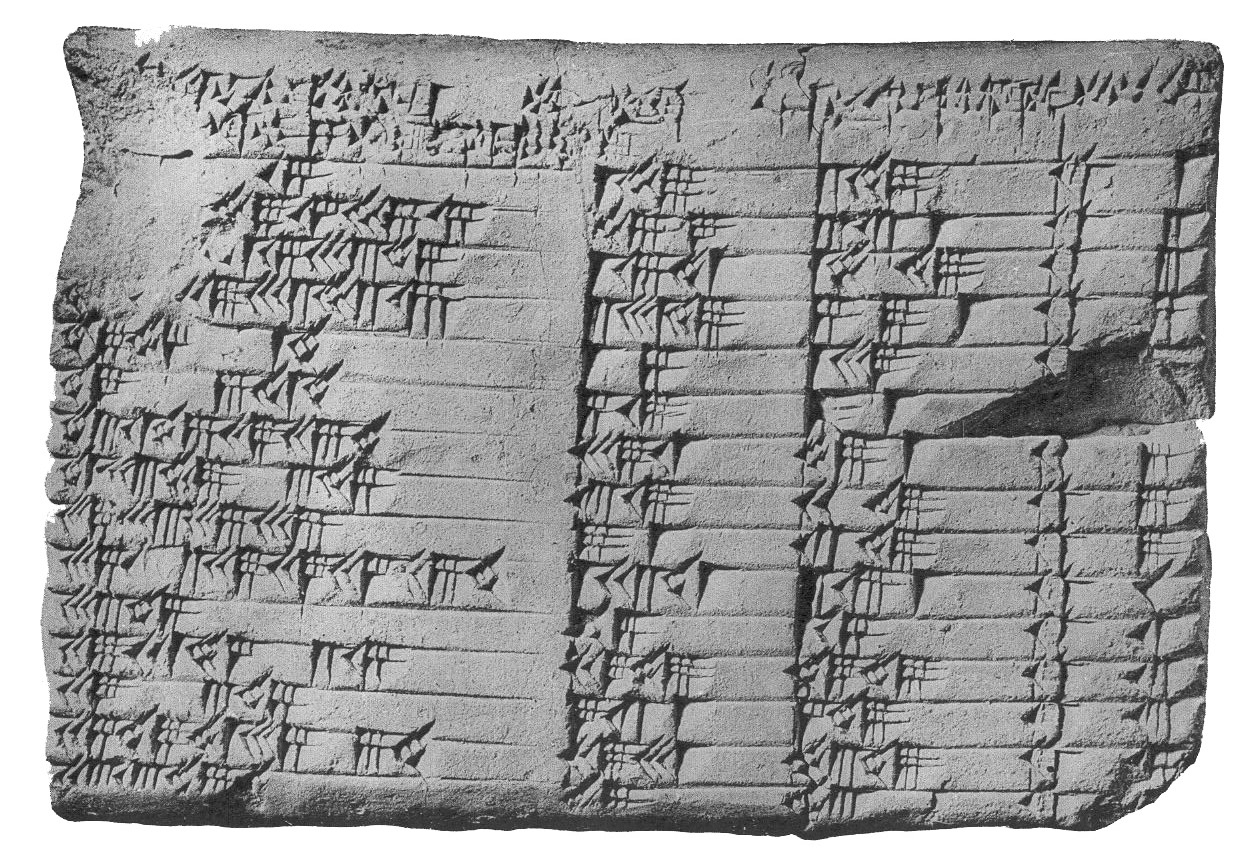
\includegraphics[width=0.68\textwidth,alt={Photograph of the Plimpton 322 clay tablet}]{figures/Plimpton_322.jpg}
  \caption[The Babylonian tablet Plimpton 322]{The Babylonian tablet Plimpton 322, listing Pythagorean triples.}
  \label{fig:plimpton322}
\end{figure}
The triangle with side lengths $3$ and $4$ and a hypotenuse of length $5$ is sometimes called the \define{Egyptian triangle}, since it is believed that the ancient Egyptians used this triangle for practical applications. Some further Pythagorean triples include
\begin{equation*}
  (5,12,13),\qquad (21,20,29),\qquad\text{and}\qquad (15,8,17).
\end{equation*}
The oldest surviving table of Pythagorean triples was created by the Babylonians, in what is now known as the tablet \emph{Plimpton 322}. This clay tablet, which is estimated to date from 1800 BCE, contains a mathematical table written in cuneiform script, where each row describes a Pythagorean triple in sexagesimal notation; that is, in base 60.

Fibonacci devised in his book \emph{Liber Quadratorum (The Book of Squares)} \cite{fibonacci1987} a clever way to quickly show that there are infinitely many Pythagorean triples. If an odd square $a^2$ is the $n$\supth{} odd number, so that $a^2=2n+1$, then by \zcref{exercise:sum-of-odd-numbers} there are positive integers $b$ and $c$ such that
\begin{equation*}
  b^2 = \sum_{i=0}^{n-1}(2i+1),\qquad\text{and}\qquad c^2=\sum_{i=0}^{n}(2i+1)
\end{equation*}
For this choice of $a$, $b$, and $c$, we have
\begin{equation*}
  a^2 + b^2 = c^2.
\end{equation*}

\begin{proposition}
  There are infinitely many Pythagorean triples $(a,b,c)$ such that $c=b+1$.
\end{proposition}

Note that while Fibonacci used the sum of odd numbers to find a triple $(a,b,c)$ of integers such that $a^2+b^2=c^2$, these Fibonacci triples follow the pattern
\begin{equation*}
  (2b + 1) + b^2 = (b+1)^2.
\end{equation*}
Here we immediately see that if $2b+1$ is a square number $a^2$, and indeed any odd square is of this form, then we obtain a Pythagorean triple of the form $(a,b,b+1)$. Rewriting $a=2k+1$, we see that Fibonacci's Pythagorean triples are of the form
\begin{equation*}
  (2k+1,\,2k^2 + 2k,\,2k^2 + 2k+1).
\end{equation*}

The Pythagorean triples $(a,b,c)$ generated by Fibonacci's method always satisfy $c=b+1$. However, we have already seen that $(21,20,29)$ is a Pythagorean triple that is not of this form. Therefore we see that, even though Fibonacci's method can be used to see that there are infinitely many Pythagorean triples, it does not generate all of them.

In the remainder of this section we will derive the classic formula that describes all the Pythagorean triples. The method leading to this formula was described by Euclid in Book X, Proposition 29 and Book 6, Proposition 21 of the Elements.

\begin{definition}
  A \define{primitive Pythagorean triple} is a triple $(a,b,c)$ satisfying
  \begin{equation*}
    a^2 + b^2 = c^2
  \end{equation*}
  such that $\gcd(a,b)=1$.
\end{definition}

\begin{example}
  All the Pythagorean triples generated by Fibonacci's method are primitive, since $\gcd(2b+1,b)=1$.
\end{example}

\begin{lemma}
  For any Pythagorean triple $(a,b,c)$ there is a unique primitive Pythagorean triple $(a',b',c')$ consisting of positive integers for which there is an integer $k$ such that $(ka',kb',kc')=(a,b,c)$.
\end{lemma}

\begin{proof}
  Given a Pythagorean triple $(a,b,c)$, let $k:=\gcd(a,b)$. Since $k\mid a$ and $k\mid b$, it follows from the equation $a^2+b^2=c^2$ that $k\mid c$. Thus, we define
  \begin{equation*}
    a' := a/k, \qquad b' := b/k, \qquad\text{and}\qquad c' := c/k.
  \end{equation*}
  Then $a'$ and $b'$ are relatively prime, and we have
  \begin{equation*}
    a'^2 + b'^2 = \frac{a^2+b^2}{k^2} = \frac{c^2}{k^2} = c'^2.
  \end{equation*}
  The triple $(a',b',c')$ is therefore a primitive Pythagorean triple such that
  \begin{equation*}
    (ka',kb',kc') = (a,b,c).
  \end{equation*}
  For uniqueness, suppose that $(a'',b'',c'')$ is an other such primitive Pythagorean triple, satisfying $(la'',lb'',lc'')=(a,b,c)$. Since $\gcd(a'',b'')=1$, it follows that
  \begin{equation*}
    k=\gcd(a,b)=\gcd(la'',lb'')=l
  \end{equation*}
  Furthermore, since at least one of $a$ or $b$ is nonzero, it follows both $k$ and $l$ are nonzero. Thus we get $a'=a''$ from the equation $ka'=ka''$, and we get $b'=b''$ from the equation $kb'=kb''$. We conclude that $(a',b',c')=(a'',b'',c'')$.
\end{proof}

By the previous lemma we can restrict our attention to primitive Pythagorean triples. Next, we do a parity analysis of the components of a primitive Pythagorean triple to show that exactly one of the components of $(a,b,c)$ in a Pythagorean triple is divisible by $4$. In \zcref{exercise:divisibility-legs-pythagorean-triples} we make the similar claims that exactly one of the components of a Pythagorean triple is divisible by $3$, and exactly one divisible by $5$.

\begin{lemma}\label{lemma:div-4-pythagorean-triple}
  Consider a primitive Pythagorean triple $(a,b,c)$. Then $c$ is odd, exactly one of $a$ and $b$ is divisible by $4$, and the other is odd.
\end{lemma}

\begin{proof}
  Since $(a,b,c)$ is a primitive Pythagorean triple, it is clearly impossible for both $a$ and $b$ to be even. It is also impossible for both of them to be odd, since in that case $c^2$ would be of the form $4k+2$, which is impossible since every square is of the form $4k$ or $4k+1$. Thus, one of $a$ and $b$ is even and the other is odd. This gives us that $c^2$ is odd, which is onlb possible if $c$ is odd.

  It remains to show that the even component among $a$ and $b$ is in fact divisible by $4$. To this end, recall that every square is of the form $8k$, $8k+1$, or $8k+4$. Since $a^2+b^2=c^2$ is of the form $8k+1$, it is impossible for one of the squares $a^2$ or $b^2$ to be of the form $8k+4$. It follows that the even square is of the form $8k$. If $a^2$ is divisible by $8$, then clearly $a$ is divisible by $4$, and likewise if $b^2$ is divisible by $8$ then $b$ is divisible by $4$.
\end{proof}

By the previous lemma we may assume, without loss of generality, that in a primitive Pythagorean triple $(a,b,c)$, the integer $a$ is odd and the integer $b$ is even. Under this assumption, we can show that both $c-a$ and $c+a$ are twice a square, which leads us directly to Euclid's parametrization of the Pythagorean triples.

\begin{lemma}\label{lemma:euclids-parametrization}
  Consider a primitive Pythagorean triple $(a,b,c)$ in which $b$ is even, so that $a$ is odd. Then there are two relatively prime positive integers $s<t$ of opposite parity, such that
  \begin{equation*}
    c-a=2s^2 \qquad\text{and}\qquad c+a=2t^2.
  \end{equation*}
\end{lemma}

\begin{proof}
  By the assumption that $b$ is even, we can write $b=2u$. Then we have
  \begin{equation*}
    (c-a)(c+a) = c^2-a^2 = b^2 = 4u^2.
  \end{equation*}
  Any common divisor $d$ of $c-a$ and $c+a$ must divide their sum $2c$ and their difference $2a$. However, since $a$ and $c$ are relatively prime, it follows that $d\mid 2$. On the other hand, since both $a$ and $c$ are odd it follows that $c\pm a$ is even, which implies that $d=2$. Thus we see that
  \begin{equation*}
    \left(\frac{c-a}{2}\right)\left(\frac{c+a}{2}\right)=u^2
  \end{equation*}
  is a decomposition of a square into relatively prime factors. This implies that each factor is itself a square. More precisely, there are two relatively prime positive integers $s<t$ such that
  \begin{equation*}
    \frac{c-a}{2}=s^2\qquad\text{and}\qquad\frac{c+a}{2}=t^2.
  \end{equation*}
  Furthermore, observe that since $c$ and $a$ are both odd, it follows that one of $c-a$ and $c+a$ is divisible by $4$ and the other is of the form $4k+2$. This implies that one of $s$ and $t$ is even and the other is odd.
\end{proof}

\begin{theorem}[Euclid's Parametrization of the Primitive Pythagorean Triples]\label{theorem:euclids-parametrization}
  For every primitive Pythagorean triple $(a,b,c)$ with $b$ even, we can uniquely determine two relatively prime positive integers $s<t$ of opposite parity such that
  \begin{equation*}
    a=t^2-s^2,\qquad b=2st,\qquad\text{and}\qquad c=t^2+s^2.
  \end{equation*}
\end{theorem}

\begin{proof}
  To prove that two relatively prime integers $0<s<t$ exist as specified, we will use $s$ and $t$ as determined in \zcref{lemma:euclids-parametrization}, where
  \begin{equation*}
    \frac{c-a}{2}=s^2,\qquad\text{and}\qquad\frac{c+a}{2}=t^2.
  \end{equation*}
  A simple calculation shows that $t^2-s^2=a$, and $t^2+s^2=c$. To see that $b=2st$, it suffices to show that $b^2=4s^2t^2$. This follows from the following short calculation:
  \begin{equation*}
    4s^2t^2=(c-a)(c+a)=c^2-a^2=b^2.
  \end{equation*}

  In order to show that $s$ and $t$ are uniquely determined as specified, consider additionally two relatively prime positive integers $u<v$ of opposite parity such that
    \begin{equation*}
    a=v^2-u^2,\qquad b=2uv,\qquad\text{and}\qquad c=v^2+u^2.
  \end{equation*}
  then $c-a=2u^2$ and $c+a=2v^2$, while at the same time we have $c-a=2s^2$ and $c+a=2t^2$. This implies $s^2=u^2$ and $t^2=v^2$. Since all the numbers involved are positive, we obtain that $s=u$ and $t=v$.
\end{proof}

\section{Rational Points on the Unit Circle}

\begin{figure}[t]
  \begin{center}
    \begin{tikzpicture}[scale=3]
      \draw[gray,very thin] (-1.1,-1.1) grid[step=0.2] (1.1,1.1);
      
      \draw[CornflowerBlue,very thick] (0,0) circle (1);
      
      \draw[->] (-1.2,0) -- (1.2,0) node[right] {\(x\)};
      \draw[->] (0,-1.2) -- (0,1.2) node[above] {\(y\)};
      
      \coordinate (P1) at ({377/505},{336/505});
      \draw[thick] (0,0) -- (P1);
      \draw[thick,dashed] (0,0) -- ({377/505},0);
      \draw[thick,dashed] ({377/505},0) -- (P1);
      \draw[thick,fill=white] (P1) circle (.67pt);
    \end{tikzpicture}
  \end{center}
  \caption[The unit circle]{The unit circle consists of all points $(x,y)$ for which the distance to the origin $\sqrt{x^2+y^2}$ is equal to $1$.}
  \label{figure:rational-points-unit-circle}
\end{figure}

The \define{unit circle} consists of all points $(x,y)$ that are a unit distance from the origin. In other words, a point $(x,y)$ in the plane with real number coordinates lies on the unit circle if it satisfies the equation
\begin{equation*}
  x^2+y^2=1.
\end{equation*}
When both coordinates $x$ and $y$ are rational numbers, we say that $(x,y)$ is a \define{rational point} on the unit circle. Primitive Pythagorean triples can be used to obtain such rational points on the unit circle. Every primitive Pythagorean triple $(a,c,b)$ determines the point
\begin{equation*}
  \left(\frac{a}{c},\frac{b}{c}\right),
\end{equation*}
which satisfies $(a/c)^2+(b/c)^2=(a^2+b^2)/c^2= 1$. Thus we see that if $(a,b,c)$ is a primitive Pythagorean triple, then $(a/c,b/c)$ is a rational point on the unit circle. We will show that \emph{every} rational point on the unit circle arises in this way.

\begin{theorem}\label{theorem:correspondence-rational-points-unit-circle}
  There is a bijection between the set of primitive Pythagorean triples $(a,b,c)$, where we allow $a$ and $b$ to be any integer but we maintain the requirement that $c$ is positive, and rational points on the unit circle.
\end{theorem}

\begin{proof}
  We begin by observing that the map
  \begin{equation*}
    (a,b,c)\mapsto \left(\frac{a}{c},\frac{b}{c}\right)
  \end{equation*}
  is an injective function from primitive Pythagorean triples to rational points on the unit circle, since the fractions $a/c$ and $b/c$ are in lowest terms. Therefore, it suffices to show that this map is surjective, meaning that every rational point on the unit circle is of this form.

  We first claim that if $(x,y)$ is a rational point on the unit circle with $x=a/c$ and $y= b/d$ in lowest terms, then we must have $c=d$. This is a special case of \zcref{exercise:equal-denominators-rational-point-on-form}, so the reader who has already solved that exercise may skip ahead.

  The equation $x^2+y^2=1$ can be rearranged to the equation
  \begin{equation*}
    a^2d^2+b^2c^2=c^2d^2.
  \end{equation*}
  It follows that $c^2\mid a^2d^2$ and $d^2\mid b^2c^2$. However, since $\gcd(a,c)=1$ and $\gcd(b,d)=1$, we conclude that $c^2\mid d^2$ and $d^2\mid c^2$, which implies the claim.

  To finish the proof, consider a rational point $(x,y)$ on the unit circle with $x=a/c$ and $y=b/d$. Then we have $c=d$ by the previous claim. It follows that
  \begin{equation*}
    \left(\frac{a\vphantom{b}}{c\vphantom{d}}\right)^2+\left(\frac{b}{c\vphantom{d}}\right)^2=\left(\frac{a\vphantom{b}}{c\vphantom{d}}\right)^2+\left(\frac{b}{d\vphantom{c}}\right)^2=1,
  \end{equation*}
  and we conclude that $(a,b,c)$ is a primitive Pythagorean triple satisfying $(a/c,b/c)=(x,y)$.
\end{proof}

\section[Vieta Jumping]{Vieta Jumping Between Rational Points on the Unit Circle}\label{section:vieta-jumping}

\begin{figure}[t]
  \begin{center}
    \begin{tikzpicture}[scale=4]
      \draw[gray,very thin] (-1.1,-1.1) grid[step=0.2] (1.1,1.1);
      
      \draw[very thick] (0,0) circle (1);
      
      \draw[->] (-1.2,0) -- (1.2,0) node[right] {\(x\)};
      \draw[->] (0,-1.2) -- (0,1.2) node[above] {\(y\)};
      
      \coordinate (P1) at (-1,0);
      \coordinate (P2) at ({5/13},{12/13});
      \coordinate (P3) at ({-2/5},{2/5});
    
      \draw[CornflowerBlue,very thick,->,shorten >=.5ex] (P1) -- (P2);
      
      \draw[fill=black,thick] (P1) circle (.5pt) node[rounded corners=2pt,fill=white,below,inner sep=1pt,yshift=-1ex] {$\textstyle{(-1,0)}$};
      \draw[fill=white,thick] (P2) circle (.5pt) node[rounded corners=2pt,right,fill=white, inner sep=1pt,xshift=.8ex,yshift=2ex] {\(\left(\frac{1-m^2}{1+m^2},\frac{2m}{1+m^2}\right)\)};

      \node[rounded corners=2pt,right,fill=white, inner sep=1pt,xshift=1ex,yshift=-2ex] at (P3) {$\textstyle{y=m(x+1)}$};
    \end{tikzpicture}
  \end{center}
  \caption[Stereographic projection]{A point $(x,y)$ on the unit circle is rational if and only if the line through $(-1,0)$ and $(x,y)$ has a rational slope.}
  \label{figure:stereographic-projection}
\end{figure}

The unit circle is a $1$-dimensional curve through the plane. This suggests that there should be a way of parametrizing all the (rational) points on the unit circle using one rational number as a parameter. We will use a parametrization called the \define{stereographic projection} (see \zcref{figure:rational-points-unit-circle}). The idea of the stereographic projection is to take one particularly simple rational point on the unit circle as our base point---we take the point $(-1,0)$ as our base point---and characterize all the other rational points $(x,y)$ by the slope of the line through the base point $(-1,0)$ and $(x,y)$. Surely, if $(x,y)$ is a rational point on the circle, then the line through $(-1,0)$ and $(x,y)$ will have a rational slope. The question that thus arises is: Does every line through $(-1,0)$ with a rational slope intersect the unit circle in a rational point?

At first consideration, it might not be so clear that this should indeed be the case. The key insights are obtained through Vieta's formulas for the roots of a (quadratic) polynomial, named after the 16\supth{} century French mathematician Fran\c{c}ois Vi\`{e}te. He was one of the first to use letters as parameters in his study of algebraic equations. Vieta's formulas are the essential ingredient in a problem-solving technique called \define{Vieta jumping}.

\begin{theorem}[Vieta's Formulas for the Roots of a Quadratic Polynomial]\label{theorem:vieta-formulas-quadratic}
  Consider a polynomial of the form $t^2-Bt+C$ and suppose that $r$ is a root of this polynomial. Then the other root $s$ satisfies the relations
  \begin{equation*}
    r+s=B\qquad\text{and}\qquad rs=C.
  \end{equation*}
\end{theorem}

\begin{proof}
  The two roots of a quadratic polynomial $f(t)=t^2-Bt+C$ are $r$ and $s$ if and only if we can write $f(t)$ in the form
  \begin{equation*}
    f(t)=(t-r)(t-s).
  \end{equation*}
  However, if this equation holds, then we find that
  \begin{equation*}
    t^2-(r+s)t+rs=t^2-Bt+C.
  \end{equation*}
  The asserted relations now follow by comparing coefficients.
\end{proof}

A corollary of the previous theorem is that if $B$ and $C$ are rational numbers and $r$ is a rational root of the polynomial $t^2-Bt+C$, then the other root $s$ is also rational.

\begin{theorem}\label{theorem:stereographic-projection-unit-circle}
  Consider the line given by the equation $y=m(x+1)$, which has slope $m$ and passes through the point $(-1,0)$. This line intersects the unit circle at the point
  \begin{equation*}
    \left(\frac{1-m^2}{1+m^2},\frac{2m}{1+m^2}\right).
  \end{equation*}
  Consequently, the line $y=m(x+1)$ intersects the unit circle at a rational point other than $(-1,0)$ if and only if the slope $m$ is rational.
\end{theorem}

\begin{proof}
  In order to find the two points $(x,y)$ on the intersection of the line $y=m(x+1)$ and the unit circle, we must solve the equation
  \begin{equation*}
    x^2+m^2(x+1)^2=1.
  \end{equation*}
  By rearranging, we find that it is equivalent to solve the equation
  \begin{equation*}
    x^2 + \frac{2m^2}{1+m^2}x + \frac{m^2-1}{1+m^2} = 0.
  \end{equation*}
  Since we already know that there is one root at $-1$, we can find the other root by Vieta's formulas given in \zcref{theorem:vieta-formulas-quadratic}: The other intersection point is at $(x,y)$, where
  \begin{equation*}
    x=\frac{1-m^2}{1+m^2}\qquad\text{and}\qquad y=\frac{2m}{1+m^2}.
  \end{equation*}

  For the final claim, it is clear that if $m \in \mathbb{Q}$, then both $x$ and $y$ are rational numbers. Conversely, if $(x,y)$ is a rational point on the unit circle distinct from $(-1,0)$, then we have $-1<x\leq 1$ and $m = \tfrac{y}{x+1}$, which is a quotient of rational numbers and thus rational.
\end{proof}

\begin{remark}
  If $(a,b,c)$ is a primitive Pythagorean triple, then the corresponding rational point on the unit circle is $(a/c,b/c)$,
  and the slope of the line through $(-1,0)$ and this point is
  \begin{equation*}
    \frac{b}{a+c}.
  \end{equation*}
\end{remark}

\section{The Tree of Primitive Pythagorean Triples}\label{section:tree-of-pythagorean-triples}

In 1934, the Swedish senior high school teacher B.~Berggren discovered that the primitive Pythagorean triples can naturally be given the structure of a ternary tree \cite{berggren1934}. More precisely, he discovered that all primitive Pythagorean triples can be obtained by iterated application of three linear operations, starting with the triple $(3,4,5)$. The three linear operations found by Berggren are the three matrices
\begin{equation*}
  A =
  \left(
    \begin{matrix}
      1 & -2 & 2 \\
      2 & -1 & 2 \\
      2 & -2 & 3
    \end{matrix}
  \right),\qquad
  B =
  \left(
    \begin{matrix}
      1 & 2 & 2 \\
      2 & 1 & 2 \\
      2 & 2 & 3
    \end{matrix}
  \right),\qquad\text{and}\qquad
  C =
  \left(
    \begin{matrix}
      -1 & 2 & 2 \\
      -2 & 1 & 2 \\
      -2 & 2 & 3
    \end{matrix}
  \right).
\end{equation*}

To rediscover Berggren's matrices and his ternary tree, we will use the technique of Vieta jumping, which we have already used in the previous section to establish a correspondence between primitive Pythagorean triples and rational points on the unit circle. We begin with a generalization of \zcref{theorem:stereographic-projection-unit-circle}, where we established the stereographic projection of the (rational) points on the unit circle.

\begin{theorem}[Vieta Jumping for Rational Points on the Unit Circle]\label{theorem:vieta-jumping-rational-points-unit-circle}
  Consider a rational point $(x,y)$ on the unit circle. For any point $(u,v)$ with rational coordinates such that $u\neq x$, consider the line through $(u,v)$ and $(x,y)$, whose slope is
  \begin{equation*}
    m:=\frac{y-v}{x-u}.
  \end{equation*}
  This line intersects the unit circle in a second rational point $(x',y')$. Moreover, $x$ and $x'$ satisfy the relation
  \begin{equation*}
    xx' = \frac{(mu-v)^2 -1}{1+m^2}.
  \end{equation*}
\end{theorem}

\begin{proof}
  First, we parametrize the line through $(u,v)$ and $(x,y)$ as a function of $t$ given by
  \begin{equation*}
    s(t) := m(t-u)+v,
  \end{equation*}
  where the slope $m$ is defined by $m:=\tfrac{y-v}{x-u}$. In order to find the intersection points of this line with the unit circle, we have to solve the equation $t^2+s(t)^2=1$. We can simplify this equation as follows:
  \begin{align*}
    0 & = t^2 + (v+m(t-u))^2 - 1 \\
      & = t^2 + v^2 + 2vm(t-u) +m^2(t^2-2ut + u^2) -1 \\
      & = (1+m^2)t^2 + (2vm - 2um^2)t + (mu-v)^2 -1.
  \end{align*}
  Dividing through by $1+m^2$, we see that $x$ and $x'$ are the roots of the quadratic equation
  \begin{equation*}
    t^2 + \frac{2vm - 2um^2}{1+m^2}t + \frac{(mu-v)^2 -1}{1+m^2}=0.
  \end{equation*}
  We have thus reached a quadratic equation of the form $t^2+Bt+C$, which has by assumption one rational solution at $t=x$. It follows from \zcref{theorem:vieta-formulas-quadratic} that the second solution $x'$ satisfies the Vieta relation
  \begin{equation*}
    xx' = \frac{(mu-v)^2 -1}{1+m^2}.\qedhere
  \end{equation*}
\end{proof}

\begin{figure}[tbp]
  \begin{center}
    \begin{tikzpicture}[scale=4]
      \draw[gray,very thin] (-1.1,-1.1) grid[step=0.2] (1.1,1.1);
      
      \draw[thick,Gray] (-1,-1) rectangle (1,1);
      
      \draw[very thick] (0,0) circle (1);
      
      \draw[->] (-1.2,0) -- (1.2,0) node[right] {\(x\)};
      \draw[->] (0,-1.2) -- (0,1.2) node[above] {\(y\)};
      
      \coordinate (P1) at ({117/125},{44/125});
      \coordinate (P2) at ({45/53},{-28/53});
      \coordinate (P3) at ({5/13},{12/13});
      \coordinate (P4) at ({-3/5},{4/5});
    
      \draw[DarkOrchid,very thick,dashed] (1,1) -- (P1);
      \draw[DarkOrchid,very thick,->,shorten >=2ex] (P1) -- (P2);
      \draw[Green,very thick,dashed] (1,-1) -- (P2);
      \draw[Green,very thick,->,shorten >=0.8ex] (P2) -- (P3);
      \draw[YellowOrange,very thick,dashed] (1,1) -- (P3);
      \draw[YellowOrange,very thick,->,shorten >=1.5ex] (P3) -- (P4);
      \draw[CornflowerBlue,very thick,dashed] (-1,1) -- (P4);
      \draw[CornflowerBlue,very thick,->,shorten >=0.8ex] (P4) -- (1,0);
      
      \draw[fill=white,thick] (P1) circle (.5pt) node[rounded corners=2pt,right,fill=white, inner sep=1pt,xshift=1ex] {\(\left(\frac{117}{125}, \frac{44}{125}\right)\)};
      \draw[fill=white,thick] (P2) circle (.5pt) node[rounded corners=2pt,right,fill=white, inner sep=1pt,xshift=1.2ex,yshift=-1pt] {\(\left(\frac{45}{53},\frac{-28}{53}\right)\)};
      \draw[fill=white,thick] (P3) circle (.5pt) node[rounded corners=2pt,above,fill=white, inner sep=1pt,yshift=1.4ex] {\(\left(\frac{5}{13},\frac{12}{13}\right)\)}; 
      \draw[fill=white,thick] (P4) circle (.5pt) node[rounded corners=2pt,below,fill=white, inner sep=1pt,yshift=-1.5ex,xshift=-1ex] {\(\left(\frac{-3}{5},\frac{4}{5}\right)\)};
      \draw[fill=black,thick] (1,0) circle (.5pt);
      
    \end{tikzpicture}
  \end{center}
  \caption[Vieta jumps between rational points on the unit circle]{For any rational point $(x,y)$ on the unit circle apart from $(0,\pm1)$ and $(\pm1,0)$, draw a straight line through it from the outer corner of its quadrant to find a new rational point $(x',y')$ on the unit circle. The common denominator of the fractions $x'$ and $y'$, when brought to lowest terms, is strictly smaller than that of $x$ and $y$, so that this process eventually terminates at $(0,\pm1)$ or $(\pm1,0)$.}
  \label{figure:vieta-jumps-pythagorean-triples}
\end{figure}

By making a suitable choice for the rational point $(u,v)$, the previous theorem can be used to find, for each rational point $(x,y)$ on the unit circle corresponding to a primitive Pythagorean triple $(a,b,c)$ with $0<c$, which we assume to be nontrivial in the sense that $ab\neq 0$, a new rational point $(x',y')$ on the unit circle corresponding to a primitive Pythagorean triple $(a',b',c')$ satisfying $0<c'<c$. That is, we will find a procedure to step from a primitive Pythagorean triple to a new Pythagorean triple with a smaller hypotenuse.

The suitable choice of $(u,v)$ that we just alluded is given by
\begin{equation*}
  u:= \sgn(a)\qquad\text{and}\qquad v:=\sgn(b).
\end{equation*}
In other words, the point $(u,v)$ is the nearest corner of the $2$-by-$2$ square centered at the origin to the rational point $(x,y)$ on the unit circle.
The procedure $(a,b,c)\mapsto (a',b',c')$ of stepping from one Pythagorean triple to a new one with a smaller hypotenuse is illustrated in the following example, which is accompanied by \zcref{figure:vieta-jumps-pythagorean-triples}.

\begin{example}
  Consider the Pythagorean triple $(a,b,c):=(117,44,125)$, which corresponds to the rational point $(x,y):=(117/125,44/125)$ on the unit circle. Since both $a$ and $b$ are positive, we have $u=v=1$, and the new point $(x',y')$ the unit circle and on the line through $(u,v)$ and $(x,y)$ satisfies
  \begin{equation*}
    xx'=\frac{(m-1)^2-1}{1+m^2},
  \end{equation*}
  where $m=\tfrac{y-1}{x-1}$. Since $x=a/c$ and $y=b/c$, we can rearrange the previous Vieta relation to obtain that
  \begin{equation*}
    xx'=\frac{(b-a)^2-(a-c)^2}{(a-c)^2+(b-c)^2}=\frac{73^2-8^2}{8^2+81^2}.
  \end{equation*}
  From these calculations, we obtain that $x'=45/53$ and $y'=-28/53$, which corresponds to the primitive Pythagorean triple $(45,-28,53)$, which indeed has a hypotenuse satisfying $53<125$.
\end{example}

Recall that for each rational point $(x,y)$ on the unit circle, we can write $x=a/c$ and $y=b/c$ in lowest terms with identical denominators, which we always take to be positive. This observation is a direct consequence of \zcref{theorem:correspondence-rational-points-unit-circle}. Thus, we can unambiguously refer to the \emph{common denominator} of any rational point on the unit circle. We also recall that for any two positive integers $a$ and $b$, we have
\begin{equation*}\label{equation:instance-am-gm}
  2ab\leq a^2+b^2. \tag{\textasteriskcentered}
\end{equation*}
This inequality, which is an instance of the AM--GM inequality, follows from the observation that $(a-b)^2=a^2-2ab+b^2\geq 0$.

\begin{theorem}[Pythagorean Descent]\label{theorem:pythagorean-descent}
  Consider a primitive Pythagorean triple $(a,b,c)$ with $c>1$, corresponding to the rational point $(x,y)$ on the unit circle given by
  \begin{equation*}
    x=\frac{a}{c}\qquad\text{and}\qquad y=\frac{b}{c}.
  \end{equation*}
  Furthermore, consider one of the corner points $(u,v)=(\pm 1,\pm 1)$ of the $2$-by-$2$ square centered at the origin. Then the second intersection point $(x',y')$ of the line through $(u,v)$ and $(x,y)$ and the unit circle, as determined by \zcref{theorem:vieta-jumping-rational-points-unit-circle}, corresponds to the primitive Pythagorean triple $(a',b',c')$ given by
  \begin{equation*}
    \begin{pmatrix}
      a' \\
      b' \\
      c'
    \end{pmatrix}
    =
    \begin{pmatrix}
      -1 & -2uv & 2u \\
      -2uv & -1 & 2v \\
      -2u & -2v & 3
    \end{pmatrix}
    \begin{pmatrix}
      a \\
      b \\
      c
    \end{pmatrix}
  \end{equation*}
  Moreover, when $u =\sgn(x)$ and $v =\sgn(y)$, then we have $0<c'<c$.
\end{theorem}

\begin{proof}
  The rational point $(x',y')$ obtained from \zcref{theorem:vieta-jumping-rational-points-unit-circle} satisfies the relation
  \begin{equation*}
    xx' = \frac{(mu-v)^2 -1}{1+m^2},
  \end{equation*}
  where $m:=\tfrac{y-v}{x-u}$ is the slope of the line through $(u,v)$ and $(x,y)$. Given that $x=a/c$ and $y=b/c$, we see that
  \begin{equation*}
    m=\frac{b-vc}{a-uc}.
  \end{equation*}
  We use this to rewrite Vieta's relation between $x$ and $x'$ as follows:
  \begin{equation*}
    xx' = \frac{(bu-av)^2-(a-uc)^2}{(a-uc)^2+(b-vc)^2}.
  \end{equation*}
  Given that $u^2=v^2=1$ and $a^2+b^2=c^2$, we compute this quantity as follows:
  \begin{equation*}
    xx'= \frac{(bu-av)^2-(a-uc)^2}{(a-uc)^2+(b-vc)^2} = \frac{b^2-c^2-2uvab+2uac}{-2uac-2vbc + a^2+b^2+2c^2}=\frac{a}{c}\frac{-a-2uvb+2uc}{-2ua-2vb + 3c}.
  \end{equation*}
  Thus, we obtain the following expressions for $a'$ and $c'$, so that $x'=a'/c'$:
  \begin{align*}
    a' & = -a-2uvb+2uc, \\
    c' & = -2ua-2vb + 3c.
  \end{align*}
  Now we can verify that $b'=-2uva-b+2vc$ by checking that, taking this as our definition for $b'$, we have $a'^2+b'^2=c'^2$ and
  \begin{equation*}
    \frac{b'-b}{a'-a}=m.
  \end{equation*}
  Both of these identities are verified by a quick calculation, which we leave to the reader. It follows that, given a primitive Pythagorean triple $(a,b,c)$, the Pythagorean triple $(a',b',c')$ is determined by the matrix multiplication
  \begin{equation*}
    \begin{pmatrix}
      a' \\
      b' \\
      c'
    \end{pmatrix}
    =
    \begin{pmatrix}
      -1 & -2uv & 2u \\
      -2uv & -1 & 2v \\
      -2u & -2v & 3
    \end{pmatrix}
    \begin{pmatrix}
      a \\
      b \\
      c
    \end{pmatrix}
  \end{equation*}
  
  If $M$ is the matrix in the above equation, it is immediate from the construction of $M$ that $M^2=I$, the identity matrix. Indeed, jumping from $(x,y)$ to $(x',y')$ using the point $(u,v)$, and jumping again from $(x',y')$ using the same point $(u,v)$ reverses the process and lands us back at $(x,y)$. This implies that any common divisors of $(a',b',c')$ are also common divisors of $(a,b,c)$. Since $(a,b,c)$ is primitive, it follows that $(a',b',c')$ is also primitive.
  
  The final claim is that $c':= 3c-2\abs{a}-2\abs{b}$ satisfies $0<c'<c$. By rearranging the terms, we see that these strict inequalities are equivalent to the strict inequalities
  \begin{equation*}
    2c<2\abs{a}+2\abs{b}<3c.
  \end{equation*}
  We can prove these strict inequalities by proving that they hold for the squares:
  \begin{equation*}
    4c^2<4(\abs{a}+\abs{b})^2<9c^2.
  \end{equation*}
  To see this, we note that $(\abs{a}+\abs{b})^2=a^2+2\abs{a}\abs{b} + b^2= c^2+2\abs{a}\abs{b}$. This immediately implies that $c^2\leq (\abs{a}+\abs{b})^2$. Furthermore, we have the inequality $2\abs{a}\abs{b}\leq a^2+b^2=c^2$ by the inequality stated in \zcref{equation:instance-am-gm}. Thus we obtain that
  \begin{equation*}
    4c^2< 4(\abs{a}+\abs{b})^2 = 4c^2+8\abs{a}\abs{b} \leq 4c^2 + 4c^2<9c^2.\qedhere
  \end{equation*}
\end{proof}

\begin{figure}[tbp]
  \centering
  \begingroup

  \tikzset{
    treenode/.style={circle,draw,thick,inner sep=1.5pt},
    tree/.style={
      grow=up,
      level distance=10mm,
      edge from parent/.style={draw,thick,<-,shorten <= 2pt, shorten >= 2pt},
      every node/.style={treenode}
    }
  }
  
  \newcommand{\DrawRootedTree}[2][]{%
    \begin{scope}[tree,#1]%
      \node {} #2;%
    \end{scope}%
  }

  \begin{tikzpicture}
    
    \DrawRootedTree[xshift=-4cm]{%
      child { node {}
        child { node {} }
        child { node {} }
      }
      child { node {} }
    }
    
    \DrawRootedTree{%
      child { node {}
        child { node {} }
        child { node {}
          child { node {} }
        }
      }
    }
    
    \DrawRootedTree[xshift=4cm]{%
      child { node {}
        child { node {} }
      }
      child[missing]
      child { node {}
        child { node {} }
        child { node {} }
      }
    }
    
  \end{tikzpicture}

  \endgroup
  \caption[A forest]{A forest.}
  \label{figure:forest}
\end{figure}

\zcrefnamed{theorem:pythagorean-descent} can be used to determine a ternary tree structure on the set of primitive Pythagorean triples. We will define trees to be forests consisting of a single tree. Mathematically, a \define{forest} is defined as a set $F$ equipped with a \define{height function} $h:F\to \mathbb{N}$, and for each height $n$ a \define{parent function}
\begin{equation*}
  p : \{x\in F\mid h(x)=n+1\}\to \{x\in F\mid h(x)=n\}.
\end{equation*}
Given a forest $F$, an element $x\in F$ is called a \define{node}; a node $x$ of height $0$ is called a \define{root}; the node $p(x)$ is called the \define{parent} of $x$; and for any node $y$, all the nodes $x$ whose parent is $y$ are called the \define{children} of $y$. A forest is said to be a \define{tree} if it contains exactly one root. We note that a forest can contain nodes of arbitrary height; that is, mathematical trees can be infinitely tall. In \zcref{figure:forest} we have drawn an example of a forest.


\begin{figure}[tbp]
  \begin{center}
    \begin{tikzpicture}[scale=4]
      \draw[gray,very thin] (-1.1,-1.1) grid[step=0.2] (1.1,1.1);
      
      \draw[thick,Gray] (-1,-1) rectangle (1,1);
      
      \draw[very thick] (0,0) circle (1);
      
      \draw[->] (-1.2,0) -- (1.2,0) node[right] {\(x\)};
      \draw[->] (0,-1.2) -- (0,1.2) node[above] {\(y\)};
      
      \coordinate (P1) at ({117/125},{44/125});
      \coordinate (P2) at ({45/53},{-28/53});
      \coordinate (P3) at ({5/13},{12/13});
      \coordinate (P4) at ({-3/5},{4/5});

      \coordinate (P12) at ({-207/305},{224/305});
      \coordinate (P13) at ({-95/193},{-168/193});
    
      \draw[DarkOrchid,very thick,dashed] (1,1) -- (P1);
      \draw[DarkOrchid,very thick,->,shorten >=2ex] (P1) -- (P2);
      \draw[Green,very thick,dashed] (1,-1) -- (P2);
      \draw[Green,very thick,->,shorten >=0.8ex] (P2) -- (P3);
      \draw[YellowOrange,very thick,dashed] (1,1) -- (P3);
      \draw[YellowOrange,very thick,->,shorten >=1.5ex] (P3) -- (P4);
      \draw[CornflowerBlue,very thick,dashed] (-1,1) -- (P4);
      \draw[CornflowerBlue,very thick,->,shorten >=0.8ex] (P4) -- (1,0);
      \draw[DarkOrchid,very thick,dashed] (-1,1) -- (P12);
      \draw[DarkOrchid,very thick,dashed] (-1,-1) -- (P13);
      \draw[DarkOrchid,very thick,->,shorten >=2ex] (P12) -- (P2);
      \draw[DarkOrchid,very thick,->,shorten >=2ex] (P13) -- (P2);
      
      \draw[fill=white,thick] (P1) circle (.5pt) node[rounded corners=2pt,right,fill=white, inner sep=1pt,xshift=1ex] {\(\left(\frac{117}{125}, \frac{44}{125}\right)\)};
      \draw[fill=white,thick] (P2) circle (.5pt) node[rounded corners=2pt,right,fill=white, inner sep=1pt,xshift=1.2ex,yshift=-1pt] {\(\left(\frac{45}{53},\frac{-28}{53}\right)\)};
      \draw[fill=white,thick] (P3) circle (.5pt); 
      \draw[fill=white,thick] (P4) circle (.5pt);
      \draw[fill=black,thick] (1,0) circle (.5pt);
      \draw[fill=white,thick] (P12) circle (.5pt) node[rounded corners=2pt,left,fill=white, inner sep=1pt,xshift=-1ex,yshift=-3ex] {\(\left(\frac{-207}{305}, \frac{224}{305}\right)\)};
      \draw[fill=white,thick] (P13) circle (.5pt) node[rounded corners=2pt,above,fill=white, inner sep=1pt,yshift=2ex] {\(\left(\frac{-95}{193}, \frac{-168}{193}\right)\)};
    \end{tikzpicture}
  \end{center}
  \caption[The forest of rational points on the unit circle]{Each rational point on the unit circle other than $(\pm 1,0)$ or $(0,\pm 1)$ is the target of a Vieta jump from three rational points on the unit circle with larger common denominator, one for each quadrant other than its own. Here, the purple, green, and orange jumps are drawn exactly as in \zcref{figure:vieta-jumps-pythagorean-triples}. The point $(45/53,-28/53)$ is the target of three jumps, each drawn in blue. Since each rational point is the target of three Vieta jumps that decrease the common denominator, we see that the rational points on the unit circle can be organized in a forest consisting of four trees, where the four nodes at height $0$ are the points $(\pm 1,0)$ and $(0,\pm 1)$.}
  \label{figure:forest-rational-points-unit-circle}
\end{figure}

\begin{example}[The forest of rational points on the unit circle]
  In \zcrefnamed{theorem:pythagorean-descent}, we showed that for each rational point on the unit circle other than $(\pm 1,0)$ or $(0,\pm 1)$, we can jump to another rational point whose positive common denominator is strictly smaller than that of the original point. If the new point is not one of the points $(\pm 1,0)$ or $(0,\pm 1)$, we can jump again to yet another rational point whose common denominator is still smaller. Starting at $(x_0,y_0):=(x,y)$, repeating this process results in a sequence of rational points $(x_n,y_n)$ on the unit circle, whose common denominators strictly decrease as the sequence progresses. Since a sequence of positive integers cannot be infinitely long, we see that this sequence must terminate. That is, in a finite number of jumps we must reach one of the points $(\pm 1,0)$ or $(0,\pm 1)$.

  For any rational point $(x,y)$ on the unit circle, let $h(x,y)$ be the least number of jumps required to reach one of the points $(\pm 1,0)$ or $(0,\pm 1)$. Furthermore, if $(x,y)$ is of height $n+1$, so that it is neither $(\pm 1,0)$ nor $(0,\pm 1)$, let $p(x,y):=(x',y')$ be the target of the jump from $(x,y)$. This height and parent function gives the set of rational points on the unit circle the structure of a forest with four roots, the points $(\pm 1,0)$ and $(0,\pm 1)$. In \zcref{figure:forest-rational-points-unit-circle} we displayed one branching point in this forest, along with the path to its root.

  We observe that in this forest, each root $(\pm 1,0)$ or $(0,\pm 1)$ has two children. These are the eight points $(\pm 3/5,\pm 4/5)$ and $(\pm 4/5,\pm 3/5)$. Any rational point on the unit circle other than a root has exactly three children, one in each quadrant other than its own.

  We also observe that the forest of rational points on the unit circle possesses some important symmetries. Each rotation by $90^\circ$ and each reflection along the axis of abscissas, the line $y=x$, the axis of ordinates, and the line $y=-x$ maps rational points on the unit circle to rational points on the unit circle in such a way that the height and parent functions are preserved. To see this, observe that each of those symmetries reflects a point $(x,y)$ on the unit circle to one of the points $(\pm x,\pm y)$ or $(\pm y,\pm x)$.
\end{example}

\begin{example}[The tree of primitive Pythagorean triples]
  We will now use the forest of rational points on the unit circle to construct the tree of primitive Pythagorean triples, and derive Berggren's matrices.

  The matrix we used in \zcrefnamed{theorem:pythagorean-descent} to jump from a primitive Pythagorean triple $(a,b,c)$ with $1<c$ to a new primitive Pythagorean triple $(a',b',c')$ was defined as
\begin{equation*}
  M_{u,v}
  :=
  \begin{pmatrix}
    -1 & -2uv & 2u \\
    -2uv & -1 & 2v \\
    -2u & -2v & 3
  \end{pmatrix}
  .
\end{equation*}
When $u:=\sgn(a)$ and $v:=\sgn(b)$, then the new Pythagorean triple satisfies $0<c'<c$. This implies that for any of the three other choices of $(u,v)$, the new Pythagorean triple satisfies $c<c'$.

From now on, we will assume that $(a,b,c)$ is a primitive Pythagorean triple in which all of $a$, $b$, and $c$ are positive integers, and furthermore $b$ is even. To step upwards along the tree, we set $u=\pm 1$ and $v=\pm 1$ so that at least one of $u$ and $v$ is $-1$. This results in a new Pythagorean triple corresponding to a rational point on the unit circle in the quadrant of the point $(u,v)$. To reflect this rational point back to the quadrant with positive $x$- and $y$-cordinates, we compose the matrix $M_{u,v}$ with one further linear operation as follows:
\begin{equation*}
  \begin{pmatrix}
    u & 0 & 0 \\
    0 & v & 0 \\
    0 & 0 & 1
  \end{pmatrix}
  \begin{pmatrix}
    -1 & -2uv & 2u \\
    -2uv & -1 & 2v \\
    -2u & -2v & 3
  \end{pmatrix}
  =
  \begin{pmatrix}
    -u & -2v & 2 \\
    -2u & -v & 2 \\
    -2u & -2v & 3
  \end{pmatrix}
\end{equation*}
Instantiating these matrices at $(u,v)=(-1,1)$, $(1,-1)$, and $(-1,-1)$ gives the matrices that Berggren discovered in 1934:
\begin{equation*}
  A =
  \left(
    \begin{matrix}
      1 & -2 & 2 \\
      2 & -1 & 2 \\
      2 & -2 & 3
    \end{matrix}
  \right),\qquad
  B =
  \left(
    \begin{matrix}
      1 & 2 & 2 \\
      2 & 1 & 2 \\
      2 & 2 & 3
    \end{matrix}
  \right),\qquad\text{and}\qquad
  C =
  \left(
    \begin{matrix}
      -1 & 2 & 2 \\
      -2 & 1 & 2 \\
      -2 & 2 & 3
    \end{matrix}
  \right)
\end{equation*}
By \zcrefnamed{theorem:pythagorean-descent} it follows that all primitive Pythagorean triples can be obtained by iteratively applying the matrices $A$, $B$, and $C$ given above. This tree is displayed in \zcref{figure:tree-of-pythagorean-triples}.
\end{example}

% \clearpage

\begin{figure}[p]
  \centering
  \begin{tikzpicture}[
   font=\small,
    grow'=right,
    level 1/.style={sibling distance=15em,level distance=8em},
    level 2/.style={sibling distance=5em,level distance=8em},
    level 3/.style={sibling distance=1.67em,level distance=10em},
    edge from parent/.style={draw,black}
    ]
    \node {$(3,4,5)$}
    child[edge from parent/.style={draw,YellowOrange,very thick}] {
      node {$(5,12,13)$}
      child[edge from parent/.style={draw,thin,black}] {
        node {$(7,24,25)$}
        child[edge from parent/.style={draw,thin,black}] {node {$(9,40,41)$}}
        child[edge from parent/.style={draw,thin,black}] {node {$(105,88,137)$}}
        child[edge from parent/.style={draw,thin,black}] {node {$(91,60,109)$}}
      }
      child[edge from parent/.style={draw,thin,black}] {
        node {$(55,48,73)$}
        child[edge from parent/.style={draw,thin,black}] {node {$(105,208,233)$}}
        child[edge from parent/.style={draw,thin,black}] {node {$(297,304,425)$}}
        child[edge from parent/.style={draw,thin,black}] {node {$(187,84,205)$}}
      }
      child[edge from parent/.style={draw,Green,very thick}] {
        node {$(45,28,53)$}
        child[edge from parent/.style={draw,DarkOrchid,very thick}] {node {$(95,168,193)$}}
        child[edge from parent/.style={draw,DarkOrchid,very thick}] {node {$(207,224,305)$}}
        child[edge from parent/.style={draw,DarkOrchid,very thick}] {node {$(117,44,125)$}}
      }
    }
    child {
      node {$(21,20,29)$}
      child {
        node {$(39,80,89)$}
        child {node {$(57,176,185)$}}
        child {node {$(377,336,505)$}}
        child {node {$(299,180,349)$}}
      }
      child {
        node {$(119,120,169)$}
        child {node {$(217,456,505)$}}
        child {node {$(697,696,985)$}}
        child {node {$(459,220,509)$}}
      }
      child {
        node {$(77,36,85)$}
        child {node {$(175,288,337)$}}
        child {node {$(319,360,481)$}}
        child {node {$(165,52,173)$}}
      }
    }
    child {
      node {$(15,8,17)$}
      child {
        node {$(33,56,65)$}
        child {node {$(51,140,149)$}}
        child {node {$(275,252,373)$}}
        child {node {$(209,120,241)$}}
      }
      child {
        node {$(65,72,97)$}
        child {node {$(115,252,277)$}}
        child {node {$(403,396,565)$}}
        child {node {$(273,136,305)$}}
      }
      child {
        node {$(35,12,37)$}
        child {node {$(85,132,157)$}}
        child {node {$(133,156,205)$}}
        child {node {$(63,16,65)$}}
      }
    };
  \end{tikzpicture}
  \caption[The tree of primitive Pythagorean triples]{The tree of primitive Pythagorean triples. The edges that were drawn in orange, green, or purple in \zcref{figure:forest-rational-points-unit-circle} have been drawn here in the same color.}
  \label{figure:tree-of-pythagorean-triples}
\end{figure}

% \clearpage

\section{Squares in Arithmetic Progressions}\label{sec:squares-in-aps}

\begin{figure}[t]
  \centering
  \begin{tikzpicture}
    \node[inner sep=0pt, rounded corners=0.2em, clip] {%
      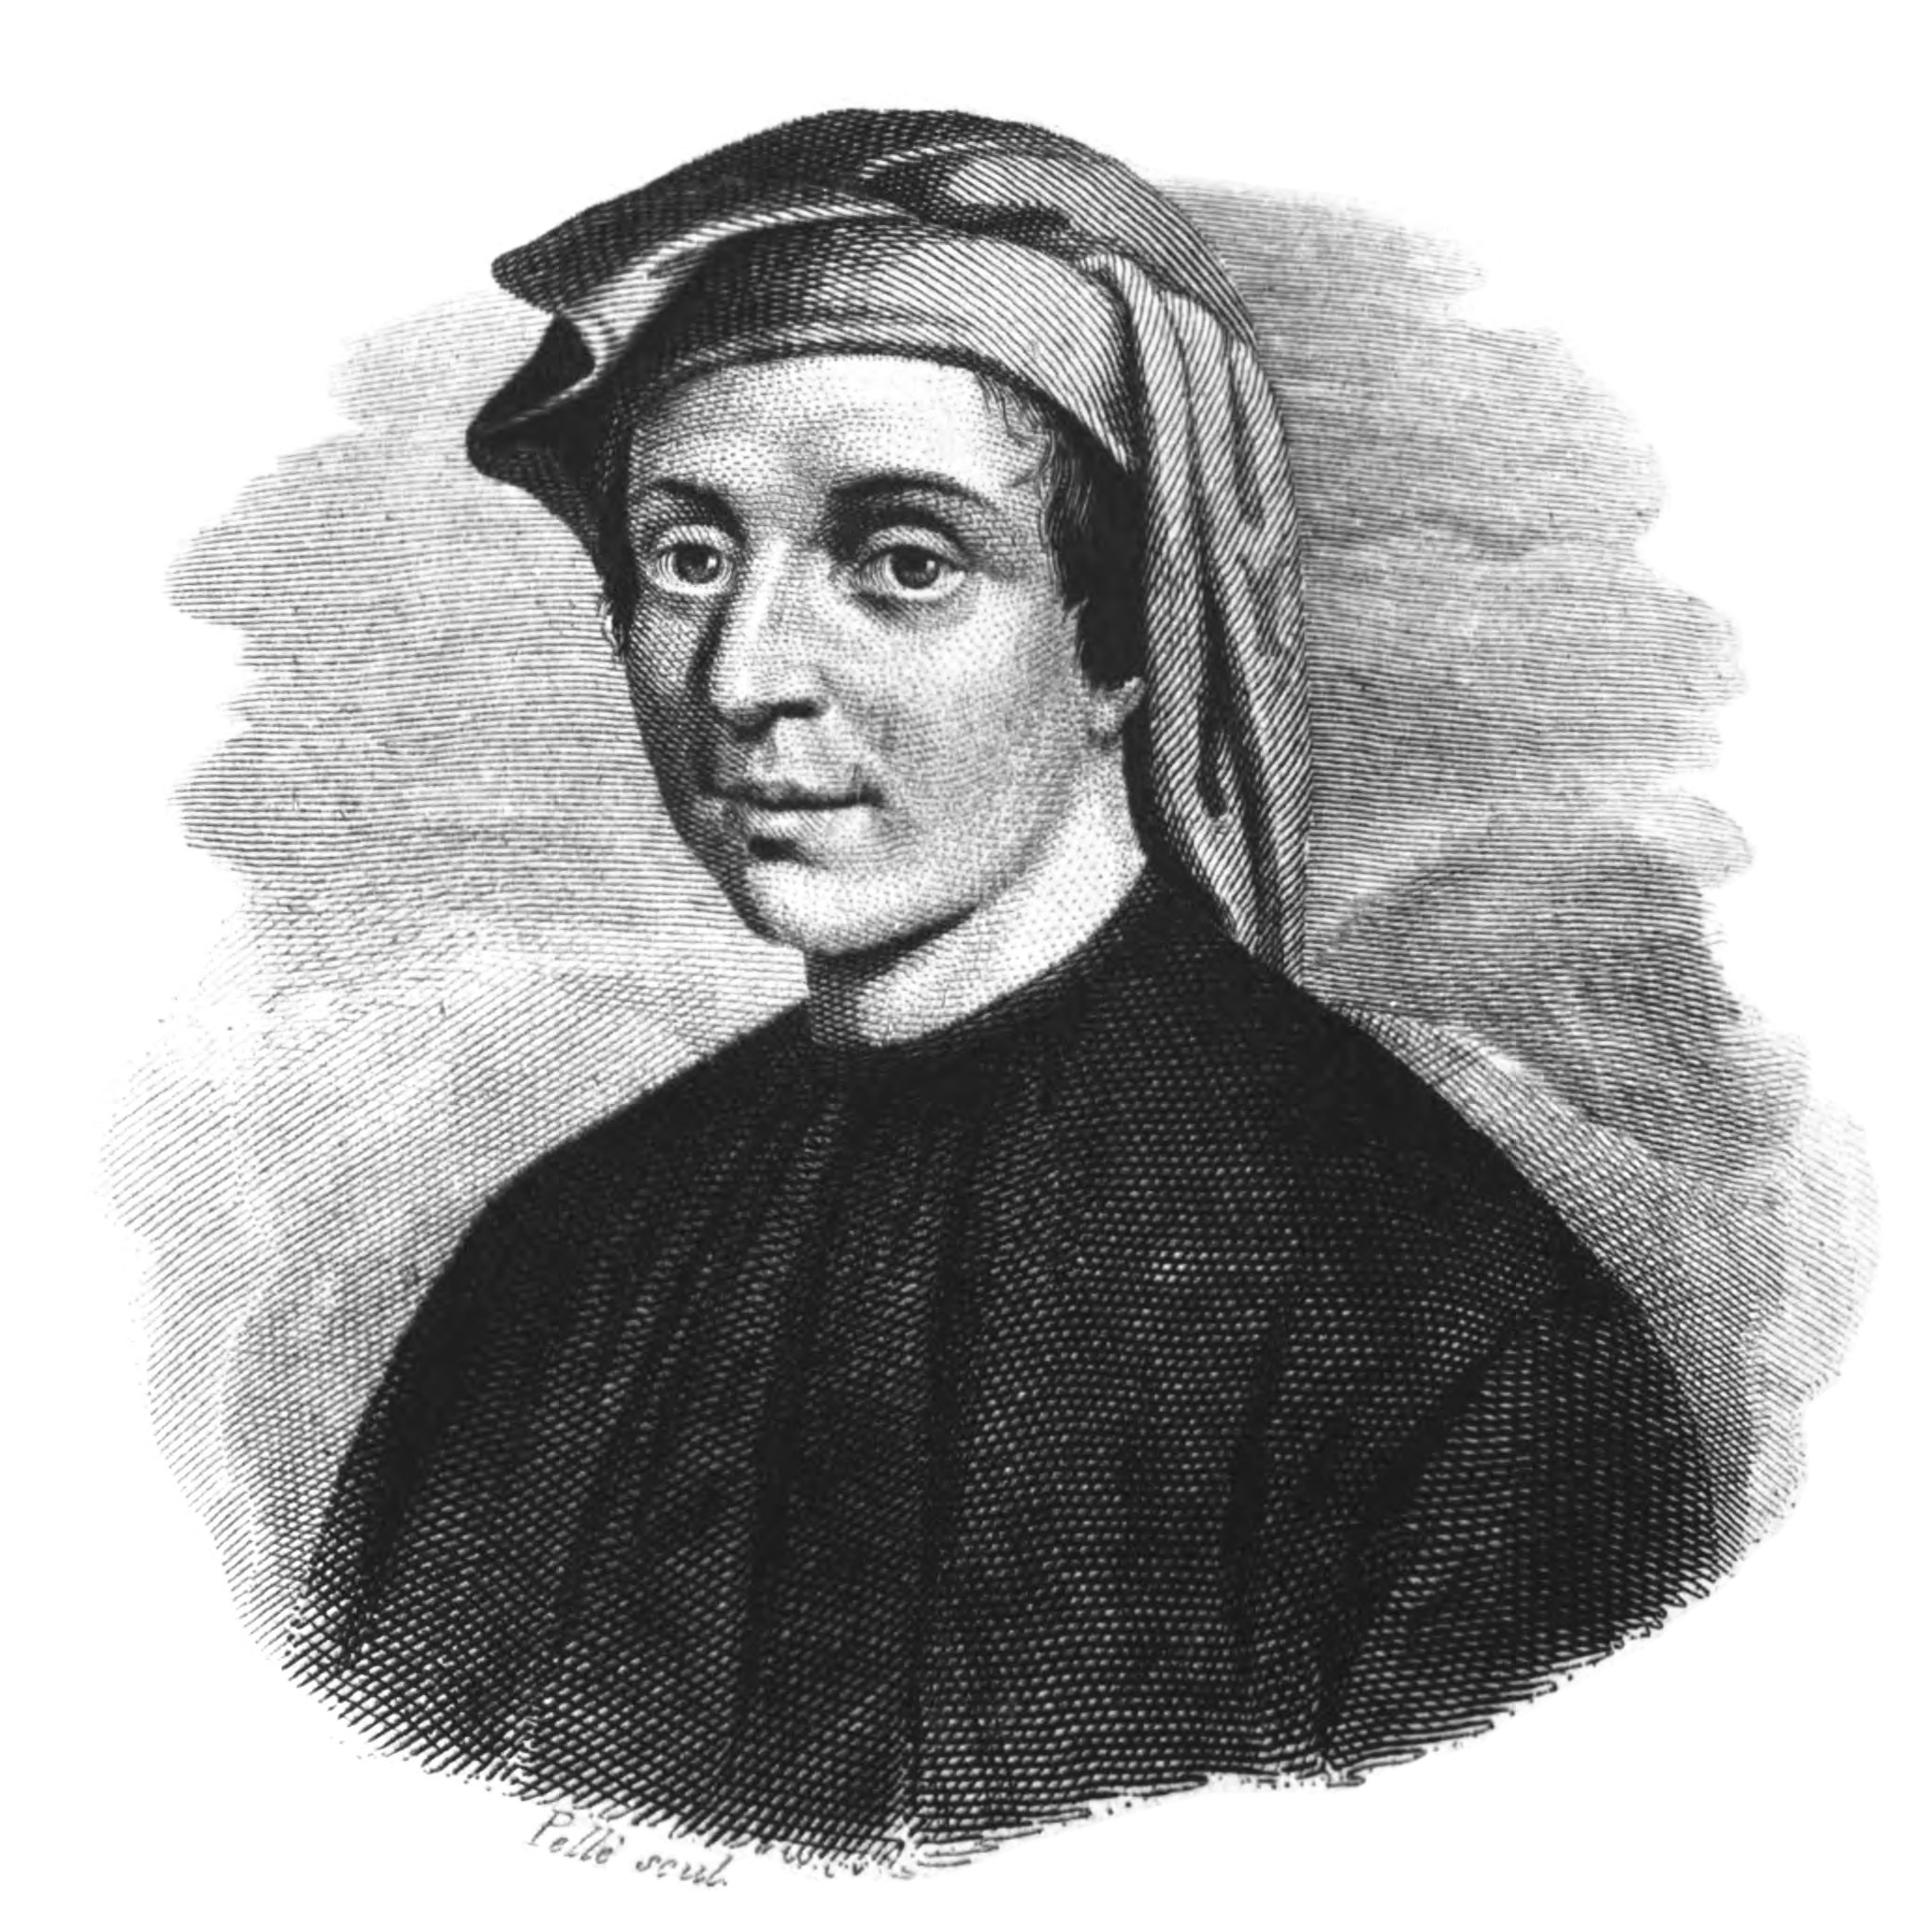
\includegraphics[width=0.38\textwidth,alt={Pen drawing if Leonardo Fibonacci}]{figures/Fibonacci.jpg}%
    };
  \end{tikzpicture}
  \caption[Leonardo Pisano]{\sloppy{Leonardo Pisano.}}
  \label{fig:frederick}
\end{figure}
The Euclidean parametrization of the Pythagorean triples has some further applications, but in order to get there we must make a short excursion to the city of Pisa in the 13\supth{} century, where Frederick~II reigned as the Holy Roman Emperor, and King of Sicily, Jerusalem, and Apulia. When Leonardo Pisano, more commonly known as Fibonacci, was summoned to the court of Frederick~II, he met with Master John of Palermo who challenged him with mathematical problems.

One of the challenges of Master John is stated as follows: Find a rational number $q$ such that the numbers
\begin{equation*}
  q^2-5 \qquad\text{and}\qquad q^2+5
\end{equation*}
are both squares of rational numbers. Fibonacci's investigations into this problem would eventually lead him to write his \emph{Liber Quadratorum} \cite{fibonacci1987}. The Liber Quadratorum covers topics such as Pythagorean triples, a method of generating infinitely many of them, and arithmetic progressions of squares. There were no known remaining copies of the Liber Quadratorum until a 15\supth{} century copy was rediscovered in the Biblioteca Ambrosiana in Milan, which was republished in print in 1857 by the Italian historian and mathematician Baldassarre Boncompagni Ludovisi. Today, the work available in an English translation by Laurence E.~Sigler as \emph{The Book of Squares} \cite{fibonacci1987}.

Master John's challenge is equivalently formulated as the question of finding four integers $a$, $b$, $c$, and $t$ such that
\begin{equation*}
  b^2-a^2=5t^2\qquad\text{and}\qquad c^2-b^2=5t^2.
\end{equation*}
Thus, we are looking for three squares $a^2$, $b^2$, and $c^2$ increasing in increments of $5t^2$. Thus we see that we can conveniently state the problem in terms of arithmetic triples of squares.

\begin{definition}
  An \define{arithmetic triple of squares} is a triple $(a^2,b^2,c^2)$ consisting of integer squares such that
  \begin{equation*}
    b^2-a^2=c^2-b^2.
  \end{equation*}
  This common increment is called the \define{congruum} and is denoted by $\Delta_{a,b,c}$, or simply $\Delta$. An arithmetic triple of squares $(a^2,b^2,c^2)$ is said to be \define{primitive} if $\gcd(a,b,c)=1$.
\end{definition}

It follows immediately from the definition that if $(a^2,b^2,c^2)$ is a primitive arithmetic triple of squares, then $a$, $b$, and $c$ are also pairwise relatively prime.

We are thus looking for an arithmetic triple of squares, with a congruum of the form $\Delta:=5t^2$. In \zcref{exercise:div-increment-a-p-squares} you were asked to show that the congruum $\Delta$ of an arithmetic triple of squares is always divisible by $24$, which Fibonacci also reported on in Liber Quadratorum. We conclude from this observation that if $\Delta$ is of the form $5t^2$ then $\Delta$ must be a multiple of $2\cdot3\cdot 5 \cdot 24=720$.

\begin{figure}[t]
  \centering
  \resizebox{\textwidth}{!}{
    \begin{tikzpicture}
      \pgfmathdeclarefunction{dn}{1}{%
        \pgfmathparse{mod(#1,2)==1 ? #1 : int(#1/2)}%
      }

      \pgfmathtruncatemacro{\rmax}{9}
      \pgfmathtruncatemacro{\cwidth}{2*\rmax-1}

      \foreach \row in {1,...,\rmax} {%
        
        \pgfmathsetmacro\y{(\row-1)*sqrt(3)/2}%
        
        \pgfmathtruncatemacro\maxc{\cwidth-(\row-1)}%

        \foreach \col in {1,...,\maxc} {%
          \pgfmathtruncatemacro\nodeSum{0}%
          \pgfmathtruncatemacro\limit{\row-1}%
          
          \foreach \J in {0,...,\limit} {%
            \pgfmathtruncatemacro\term{dn(\col+\J)}%
            \pgfmathtruncatemacro\nodeSum{\nodeSum+\term}%
            \global\let\nodeSum=\nodeSum %
          }%
          
          \node[draw,thick,circle,minimum size=6mm,inner sep=0pt,align=center,font=\small]
            (nC\col R\row) at ({(\col-1)+(\row-1)/2},\y) {$\nodeSum$};%
        }%
          
        \foreach \col in {1,...,\maxc} {
          \pgfmathtruncatemacro{\ncol}{\col+1}
          \pgfmathtruncatemacro{\prow}{\row-1}
          
          \ifnum\row>1\relax
            \draw[thick] (nC\col R\row) -- (nC\col R\prow);%
            \draw[thick] (nC\col R\row) -- (nC\ncol R\prow);%
          \fi
        }%
      }%
      
      \foreach \base in {0,...,\cwidth} {%
        \pgfmathsetmacro\y{(-1)*sqrt(3)/2}
        \pgfmathtruncatemacro\pmone{isodd(\base) ? -1 : 1}
        \pgfmathtruncatemacro\half{int((\base+1)/2)}
        \pgfmathtruncatemacro\rootval{6*\half + \pmone}
        
        \node[draw,thick,rectangle,minimum size=5.5mm,inner sep=0pt,align=center,font=\small] (b\base) at ({\base-1/2},\y) {$\rootval$};
        \pgfmathtruncatemacro{\leftcol}{\base}
        \pgfmathtruncatemacro{\rightcol}{\base+1}
        \ifnum\base<\cwidth\relax
          \draw[thick] (b\base) -- (nC\rightcol R1);
        \fi
        \ifnum\base>0\relax
          \draw[thick] (b\base) -- (nC\leftcol R1);
        \fi
      }
      
      \begin{scope}[on background layer]
        \fill[CornflowerBlue] (nC1R1) circle (3mm);
        \fill[YellowOrange] (nC2R1) circle (3mm);
        \fill[CornflowerBlue] (nC3R2) circle (3mm);
        \fill[YellowOrange] (nC5R1) circle (3mm);
        \fill[CornflowerBlue] (nC3R3) circle (3mm);
        \fill[YellowOrange] (nC6R2) circle (3mm);
        \fill[CornflowerBlue] (nC6R3) circle (3mm);
        \fill[YellowOrange] (nC9R2) circle (3mm);
        \fill[CornflowerBlue] (nC1R9) circle (3mm);
        \fill[YellowOrange] (nC10R4) circle (3mm);
        \fill[CornflowerBlue] (nC8R5) circle (3mm);
        \fill[YellowOrange] (nC13R3) circle (3mm);
        \fill[CornflowerBlue] (nC11R3) circle (3mm);
        \fill[YellowOrange] (nC14R3) circle (3mm);
      \end{scope}
    \end{tikzpicture}
  }
  \caption[Differences of squares congruent to $1$ modulo $24$]{The numbers in squares at the base of the grid are the numbers of the form $6m\pm 1$, which correspond exactly to all the numbers $n$ such that $n^2-1$ is divisible by $24$. If $x$ and $y$ are two numbers in squares at the base of the grid, then the number $k$ at the apex of the triangle spanned by $x$ and $y$ satisfies $y^2-x^2=k\cdot 24$. For each primitive arithmetic triple $(x^2,y^2,z^2)$ of squares, the apex of the triangle spanned by $x$ and $y$ is marked in blue, and the apex of the triangle spanned by $y$ and $z$ is marked in orange.}
  \label{figure:quotients-of-differences-of-squares}
\end{figure}

% \begin{figure}[t]
%   \centering
%   \resizebox{\textwidth}{!}{
%     \begin{tikzpicture}
%       \pgfmathdeclarefunction{dn}{1}{%
%         \pgfmathparse{mod(#1,2)==1 ? #1 : int(#1/2)}%
%       }

%       \pgfmathtruncatemacro{\rmax}{9}
%       \pgfmathtruncatemacro{\cwidth}{2*\rmax-1}
%       % Loop over rows
%       \foreach \row in {1,...,\rmax} {%
        
%         % Vertical position
%         \pgfmathsetmacro\y{(\row-1)*sqrt(3)/2}%
        
%         % Columns shrink by one each row up
%         \pgfmathtruncatemacro\maxc{\cwidth-(\row-1)}%

%         \foreach \col in {1,...,\maxc} {%
%           \pgfmathtruncatemacro\S{0}%
%           \pgfmathtruncatemacro\J{0}%
%           \pgfmathtruncatemacro\limit{\row}%
%           \pgfmathloop
%           \ifnum\J<\limit\relax
%             \pgfmathtruncatemacro\term{dn(\col+\J)}%
%             \pgfmathtruncatemacro\S{\S+\term}%
%             \pgfmathtruncatemacro\J{\J+1}%
%             \repeatpgfmathloop
%             \node[draw,thick,circle,minimum size=6mm,inner sep=0pt,align=center,font=\small]
%               (nC\col R\row) at ({(\col-1)+(\row-1)/2},\y) {\S};%
%             }%
          
%         \foreach \col in {1,...,\maxc} {
%           \pgfmathtruncatemacro{\ncol}{\col+1}
%           \pgfmathtruncatemacro{\prow}{\row-1}
          
%           \ifnum\row>1\relax
%             \draw[thick] (nC\col R\row) -- (nC\col R\prow);%
%             \draw[thick] (nC\col R\row) -- (nC\ncol R\prow);%
%           \fi
%         }%
%       }%
      
%       \foreach \base in {0,...,\cwidth} {%
%         \pgfmathsetmacro\y{(-1)*sqrt(3)/2}
%         \pgfmathtruncatemacro\pmone{\ifodd\base -1\else 1\fi}
%         \pgfmathtruncatemacro\half{int((\base+1)/2)}
%         \pgfmathtruncatemacro\rootval{6*\half + \pmone}
        
%         \node[draw,thick,rectangle,minimum size=5.5mm,inner sep=0pt,align=center,font=\small] (b\base) at ({\base-1/2},\y) {\rootval};
%         \pgfmathtruncatemacro{\leftcol}{\base}
%         \pgfmathtruncatemacro{\rightcol}{\base+1}
%         \ifnum\base<\cwidth
%           \draw[thick] (b\base) -- (nC\rightcol R1);
%         \fi
%         \ifnum\base>0
%           \draw[thick] (b\base) -- (nC\leftcol R1);
%         \fi
%       }
      
%       \begin{scope}[on background layer]
%         \fill[CornflowerBlue] (nC1R1) circle (3mm);
%         \fill[YellowOrange] (nC2R1) circle (3mm);
%         \fill[CornflowerBlue] (nC3R2) circle (3mm);
%         \fill[YellowOrange] (nC5R1) circle (3mm);
%         \fill[CornflowerBlue] (nC3R3) circle (3mm);
%         \fill[YellowOrange] (nC6R2) circle (3mm);
%         \fill[CornflowerBlue] (nC6R3) circle (3mm);
%         \fill[YellowOrange] (nC9R2) circle (3mm);
%         \fill[CornflowerBlue] (nC1R9) circle (3mm);
%         \fill[YellowOrange] (nC10R4) circle (3mm);
%         \fill[CornflowerBlue] (nC8R5) circle (3mm);
%         \fill[YellowOrange] (nC13R3) circle (3mm);
%         \fill[CornflowerBlue] (nC11R3) circle (3mm);
%         \fill[YellowOrange] (nC14R3) circle (3mm);
%       \end{scope}
%     \end{tikzpicture}
%   }
%   \caption[Differences of squares congruent to $1$ modulo $24$]{The numbers in squares at the base of the grid are the numbers of the form $6m\pm 1$, which correspond exactly to all the numbers $n$ such that $n^2-1$ is divisible by $24$. If $x$ and $y$ are two numbers in squares at the base of the grid, then the number $k$ at the apex of the triangle spanned by $x$ and $y$ satisfies $y^2-x^2=k\cdot 24$. For each primitive arithmetic triple $(x^2,y^2,z^2)$ of squares, the apex of the triangle spanned by $x$ and $y$ is marked in blue, and the apex of the triangle spanned by $y$ and $z$ is marked in orange.}
%   \label{figure:quotients-of-differences-of-squares}
% \end{figure}

The fact that the congruum in an arithmetic triple of squares is always a multiple of $24$ implies that primitive arithmetic triples of squares consist entirely of integers of the form $(6m\pm 1)^2$. Any such square exceeds a multiple of $24$ by one. This significantly reduces the search space for arithmetic triples of squares. If $a_n$ is the $n$\supth{} positive integer of the form $(6k\pm 1)^2$, then
\begin{equation*}
  d_n:=\frac{a_{n+1}-a_n}{24}=
  \begin{cases}
    n & \text{if $n$ is odd,}\\
    n/2 & \text{if $n$ is even.}
  \end{cases}
\end{equation*}
In order to determine the number of units of $24$ in the difference between two arbitrary numbers of the form $(6m\pm 1)^2$, we simply sum the numbers $d_n$: We define
\begin{equation*}
  s_{n,m}:=\sum_{i=0}^md_{n+i}=\frac{a_{n+m+1}-a_n}{24}.
\end{equation*}
Alternatively, the numbers $s_{n,m}$ are determined by the recursive rule $s_{n,m}=s_{n+1,m-1}+s_{n,m-1}-s_{n+1,m-2}$.
The numbers $s_{n,m}$ are displayed in \zcref{figure:quotients-of-differences-of-squares}, from which we determine that:
    \begin{align*}
      5^2-1^2 & = 7^2-5^2 & & = 1\cdot 24, \\
      13^2 - 7^2 & = 17^2 - 13^2 & & = 5\cdot 24, \\
      17^2 - 7^2 & = 23^2 - 17^2 & & = 10\cdot 24, \\
      25^2 - 17^2 & = 31^2 - 25^2 & & = 14\cdot 24, \\ 
      29^2 - 1^2 & = 41^2 - 29^2 & & = 35\cdot 24, \\
      37^2 - 23^2 & = 47^2 - 37^2 & & = 35\cdot 24, \\
      41^2 - 31^2 & = 49^2 - 41^2 & & = 30\cdot 24.
    \end{align*}
The solution to Master John's problem to Fibonacci, which Fibonacci reported in Proposition 17 of \emph{Liber Quadratorum}, thus corresponds to the last listed arithmetic triple of squares, which gives
\begin{equation*}
  \left(\frac{41}{12}\right)^2-\left(\frac{31}{12}\right)^2=\left(\frac{49}{12}\right)^2-\left(\frac{41}{12}\right)^2=5.
\end{equation*}

% \begin{proposition}
%   If $a$, $b$, and $c$ are integers such that
%   \begin{equation*}
%     \Delta:=b^2-a^2=c^2-b^2,
%   \end{equation*}
%   then $24\mid \Delta$.
% \end{proposition}

% \begin{proof}
%   We will prove separately that $\Delta$ is of the form $8k$ and of the form $3k$. Recall that even squares are of the form $4k$, while odd squares are of the form $8k+1$, implying that differences of squares cannot be of the form $4k+2$. Since both $\Delta$ and $2\Delta$ occur as the difference of squares, where $2\Delta=c^2-a^2$, it follows that $\Delta$ must be of the form $4k$.

%   It follows that $a^2$, $b^2$, and $c^2$ are either all even or all odd. By dividing out any common factors of $a^2$, $b^2$, and $c^2$ we may assume that they are all odd, which implies that $\Delta$ is a multiple of $8$.

%   To see that $\Delta$ is a multiple of $3$, recall that all odd squares are of the form $36k+9$ or $12k+1$, so that differences of odd squares are of the form $12k$, $12k+8$, or $12k+10$. Since $\Delta=b^2-a^2$ can only be of the form $12k+8$ if $b\equiv \pm{1}\pmod{6}$ and $a\equiv 3\pmod 6$, there cannot be a square $c^2$ such that $c^2-b^2$ is also of the form $12k+8$. Likewise we rule out $12k+10$ from the possible options for $\Delta$. Thus, we conclude that $\Delta$ is a multiple of $12$, and in particular it is a multiple of $3$.
% \end{proof}

Arithmetic triples of squares are closely related to Pythagorean triples. Given an arithmetic triple of squares $(a^2,b^2,c^2)$, we can write $b^2$ as a sum of two squares written in terms of $a$ and $c$. The crucial identity that leads to the construction of a Pythagorean triple using the integers $a$, $b$, and $c$ is
\begin{equation*}
  c^2+a^2=2b^2.
\end{equation*}
Using this identity, we see that
\begin{equation*}
  \frac{(c-a)^2}{4}+\frac{(c+a)^2}{4}= \frac{c^2-2ac+a^2}{4}+\frac{c^2+2ac+a^2}{4} = \frac{c^2+ a^2}{2} = b^2.
\end{equation*}
Thus, if $(a^2,b^2,c^2)$ is an arithmetic progression of squares, then the integers
\begin{equation*}
  x := \frac{c-a}{2},\qquad y:= \frac{c+a}{2},\qquad\text{and}\qquad z:= b
\end{equation*}
determine a Pythagorean triple $(x,y,z)$. Conversely, if $(x,y,z)$ is a Pythagorean triple, then we define
\begin{equation*}
  a := \abs{y-x}, \qquad b := z,\qquad\text{and}\qquad c:= y+x,
\end{equation*}
so that $(a^2,b^2,c^2)$ is easily seen to be an arithmetic triple of squares. Here, we defined $a$ to be the \emph{distance} between $y$ and $x$ in order to ensure that $a$ is positive. The congruum of this arithmetic triple is given by
\begin{equation*}
  z^2-(y-x)^2=2xy,
\end{equation*}
which is four times the area of the Pythagorean triangle described by the Pythagorean triple $(x,y,z)$.
The operations thus described create the following correspondence between some of the most familiar arithmetic triples of squares and Pythagorean triples:
\begin{align*}
  (1^2,5^2,7^2)   & \bimapsto (3,4,5), \\
  (7^2,13^2,17^2) & \bimapsto (5,12,13), \\
  (1^2,29^2,41^2) & \bimapsto (21,20,29), \\
  (7^2,17^2,23^2) & \bimapsto (15,8,17).
\end{align*}
The fact that these operations mapping arithmetic triples of squares to Pythagorean triples and back are mutually inverse to each other is easily verified by a few quick computations, which we leave to the reader. Thus, we have established:

\begin{theorem}\label{theorem:correspondence-arithmetic-triples-squares}
  Arithmetic triples $(a^2,b^2,c^2)$ of squares are in bijective correspondence with Pythagorean triples $(x,y,z)$, so that primitive arithmetic triples of squares correspond to primitive Pythagorean triples.
\end{theorem}

\begin{proof}
  We only prove that $(a^2,b^2,c^2)$ is a primitive arithmetic triple of squares if and only if the Pythagorean triple
  \begin{equation*}
    \left(\frac{c-a}{2},\frac{c+a}{2},b\right)
  \end{equation*}
  is primitive.

  For the forward direction, assume that $\gcd(a,b,c)=1$. To see that $(c-a)/2$ and $(c+a)/2$ are relatively prime, it suffices to show that any common divisor $d$ of $c-a$ and $c+a$ is a divisor of $2$. Indeed, if $d$ is a common divisor of $c-a$ and $c+a$, then it is also a common divisor of $2a=(c+a)-(c-a)$ and $2c=(c+a)+(c-a)$. Since $a$ and $c$ are relatively prime, it follows that $d$ is a divisor of $2$.

  Likewise, to show that $(c-a)/2$ and $b$ are relatively prime, we note that since $b$ is odd it suffices to show that $c-a$ and $b$ are relatively prime, which is only the case if $(c-a)^2$ and $b^2$ are relatively prime. This follows from
  \begin{equation*}
    (c-a)^2=c^2+a^2-2ac=2b^2-2ac,
  \end{equation*}
  since any common divisor of $(c-a)^2$ and $b^2$ is also a common divisor of $b^2$ and $2ac$, which are relatively prime by assumption. The proof that $(c+a)/2$ and $b$ are relatively prime is similar. 

  For the reverse direction, assume that
  \begin{equation*}
    \left(\frac{c-a}{2},\frac{c+a}{2},b\right)
  \end{equation*}
  is a primitive Pythagorean triple, so that $b$ is odd, and thus $b$, $(c-a)/2$, and $(c+a)/2$ are all pairwise relatively prime. Then any common divisor $d$ of $a$ and $c$ is also a common divisor of $(c-a)/2$ and $(c+a)/2$, so that $a$ and $c$ are seen to be relatively prime.

  We will prove that $(x,y,z)$ is a primitive Pythagorean triple if and only if
  \begin{equation*}
    ((y-x)^2,z^2,(y+x)^2)
  \end{equation*}
  is a primitive arithmetic triple of squares. By Euclid's parametrization of Pythagorean triples, it suffices to show that for any two
\end{proof}

The previous theorem raises an interesting point. Since the primitive Pythagorean triples are precisely described by Euclid's parametrization, there must similarly be a parametrization of the arithmetic triples of squares.

\begin{corollary}
  For any primitive arithmetic triple of squares $(a^2,b^2,c^2)$, we can uniquely determine two relatively prime positive integers $s<t$ of opposite parity such that
  \begin{equation*}
    a=2st-t^2+s^2,\qquad b=t^2+s^2,\qquad\text{and}\qquad c=2st+t^2-s^2
  \end{equation*}
  with common difference $d= 2st(t-s)^2$.
\end{corollary}

\exercises

\begin{starter}
  \exercise \emph{Bhaskara's proof of the Pythagorean Theorem.} Use the following diagram to give a proof of \zcrefnamed{theorem:pythagorean-theorem}:
  \begin{figure}[H]
    \centering
    \begin{tikzpicture}[scale=.0625,thick,line join=round,line cap=round]
      \pgfmathsetmacro{\myangle}{atan(28/45)}
      \draw (0,0) rectangle (53,53);
      \foreach \k/\x/\y in {0/0/0, 1/53/0, 2/53/53, 3/0/53}
      \draw (\x,\y) -- ++({\myangle + 90*\k}:45);
    \end{tikzpicture}
  \end{figure}
  
\end{starter}

\begin{routine}
  \exercise \label{exercise:brahmagupta-fibonacci-identity}\emph{The Brahmagupta--Fibonacci identity.} Show that
  \begin{equation*}
    (a^2+b^2)(c^2+d^2)=(ac\pm bd)^2 + (ad\mp bc)^2.
  \end{equation*}
  Conclude that if $m$ and $n$ are two integers that can be written as the sum of two squares, then their product $mn$ can also be written as the sum of two squares.
  \exercise \label{exercise:divisibility-legs-pythagorean-triples}Consider a primitive Pythagorean triple $(x,y,z)$.
  \begin{subexenum}
  \item Prove that exactly one of $x$, $y$, and $z$ is divisible by $3$.
  \item Prove that exactly one of $x$, $y$, and $z$ is divisible by $5$.
  \item Find all Pythagorean triples $(x,y,z)$ in which $x=30$ or $y=30$. Can any of them be primitive?
    % (30,16,34),
    % (30,40,50),
    % (30,72,78),
    % (30,224,226)
  \item Find all relatively prime positive integers $x$ and $z$ such that
    \begin{equation*}
      x^2+60^2=z^2,
    \end{equation*}
    showing that the components divisible by $3$, $4$, or $5$ might all coincide.
    % (11,60,61),
    % (91,60,109),
    % (221,60,229),
    % (899,60,901).
  \end{subexenum}
  \exercise Find three distinct triangular numbers in an arithmetic progression.
  \exercise Find three distinct tetrahedral numbers, that is, numbers of the form $\binom{n+2}{3}$, in an arithmetic progression.  
  \exercise Define an \define{Egyptian triple} to be a triple $(a,b,c)$ of integers such that
  \begin{equation*}
    \frac{1}{a}+\frac{1}{b}=\frac{1}{c}.
  \end{equation*}
  Such an Egyptian triple is called \define{primitive} if $\gcd(a,b)=1$.
  \begin{enumerate}
  \item Show that if $(a,b,c)$ is a primitive Egyptian triple, then $\gcd(a,c)=\gcd(b,c)=1$.
  \item Show that for any primitive Egyptian triple $(a,b,c)$ with $a\leq b$, we can uniquely determine two relatively prime positive integers $s\leq t$ such that
    \begin{equation*}
      a=s(s+t),\qquad b=t(s+t),\qquad c=st.
    \end{equation*}
  \end{enumerate}
\end{routine}

\begin{challenge}
  \exercise Find a parametrization of all pairs $(m,n)$ of natural numbers such that $n^2-m^2$ is a number of the form $2^k$, and prove that your parametrization is a bijection.
  \exercise Find a complete parametrization of all triples $(a,b,c)$ satisfying $\gcd(a,b,c)=1$ such that
    \begin{equation*}
      \frac{1}{a^2}+\frac{1}{b^2}=\frac{1}{c^2}.
    \end{equation*}
    Note: The condition $\gcd(a,b,c)=1$ does not imply that $a$, $b$, and $c$ are pairwise relatively prime.
  \exercise Show that for every positive integer $y$ divisible by $4$, there is a primitive Pythagorean triple $(a,b,c)$ with $b=y$.
  \exercise Show that every odd positive integer $x\geq 3$ can be written in the form $t^2-s^2$, where $s<t$ are relatively prime positive integers of opposite parity. Conclude that every odd integer $x\geq 3$ occurs in a Pythagorean triple $(a,b,c)$ with $a=x$.
  \exercise Define
  \begin{align*}
    x_n & := F_n F_{n+1}+(-1)^n, \\
    y_n & := 2F_nF_{n+1}, \\
    z_n & := F_{n}^2+F_{n+1}^2,
  \end{align*}
  where $F_k$ is the $k$\supth{} Fibonacci number. Show that $(x_n,y_n,z_n)$ is a Pythagorean triple for each $n$.
  \exercise Let
  \begin{align*}
    a_n & := F_{n}F_{n+1}- (-1)^n, \\
    b_n & := F_{n}^2 + F_{n+1}^2, \\
    c_n & := 3F_{n}F_{n+1}+(-1)^{n}.
  \end{align*}
  be defined as in \zcref{exercise:arithmetic-progression-fibonacci}, so that $(a_n^2,b_n^2,c_n^2)$ is an arithmetic triple of squares. Show that
  \begin{equation*}
    \gcd(a_n,b_n,c_n)=
    \begin{cases}
      2 & \text{if $n\equiv 1\pmod{3}$,}\\
      1 & \text{otherwise.}
    \end{cases}
  \end{equation*}
    \exercise Consider three squares $a^2$, $b^2$, and $c^2$ in an arithmetic progression in increasing order.
  \begin{subexenum}
  \item Show that at least one of
    \begin{equation*}
      c-b,~c-a,~\text{and}~b-a
    \end{equation*}
    is divisible by $3$.
  \item Show that at least one of
    \begin{equation*}
      c-b,~c-a,~\text{and}~b-a
    \end{equation*}
    is divisible by $4$.
  \item Show that at least one of
    \begin{equation*}
      b~\text{and}~c-a
    \end{equation*}
    is divisible by $5$.
  \item Find all arithmetic progressions $(a^2,b^2,c^2)$ such that $c-a=60$, where only $a$ is allowed to be negative. Are there any such triples with $\gcd(a,b,c)=1$?
    % (-14,34,46),
    % (10,50,70),
    % (42,78,102),
    % (194,226,254)
  \item Find all \emph{primitive} arithmetic progressions $(a^2,b^2,c^2)$ such that $c-a=120$, where only $a$ is allowed to be negative. Hint: There are four such triples.
    % (-49,61,71)
    % (31,109,151)
    % (161,229,281)
    % (839,901,959)
  \end{subexenum}
  \exercise Find all solutions to the equation $x^2-2y^2=1$.
  \exercise \emph{Master Theodore's problem for Leonardo Pisano} \cite[Proposition 24]{fibonacci1987}. Find three positive integers $x$, $y$, and $z$ such that the numbers
  \begin{equation*}
    x+y+z+x^2,\qquad x+y+z+x^2+y^2,\qquad\text{and}\qquad x+y+z+x^2+y^2+z^2
  \end{equation*}
  are all squares.
  \exercise Consider a quadruple $(a,b,c,d)$ such that $\gcd(a,b,c,d)=1$ and
  \begin{equation*}
    a^2+b^2+c^2=d^2.
  \end{equation*}
  Prove that there is a unique quadruple $(s,t,u,v)$ such that $\gcd(s,t,u,v)=1$, the numbers $s^2+t^2$ and $u^2+v^2$ have opposite parity, and
  \begin{align*}
    a & = 2(su-tv), \\
    b & = 2(sv+tu), \\
    c & = s^2+t^2-u^2-v^2, \\
    d & = s^2+t^2+u^2+v^2.
  \end{align*}
\end{challenge}

%%% Local Variables:
%%% mode: latex
%%% TeX-master: "number-theory"
%%% TeX-engine: luatex
%%% End:


\chapter{Infinite Descent}

\section{The Method of Infinite Descent}

The method of infinite descent was invented by Fermat. He used this method effectively to solve various problems, including that there are no solutions to $x^4+y^4=z^4$ in the positive integers, and that the area of a right triangle is not a perfect square. The method of infinite descent is used to show that certain properties or identities are impossible, by showing that if they do hold then an infinitely descending sequence of natural numbers can be constructed. The following theorem shows that there is no such sequence.

\begin{proposition}\label{proposition:infinite-descent}
  There is no infinite descending sequence
  \begin{equation*}
    a_0 > a_1 > a_2 > \cdots
  \end{equation*}
  of natural numbers.
\end{proposition}

\begin{proof}
  Suppose, by way of contradiction, that there is such a sequence
  \begin{equation*}
    a_0 > a_1 > a_2 > \cdots.
  \end{equation*}
  Then the set
  \begin{equation*}
    A:=\{a_0,a_1,a_2,\ldots\}
  \end{equation*}
  is a nonempty subset of the natural numbers, and by \zcrefnamed{theorem:well-ordering-natural-numbers} it follows that this set has a least element. However, all the elements in $A$ are of the form $a_n$ for some natural number $\mathbb{N}$, and none of these elements are minimal, since we have assumed that $a_n>a_{n+1}$. This contradiction shows that our assumption that there exists an infinite descending sequence must be false, and thus there is no such sequence.
\end{proof}

The previous proposition leads to Fermat's method of infinite descent. Fermat observed that if an assumption $H$ leads to an infinite descending sequence, then the assumption $H$ must be false. 

\begin{theorem}[Method of Infinite Descent]\label{theorem:method-of-descent}
  Consider a set $A$ equipped with a function $f:A\to A$ and a function $h:A\to\mathbb{N}$. If $h(f(a))<h(a)$ for all $a$, then $A$ is empty.
\end{theorem}

\begin{proof}
  Suppose, by way of contradiction, that the set $A$ is inhabited by an element $a\in A$. By iterating $f$, we define a sequence of elements $a_i$ by
  \begin{align*}
    a_0 & := a \\
    a_{i+1} & := f(a_i).
  \end{align*}
  Then we have $h(a_0)>h(a_i)>h(a_2)>\cdots$, which is an infinite descending sequence of natural numbers. Thus, the assumption that $A$ is inhabited was false.
\end{proof}

In \zcref{section:vieta-jumping} we used Vieta jumping to jump between rational points on the unit circle in such a way that the common denominators formed a decreasing sequence of positive integers. Necessarily, this process terminates once an integral point on the unit circle is reached. Vieta jumping can also be used with the method of infinite descend.

Recall that the basic idea of Vieta jumping is to use Vi\`ete's formulas for the roots of a quadratic formula
\begin{equation*}
  (x-r)(x-s)=x^2-(r+s)x+rs
\end{equation*}
in order to jump to the other root once one is known.
We saw in \zcref{theorem:vieta-formulas-quadratic} that if $r$ is a root of a monic polynomial $x^2-Bx+C$, then the other root $s$ satisfies
\begin{equation*}
  s=B-r=\frac{C}{s}.
\end{equation*}
Thus, if we know one root of a quadratic polynomial then we can easily `jump' to the other root using one the above formulas. Vieta jumping became a popular problem-solving technique for international contests such as the International Mathematics Olympiad.

\begin{example}
  In \zcref{exercise:div-product-sum-of-squares} you were asked to show that for any two positive integers $x$ and $y$ such that $xy\mid x^2+y^2$, we must have $x=y$. The expected solution was to observe that the discriminant of the quadratic equation $x^2-kxy+y^2=0$ seen as an equation in one variable $x$ and a parameter $y$ is $(ky)^2-4y^2$, which is a square if and only if $k=2$. Although this problem can readily be solved directly, we will use it here to illustrate Vieta jumping.

  We first observe that the quadratic equation
  \begin{equation*}
    x^2-kxy + y^2=0
  \end{equation*}
  arising from the divisibility condition $xy\mid x^2+y^2$ is \emph{homogeneous} in the sense that each of the three terms have the same degree in $x$ and $y$ combined. Thus, if $x$ an $y$ satisfy this polynomial equation, then so must
  \begin{equation*}
    x' :=\frac{x}{\gcd(x,y)}\qquad\text{and}\qquad y':=\frac{y}{\gcd(x,y)}.
  \end{equation*}
  We can therefore solve the problem by showing that the only pair of coprime positive integers $x$ and $y$ satisfying the polynomial equation must satisfy $x=y=1$.

  To see this, we may assume without loss of generality that $0<y<x$. Given that $x$ is a solution of the quadratic equation $t^2-kty+y^2$ in the variable $t$, it follows that the other solution is $x':=ky-x$. Notice that $\gcd(ky-x,y)=1$, so that $x':=ky-x$ and $y$ are again relatively prime. Furthermore, since $xx'=y^2$ it follows that
  \begin{equation*}
    0<x'=\frac{y^2}{x}<y.
  \end{equation*}
  We have thus found a new solution with $x'<y$. Now we can swap the roles for $x'$ and $y$ and repeat the process, obtaining every smaller solutions in the positive integers. Since this is clearly impossible, it must have been impossible for there to be a pair of relatively prime positive integers $x$ and $y$ such that $xy\mid x^2+y^2$.
\end{example}

\section{The Area of a Pythagorean Triangle is not a Square}

A classic application of Fermat's infinite descent gives us that the area of a Pythagorean triangle is never a square number. Recall that the area of a triangle is half the base times the height, so that every Pythagorean triple $(a,b,c)$ determines a Pythagorean triangle with area
\begin{equation*}
  \frac{1}{2}ab.
\end{equation*}

\begin{theorem}\label{theorem:is-not-square-area-pythagorean-triangle}
  The area of a Pythagorean triangle is not a square number.
\end{theorem}

\begin{proof}
  It suffices to prove the statement for primitive Pythagorean triangles; that is, a triangle whose sides $(a,b,c)$ form a primitive Pythagorean triple. By \zcrefnamed{theorem:euclids-parametrization}, we can find two relatively prime integers $s<t$ of opposite parity, such that
  \begin{equation*}
    a=t^2-s^2,\qquad b=2st,\qquad\text{and}\qquad c=t^2+s^2.
  \end{equation*}
  The area of the triangle is given in terms of this parametrization by the nonzero quantity
  \begin{equation*}
    st(t^2-s^2)=st(t-s)(t+s).
  \end{equation*}
  Now observe that all of these factors are relatively prime to one another; indeed, given that $s$ and $t$ are relatively prime, it follows at once from \zcref{proposition:gcd-euclidean-division} that both $s$ and $t$ are relatively prime to both $s-t$ and $s+t$. Furthermore, any common divisor of $s-t$ and $s+t$ must be a common divisor of $2s$ and $2t$, which implies that it must divide $2$. However, $s-t$ and $s+t$ are odd since $s$ and $t$ are of opposite parity, so that $s-t$ and $s+t$ are seen to be relatively prime. Thus we conclude that if the area of the Pythagorean triangle is a square, then each of these factors must also be a square. This allows us to write
  \begin{equation*}
    s=u^2,\quad t=v^2,\quad t-s=x^2,\quad\text{and}\quad t+s=y^2.
  \end{equation*}
  Since $s$ and $t$ are of opposite parity, it follows that $x$ and $y$ are both odd. Now notice that the triple of integers
  \begin{equation*}
    \left(\frac{y-x}{2},\frac{y+x}{2},v\right)
  \end{equation*}
  is a Pythagorean triple, since
  \begin{equation*}
    \left(\frac{y-x}{2}\right)^2+\left(\frac{y+x}{2}\right)^2=\frac{y^2+x^2}{2}=v^2.
  \end{equation*}
  Furthermore, the area of the corresponding Pythagorean triangle is given by
  \begin{equation*}
    \frac{1}{2}\left(\frac{y-x}{2}\right)\left(\frac{y+x}{2}\right)=\frac{y^2-x^2}{8}=\frac{u^2}{4}.
  \end{equation*}
  The quantity $u^2/4$ must therefore be an integer strictly less than $s$, which in turn is strictly less than the area $\frac{1}{2}ab$. Thus, we have constructed a Pythagorean triangle whose area is a strictly smaller nonzero square number, which leads to a contradiction by infinite descent.
\end{proof}

\section{The Unsolvability of \texorpdfstring{$x^4+y^4=z^4$}{x⁴ + y⁴ = z⁴}}

\begin{theorem}
  There are no three positive integers $x$, $y$, and $z$ for which the equation
  \begin{equation*}
    x^4+y^4=z^2
  \end{equation*}
  holds.
\end{theorem}

\begin{proof}
  Consider the set
  \begin{equation*}
    A:=\{(x,y,z)\in\mathbb{Z}_{>0} \mid x^4+y^4=z^2\}
  \end{equation*}
  with $h(x,y,z):=z$. We will construct a function $f:A\to A$ such that $h(f(x,y,z))<h(x,y,z)$ for every $(x,y,z)\in A$.
  
  First, we notice that if $(x,y,z)$ is a triple of positive integers satisfying the equation $x^4+y^4=z^2$, then $(x^2,y^2,z)$ is a Pythagorean triple. Since we can always divide out any common factors, we may assume that $x$ and $y$ are relatively prime. Furthermore, we may assume that $y$ is even, so that by Euclid's parametrization there are relatively prime positive integers $s<t$ of opposite parity such that
  \begin{align*}
    x^2 & = t^2-s^2, \\
    y^2 & = 2st, \\
      z & = t^2+s^2.
  \end{align*}

  The key observation is now in the first equation: We obtain a new Pythagorean triple $x^2+s^2=t^2$, allowing us to apply Euclid's parametrization of Pythagorean triples once more. Since $x$ is odd it follows that $s$ is even, so we find relatively prime positive integers $u<v$ such that
  \begin{align*}
    x & = v^2-u^2 \\
    s & = 2uv \\
    t & = v^2+u^2.
  \end{align*}
  Now it follows that $y^2 = 4uv (v^2+u^2)$. We claim that the numbers $uv$ and $v^2+u^2$ are relatively prime. To see this, note that both $u$ and $v$ are relatively prime to $v^2+u^2$ since
  \begin{equation*}
    \gcd(u,v^2+u^2)=\gcd(u,v^2)=1\qquad\text{and}\qquad\gcd(v,v^2+u^2)=\gcd(v,u^2)=1,
  \end{equation*}
  and hence their product $uv$ is also relatively prime to $v^2+u^2$.

  Since $uv$ and $v^2+u^2$ are relatively prime, the fact that $4uv(v^2+u^2)$ is a square implies that both $uv$ and $v^2+u^2$ are squares. Given that $u$ and $v$ are relatively prime, this implies that $u$ and $v$ are squares. It follows that there are integers $a$ and $b$ such that $u=a^2$ and $v=b^2$, and thus we see that
  \begin{equation*}
    v^2+u^2=a^4+b^4
  \end{equation*}
  is a square, say $c^2$. We have therefore shown that any triple of positive integers $x$, $y$, and $z$ such that $x^4+y^4=z^2$ we can construct positive integers $a$, $b$, and $c$ such that
  \begin{equation*}
    a^4 + b^4 = c^2.
  \end{equation*}
  This finishes the construction of the function $f:A\to A$. Furthermore, the strict inequality $c^2=s<s^2+t^2=z^2$ shows that $h(f(x,y,z))<h(x,y,z)$, so we conclude by \zcrefnamed{theorem:method-of-descent} that the set $A$ must be empty.
\end{proof}

\begin{corollary}
  There is no solution to the equation
  \begin{equation*}
    x^{4}+y^{4}=z^{4},
  \end{equation*}
  where $x$, $y$, and $z$ are positive integers.
\end{corollary}

\begin{proof}
  Given such a solution, set $a=x$, $b=y$, and $c=z^{2}$. Then we have
  \begin{equation*}
    a^4+b^4=c^2,
  \end{equation*}
  which is impossible.
\end{proof}

\section{Aubry's Theorem}

The following theorem is due the the French winemaker and amateur mathematician L\'eon Aubry \cite{Aubry1912}. The idea of the proof is illustrated in \zcref{figure:aubrys-theorem}.

In the proof, it will be convenient to view pairs of rational numbers $(x_1,x_2)$ as vectors. Recall that if $x=(x_1,x_2)$ and $y=(y_1,y_2)$ are vectors, then their \emph{inner product} $x\cdot y$ is defined as
\begin{equation*}
  x\cdot y := x_1y_1+x_2y_2.
\end{equation*}
In particular, $x\cdot x=x_1^2+x_2^2$ is a sum of two squares, and the equation $x\cdot x=n$ tells us that the vector $x$ lies on the circle with radius $\sqrt{n}$.

\begin{figure}[htbp]
  \centering
  \begin{tikzpicture}

    \draw[gray,very thin] (-4.1,-4.1) grid[step=1] (4.1,4.1);

    \draw[thick] (0,0) circle ({sqrt(10)});
    
    \draw[->] (-4.2,0) -- (4.2,0) node[right] {\(x\)};
    \draw[->] (0,-4.2) -- (0,4.2) node[above] {\(y\)};
    
    \coordinate (P5) at (-3,-1);
    \draw[fill=black,thick] (P5) circle (2pt);

    \coordinate (R5) at ({-1401/3305},{-10357/3305});
    \coordinate (R4) at ({1401/653},{-1517/653});
    \coordinate (R3) at ({-13/41},{129/41});
    \coordinate (R2) at ({13/5},{9/5});
    \coordinate (R1) at ({-3},{-1});
    \coordinate (Q5) at ({0},{-3});
    \coordinate (Q4) at ({2},{-2});
    \coordinate (Q3) at (0,3);
    \coordinate (Q2) at (3,2);
    \draw[DarkOrchid,very thick,->,shorten >=1.5ex] (R5) -- (R4);
    \draw[Green,very thick,->,shorten >=1ex] (R4) -- (R3);    
    \draw[YellowOrange,very thick,->,shorten >=1.5ex] (R3) -- (R2);
    \draw[CornflowerBlue,very thick,->,shorten >=1ex] (Q2) -- (R1);
    \draw[fill=white,thick] (R5) circle (2pt);
    \draw[fill=white,thick] (R4) circle (2pt);
    \draw[fill=white,thick] (R3) circle (2pt);
    \draw[fill=white,thick] (R2) circle (2pt);
    \draw[fill=DarkOrchid,draw=DarkOrchid,thick] (Q5) circle (2pt);
    \draw[fill=Green,draw=Green,thick] (Q4) circle (2pt);
    \draw[fill=YellowOrange,draw=YellowOrange,thick] (Q3) circle (2pt);
    \draw[fill=CornflowerBlue,draw=CornflowerBlue,thick] (Q2) circle (2pt);
    \draw[fill=white,thick] (R2) circle (2pt);
  \end{tikzpicture}
  \caption[Aubry's Theorem]{%
    By repeated Vieta jumping between rational points on the circle of radius $\sqrt{10}$, we always reach a point with integer coordinates. The idea of the proof is that, starting from a rational point on the circle with radius $\sqrt{n}$, if we draw a line through it and the nearest point with integer coordinates, then we find a new point on the circle with smaller common denominator.
    
    Here, we started at the point $(-1401/3305,-10357/3305)$ on the circle with radius $\sqrt{10}$. The nearest point with integer coordinates is $(0,-3)$, and the line through it intersects the circle at $(1401/653,-1517/653)$. Its nearest point with integer coordinates is $(2,-2)$. Continuing this process leads to the sequence of points
    \\[\abovedisplayskip]
    \makebox[\linewidth]{$\displaystyle
      \left(-\frac{1401}{3305},-\frac{10357}{3305}\right) \mapsto
      \left(\frac{1401}{653},-\frac{1517}{653}\right) \mapsto
      \left(-\frac{13}{41},\frac{129}{41}\right) \mapsto
      \left(\frac{13}{5},\frac{9}{5}\right) \mapsto
      (-3,-1),
      $}
    \\[\belowdisplayskip]
    at which the process terminates, since we have reached an integer point on the circle with radius $\sqrt{10}$.}
  \label{figure:aubrys-theorem}
\end{figure}

\begin{theorem}[Aubry's Theorem]\label{theorem:aubrys-theorem}
  For any natural number $n$, the following are equivalent:
  \begin{enumerate}
  \item There are rational numbers $x$ and $y$ such that
    \begin{equation*}
      x^2+y^2=n.
    \end{equation*}
  \item There are integers $a$ and $b$ such that
    \begin{equation*}
      a^2+b^2=n.
    \end{equation*}
  \end{enumerate}
\end{theorem}

\begin{proof}
  Consider two rational numbers $x$ and $y$ such that $x^2+y^2=n$, and let $d$ be the least positive integer such that both $dx$ and $dy$ are integers; that is, $d$ is the least common multiple of the denominators of $x$ and $y$. If $d=1$, then both $x$ and $y$ are integers, which implies that we can choose $a=x$ and $b=y$. For the remainder of the proof, we assume that $d>1$.

  We choose two integer vectors $q:=(q_1,q_2)$ and $r:=(r_1,r_2)$ such that
  \begin{equation*}
    dx=dq_1+r_1,\qquad dy=dq_2+r_2,\qquad\text{and}\qquad |r_i|\leq \frac{d}{2}.
  \end{equation*}
  In other words, we have chosen $q$ and $r$ such that
  \begin{equation*}
    (x,y)=q+\frac{1}{d}r.
  \end{equation*}
  Observe that if $r_1=0$, then the equation $dx=dq_1$ implies that $x=q_1$, so we see that the rational number $x$ is an integer if and only if $r_1=0$. Likewise, the rational number $y$ is an integer if and only if $r_2=0$. Since we have assumed that $d>1$, it follows that at least one of $r_1$ and $r_2$ is nonzero; that is, the vector $r$ is nonzero.
  
  Thus, $(x,y)$ is one of the intersection points of the line $q+tr$ with the circle of radius $\sqrt{n}$. Both intersection points satisfies the equation
  \begin{equation*}
    (r\cdot r)t^2+2(q\cdot r)t+(q\cdot q)-n=0.
  \end{equation*}
  Recall that the vector $r$ is nonzero, so we can divide through by $r\cdot r$:
  \begin{equation*}
    t^2+2\frac{q\cdot r}{r\cdot r} t+\frac{q\cdot q-n}{r\cdot r}=0.
  \end{equation*}
  Since we have one of the intersection points at $t=1/d$, the other intersection point can now be found by the Vieta relations:
  \begin{equation*}
    t= d\frac{q\cdot q-n}{r\cdot r}.
  \end{equation*}
  We conclude that the vector
  \begin{equation*}
    w:= q+ d\frac{q\cdot q-n}{r\cdot r}r
  \end{equation*}
  lies on the circle with radius $\sqrt{n}$. It remains to show that the least positive integer $e$ such that $ew$ is a vector with integer coordinates satisfies $e<d$. 

  Here, we observe that the denominator $q\cdot q-n$ is an integer. So it suffices to show that $d\mid r\cdot r$, and that the integer
  \begin{equation*}
    e:= \frac{r\cdot r}{d}
  \end{equation*}
  satisfies $e<d$.

  To see that $d\mid r\cdot r$, we observe that
  \begin{equation*}
    d^2n= (dx)^2+(dy)^2=(dq_1+r_1)^2+(dq_2+r_2)^2= d^2(q\cdot q)+2d(q\cdot r)+ (r\cdot r).
  \end{equation*}
  Since all the terms but the term $r\cdot r$ are divisible by $d$, it follows that $r\cdot r$ is divisible by $d$. Define $e$ as suggested above. Then we have that
  \begin{equation*}
    e=\frac{r\cdot r}{d}=\frac{r_1^2}{d}+\frac{r_2^2}{d}\leq \frac{d}{4}+\frac{d}{4}=\frac{d}{2}<d.\qedhere
  \end{equation*}
\end{proof}

\section{The Nonexistence of Four Squares in an Arithmetic Progression}
\sectionmark{Four Squares in an Arithmetic Progression}

We have shown in \zcref{theorem:correspondence-arithmetic-triples-squares} that there is a bijective correspondence between arithmetic triples of squares and Pythagorean triples. It is natural to wonder whether there are any longer arithmetic progressions of squares. Fermat posed this problem in his correspondence with Bernard Frénicle de Bessy in 1640, and noted that it was impossible to find four such squares. The first publicly known proof is due to Euler. Here we will follow a proof of Alf van der Poorten \cite{vanderpoorten2007}, who observed that any four pairwise relatively prime squares $a^2$, $b^2$, $c^2$, and $d^2$ in an arithmetic progression determine, besides the Pythagorean triples corresponding to $(a^2,b^2,c^2)$ and $(b^2,c^2,d^2)$, a third Pythagorean triple. To see this, assume that the common increment of the arithmetic progression $(a^2,b^2,c^2,d^2)$ is a number of the form $2n$, where indeed it follows from \zcref{exercise:div-increment-a-p-squares} that $n$ is divisible by $12$, and let $x$ be the average of $b^2$ and $c^2$ so that $b^2=x-n$ and $c^2=x+n$. Then the number $y:=abcd$ satisfies
\begin{equation*}
  y^2=a^2b^2c^2d^2=(x-3n)(x-n)(x+n)(x+3n)=(x^2-n^2)(x^2-9n^2).
\end{equation*}
Now we use the identity
\begin{equation*}
  XY+\left(\frac{X-Y}{2}\right)^2=\left(\frac{X+Y}{2}\right)^2
\end{equation*}
with $X=x^2-n^2$ and $Y=x^2-9n^2$ to obtain the Pythagorean triple
\begin{equation*}
  y^2+(4n^2)^2=(x^2-5n^2)^2.
\end{equation*}
Since $a$, $b$, $c$, and $d$ are assumed to be relatively prime, the number $y$ is relatively prime to $4n$ and thus to $x$ and $x^2-5n^2$. This implies that our newly obtained Pythagorean triple is primitive. Crucially, the even leg of this new Pythagorean triple is a square, which allows us to extract two further Pythagorean triples that can be used to derive a contradiction.

\begin{lemma}\label{lemma:vanderpoorten}
  For every four pairwise relatively prime squares $a^2$, $b^2$, $c^2$, and $d^2$ in an arithmetic progression we can uniquely determine a pair of relatively prime positive integers $u$ and $v$ such that $4u^2+v^2$ and $u^2+v^2$ are both squares, and the step size in the arithmetic progression of squares is $2uv$.
\end{lemma}

\begin{proof}
  Consider four pairwise relatively prime squares $a^2$, $b^2$, $c^2$, and $d^2$ in an arithmetic progression, where $a$, $b$, $c$, and $d$ are assumed to be relatively prime numbers of the form $6k\pm 1$, and the step size is a number of the form $2n$ so that $n$ is divisible by $12$. As previously shown, we obtain a primitive Pythagorean triple
  \begin{equation*}
    y^2+(4n^2)^2=(x^2-5n^2)^2,
  \end{equation*}
  where $y=abcd$ and $x$ is the average of $b^2$ and $c^2$.
  Since the Pythagorean triple $(y,4n^2,x)$ is primitive, there are relatively prime positive integers $2s$ and $t$ such that
  \begin{equation*}
    y=|t^2-4s^2|,\qquad 4n^2=4st,\qquad\text{and}\qquad x^2-5n^2=t^2+4s^2.
  \end{equation*}
  Since $n^2=st$ and $s$ and $t$ are relatively prime, it follows that $s=u^2$, $t=v^2$, and $uv=n$. We obtain that
  \begin{equation*}
    y=|v^4-4u^4|,\qquad 4n^2=4u^2v^2,\qquad\text{and}\qquad x^2=v^4+5u^2v^2+4u^4=(4u^2+v^2)(u^2+v^2).
  \end{equation*}

  Finally, we prove that the factors $4u^2+v^2$ and $u^2+v^2$ of $x^2$ are perfect squares by showing that $4u^2+v^2$ and $u^2+v^2$ are relatively prime for any two relatively prime integers $u$ and $v$. To see this, note that any common divisor $k$ of $4u^2+v^2$ and $u^2+v^2$ must satisfy the following divisiblity relations:
  \begin{align*}
    k & \mid (4u^2+v^2) - (u^2+v^2) = 3u^2, \\
    k & \mid 4(u^2+v^2)-(4u^2+v^2) = 3v^2.
  \end{align*}
  Since $u$ and $v$ are relatively prime, these relations imply that $k\mid 3$. Moreover, observe that $u^2+v^2$ is divisible by $3$ if and only if both $u$ and $v$ are, since every perfect squares is congruent to $0$ or $1$ modulo $3$. Since $3$ does not divide both $u$ and $v$ by the assumption that $u$ and $v$ are relatively prime, we find that $k=1$.
\end{proof}

The following lemma is an observation of Euler.

\begin{lemma}\label{lemma:fermat-euler}
  There does not exist a pair of positive integers $(u,v)$ such that both $u^2+v^2$ and $4u^2+v^2$ are perfect squares.
\end{lemma}

\begin{proof}
  First, we observe that if such pair of positive integers exist, then the pair obtained by factoring out any common divisors is again of the same type. Thus, we may assume that $u$ and $v$ are relatively prime. Suppose that
  \begin{equation*}
    u^2+v^2=\alpha^2\qquad\text{and}\qquad 4u^2+v^2=\beta^2
  \end{equation*}
  By our assumption that $u$ and $v$ are relatively prime, it follows that $(u,v,\alpha)$ is a primitive Pythagorean triple. 
  
  As for the parity of $u$ and $v$, there are two cases to consider: Either $u$ is odd or $u$ is even. Assuming the first case, so that $u$ is odd and $v$ is even, we can write $v=2k$, so that
  \begin{equation*}
    (2u)^2+(2k)^2=\beta^2.
  \end{equation*}
  Setting $\beta=2\gamma$ and dividing this equation through by $4$, we obtain the equations
  \begin{equation*}
    u^2+k^2=\gamma^2,\qquad\text{and}\qquad u^2+(2k)^2=\alpha^2.
  \end{equation*}
  Observe that the first equation, with $u$ being odd, implies that $k$ is even. Thus we have reduced the first case to the second case. From now on, we assume that $u$ is even, so that $v$ is odd.

  Setting $u=2w$, we assume that $w$ and $v$ are relatively prime positive integers satisfying the equations
  \begin{equation*}
    4w^2+v^2=\alpha^2\qquad\text{and}\qquad 16w^2+v^2=\beta^2.
  \end{equation*}
  Under these assumptions, both $(2w,v,\alpha)$ and $(4w,v,\beta)$ are primitive Pythagorean triples. By \zcrefnamed{theorem:euclids-parametrization}, there exist positive integers $s<t$ and $q<r$ such that
  \begin{align*}
    v & = t^2-s^2, & v & = r^2-q^2, \\
    2w & = 2st, & 4w & = 2qr.
  \end{align*}
  There are again two cases to consider, of which we will prove one and leave the other to the reader: Either $q$ is even or $r$ is even. In the first case, where $q=2q'$ for some integer $q'$, it follows that
  \begin{equation*}
    st=w=q'r,
  \end{equation*}
  where $\gcd(s,t)=1$ and $\gcd(q',r)=1$. This implies that we can write $s=ab$, $t=cd$, $q'=ac$, and $r=bd$. The equations for $v$ can now be written as follows:
  \begin{equation*}
    c^2d^2-a^2b^2=v=b^2d^2-4a^2c^2.
  \end{equation*}
  Rearranging this equation, we see that $b^2(d^2+a^2)=c^2(d^2+4a^2)$. Since $a$ and $d$ are relatively prime, it follows from the proof of \zcref{lemma:vanderpoorten} that $d^2+a^2$ and $d^2+4a^2$ are relatively prime, and therefore both $d^2+a^2$ and $d^2+4a^2$ are perfect squares. We have thus constructed a strictly smaller pair $(a,d)$ of positive integers of the type of $(u,v)$. By the method of infinite descent, we conclude that no such pair exists.
\end{proof}

\begin{theorem}[Fermat--Euler]
  Every arithmetic progression of length four of the integer squares is constant.
\end{theorem}

\begin{proof}
  We saw in \zcref{lemma:vanderpoorten} that if $(a^2,b^2,c^2,d^2)$ is an arithmetic progression of integer squares with step size $2n$, then we can find relatively prime integers $u$ and $v$ such that $n=uv$ and both $4u^2+v^2$ and $u^2+v^2$ are perfect squares. However, we saw in \zcref{lemma:fermat-euler} that there does not exist a pair of positive integers $(u,v)$ such that both $4u^2+v^2$ and $u^2+v^2$ are perfect squares. Hence we conclude that any arithmetic progression of length four of integer squares must be constant.
\end{proof}

\section{The Congruent Number Problem}\label{section:congruent-number-problem}

Recall from \zcref{sec:squares-in-aps} the challenge that Master John posed in the early $13$\supth{} century to Leonardo Fibonacci: To find a rational number $q$ such that both
\begin{equation*}
  q^2-5,\qquad\text{and}\qquad q^2+5
\end{equation*}
are both rational squares. Or equivalently, to find a Pythagorean triangle whose area is five times a square. Master John must somehow have known that the number $5$ in his challenge was special: It is the smallest positive integer for which his challenge has a solution.

\begin{definition}
  A \define{rational Pythagorean triple} is a triple $(a,b,c)$ consisting of rational numbers satisfying
  \begin{equation*}
    a^2+b^2=c^2,
  \end{equation*}
  corresponding to the sides and hypothenuse of a right triangle. A positive integer $n$ is said to be a \define{congruent number} if there exists a rational Pythagorean triangle whose area is exactly $n$. That is, $n$ is congruent if there exists a rational Pythagorean triple $(a,b,c)$ such that
  \begin{equation*}
    n=\frac{ab}{2}.
  \end{equation*}
\end{definition}

From Fibonacci's solution to Master John's challenge we thus conclude that $5$ is a congruent number: The area of the rational right triangle with sides
\begin{equation*}
  a=\frac{3}{2},\qquad b=\frac{20}{3},\qquad\text{and}\qquad c=\frac{41}{6}.
\end{equation*}
is $5$. The number $6$ is also congruent since it is the area of the $(3,4,5)$-triangle. The following lemma rephrases the condition of being a congruent number in terms of Pythagorean triangles. Given the connection between Pythagorean triangles and arithmetic triples of squares, the concept of congruent number can be formulated in the following equivalent ways.

\begin{lemma}\label{lemma:congruent-numbers}
  Consider a number $n$. The following are equivalent:
  \begin{nobreakenumerate}
  \item \label{itemi:congruent-numbers}The number $n$ is congruent.
  \item \label{itemii:congruent-numbers}There is a primitive Pythagorean triple $(a,b,c)$ whose area $\frac{1}{2}ab$ is $n$ times a square.
  \item \label{itemiii:congruent-numbers}There is an arithmetic triple of rational squares $(x^2,y^2,z^2)$ with congruum $n$.
  \item \label{itemiv:congruent-numbers}There is a primitive arithmetic triple of squares $(a^2,b^2,c^2)$ whose congruum is $n$ times a square.
  \end{nobreakenumerate}
\end{lemma}

\begin{proof}
  Consider three rational numbers $a$, $b$, and $c$ such that
  \begin{equation*}
    a^2+b^2=c^2,\qquad\text{and}\qquad \frac{ab}{2}=n,
  \end{equation*}
  so that $n$ is presented as the area of a right triangle with rational sides and hypotenuse. By multiplying $a$, $b$, and $c$ with $m$, which we define to be the least common multiple of the denominators of $a$ and $b$, we obtain integers $A:= ma$, $B:= mb$, and $C:= mc$ such that
  \begin{equation*}
    A^2+B^2=C^2,\qquad\text{and}\qquad \frac{AB}{2}=nm^2
  \end{equation*}
  so that $(A,B,C)$ constitutes a Pythagorean triple whose area is $n$ times a square. By dividing out any common divisors, we obtain a primitive such Pythagorean triangle. Since this process is clearly reversible, this proves that \ref{itemi:congruent-numbers} is logically equivalent to \ref{itemii:congruent-numbers}. The fact that \ref{itemii:congruent-numbers} is logically equivalent to \ref{itemiii:congruent-numbers} follows from \zcref{theorem:correspondence-arithmetic-triples-squares}.
\end{proof}

The previous theorem can be used to show that some numbers are not congruent. For example, the following theorem is merely a rephrasing of Fermat's \zcref{theorem:is-not-square-area-pythagorean-triangle}, which states that the area of a Pythagorean theorem cannot be a square.

\begin{theorem}\label{theorem:not-congruent-square}
  No positive square integer is a congruent number.\qed
\end{theorem}

We will show in the following theorem that the number $2$ is not congruent. The noncongruence of the number $3$ is stated as an exercise. Having the integers $1$, $2$, $3$, and $4$ ruled out as congruent numbers, we see indeed that $5$ is the least congruent number.

\begin{theorem}\label{theorem:not-congruent-twice-square}
  The number $2$ is not congruent.
\end{theorem}

\begin{proof}
  It suffices to show that there is no primitive Pythagorean triple $(a,b,c)$ such that
  \begin{equation*}
    \frac{1}{2}ab=2d^2.
  \end{equation*}
  Using \zcrefnamed{theorem:euclids-parametrization}, we suppose that there are relatively prime positive integers $s<t$ of opposite parity, such that
  \begin{equation*}
    st(t^2-s^2)=2d^2.
  \end{equation*}
  We recall that $s$, $t$, $t-s$, and $t+s$ are all relatively prime. Since one of $s$ and $t$ is assumed to be even and the other odd, it follows that $t-s$ and $t+s$ are odd perfect squares. There are two cases to consider: we have either $s=2u^2$ and $t=v^2$ or $s=u^2$ and $t=2v^2$. We will show that in the first case we can construct a smaller Pythagorean triple whose area is $2$ times a perfect square. The argument we are about to give may also be applied to the second case, which we leave to the reader.

  Consider integers $u$, $v$, $x$, and $y$ such that
  \begin{equation*}
    s=2u^2,\qquad t=v^2,\qquad t-s=x^2,\qquad\text{and}\qquad t+s=y^2.
  \end{equation*}
  Then we define
  \begin{equation*}
    a':=\frac{y-x}{2},\qquad b':=\frac{y+x}{2},\qquad\text{and}\qquad c':= v.
  \end{equation*}
  Then we have $a'^2+b'^2=t=v^2$, so that $(a',b',c')$ is a Pythagorean triple satisfying the strict inequality $c'=v\leq t<c$. Furthermore, we have
  \begin{equation*}
    \frac{1}{2}a'b'=\frac{(y-x)(y+x)}{8}=\frac{y^2-x^2}{8}=\frac{2s}{8}=\frac{u^2}{2}.
  \end{equation*}
  Since the area of a Pythagorean triple is always an integer, it follows that $u$ is even. It follows that $\frac{1}{2}a'b'=2d'^2$ for some integer $d'$. We have thus constructed a strictly smaller Pythagorean triple whose area is twice a square, which is impossible by infinite descent.
\end{proof}

Using a very similar argument, we will also show that $3$ is not congruent.

\begin{theorem}
  The number $3$ is not congruent.
\end{theorem}

\begin{proof}
  It suffices to show that there is no primitive Pythagorean triple $(a,b,c)$ such that
  \begin{equation*}
    \frac{1}{2}ab=3d^2.
  \end{equation*}
  Using \zcrefnamed{theorem:euclids-parametrization}, we suppose that there are relatively prime positive integers $s<t$ of opposite parity, such that
  \begin{equation*}
    st(t^2-s^2)=3d^2.
  \end{equation*}
  We recall that $s$, $t$, $t-s$, and $t+s$ are all relatively prime, so that exactly one of them is of the form $3k^2$ and the others are perfect squares not divisible by $3$.

  Suppose that $3\nmid s$, so that $s$ is a perfect square and hence we must have $s\equiv 1\pmod{3}$. Then the numbers $t-s$ and $t+s$ are incongruent modulo $3$. Since the numbers $t-s$ and $t+s$ are either perfect squares or divisible by $3$, we conclude that one of them is divisible by $3$ and the other a perfect square $\equiv 1\pmod{3}$. It follows that $t$ is also a perfect square $\equiv 1\pmod{3}$. However, this implies that $t+s\equiv 2\pmod{3}$, which is therefore neither a perfect square nor divisible by $3$. We conclude from this contradiction that $3\mid s$, and thus we have thus shown that there are integers $u$, $v$, $x$, and $y$ such that
  \begin{equation*}
    s=3u^2,\qquad t=v^2,\qquad t-s=x^2,\qquad\text{and}\qquad t+s=y^2.
  \end{equation*}
  
  Now observe that $x^2+y^2=2v^2$. Since $x$ and $y$ are relatively prime, it follows from this equation that both $x$ and $y$ are odd. Thus we define
  \begin{equation*}
    a':=\frac{y-x}{2},\qquad b':= \frac{y+x}{2}, \qquad\text{and}\qquad c':=v.
  \end{equation*}
  It follows that $a'^2+b'^2=v^2$, so that the triple $(a',b',c')$ is again a Pythagorean triple. This triple satisfies the strict inequalities $c'=v<t<c$. Furthermore, we have
  \begin{equation*}
    \frac{1}{2}a'b'=\frac{y^2-x^2}{2}=\frac{(t+s)-(t-s)}{2}=s=3u^2.
  \end{equation*}
  Thus we have constructed a strictly smaller Pythagorean triangle whose area is $3$ times a square. By the method of infinite descent, we conclude that there cannot be any Pythagorean triangles whose area is $3$ times a square.
\end{proof}

Having shown that the numbers $1$, $2$, $3$, and $4$ are not congruent, while the numbers $5$ and $6$ are congruent, we now focus on proving that $7$ is congruent. Before we do so, we will reformulate the condition of $n$ being congruent to an equivalent condition.

Suppose we are given the task of showing that a positive integer $n$ is a congruent number. In order to construct a Pythagorean triangle with rational sides and hypotenuse, we observe that any such Pythagorean triangle can be obtained by scaling with a rational factor a Pythagorean triangle described by a rational point on the unit circle. Using the stereographic projection of \zcref{theorem:stereographic-projection-unit-circle}, we see that all rational Pythagorean triangles are described by pairs
\begin{equation*}
  \left(\frac{r(1-m^2)}{1+m^2},\frac{2rm}{1+m^2}\right),
\end{equation*}
where $r$ and $m$ are rational numbers. A simpler parametrization of all rational Pythagorean triangles can be obtained by substituting $s=r/(1+m^2)$:
\begin{equation*}
  (s(1-m^2),2sm).
\end{equation*}
Thus, our task is to find rational numbers $s$ and $m$ satisfying $n=s^2m(1-m^2)$, which is equivalent to
\begin{equation*}
  \frac{n^4}{s^2}=n^3m-(nm)^3.
\end{equation*}
Substituting $x=-nm$ and $y=n^2/s$ in this equation, we find that our original problem is equivalent to finding a rational solution to the problem
\begin{equation*}
  y^2=x^3-n^2x.
\end{equation*}
We have thus proven the following theorem:

\begin{theorem}
  Consider a number $n$. The following are equivalent:
  \begin{enumerate}
  \item The number $n$ is congruent.
  \item There is a rational solution to the equation
    \begin{equation*}
      y^2=x^3-n^2x
    \end{equation*}
    such that $y\neq 0$.
  \end{enumerate}
\end{theorem}

\begin{figure}[t]
  \centering
%   \begin{tikzpicture}
%   \begin{axis}[
%     axis lines=middle,
%     xlabel={$x$},
%     ylabel={$y$},
%     xmin=-20, xmax=20,
%     ymin=-20, ymax=20,
%     samples=200,
%     ticks=none,
%   ]
%     % Left branch: -7 <= x <= 0
%     \addplot[domain=-7:0]   {sqrt(x^3 - 49*x)};
%     \addplot[domain=-7:0]   {-sqrt(x^3 - 49*x)};

%     % Right branch: 7 <= x <= 10
%     \addplot[domain=7:10]   {sqrt(x^3 - 49*x)};
%     \addplot[domain=7:10]   {-sqrt(x^3 - 49*x)};

%     % Mark the three obvious rational points
%     \addplot[only marks, mark=*] coordinates {(-7,0) (0,0) (7,0)};
%   \end{axis}
% \end{tikzpicture}
\begin{tikzpicture}[
  % choose a simple, “manual” scale like in your other figure
  x=0.2cm,
  y=0.2cm,
  font=\footnotesize,
  declare function={f(\x) = \x*\x*\x - 49*\x;}
  ]

  % Axes
  \draw[->] (-21,0) -- (21,0) node[right] {\normalsize $x$};
  \draw[->] (0,-21) -- (0,21) node[above] {\normalsize $y$};

  % Tick marks on the x-axis
  \foreach \x in {-20,-18,-16,-14,-12,-10,-8,-6,-4,-2,0,2,4,6,8,10,12,14,16,18,20} {
    \draw (\x,0) -- (\x,-0.5);
  }

  % Tick marks on the y-axis
  \foreach \y in {-20,-18,-16,-14,-12,-10,-8,-6,-4,-2,0,2,4,6,8,10,12,14,16,18,20} {
    \draw (0,\y) -- (-0.5,\y);
  }

  % Elliptic curve y^2 = x^3 - 49x
  % Real branches occur where x^3 - 49x >= 0:
  %   on [-7,0] and on [7, +infty).
  % Upper and lower branches on [-7,0]
  \draw[very thick, CornflowerBlue, domain=-7:0, samples=300, smooth, variable=\x]
    plot ({\x},{sqrt(f(\x))}) -- (0,0) ;
  \draw[very thick, CornflowerBlue, domain=-7:0, samples=300, smooth, variable=\x]
    plot ({\x},{-sqrt(f(\x))}) -- (0,0);

  % Upper and lower branches on [7,10]
  \draw[very thick, CornflowerBlue, domain=7:9.5, samples=200, smooth, variable=\x]
    plot ({\x},{sqrt(f(\x))});
  \draw[very thick, CornflowerBlue, domain=7:9.5, samples=200, smooth, variable=\x]
  plot ({\x},{-sqrt(f(\x))});

  \node[below] at (20,-0.5) {$20$};
  \node[left] at (-0.5,20) {$20$};
\end{tikzpicture}
  \caption[The curve $y^2=x^3-49x$]{The curve $y^2=x^3-49x$.}
\end{figure}
\begin{example}
  The number $7$ is a congruent number. We will prove this by finding an integer solution to the Diophantine equation
  \begin{equation*}
    y^2=x^3-49x.
  \end{equation*}
  We emphasize that the problem of proving that $7$ is congruent is equivalent to showing the existence of a \emph{rational} solution to the above equation. Nevertheless, luck turns out to be on our side in this special case and an integer solution can be found.
  
  Note that if $x^3-49x$ is a square, then $7\nmid x$. Indeed, if $7$ were to divide $x$, we would have an integer solution to $y^2=x^3-x$ with $y\neq 0$, showing that $1$ is a congruent number. It follows that $x$ and $x^2-49$ are relatively prime. Consequently, in order for $x^3-49x$ to be a square, we need $x$ and $x^2-49$ to be perfect squares. Set
  \begin{equation*}
    x:=u^2\qquad\text{and}\qquad x^2-49 := v^2.
  \end{equation*}
  Then we have $u^4-v^2=49$, which we can rewrite as $(u^2-v)(u^2+v)=49$. Since $49=7^2$, this implies that $u^2-v=1$ and $u^2+v=49$. We find that
  \begin{equation*}
    2v=(u^2+v)-(u^2-v)=48
  \end{equation*}
  so that $v=24$. Furthermore, since $u^2-24=1$, we find that $u=5$. It follows that
  \begin{equation*}
    120^2=25^3-49\cdot 25.
  \end{equation*}
\end{example}

Determining which numbers are congruent turns out to be an incredibly difficult problem, which is still unsolved. This problem is called the \emph{congruent number problem}, and via Tunnell's theorem it has connections to the famous Birch and Swinnerton-Dyer conjecture.

\exercises

\begin{starter}
  \exercise Use the method of infinite descent to show that there are no integer solutions to the equation
  \begin{equation*}
    x^2+y^2=3t^2
  \end{equation*}
  such that $t>0$.
  \exercise Let $x$ and $y$ be positive integers satisfying the equation
  \begin{equation*}
    x^2-xy+y^2=1.
  \end{equation*}
  \begin{subexenum}
  \item Use the discriminant $y^2-4(y^2-1)$ to give a direct proof that the only solution is $x=y=1$.
  \item Find a second proof by Vieta jumping that $x=y=1$.
  \end{subexenum}
\end{starter}

\begin{routine}
  \exercise Use the method of infinite descent to show that if $a$ and $b$ are relatively prime and the product $ab$ is a square, then both $a$ and $b$ are squares.
  \exercise Show that there are no positive integer squares of the form
  \begin{equation*}
    2x^2+2xy+2y^2.
  \end{equation*}
  \exercise Use the method of infinite descent to show that there are no integer solutions to the equation
  \begin{equation*}
    x^2+y^2+z^2=7t^2
  \end{equation*}
  such that $t>0$.
  \exercise Prove that the area of a Pythagorean triangle cannot be twice a square.
  \exercise Consider a natural number $n$. Use a descent construction similar to that in \zcrefnamed{theorem:aubrys-theorem} to show that the equation
  \begin{equation*}
    x^2+2y^2=n
  \end{equation*}
  has a solution in the rational numbers if and only if it has a solution in the integers. See \zcref{figure:aubrys-theorem-x2-plus-2y2} for an illustration.
  \begin{figure}[tbp]
    \centering
    \hspace*{\fill}
    \begin{subfigure}[t]{0.45\textwidth}
      \centering
      \begin{tikzpicture}[scale=0.70]
        \draw[gray,very thin] (-4.1,-4.1) grid[step=1] (4.1,4.1);
        
        \draw[thick] (0,0) ellipse ({sqrt(11)} and {sqrt(11/2)});
        
        \draw[->] (-4.2,0) -- (4.2,0) node[right] {\(x\)};
        \draw[->] (0,-4.2) -- (0,4.2) node[above] {\(y\)};
        
        \coordinate (R5) at ({151/771},{1805/771});
        \coordinate (R4) at ({-453/209},{-371/209});
        \coordinate (R3) at ({-89/27},{-7/27});
        \coordinate (R2) at ({-1/3},{7/3});
        \coordinate (R1) at ({3},{-1});
        \coordinate (Q5) at ({0},{2});
        \coordinate (Q4) at ({-2},{-2});
        \coordinate (Q3) at ({-3},{0});
        \coordinate (Q2) at ({0},{2});
        \draw[DarkOrchid,very thick,->,shorten >=1ex] (R5) -- (R4);
        \draw[Green,very thick,->,shorten >=1ex] (Q4) -- (R3);    
        \draw[YellowOrange,very thick,->,shorten >=1ex] (R3) -- (R2);
        \draw[CornflowerBlue,very thick,->,shorten >=1ex] (R2) -- (R1);
        \draw[fill=white,thick] (R5) circle (2pt);
        \draw[fill=white,thick] (R4) circle (2pt);
        \draw[fill=white,thick] (R3) circle (2pt);
        \draw[fill=white,thick] (R2) circle (2pt);
        \draw[fill=DarkOrchid,draw=DarkOrchid,thick] (Q5) circle (2pt);
        \draw[fill=Green,draw=Green,thick] (Q4) circle (2pt);
        \draw[fill=YellowOrange,draw=YellowOrange,thick] (Q3) circle (2pt);
        \draw[fill=CornflowerBlue,draw=CornflowerBlue,thick] (Q2) circle (2pt);
        \draw[fill=white,thick] (R2) circle (2pt);
        
        \draw[fill=black,thick] (R1) circle (2pt);
        
      \end{tikzpicture}%
      \subcaption{}\label{figure:aubrys-theorem-x2-plus-2y2}
    \end{subfigure}
    \hfill
    \begin{subfigure}[t]{0.45\textwidth}
      \centering
      \begin{tikzpicture}[scale=0.70]
        \draw[gray,very thin] (-4.1,-4.1) grid[step=1] (4.1,4.1);
        
        \draw[thick,variable=\theta,domain=0:360,samples=200,smooth]
        plot ({sqrt(7)*cos(\theta)+sqrt(7/3)*sin(\theta)},
        {2*sqrt(7/3)*sin(\theta)});
        
        \draw[->] (-4.2,0) -- (4.2,0) node[right] {\(x\)};
        \draw[->] (0,-4.2) -- (0,4.2) node[above] {\(y\)};
        
        \coordinate (P5) at (-3,-1);
        \draw[fill=black,thick] (P5) circle (2pt);
        
        \coordinate (R5) at ({-14334/5647},{-15481/5647});
        \coordinate (R4) at ({2493/907},{199/907});
        \coordinate (R3) at ({-3/151},{398/151});
        \coordinate (R2) at ({-6/19},{-53/19});
        \coordinate (R1) at ({-3},{-1});
        \coordinate (Q5) at ({-3},{-3});
        \coordinate (Q4) at ({3},{0});
        \coordinate (Q3) at ({0},{3});
        \coordinate (Q2) at ({0},{-3});
        \draw[DarkOrchid,very thick,->,shorten >=1ex] (Q5) -- (R4);
        \draw[Green,very thick,->,shorten >=1ex] (Q4) -- (R3);    
        \draw[YellowOrange,very thick,->,shorten >=1ex] (Q3) -- (R2);
        \draw[CornflowerBlue,very thick,->,shorten >=1ex] (Q2) -- (R1);
        \draw[fill=white,thick] (R5) circle (2pt);
        \draw[fill=white,thick] (R4) circle (2pt);
        \draw[fill=white,thick] (R3) circle (2pt);
        \draw[fill=white,thick] (R2) circle (2pt);
        \draw[fill=DarkOrchid,draw=DarkOrchid,thick] (Q5) circle (2pt);
        \draw[fill=Green,draw=Green,thick] (Q4) circle (2pt);
        \draw[fill=YellowOrange,draw=YellowOrange,thick] (Q3) circle (2pt);
        \draw[fill=CornflowerBlue,draw=CornflowerBlue,thick] (Q2) circle (2pt);
        \draw[fill=white,thick] (R2) circle (2pt);
      \end{tikzpicture}%
      \subcaption{}\label{figure:aubrys-theorem-eisenstein-seven}
    \end{subfigure}
    \hspace*{\fill}
    \caption[Aubry's theorem for the forms $x^2+2y^2=11$ and $x^2-xy+y^2=7$]{%
      On each of the curves \subref{figure:aubrys-theorem-x2-plus-2y2}~~\(x^2+2y^2=11\) and \subref{figure:aubrys-theorem-eisenstein-seven}~~\(x^2-xy+y^2=7\), by repeated Vieta jumping between rational points we eventually reach a point with
      integer coordinates.

      In case \subref{figure:aubrys-theorem-x2-plus-2y2}, we started with the point $(151/771,1805/771)$. The sequence of rational points obtained by Vieta jumping is in this case:
      \\[\abovedisplayskip]
      \makebox[\linewidth]{$\displaystyle
        \left(\frac{151}{771},\frac{1805}{771}\right) \mapsto
        \left(-\frac{453}{209},-\frac{371}{209}\right) \mapsto
        \left(-\frac{89}{27},-\frac{7}{27}\right) \mapsto
        \left(-\frac{1}{3},\frac{7}{3}\right) \mapsto
        (3,-1).
        $}
      \\[\belowdisplayskip]
      In case \subref{figure:aubrys-theorem-eisenstein-seven}, we started with the point $(-14334/5647,-15481/5647)$. The sequence of rational points obtained by Vieta jumping is in this case:
      \\[\abovedisplayskip]
      \makebox[\linewidth]{$\displaystyle
        \left(-\frac{14334}{5647},-\frac{15481}{5647}\right) \mapsto
        \left(\frac{2493}{907},\frac{199}{907}\right) \mapsto
        \left(-\frac{3}{151},\frac{398}{151}\right) \mapsto
        \left(-\frac{6}{19},-\frac{53}{19}\right) \mapsto
        (-3,-1).
        $}
      \\[\belowdisplayskip]
      There are $8$ binary quadratic forms and a total of $70$ quadratic forms (with up to $8$ variables) to which this argument applies \cite{Nebe2003}. Such quadratic forms are called \emph{positive definite Euclidean}.
    }
    \label{figure:aubrys-theorem-two-euclidean-forms}
  \end{figure}
  \exercise Consider a natural number $n$. Use a descent construction similar to that in \zcrefnamed{theorem:aubrys-theorem} to show that the equation
  \begin{equation*}
    x^2-xy+y^2=n
  \end{equation*}
  has a solution in the rational numbers if and only if it has a solution in the integers. See \zcref{figure:aubrys-theorem-eisenstein-seven} for an illustration.
\end{routine}

\begin{challenge}
  \exercise Prove that the Diophantine equation
  \begin{equation*}
    x^4-y^4=z^2
  \end{equation*}
  has no solutions in the positive integers.
  \exercise Show that if $x$ and $y$ are positive integers such that $xy$ divides $x^2+y^2+1$, then
  \begin{equation*}
    \frac{x^2+y^2+1}{xy}=3.
  \end{equation*}
  \exercise Let $x$, $y$, and $z$ be positive integers such that $xy+yz+zx$ divides $x^2+y^2+z^2$. Prove that
  \begin{equation*}
    \frac{x^2+y^2+z^2}{xy+yz+zx}
  \end{equation*}
  is a perfect square.
  \exercise Show that the only triangular number which is also a fourth power is $1$.
  \exercise Show that the equation
  \begin{equation*}
    x^4-x^2y^2+y^4=z^2
  \end{equation*}
  has no solutions in the positive integers.
\end{challenge}

%%% Local Variables:
%%% mode: latex
%%% TeX-master: "number-theory"
%%% TeX-engine: luatex
%%% End:



\SaveVolumeChapterState{volume-1}

\bookmarksetup{startatroot}

\backmatter

\begingroup
\urlstyle{same}
\clubpenalty=10000
\widowpenalty=10000
\printbibliography[heading=bibintoc,title=References]
\endgroup

\SaveVolumePageState{volume-1}

\end{document}
